\documentclass[12pt]{article}
%Font
\usepackage[sc]{mathpazo}
\usepackage[T1]{fontenc}

\usepackage[utf8]{inputenc}    % pro unicode UTF-8
%Balíčky
\usepackage[czech]{babel}
\usepackage{latexsym}
\usepackage{enumitem}
\usepackage{float}
\usepackage{ae}
\usepackage{tabto}
\usepackage{subcaption}
\usepackage{gensymb}
\usepackage[style=ieee]{biblatex}
\addbibresource{citace.bib}
\usepackage{csquotes}
\usepackage{authblk}
\usepackage{listings}
\usepackage{textgreek}
\usepackage{gensymb}
\usepackage{siunitx}
\usepackage{comment}
\usepackage{physics}
\usepackage{mathtools}
\usepackage{derivative}
\usepackage{booktabs}
\usepackage{diagbox}
\usepackage{xurl}
\usepackage{afterpage}

\newcommand\blankpage{%
    \null
    \thispagestyle{empty}%
    \addtocounter{page}{-1}%
    \newpage}

\usepackage{amsmath} %Matematika
\usepackage{amsthm}  %Matematika
\usepackage{amssymb}

\usepackage{hyperref}   %hypertextové odkazy
\usepackage{graphicx}
%\pagestyle{headings}

\usepackage{makecell} %Tabulka
\usepackage{nicematrix}
\usepackage{rotating}

\setlength{\parskip}{1ex}
\setlength{\parindent}{3ex}
\usepackage{indentfirst}

\usepackage{fontspec}
\usepackage{titlesec}
\usepackage{setspace}

\setmainfont{Times New Roman}
\setsansfont{Arial}


%%%% formátování
\titleformat*{\section}{\sf \fontsize{0.564 cm}{0.57 cm}\selectfont \bfseries \MakeUppercase}
\titleformat*{\subsection}{\fontsize{0.4586 cm}{0.46 cm}\selectfont \sf \bfseries}
\titleformat*{\subsubsection}{\normalsize \sf \bfseries}

\titlespacing*{\section}
{0pt}{12pt}{12pt}
\titlespacing*{\subsection}
{0pt}{12pt}{6pt}
\titlespacing*{\subsubsection}
{0pt}{12pt}{0pt}

\setlength{\parskip}{6 pt}
\setlength{\parindent}{0 pt}
\onehalfspacing
 





\usepackage[a4paper, lmargin=3cm, rmargin=1.5cm, tmargin=2.5cm,bmargin=2.5cm]{geometry}
\newtoks\problem \newtoks\cislo
\sisetup{detect-weight,detect-mode,output-decimal-marker={,}}


\begin{document}

\pagestyle{empty}

\addtocounter{page}{2}
\newpage
\section*{Poděkování}
Tímto bych rád poděkoval Mgr.~Lukáši Bernardovi za ochotné vedení práce a~usměrňování mých potrhlých nápadů, RNDr.~Ireně Chlebounové za zpřístupnění prostor školní laboratoře a~propůjčení laboratorního vybavení a~vlastní matce za to, že ono propůjčené laboratorní vybavení více než 3 měsíce tolerovala na kuchyňské lince. Bez těchto osob by realizace této práce nebyla možná.
\par\noindent
Dále bych rád poděkoval všem, kdo mě v~průběhu experimentů obdarovali čokoládou.

\newpage
\section*{Abstrakt}
Předmětem této maturitní práce je experimentální měření dynamické viskozity čokolád v~závislosti na jejich teplotě. Práce se nejprve zabývá teoretickými aspekty proudění newtonovských a~nenewtonovských kapalin, viskozity a~jejího modelování u~nenewtonovských kapalin, poté se zabývá teorií i~praxí používaných metod měření viskozity. V~druhé části práce je posouzena relevance jednotlivých měřicích metod a~nejvhodnější metoda je použita k~měření čokoládových vzorků. Vyhodnocena je použitelnost zvolené měřicí metody, její výhody a~nevýhody a~jsou porovnány reologické vlastnosti různých čokolád. Nakonec práce diskutuje případné nesrovnalosti ve výsledcích měření.
\par\medskip\noindent
The~objective of this work is to experimentally measure the~dynamic viscosity of different chocolates at different temperatures. First it discusses the~theoretical and practical aspects of newtonian and non-newtonian fluid flow, the~viscosity and the~different rheological models for non-newtonian fluids, then it explains the~theoretical principles and workings of common viscometric methods. The~second part of this work asserts the~applicability of different measurement techniques for the~purpose of chocolate measurement and the~best measurement method is used to measure a~selection of chocolate samples. The advantages and disadvantages of the~used measurement method are then evaluated and the~rheological properties of different chocolates are compared. The work concludes with a~discussion of some measurement discrepancies.

\par
 \medskip

\par
 \medskip
 Klíčová slova: Čokoláda, viskozita, proudění kapalin, reologie, viskozimetry
 \par
 \medskip
Key words: Chocolate, viscosity, flow in liquids, rheology, viscometers




\newpage


\newpage

\tableofcontents
\newpage

\pagestyle{plain}

%%%%%%%%%%%%%%%%%%%%%%%%%%%%%%%%%%%%%%%%%%%%%%%%%%%%%%%%%%%%%%%%%%%%%%
%%%%%%%%%%%%%%%%%%%%%%%%%%%%%%%%%%%%%%%%%%%%%%%%%%%%%%%%%%%%%%%%%%%%%%
\section{Úvod}%%%%%%%%%%%%%%%%%%%%%%%%%%%%%%%%%%%%%%%%%%%%%%%%%%%%%%%%
%%%%%%%%%%%%%%%%%%%%%%%%%%%%%%%%%%%%%%%%%%%%%%%%%%%%%%%%%%%%%%%%%%%%%%
%%%%%%%%%%%%%%%%%%%%%%%%%%%%%%%%%%%%%%%%%%%%%%%%%%%%%%%%%%%%%%%%%%%%%%

Oblast hydrodynamiky (i aerodynamiky) není z~mé zkušenosti na středních školách probírána do dostatečné hloubky. I~z~tohoto důvodu jsem si jako téma své maturitní práce vybral právě tečení kapalin, konkrétně nenewtonovských, ještě konkrétněji čokolády. Cílem práce je prozkoumat průběh viskozit různých čokolád v~závislosti na teplotě. Vlastnosti tečení čokolády v~závislosti na teplotě totiž mohou být překvapivě důležité, a~to nejen v~potravinářském (cukrářském) průmyslu. V~nedávné době začaly být využívány např.~v~oblasti čokoládového 3D~tisku.~\cite{Article:Flow_properties_molten_chocolate}
\par\noindent
Práce je částečně inspirována úlohou č.~17 z~27.~ročníku Turnaje mladých fyziků, jejíž zadání zní:
\begin{displayquote}
\emph{Chocolate appears to be a~solid material at room temperature but melts when heated to around body temperature. When cooled down again, it often stays melted even at room temperature. Investigate the temperature range over which chocolate can exist in both melted and ‘solid’ states and its dependence on relevant parameters.}~\cite{online:Turnaj}
\end{displayquote}
Český překlad:
\begin{displayquote}
\emph{Čokoláda při pokojové teplotě vypadá jako tuhý materiál, ale taje, když je ohřáta na přibližně tělesnou teplotu. Když je znovu ochlazena, často zůstává roztavená i~při pokojové teplotě. Prozkoumejte teplotní rozsah, v~němž čokoláda může být jak v~roztaveném tak v~„pevném“ stavu, a~jeho závislost na příslušných parametrech.}~\cite{online:Turnaj}
\end{displayquote}
Namísto zkoumání teplot tání a~tuhnutí čokolády jsem se rozhodl zkoumat její viskozitu v~závislosti na teplotě, jelikož mi toto téma přišlo zajímavější.
\par\noindent
Čtenář je v~této práci nejdříve seznámen s~fyzikálními principy tečení kapalin a~metodami měření viskozity. Poté jsou mu představeny mé postupy výběru vhodné měřicí aparatury, jejího sestavení a~použití. Nakonec jsou vyhodnoceny výsledky měření.
\label{sec:zadani_tmf}
\par\noindent
\emph{
\underline{Pozn.:} Práce je svou formou a~použitými postupy koncipována tak, aby ji (s trochou přemýšlení) byl schopen pochopit žák Arcibiskupského gymnázia (resp. jakékoliv střední školy) v~maturitním ročníku, který prošel odpovídajícími matematickými a~fyzikálními semináři. Na rozdíl od odborných textů, ze kterých bylo čerpáno, jsou v~této práci postupy (ať už matematické, nebo experimentální), za cenu obsáhlosti textu, rozepsány více ze široka, aby čtenáře snad lépe navedly k~pochopení a~byly takříkajíc \glqq blbuvzdorné\grqq.}

%%%%%%%%%%%%%%%%%%%%%%%%%%%%%%%%%%%%%%%%%%%%%%%%%%%%%%%%%%%%%%%%%%%%%%
\newpage%%%%%%%%%%%%%%%%%%%%%%%%%%%%%%%%%%%%%%%%%%%%%%%%%%%%%%%%%%%%%%
\section{Tekutiny, proudění a~viskozita}%%%%%%%%%%%%%%%%%%%%%%%%%%%%%%
%%%%%%%%%%%%%%%%%%%%%%%%%%%%%%%%%%%%%%%%%%%%%%%%%%%%%%%%%%%%%%%%%%%%%%
%%%%%%%%%%%%%%%%%%%%%%%%%%%%%%%%%%%%%%%%%%%%%%%%%%%%%%%%%%%%%%%%%%%%%%

%%%%%%%%%%%%%%%%%%%%%%%%%%%%%%%%%%%%%%%%%%%%%%%%%%%%%%%%%%%%%%%%%%%%%%
\subsection{Úvod}%%%%%%%%%%%%%%%%%%%%%%%%%%%%%%%%%%%%%%%%%%%%%%%%%%%%%
%%%%%%%%%%%%%%%%%%%%%%%%%%%%%%%%%%%%%%%%%%%%%%%%%%%%%%%%%%%%%%%%%%%%%%

Látky dělíme dle skupenství na pevné, kapalné a~plynné (existence dalších skupenství není pro naše účely důležitá). Právě kapaliny a~plyny sdílí vlastnost, kterou tato práce zkoumá, konkrétně \emph{tekutost}, tedy schopnost měnit svůj tvar a~přizpůsobovat se tedy tvaru nádoby. Proto kapaliny a~plyny nazýváme souhrnným názvem \emph{tekutiny}.~\cite{wiki:Tekutina} Tato vlastnost je způsobená tím, že mají nulový modul pružnosti ve smyku $G$, a~tak sami o~sobě nejsou schopny klást odpor vnější (posouvající) síle.~\cite{wiki:Fluid} Tato stěžejní vlastnost bude podrobně rozebrána v~následujících kapitolách.

%%%%%%%%%%%%%%%%%%%%%%%%%%%%%%%%%%%%%%%%%%%%%%%%%%%%%%%%%%%%%%%%%%%%%%
\subsection{Mechanické napětí v~pevných látkách}%%%%%%%%%%%%%%%%%%%%%%
%%%%%%%%%%%%%%%%%%%%%%%%%%%%%%%%%%%%%%%%%%%%%%%%%%%%%%%%%%%%%%%%%%%%%%

Působením síly na pevnou látku vzniká v~látce mechanické napětí. Jako příklad uvažujme obyčejnou houbu na tabuli: houbu (ve tvaru kvádru) položím na lavici. Pokud na ní položím jiný předmět (např. učebnici), bude na houbu působit vlastní tíhovou silou. V~houbě vznikne \emph{normálové napětí} $\sigma$, které je rovno: 
\begin{equation}
    \sigma = \frac{F}{S}\text{,}
\end{equation}
kde $F$ je síla působící kolmo na plochu $S$ (slovo \glqq normálové\grqq\space znamená kolmé), v~tomto případě tedy tíhová síla učebnice působící kolmo na stěnu houby. Zároveň dojde k~deformaci houby podle Hookeova zákona, jak bude popsáno dále na str.~\pageref{sec:Hookeův_zákon}.
\par
\noindent V~okamžiku, kdy houbu uchopím a~začnu s~ní mazat tabuli, tzn.~jí po povrchu tabule smýkat, bude na stěnu houby působit třecí síla, která je se stěnou houby rovnoběžná. V~tomto okamžiku vzniká v~houbě tečné neboli \emph{smykové napětí} $\tau$, které je rovno: 
\begin{equation}
    \tau = \frac{F}{S'}\text{,}
    \label{eq:napeti_tau}
\end{equation}
kde $F$ je síla působící rovnoběžně s~plochou $S'$, v~tomto případě tedy síla smykového tření působící rovnoběžně se stěnou houby. Zároveň dojde k~deformaci (skosu) houby dle Hookeova zákona pro smyk, jak bude probráno na str.~\pageref{sec:Hookeův_zákon}. Tečná napětí zde mohu zkoumat hned dvě (ve směrech na sebe kolmých), protože stěna houby leží v~rovině, která má dva rozměry.
~\cite{wiki:Mechanické_napětí}
\par\noindent
Houba je kvádr, tedy předmět ve trojrozměrném prostoru. Mohu tedy zkoumat mechanická napětí působící na přední, boční, nebo vrchní stěnu krychle (jedná se o~stěny vzájemně kolmé, abych naplnil všechny tři rozměry). Na každou z~těchto stěn může působit normálové napětí a~tečná napětí ve dvou směrech, celkem tři napětí. Ke stejnému závěru můžeme dospět tak, že si sílu působící na stěnu houby rozložíme na tři vzájemně kolmé složky: jedna (kolmá na stěnu) bude působit normálové napětí, zbylé dvě budou působit napětí tečná. Všechna napětí působící na houbu tak mohu popsat tzv.~\emph{tenzorem napětí}:
\begin{equation}
    \sigma_{ij} = 
    \begin{bmatrix}
        \sigma_{xx} & \tau_{xy} & \tau_{xz}\\
        \tau_{yx} & \sigma_{yy} & \tau_{yz}\\
        \tau_{zx} & \tau_{zy} & \sigma_{zz}
    \end{bmatrix}
    \text{,}
\end{equation}
kde $\sigma_{xx}$ je napětí působící na stěnu kolmou k~ose $x$ ve směru osy $x$ (a je tedy z~definice normálové), $\tau_{zy}$ je tečné napětí působící na stěnu kolmou k~ose $z$ ve směru osy $y$ atp. Pro jednotlivé složky tenzoru napětí $\sigma_{ij}$ pak platí $\sigma_{12} = \tau_{xy}$ a~podobně.~\cite{wiki:Stress_mechanics}~\cite{wiki:Cauchy_stress_tensor} Znázornění jednotlivých složek tenzoru napětí je možné vidět na obrázku \ref{fig:tensor_napeti}.

\begin{figure}
    \centering
    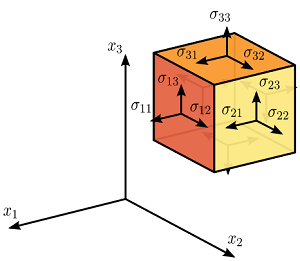
\includegraphics[width = 0.5\linewidth]{figures/Stress_vectors.png}
    \caption{Jednotlivé složky tenzoru napětí působící na krychli v~trojrozměrném prostoru.~\cite{Figure:stress_tensor}}
    \label{fig:tensor_napeti}
\end{figure}

\par \noindent
Pro úplnost uveďme, že pro těleso v~rovnováze platí:
\begin{equation}
    \tau_{ij} = \tau_{ji}.
    \label{eq:symmetry}
\end{equation}
Pro normálová napětí (tedy případ, kdy $i = j$) je toto zřejmé, pro tečná napětí však nikoliv. Pokusím se situaci objasnit: Uvažme situaci, kdy $\tau_{xy} = 0$, ale $\tau_{yx} \neq 0$. To znamená, že na stěnu kolmou k~ose $y$ působí síla, která vyvolává moment síly a~docházelo by k~rotaci tělesa. Aby tedy těleso bylo v~rovnováze, musí existovat síla, která vyruší vzniklý moment. Takovou silou je právě síla způsobující napětí $\tau_{xy}$, a~tedy musí platit výše zmíněná rovnost.\footnotemark~\cite{online:Skripta_napětí} Tenzor napětí je tedy definován šesti proměnnými: třemi vzájemně kolmými normálovými napětími $\sigma_x$, $\sigma_y$ a~$\sigma_z$ a~třemi smykovými napětími $\tau_{xy}$, $\tau_{xz}$ a~$\tau_{yz}$. \cite{wiki:Stress_mechanics}
\footnotetext{Případy, kdy rovnost ve vzorci \ref{eq:symmetry} neplatí, těleso tedy není v~rovnováze a~dochází k~otáčení, budeme probírat později trochu abstraktnějším způsobem. V~takových případech vstupuje do hry tzv.~\emph{tenzor rychlosti otáčení}.}
\par\noindent
Stejně tak mohu zkoumat mechanické napětí působící na některou, klidně až infinitezimálně malou část oné houby. Z~houby pomyslně vyříznu krychličku a~zkoumám její tenzor napětí. Tímto způsobem lze limitně získat tenzor napětí pro každý konkrétní bod.~\cite{material:Mechanika_kontinua}~\cite{wiki:Cauchy_stress_tensor}

%%%%%%%%%%%%%%%%%%%%%%%%%%%%%%%%%%%%%%%%%%%%%%%%%%%%%%%%%%%%%%%%%%%%%%
\subsection{Deformace látek dle Hookeova zákona}%%%%%%%%%%%%%%%%%%%%%%
\label{sec:Hookeův_zákon}%%%%%%%%%%%%%%%%%%%%%%%%%%%%%%%%%%%%%%%%%%%%%

Hookeův zákon říká, že pokud na pevnou látku působím normálovým napětím $\sigma$, pak toto napětí způsobí relativní prodloužení látky $\varepsilon$ dle vztahu: 
\begin{equation}
    \sigma = E\cdot\varepsilon\text{,}
\end{equation}
kde $E$ je modul pružnosti v~tahu dané konkrétní látky. Normálové napětí tedy způsobuje buď \emph{tah} nebo \emph{tlak}.
\par \noindent
Podobně když na látku působí tečné napětí $\tau$, způsobí deformaci (tzv.~skos) dle vztahu: 
\begin{equation}
    \tau = G\cdot\gamma\text{,}
    \label{eq:hook_smyk}
\end{equation}
kde $\gamma$ je úhel skosu a~$G$ je modul pružnosti ve smyku dané konkrétní látky.~\cite{wiki:Pružnost} Tečné napětí tedy způsobuje \emph{smyk}.
Vidíme, že při působení tečného napětí na pevnou látku dojde k~deformaci o~určité velikosti, a~že je pevná látka i~přes svou deformaci v~rovnovážném stavu. Určitá velikost tečného napětí odpovídá určité velikosti úhlu skosu.
\par
U kapalin je tomu jinak: modul pružnosti ve smyku $G$, jak bylo zmíněno již v~úvodu, je nulový. Při působení tečného napětí na kapalinu se nemůže rovnost \ref{eq:hook_smyk} nikdy naplnit. Ve snaze dosáhnout rovnovážného stavu se tak bude úhel skosu (a tedy i~velikost deformace) po celou dobu působení tečného napětí zvyšovat. Tento jev v~praxi pozorujeme jako \emph{tečení} kapaliny. Věda zabývající se tečením se nazývá \emph{reologie}.~\cite{wiki:Rheology} Rovnovážného stavu kapalina dojde až v~okamžiku, kdy na ní nepůsobí žádné tečné napětí, nebo když jsou všechna tečná napětí působící na kapalinu v~rovnováze.

%%%%%%%%%%%%%%%%%%%%%%%%%%%%%%%%%%%%%%%%%%%%%%%%%%%%%%%%%%%%%%%%%%%%%%
\subsection{Mechanické napětí v~kapalinách}%%%%%%%%%%%%%%%%%%%%%%%%%%%
%%%%%%%%%%%%%%%%%%%%%%%%%%%%%%%%%%%%%%%%%%%%%%%%%%%%%%%%%%%%%%%%%%%%%%

V~kapalinách (a tekutinách obecně) působí hydrostatický tlak závisející na hloubce ponoření v~kapalině (tekutině), případně může být ovlivněn vnějším působením na tekutinu. Je dán vztahem:
\begin{equation}
    p = mgh\text{.}
\end{equation}
Stejně jako pro pevné látky i~pro kapaliny lze vyjádřit tenzor napětí. Hydrostatický tlak ze své podstaty působí normálové napětí. Za normálová napětí si tedy do tenzoru deformace dosadíme hydrostatický tlak:
\begin{equation}
    \sigma_{ij} = 
    \begin{bmatrix}
        p & 0 & 0\\
        0 & p & 0\\
        0 & 0 & p
    \end{bmatrix}
    \text{.}
\end{equation}
Víme, že pokud do kapaliny ponořím krychli, součet všech hydrostatických tlaků, které na ni budou působit, se nezmění, pokud budu krychlí otáčet, a~už vůbec se nezmění v~případě, že se na krychli začnu dívat z~jiné strany. Toto je jedna z~klíčových vlastností tenzorů: existují atributy tenzoru, které se nezmění, ani pokud tenzor projde transformací souřadného systému. Pro jejich neměnnost se tyto hodnoty nazývají \emph{invarianty}. Tenzory mají invariantů několik (záleží také na tom, kolik rozměrů tenzor má). Nás však zajímá právě součet $\sigma_{xx} + \sigma_{yy} + \sigma_{zz}$, který je roven $p_x + p_y + p_z$ a~o kterém tušíme, že by měl být invariantní. Protože uvažujeme krychli nekonečně malých rozměrů, platí pro jednotlivé složky tlaků $p = p_x = p_y = p_z$, a~mohu tedy říci:
\begin{equation}
    \sigma_I = \sigma_x + \sigma_y + \sigma_z = -3p\text{,}
\end{equation}
kde $\sigma_I$ je první invariant tenzoru napětí $\sigma_{ij}$ a~$p$ je tlak. Tlak je nutný násobit $-1$, protože kladná hodnota normálového napětí by značila tah.
\par \noindent
Pro účely zkoumání proudění však není velikost hydrostatického tlaku důležitá, zajímají nás jen složky tečného napětí. Pokud znám tenzor napětí $\sigma_{ij}$ a~velikost tlaku $p$ v~bodě kapaliny, pak lze zjistit tzv.~\emph{deviátor tenzoru napětí}, který bude vyjadřovat pouze smykové napětí. Nejdříve vyjádříme tlak v~kapalině tenzorem:
\begin{equation}
    p\cdot\delta_{ij} = -\frac{1}{3}\sigma_I\cdot\delta_{ij} =
    \begin{bmatrix}
        p & 0 & 0\\
        0 & p & 0\\
        0 & 0 & p
    \end{bmatrix}
    \text{,}
\end{equation}
kde $p$ je hydrostatický tlak, $\delta_{ij}$ je tzv.~Kroneckerovo delta\footnote{Kroneckerovo delta je funkce, která se rovná $1$, pokud $i = j$, a~$0$, pokud $i \neq j$. Lze pomocí něj také popsat jednotkovou matici $n \times n$, čehož je využito právě zde.}, zde použito jako jednotková matice, a~$\sigma_I$ je první invariant tenzoru napětí $\sigma_{ij}$.~\cite{material:Hydrostatika_a_hydrodynamika}\cite{wiki:Kroneckerovo_delta}\cite{wiki:Identity_matrix}
Složky tenzoru napětí působící hydrostatický tlak na infinitezimální krychli je možné vidět na obrázku \ref{fig:tlak}.

\begin{figure}
    \centering
    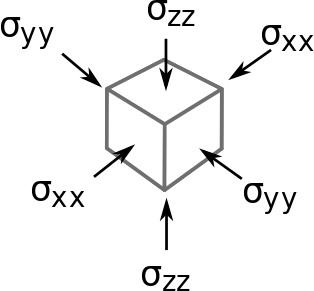
\includegraphics[width = 0.3\linewidth]{figures/Hydrostatic_Stress.png}
    \caption{Složky tenzoru napětí působící hydrostatickým tlakem na nekonečně malou krychli.~\cite{Figure:hydrostatický_tlak}}
    \label{fig:tlak}
\end{figure}

Pokud tuto tzv.~\emph{izotropní část tenzoru napětí}, značenou $\sigma_{ij}^{(i)}$ od tenzoru napětí odečteme, získáme deviátor tenzoru napětí:
\begin{equation}
    \sigma_{ij}^{(d)} = \sigma_{ij} - p\delta_{ij}\text{,}
\end{equation}
vyjadřující smykové napětí působící na kapalinu.~\cite{online:Skripta_deviátor}\cite{wiki:Deformace} Složky tohoto deviátoru pak způsobují tečení kapaliny.

%%%%%%%%%%%%%%%%%%%%%%%%%%%%%%%%%%%%%%%%%%%%%%%%%%%%%%%%%%%%%%%%%%%%%%
\subsection{Proudění a~deformace kapaliny}%%%%%%%%%%%%%%%%%%%%%%%%%%%%
%%%%%%%%%%%%%%%%%%%%%%%%%%%%%%%%%%%%%%%%%%%%%%%%%%%%%%%%%%%%%%%%%%%%%%

\subsubsection{Gradient rychlosti}%%%%%%%%%%%%%%%%%%%%%%%%%%%%%%%%%%%%

Nyní si představme houbu v~pohybu. Pokud se všechny body houby pohybují stejnou rychlostí $\vec v$, pak houba koná pouze posuvný pohyb. Pokud se však budou rychlosti jednotlivých částí houby lišit, může to znamenat dvě věci: buď houba koná kromě posuvného pohybu ještě pohyb otáčivý, nebo dochází k~deformaci houby. Pokud si v~houbě zvolíme bod, pak můžeme zjišťovat, jak se jeho rychlost liší od rychlostí sousedních bodů. Stejně tak mohu pro každý bod v~kapalině mohu zjišťovat, jak se mění tři vzájemně kolmé složky rychlosti při posunu ve směrech tří souřadných os. Této veličině říkáme \emph{gradient rychlosti} a~opět pro ní zavádíme tenzor značený $L_{ij}$. Pro tenzor gradientu rychlosti platí následující:
\begin{equation}
    L_{ij} = \nabla\vec v =
    \begin{bmatrix}
        \frac{\partial \vec{v}_x}{\partial x} & \frac{\partial \vec{v}_y}{\partial x} & \frac{\partial \vec{v}_z}{\partial x}\\
        \frac{\partial \vec{v}_x}{\partial y} & \frac{\partial \vec{v}_y}{\partial y} & \frac{\partial \vec{v}_z}{\partial y}\\
        \frac{\partial \vec{v}_x}{\partial z} & \frac{\partial \vec{v}_y}{\partial z} & \frac{\partial \vec{v}_z}{\partial z}
    \end{bmatrix}
    \text{,}
    \label{eq:tenzor_grad_rychlosti}
\end{equation}
kde $L_{ij}$ je tenzor gradientu rychlosti, $\nabla\vec v$ je jiný způsob značení gradientu vektoru rychlosti pomocí tzv.~\emph{nabla operátoru}~\cite{wiki:Nabla}, $\frac{\partial \vec{v}_i}{\partial x_j}$ jsou jednotlivé gradienty složek rychlosti (např.~$L_{23} = \frac{\partial \vec{v}_y}{\partial z}$ je gradient složky rychlosti ve směru souřadnice $y$ při posunu ve směru osy $z$ atp.).~\cite{wiki:Strain_rate_tensor}
\par
Z příkladu uvedeného výše je zřejmé, že gradient rychlosti bude souviset právě s~deformací a~rotací. Zároveň uveďme již zažitý poznatek: kde je deformace, tam je napětí.

\subsubsection{Rychlost deformace}%%%%%%%%%%%%%%%%%%%%%%%%%%%%%%%%%%%%

V~kapalinách je situace obdobná: jednotlivé částice se v~proudící kapalině pohybují rychlostí $\vec v$. Pro každý jednotlivý bod v~kapalině mohu zjistit, o~kolik se změní složka rychlosti proudění kapaliny, pokud se posunu po nějaké souřadnici. Taková změna rychlosti proudění má za následek buď rotaci, nebo jakousi deformaci kapaliny. To proto, že pokud budeme uvažovat přímočarý pohyb kapaliny, pak platí, že čím větší bude gradient rychlosti, tím větší bude rychlost deformace, a~tyto dvě hodnoty spolu tedy úzce souvisí. Pro tyto hodnoty budeme tedy opět zavádět tenzory: bude jimi \emph{tenzor rychlosti deformace}, značený $D_{ij}$, a~\emph{tenzor rychlosti otáčení}, značený $W_{ij}$, s~tím, že platí:~\cite{wiki:Strain_rate_tensor}\cite{wiki:Simple_shear}\cite{Article:Shear_pure_and_simple}
\begin{equation}
    L_{ij} = D_{ij} + W_{ij}\text{.}
    \label{eq:rovnost_tenzoru}
\end{equation}
\par
Protože kapaliny považujeme za nestlačitelné, je jedinou variantou deformace skos určený úhlem skosu $\gamma$. Konstantní gradient rychlosti však způsobuje deformaci v~čase (těleso bude postupně více a~více deformováno po celou dobu, co na něj gradient rychlosti působí). Gradient rychlosti je tedy nějakým způsobem úměrný změně úhlu skosu $\gamma$ za změnu času. Této změně úhlu skosu za změnu času se říká \emph{rychlost deformace} a~je značená $\dot\gamma$. Platí pro ni:
\begin{equation}
    \dot\gamma = \frac{\dd\gamma}{\dd t}\text{.}
    \label{eq:dot_gamma}
\end{equation}

\subsubsection{Příklad}%%%%%%%%%%%%%%%%%%%%%%%%%%%%%%%%%%%%%%%%%%%%%%%

Jak dospět k~tenzoru rychlosti deformace bude popsáno následujícím příkladem:
\par \noindent
Uvažujme řez kapalinou v~rovině určené souřadnicemi $x$ a~$y$ (existenci třetího rozměru nebudeme dále v~tomto příkladu uvažovat). Dále uvažujme čtverec určený čtyřmi body v~kapalině: $A[0,0]$, $B[\dd x,0]$, $C[\dd x,\dd y]$, $D[0,\dd y]$. Tyto body budou unášené prouděním kapaliny. Proudění kapaliny bude definované následujícím způsobem:
\begin{align}
    \begin{split}
        v_x &= 1 + y\text{,} \\
        v_y &= 1 + x\text{.}
    \end{split}
\end{align}
Rychlosti proudění v~bodech $A$, $B$, $C$, $D$ jsou pak následující:
\begin{equation}
    \vec{v}_a = (1,1)\text{,} \;
    \vec{v}_b = (1,1 + \dd x)\text{,} \;
    \vec{v}_c = (1 + \dd y,1 + \dd x)\text{,} \;
    \vec{v}_d = (1 + \dd y,1)\text{.}
\end{equation}
Nové souřadnice bodů po čase $\dd t$ jsou:
\begin{align}
    \begin{split}
        A' &= A + \vec{v}\cdot \dd t\emph{,}\\
        B'_x &= B_x + \vec{v}_x \cdot \dd t\emph{,}\\
        B'_y &= B_y + (\vec{v}_y + \frac{\partial v_y}{\partial x}\dd x) \dd t\emph{,}\\
        C'_x &= C_x + (\vec{v}_x + \frac{\partial v_x}{\partial y}\dd y) \dd t\emph{,}\\
        C'_y &= C_y + (\vec{v}_y + \frac{\partial v_y}{\partial x}\dd x) \dd t\emph{,}\\
        D'_x &= D_x + (\vec{v}_x + \frac{\partial v_x}{\partial y}\dd y) \dd t\emph{,}\\
        D'_y &= D_y + \vec{v}_y \cdot \dd t \emph{.}
    \end{split}
\end{align}
Rozdíly bodů před a~po uběhnutí času $\dd t$ jsou:
\begin{align}
    \begin{split}
        &\vec{a} = B-A = (\dd x,0)\text{,}\\
        &\vec{a}' = B'-A' = \left(\dd x + \vec{v}_x \cdot \dd t - \vec{v}_x \cdot \dd t, \left(\vec{v}_y + \frac{\partial v_y}{\partial x}\dd x\right)\dd t - \vec{v}_y \cdot \dd t\right) = \left(\dd x, \left(\frac{\partial v_y}{\partial x}\dd x\right)\dd t\right)\text{,}\\
        &\vec{d} = D-A = (0,\dd y)\text{,}\\
        &\vec{d}' = D'-A' = \left(\left(\vec{v}_x + \frac{\partial v_x}{\partial y}\dd y\right) \dd t - \vec{v}_x\cdot \dd t, \dd y + \vec{v}_y \cdot \dd t - \vec{v}_y\cdot \dd t\right) = \left(\left(\frac{\partial v_x}{\partial y}\dd y\right)\dd t,\dd y\right)\text{.}
    \end{split}
\end{align}
Taková deformace bude vypadat zhruba jako na obrázku \ref{fig:Strain}.

\begin{figure}
    \centering
    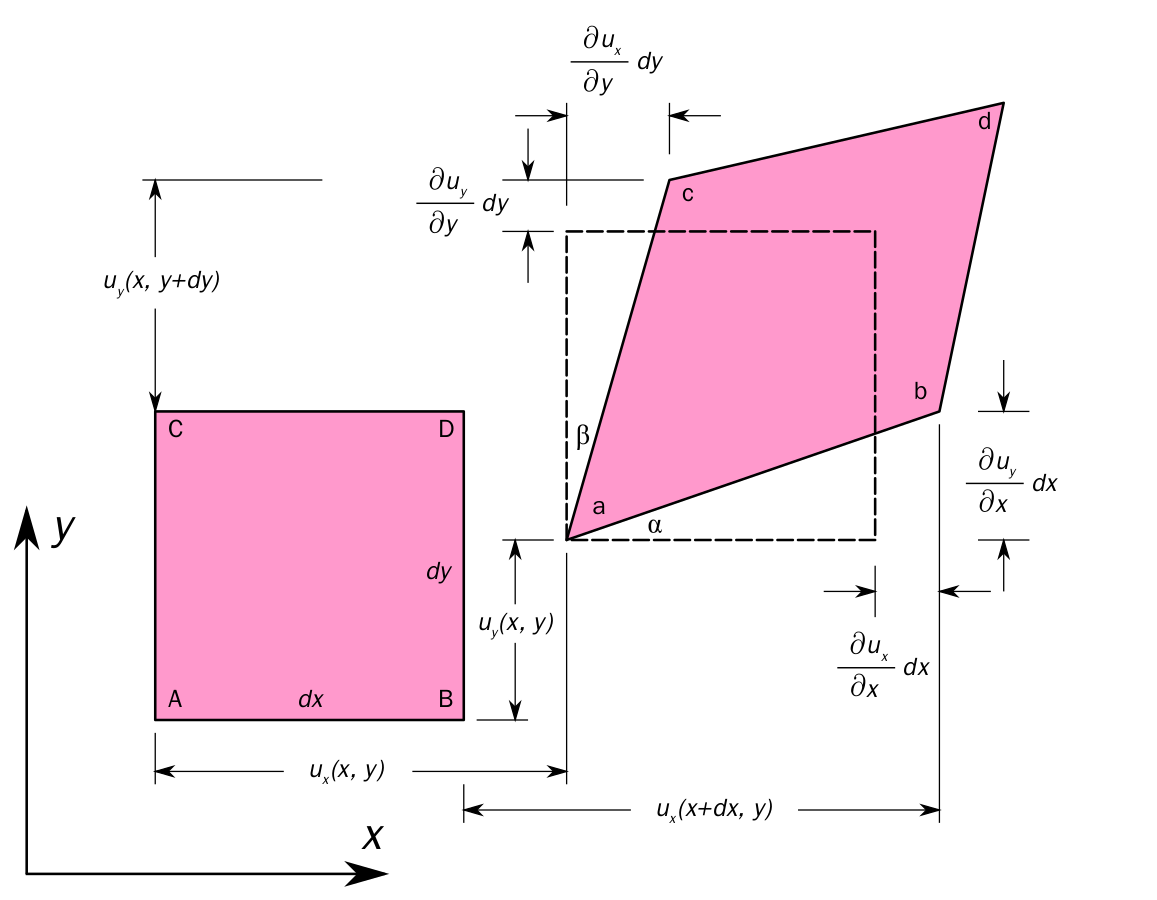
\includegraphics[width = 0.75\linewidth]{figures/2D_geometric_strain.svg.png}
    \caption{Jednoduchá deformace ve dvou rozměrech.~\cite{Figure:Strain}}
    \label{fig:Strain}
\end{figure}

Úhel skosu $\gamma_{xy}$ po čase $\dd t$, tedy rychlost deformace $\dot\gamma_{xy}$ je rovna úhlu $\dd\alpha$, který je svírán vektory $\vec{a}$ a~$\vec{a}'$, podobně je rychlost deformace $\dot\gamma_{yx}$ rovna úhlu $\dd\beta$, který je svírán vektory $\vec{d}$ a~$\vec{d}'$. Body $A$, $B$ a~$B'$ tvoří pravoúhlý trojúhelník, body $A$, $D$ a~$D'$ taktéž. Pro malé úhly můžeme předpokládat, že $\tan{\alpha} \approx \alpha$. V~našich pravoúhlých trojúhelnících platí:~\cite{YT:Kinematics_of_fluids_elements}~\cite{wiki:Strain_mechanics}~\cite{wiki:Infinitesimal_strain_theory}~\cite{wiki:Deformace}
\begin{align}
    \begin{split}
        \dd\alpha\approx\tan{\dd\alpha} &= \frac{\left|\vec{a}'-\vec{a}\right|}{\left|\vec{a}\right|} = \frac{\left(\frac{\partial v_y}{\partial x}\dd x\right)\dd t}{\dd x} = \frac{\partial v_y}{\partial x}\dd t\text{,}\\
        \dd\beta\approx\tan{\dd\beta} &= \frac{\left|\vec{d}'-\vec{d}\right|}{\left|\vec{d}\right|} = \frac{\left(\frac{\partial v_x}{\partial y}\dd y\right)\dd t}{\dd y} = \frac{\partial v_x}{\partial y}\dd t\text{.}
    \end{split}
\end{align}
Úhlovou rychlost otáčení bodu $B$ kolem bodu $A$ můžeme vyjádřit jako změnu úhlu $\dd\alpha$ za změnu času $\dd t$, obdobně to provedeme s~úhlovou rychlostí bodu $D$ kolem bodu $A$:~\cite{YT:Kinematics_of_fluids_elements}
\begin{align}
    \begin{split}
        \omega_{BA} &= \frac{\dd\alpha}{\dd t} = \frac{\partial v_y}{\partial x}\text{,}\\
        \omega_{DA} &= -\frac{\dd\beta}{\dd t} = -\frac{\partial v_x}{\partial y}\text{.}
    \end{split}
\end{align}
Úhlová rychlost $\omega_{BA}$ zároveň vyjadřuje změnu rychlosti deformace ve směru osy $y$ při posunu o~$\dd x$ vůči bodu $A$. Obdobně úhlová rychlost $-\omega_{DA}$ vyjadřuje změnu rychlosti deformace ve směru osy $x$ při posunu o~$\dd y$ vůči bodu $A$.\footnote{Vzpomeňme na definici úhlové rychlosti $\omega = \frac{v}{r}$. V~našem případě nám úhlová rychlost říká, o~kolik se změní rychlost deformace, pokud se posunu o~nějaký kus směrem od středu otáčení.}
\par
Průměrná úhlová rychlost $\omega$ sousedních bodů je pak:
\begin{equation}
    \omega = \frac{1}{2}\left(\frac{\partial v_y}{\partial x}-\frac{\partial v_x}{\partial y}\right)\text{.}
    \label{eq:omega}
\end{equation}
My rotační pohyb (tedy \emph{vorticitu proudění}) v~tomto případě neuvažujeme, tím pádem musí platit $\omega = 0$ a~tedy:
\begin{equation}
    \frac{\partial v_y}{\partial x} = \frac{\partial v_x}{\partial y}\text{.}
\end{equation}
Ve třech rozměrech analogicky platí:
\begin{align}
    \begin{split}
        \frac{\partial v_x}{\partial z} &= \frac{\partial v_z}{\partial x}\text{,}\\
        \frac{\partial v_y}{\partial z} &= \frac{\partial v_z}{\partial y}\text{.}
    \end{split}
\end{align}
Pro celkový úhel deformace $\dd\gamma$ (za čas $\dd t$) pak platí:
\begin{equation}
    \frac{\dd\gamma}{\dd t} = \frac{\partial v_y}{\partial x} + \frac{\partial v_x}{\partial y}\text{.}
    \label{eq:gradient_gamma}
\end{equation}
Jednotlivé složky rychlosti deformace pak lze vyjádřit takto:~\cite{online:Skripta_rychlost_deformace}\cite{wiki:Simple_shear}\cite{wiki:Infinitesimal_strain_theory}\cite{wiki:Deformace}
\begin{equation}
    \dot\gamma_{ij} = \frac{1}{2}\left(\frac{\partial v_j}{\partial x_i} + \frac{\partial v_i}{\partial x_j}\right) = \frac{1}{2}\frac{\dd\gamma}{\dd t}\text{.}
    \label{eq:rychlost_deformace}
\end{equation}
\par
Závěr $\dot\gamma_{ij} = \frac{1}{2}\frac{\dd\gamma}{\dd t}$ není kontradikcí vzorce \ref{eq:dot_gamma}. To proto, že $\dot\gamma$ vyjadřuje celkovou změnu úhlu skosu za čas $\dd t$, zatímco složka $\dot\gamma_{ij}$ vyjadřuje pouze složku ve směru jedné souřadnice. Tenzor rychlosti deformace $D_{ij}$ pak vyjadřuje jednotlivé složky rychlosti deformace $\dot\gamma_{ij}$.~\cite{YT:Kinematics_of_fluids_elements}\cite{online:Skripta_deformace}\cite{online:Skripta_viskozni_latky}\cite{wiki:Strain_mechanics}\cite{wiki:Infinitesimal_strain_theory}\cite{wiki:Simple_shear}
\par
V~našem dvojrozměrném příkladu pak platí následující hodnoty:
\begin{align}
    \begin{split}
        \frac{\partial v_x}{\partial x} = 0&, \;
        \frac{\partial v_y}{\partial x} = 1 \text{,}\\
        \frac{\partial v_x}{\partial y} = 1&, \;
        \frac{\partial v_y}{\partial y} = 0 \text{.}
    \end{split}
\end{align}
Připomínám\footnote{Viz vzorce \ref{eq:tenzor_grad_rychlosti}, \ref{eq:rovnost_tenzoru}, \ref{eq:omega} a~\ref{eq:rychlost_deformace}.}, že:
\begin{align}
    L_{ij} &= 
    \begin{bmatrix}
        \frac{\partial \vec{v}_x}{\partial x} & \frac{\partial \vec{v}_y}{\partial x} \\
        \frac{\partial \vec{v}_x}{\partial y} & \frac{\partial \vec{v}_y}{\partial y} \\
    \end{bmatrix}\text{,}\\
    D_{ij} &= 
    \begin{bmatrix}
        \frac{1}{2}\left(\frac{\partial v_x}{\partial x} + \frac{\partial v_x}{\partial x}\right) & \frac{1}{2}\left(\frac{\partial v_y}{\partial x} + \frac{\partial v_x}{\partial y}\right) \\
        \frac{1}{2}\left(\frac{\partial v_x}{\partial y} + \frac{\partial v_y}{\partial x}\right) & \frac{1}{2}\left(\frac{\partial v_y}{\partial y} + \frac{\partial v_y}{\partial y}\right) \\
    \end{bmatrix}\text{,}\\
    W_{ij} &=
    \begin{bmatrix}
        \frac{1}{2}\left(\frac{\partial v_x}{\partial x} - \frac{\partial v_x}{\partial x}\right) & \frac{1}{2}\left(\frac{\partial v_y}{\partial x} + \frac{\partial v_x}{\partial y}\right) \\
        \frac{1}{2}\left(\frac{\partial v_x}{\partial y} - \frac{\partial v_y}{\partial x}\right) & \frac{1}{2}\left(\frac{\partial v_y}{\partial y} + \frac{\partial v_y}{\partial y}\right) \\
    \end{bmatrix}\text{,}\\
    L_{ij} &= D_{ij} + W_{ij}\text{.} \tag{\ref{eq:rovnost_tenzoru}}
\end{align}
A tedy:
\begin{equation}
    \begin{bmatrix}
        0 & 1\\
        1 & 0
    \end{bmatrix} =
    \begin{bmatrix}
        0 & 1\\
        1 & 0
    \end{bmatrix} +
    \begin{bmatrix}
        0 & 0\\
        0 & 0
    \end{bmatrix}\text{.}
\end{equation}
Jak bylo řečeno výše, v~tomto případě je $\omega = 0$, a~tedy $L_{ij} = D_{ij}$. Gradient rychlosti v~tomto případě způsobuje pouze deformaci a~žádnou rotaci. Povšimněme si zároveň, že tenzor $D_{ij}$ je symetrický a~tenzor $W_{ij}$ je antisymetrický.~\cite{wiki:Strain_rate_tensor}

%%%%%%%%%%%%%%%%%%%%%%%%%%%%%%%%%%%%%%%%%%%%%%%%%%%%%%%%%%%%%%%%%%%%%%
\subsection{Couettovo proudění}%%%%%%%%%%%%%%%%%%%%%%%%%%%%%%%%%%%%%%%
%%%%%%%%%%%%%%%%%%%%%%%%%%%%%%%%%%%%%%%%%%%%%%%%%%%%%%%%%%%%%%%%%%%%%%

\label{sec:Couettovo_proudění}
Uvažujme řez prouděním, které je definované následujícím způsobem:
\begin{align}
    \begin{split}
        v_x = y\text{,}\\
        v_y = 0\text{.}
    \end{split}
\end{align}
Použitím znalostí z~minulé podkapitoly můžeme rovnou spočítat tenzor gradientu rychlosti:
\begin{equation}
    \begin{rcases}
        \begin{matrix}
            \dfrac{\partial v_x}{\partial x} = 0\text{,}& \;
            \dfrac{\partial v_y}{\partial x} = 0 \text{,}\\
            \dfrac{\partial v_x}{\partial y} = 1\text{,}& \;
            \dfrac{\partial v_y}{\partial y} = 0 \text{.}
        \end{matrix}
    \end{rcases}
    \;\Longrightarrow\;
    L_{ij} = 
    \begin{bmatrix}
        0 & 0 \\
        1 & 0
    \end{bmatrix}\text{,}\\
\end{equation}
Kvůli tomu, že tenzory $D_{ij}$ a~$W_{ij}$ musí splňovat vlastnosti symetrie, resp.~antisymetrie, musí platit:
\begin{equation}
    D_{ij} = 
    \begin{bmatrix}
        0 & \frac{1}{2} \\
        \frac{1}{2} & 0
    \end{bmatrix}\text{,}\\
    \;W_{ij} = 
    \begin{bmatrix}
        0 & -\frac{1}{2} \\
        \frac{1}{2} & 0
    \end{bmatrix}\text{,}\\
\end{equation}
Vidíme, že tenzor rychlosti otáčení má nenulovou hodnotu, což na první pohled nemusí dávat smysl: k~žádné rotaci v~kapalině totiž viditelně nedochází, pohyb částic v~kapalině je přímočarý. Pro vysvětlení nechť si čtenář představí výše definované proudění jako řeku. Řeka sice bude téci přímo, ale pokud do ní hodím nějaký plovoucí předmět, např. kládu, bude tato kláda prouděním otáčena kolem vlastní osy: k~nějaké rotaci tedy evidentně dochází. Jakým způsobem dochází v~kapalině ke spojení působení deformace a~rotace (popsané právě tenzory výše) snad vysvětlí obrázek \ref{fig:Deformace_couett}.

\begin{figure}
    \centering
    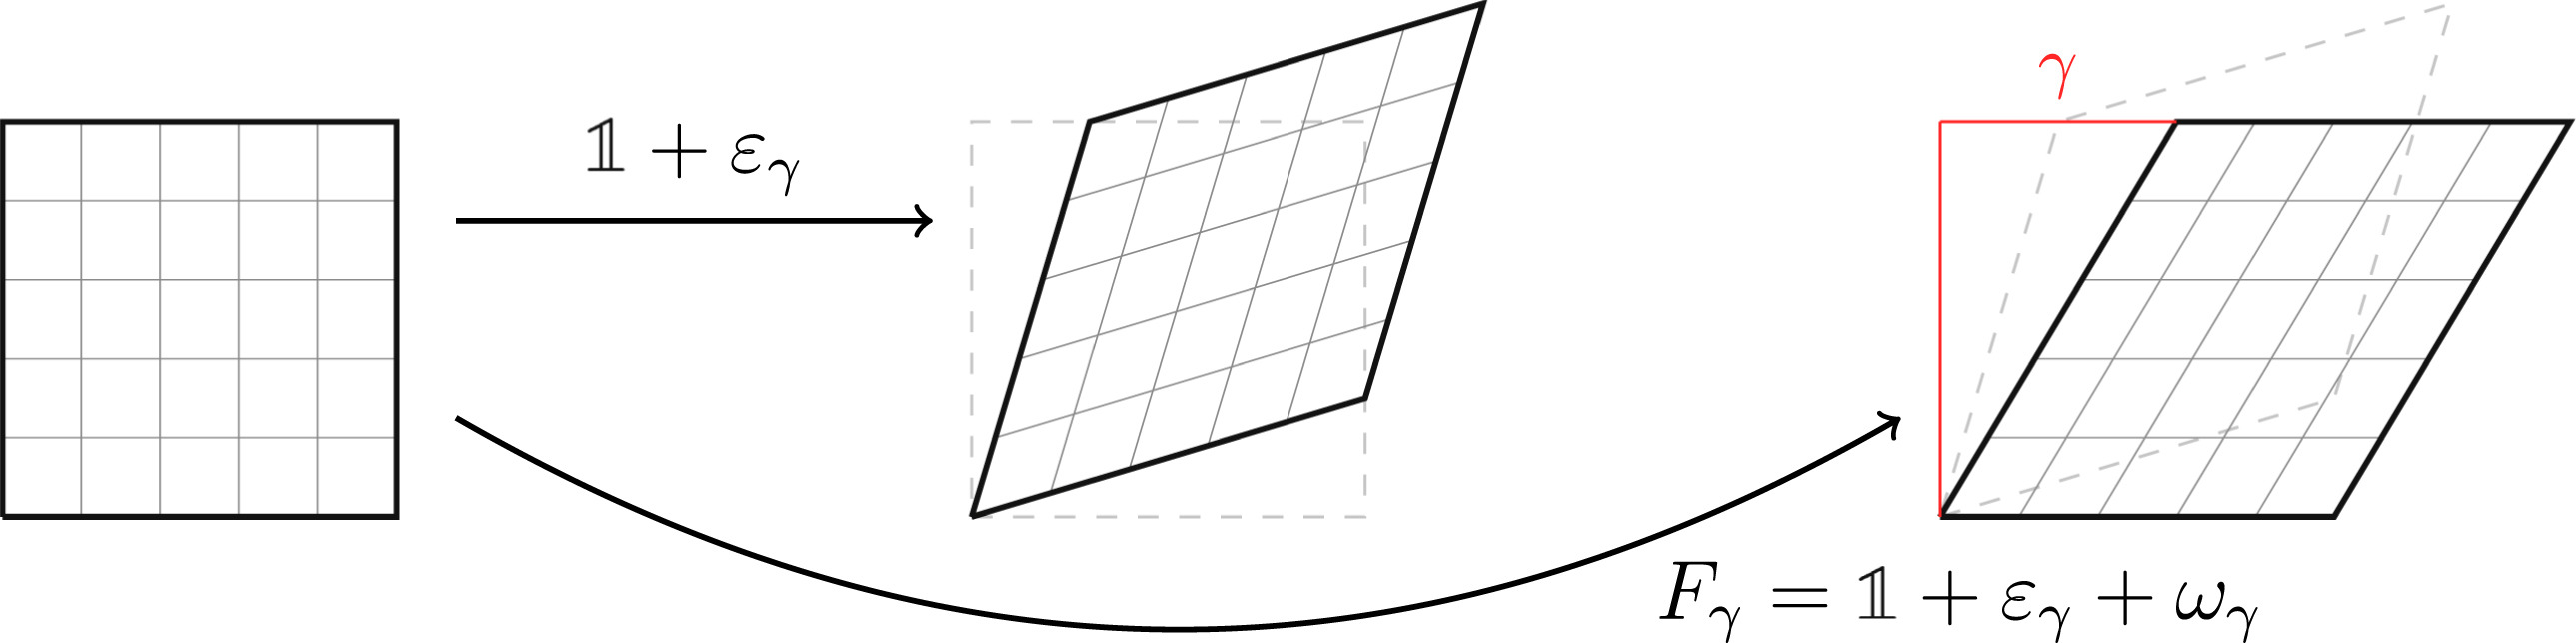
\includegraphics{figures/deformace_couett.jpg}
    \caption{Deformace v~kapalině způsobená Couettovým prouděním. Povšimněme si různého působení složky deformace a~složky rotace.~\cite{Figure:Deformace_couett}}
    \label{fig:Deformace_couett}
\end{figure}

Proudění popsané výše, tedy proudění mezi dvěma rovnoběžnými rovinami, které se vůči sobě vzájemně rovnoběžně pohybují, a~ve kterém se rychlost proudění mění ve směru kolmém na pohyb tekutiny, se nazývá \emph{Couettovo proudění}. Jedná se o~častý a~jednoduchý příklad vysvětlující pohyb kapaliny mezi dvěma deskami.~\cite{online:Skripta_rychlost_deformace} Couettovo proudění je znázorněné na obrázku \ref{fig:couett}.

\begin{figure}
    \centering
    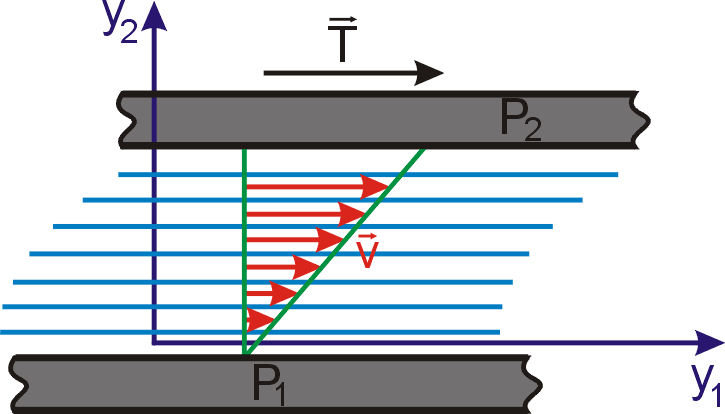
\includegraphics[width = 0.5\linewidth]{figures/couette.jpg}
    \caption{Couettovo proudění. Červené vektory $\vec{v}$ značí rychlost proudění, černý vektor $\vec{T}$ je vektor tečného napětí. Vidíme, že rychlost $\vec{v}$ stoupá ve směru souřadnice $y_2$, pro gradient rychlosti tedy platí $\frac{\partial\vec{v}_1}{\partial y_2} > 0$. Rychlost deformace $\dot\gamma$ je vyjádřena úhlem mezi dvěma zelenými úsečkami a~je ekvivalentem úhlu skosu u~pevných látek.~\cite{Figure:Skripta_couette}}
    \label{fig:couett}
\end{figure}

%%%%%%%%%%%%%%%%%%%%%%%%%%%%%%%%%%%%%%%%%%%%%%%%%%%%%%%%%%%%%%%%%%%%%%
\subsection{Viskozita u~newtonovských kapalin}%%%%%%%%%%%%%%%%%%%%%%%%
%%%%%%%%%%%%%%%%%%%%%%%%%%%%%%%%%%%%%%%%%%%%%%%%%%%%%%%%%%%%%%%%%%%%%%

V~pevných látkách je velikost napětí přímo úměrná velikosti deformace (Hookeův zákon, viz str.~\pageref{sec:Hookeův_zákon}). Sir Isaac Newton popsal, že podobně bude v~kapalinách velikost napětí přímo úměrná rychlosti deformace. V~tenzorovém zápisu platí:
\begin{equation}
    \sigma_{ij}^{(d)} = D_{ij}^{(d)}\cdot 2\eta\text{,}
\end{equation}
a obecně platí:~\cite{thesis:Viskozimetr_pro_viskozni_materialy}
\begin{equation}
    \eta\frac{\dd\gamma}{\dd t} = \eta\dot\gamma = \tau\text{,}
    \label{eq:Newtonův zákon viskozity}
\end{equation}
kde $\sigma_{ij}^{(d)}$ je deviátor napětí v~kapalině, $D_{ij}^{(d)}$ je deviátor rychlosti deformace, $\tau$ je tečné napětí a~$\frac{\dd\gamma}{\dd t}$ i~$\dot\gamma$ jsou rychlost deformace. Konstanta úměrnosti $\eta$ se nazývá \emph{dynamická viskozita} (viskozita se česky též nazývá \emph{vazkost}), má jednotku \SI{}{\pascal\second} [Pascalsekunda] a~určuje, jak rychle se bude kapalina deformovat při působení určité síly, resp.~napětí. Látky, které považujeme za husté (v laickém slova smyslu, jako například med, nikoliv ve smyslu odborném, jako třeba rtuť), mají vyšší hodnoty viskozity, než látky řídké. Viskozita tedy určuje \emph{vnitřní tření kapaliny}. V~soustavě CGS je používanou jednotkou tzv.~Poise, značený P, jehož ekvivalentem v~soustavě SI je \SI{}{\deci\pascal\second} [Decipascalsekunda]\footnotemark. Jako další užitečné veličiny jsou zaváděny \emph{tekutost} jakožto převrácená hodnota dynamické viskozity, značená $\phi$, a~\emph{kinematická viskozita}, značená $\nu$, pro kterou platí vztah:~\cite{wiki:Viskozita}
\begin{equation}
    \nu\left[\frac{\SI{}{\metre\squared}}{\SI{}{\second}}\right]= \frac{\eta}{\rho}\left[\SI{}{\pascal\second}\text{, }\SI{}{\kilo\gram\per\metre\cubed}\right]\text{,}
\end{equation}
kde $\eta$ je dynamická viskozita a~$\rho$ je hustota kapaliny.
\par
\footnotetext{Zmiňuji to proto, že mnou používaný viskozimetr měří právě v~\SI{}{\deci\pascal\second}.}
Výše popsaný \emph{Newtonův zákon viskozity} platí pro většinu jednoduchých kapalin: takové kapaliny pak nazýváme \emph{newtonovské}. Závislost mezi velikostí tečného napětí a~rychlostí deformace kapaliny je u~těchto látek lineární, proto je též nazýváme \emph{lineárně viskózní látky}. Tato vlastnost je znázorněna na obrázku \ref{fig:Newtonovská_kapalina}. Kapaliny, pro které Newtonův zákon viskozity neplatí, a~úměra mezi tečným napětím a~rychlostí deformace tedy není přímá (většinou směsi), se nazývají kapaliny \emph{nenewtonovské}.~\cite{online:Skripta_viskozni_latky}\cite{wiki:Newtonská_tekutina}

\begin{figure}
    \centering
    \includegraphics[width=\linewidth]{figures/Newtonovská_kap.png}
    \caption{Reogram newtonovské kapaliny: vzájemná závislost smykového napětí $\tau$, rychlosti deformace $\dot\gamma$ a~dynamické viskozity $\eta$ u~newtonovských kapalin.~\cite{thesis:Viskozimetr_pro_viskozni_materialy}}
    \label{fig:Newtonovská_kapalina}
\end{figure}

%%%%%%%%%%%%%%%%%%%%%%%%%%%%%%%%%%%%%%%%%%%%%%%%%%%%%%%%%%%%%%%%%%%%%%
\subsection{Nenewtonovské kapaliny}%%%%%%%%%%%%%%%%%%%%%%%%%%%%%%%%%%%
%%%%%%%%%%%%%%%%%%%%%%%%%%%%%%%%%%%%%%%%%%%%%%%%%%%%%%%%%%%%%%%%%%%%%%

Nenewtonovské látky (kapaliny) jsou takové látky, pro které Newtonův zákon viskozity neplatí. Závislost mezi tečným napětím a~rychlostí deformace tedy není lineární, ale popisuje jí nějaký jiný vztah, proto je také nazýváme \emph{látkami nelineárně viskózními}.~\cite{wiki:Newtonská_tekutina}
Vztah mezi rychlostí deformace a~tečným napětím v~kapalině $\tau = \tau(\dot\gamma)$ nebo $\dot\gamma = \dot\gamma(\tau)$ se často zakresluje do grafů (podobně jako se pro vztah $\sigma = \sigma(\varepsilon)$ pevných látek vykreslují pracovní diagramy), které se nazývají \emph{reogramy}.~\cite{material:Viskozita_a_povrchove_napeti} Křivka popisující vztah mezi rychlostí deformace a~tečným napětím se pak nazývá \emph{toková křivka}.~\cite{material:Tokove_chovani_reologicke_modely} Reogram pro čokoládu je možné vidět na obrázku \ref{fig:diagram_cokolada}.

\begin{figure}
    \centering
    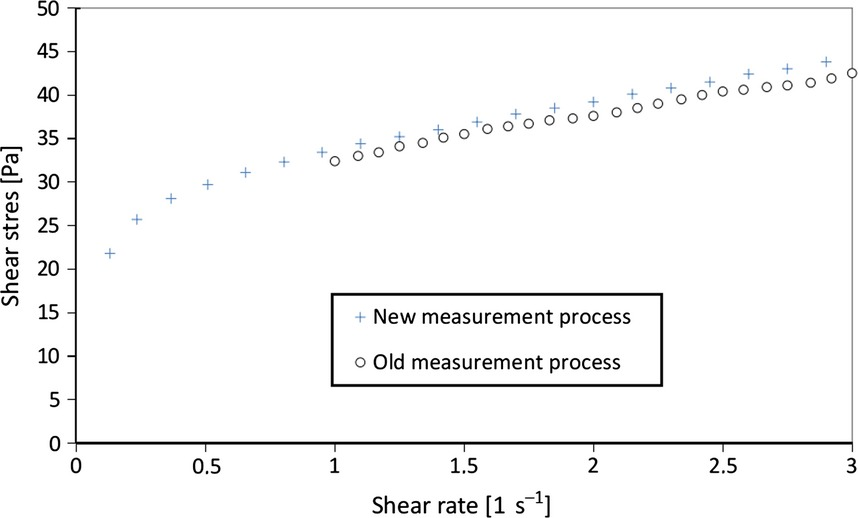
\includegraphics[width = 0.75\linewidth]{figures/diagram_viskozity_čokoláda.jpg}
    \caption{Reogram neznámé čokolády: vztah mezi rychlostí deformace (na ose $x$) a~tečným napětím (na ose $y$). Obzvlášť u~malých hodnot rychlosti deformace je zřejmé, že se nejedná o~lineární vztah. Taktéž je zde zřetelná plasticita.~\cite{Figure:chocolate_shear_stress}}
    \label{fig:diagram_cokolada}
\end{figure}

\par
Protože pro nenewtonovské kapaliny neplatí Newtonův zákon viskozity, není poměr $\frac{\tau}{\dot\gamma}$ při změnách rychlosti deformace nebo tečného napětí konstantní: viskozita tedy závisí na tečném napětí (a/nebo rychlosti deformace) a~vlastnosti kapaliny nelze popsat její jedinou hodnotou. Musíme popsat průběh viskozitu v~závislosti na ostatních veličinách. Zavádíme tzv.~\emph{zdánlivou viskozitu}, pro kterou platí:~\cite{wiki:Apparent_viscosity}
\begin{equation}
    \eta(\tau) = \frac{\tau}{\dot\gamma}\text{, nebo }\eta(\dot\gamma) = \frac{\tau}{\dot\gamma}\text{,}
    \label{eq:zdanliva_viskozita}
\end{equation}
kde $\eta(\tau)$ je zdánlivá viskozita kapaliny při smykovém napětí $\tau$ a~obdobně $\eta(\dot\gamma)$ je zdánlivá viskozita při rychlosti deformace $\dot\gamma$.
\par
Pro dokonalý popis vlastností kapaliny je nutné získat hodnoty zdánlivé viskozity při různých smykových napětích/rychlostech deformace. Měří se proto smykové napětí a~rychlost deformace, zdánlivá viskozita je pak pouhým podílem. Při vynesení tokové křivky do reogramu je pak zdánlivá viskozita směrnicí přímky vedené z~počátku souřadnic grafu do datového bodu, jak ukazuje obrázek \ref{fig:apparent_viscosity}.

\begin{figure}
    \centering
    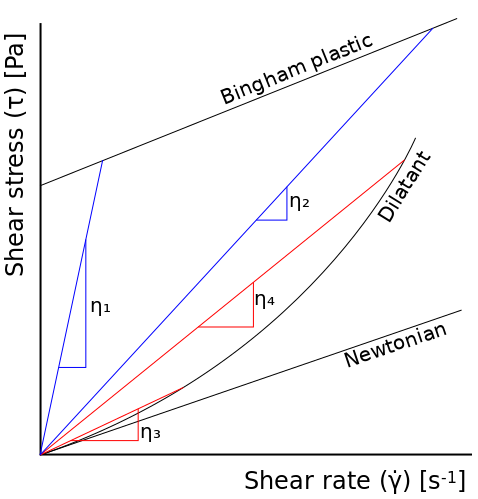
\includegraphics[width = 0.5\linewidth]{figures/Apparent_viscosity.png}
    \caption{Reogramy různých kapalin: závislosti tečného napětí (osa $y$) na rychlosti deformace (osa $x$) pro různé modely kapalin. Zatímco u~newtonovské kapaliny se jedná o~lineární vztah, zdánlivá viskozita dilatantní kapaliny s~rostoucí rychlostí deformace roste (na obrázku $\eta_4 > \eta_3$). Povšimněme si, že viskozita je v~tomto diagramu rovna směrnici přímky vedené od počátku k~datovému bodu. U~binghamské látky zdánlivá viskozita s~rostoucím tečným napětím klesá ($\eta_2 < \eta_1$), byť je toková křivka binghamské látky přímkou.~\cite{Figure:apparent_viscosity}}
    \label{fig:apparent_viscosity}
\end{figure}

\par
Nenewtonovské kapaliny pak rozlišujeme podle toho, zda při rostoucí rychlosti deformace zdánlivá viskozita roste či klesá. Látky, u~kterých zdánlivá viskozita s~rostoucí rychlostí deformace roste, nazýváme \emph{dilatantní}, naopak látky, u~kterých zdánlivá viskozita s~rostoucí rychlostí deformace klesá, nazýváme \emph{pseudoplastické}. Tokové křivky popisující chování nejen dilatantních a~pseudoplastických látek jsou znázorněny na obrázku \ref{fig:rheology_diagram}.

\begin{figure}
    \centering
    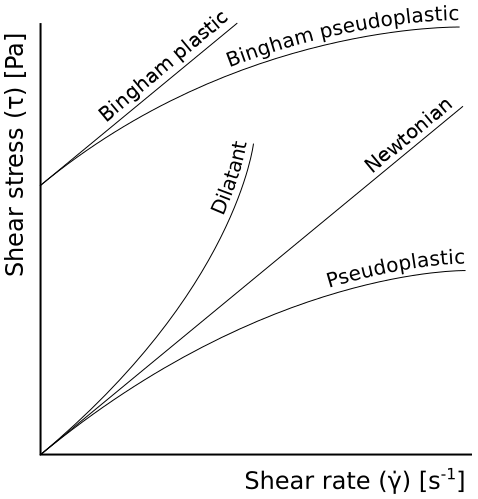
\includegraphics[width = 0.5\linewidth]{figures/Rheology_of_time_independent_fluids.png}
    \caption{Reogramy různých kapalin: závislosti tečného napětí (osa $y$) na rychlosti deformace (osa $x$) pro různé modely kapalin. Zdánlivá viskozita dilatantní kapaliny s~rostoucí rychlostí deformace roste, u~pseudoplastické kapaliny klesá.~\cite{Figure:rheology_diagram}}
    \label{fig:rheology_diagram}
\end{figure}

\subsubsection{Dilatantní látky}%%%%%%%%%%%%%%%%%%%%%%%%%%%%%%%%%%%%%%

U dilatantních látek se zdánlivá viskozita s~rostoucí rychlostí deformace zvyšuje. Dilatance není častým příkladem nenewtonovského chování kapalin a~vyskytuje se hlavně u~suspenzí a~koloid. Ve stabilizované suspenzi nebo koloidě jsou rozptýlené částice rovnoměrně rozmístěné v~kapalině a~odpudivé síly, které mezi jednotlivými částicemi působí, jsou v~rovnováze. Při deformaci jsou rozptýlené částice nuceny se vzájemně přiblížit a~dochází k~jejich oddělení ze směsi (tzv.~\emph{flokulaci}).~\cite{wiki:Flocculation}\cite{prez:teorie_koagulace} Dochází pak k~interakci mezi jednotlivými pevnými částicemi a~směs se (alespoň velmi částečně) začne chovat jako pevná látka. Tím dojde ke zvýšení odporové síly a~tedy i~viskozity.~\cite{wiki:Dilatant}
\par
Nejčastěji demonstrovaným příkladem je (i ve školním prostředí) směs vody a~kukuřičného škrobu. Chování dilatantní látky je znázorněno na obrázku \ref{fig:dilatantní_kap}.

\begin{figure}
    \centering
    \includegraphics[width=\linewidth]{figures/Dilatantní_kap.png}
    \caption{Reogram dilatantní kapaliny: vzájemná závislost smykového napětí $\tau$, rychlosti deformace $\dot\gamma$ a~dynamické viskozity $\eta$.~\cite{thesis:Viskozimetr_pro_viskozni_materialy}}
    \label{fig:dilatantní_kap}
\end{figure}

\subsubsection{Pseudoplastické látky}%%%%%%%%%%%%%%%%%%%%%%%%%%%%%%%%%

U pseudoplastických látek zdánlivá viskozita s~rostoucí rychlostí deformace klesá. Přesné příčiny pseudoplasticity nejsou ještě dokonale prozkoumané, obecně se však má za to, že je způsobená přeuspořádáním částic v~kapalině při deformaci. U~suspenzí, které jsou tvořeny polymery, dochází při deformaci k~jejich vzájemnému rozmotání a~natočení se rovnoběžně se směrem deformace. Tím je zvýšena vzdálenost mezi jednotlivými částicemi a~síla jejich vzájemných interakcí tedy slábne: viskozita klesá.~\cite{wiki:Shear_thinning}
\label{sec:pseudoplasticita}
\par
Nejčastěji se pseudoplasticita vyskytuje u~suspenzí tvořených dlouhými řetězci nebo obecně u~takových, které mají komplexní strukturu. Praktickými příklady jsou některé jedlé kapalné směsi (kečup\footnote{Čtenář má jistě s~kečupem praktickou zkušenost: teče tím snáze, čím větším tečným napětím na něj působíme.}, šlehačka), krev, nebo různé laky/barvy.~\cite{wiki:Shear_thinning} Chování pseudoplastické látky je znázorněno na obrázku \ref{fig:pseudoplast_kap}.

\begin{figure}
    \centering
    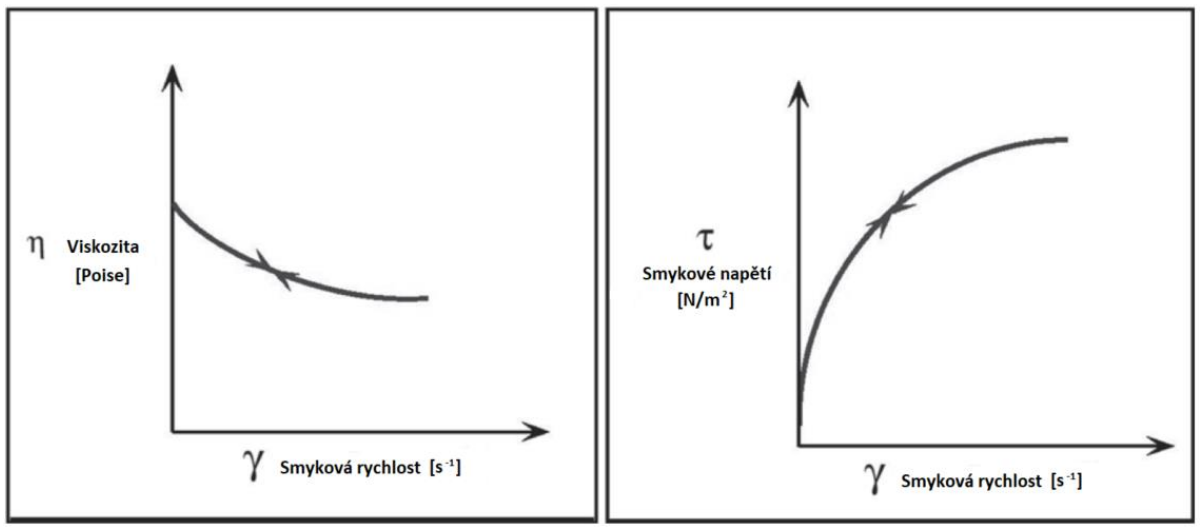
\includegraphics[width=\linewidth]{figures/Pseudoplast_kap.png}
    \caption{Reogram pseudoplastické kapaliny: vzájemná závislost smykového napětí $\tau$, rychlosti deformace $\dot\gamma$ a~dynamické viskozity $\eta$.~\cite{thesis:Viskozimetr_pro_viskozni_materialy}}
    \label{fig:pseudoplast_kap}
\end{figure}

%%%%%%%%%%%%%%%%%%%%%%%%%%%%%%%%%%%%%%%%%%%%%%%%%%%%%%%%%%%%%%%%%%%%%%
\subsection{Časová závislost viskozity}%%%%%%%%%%%%%%%%%%%%%%%%%%%%%%%
%%%%%%%%%%%%%%%%%%%%%%%%%%%%%%%%%%%%%%%%%%%%%%%%%%%%%%%%%%%%%%%%%%%%%%

Viskozita kapaliny (a tedy rychlost její deformace) však kromě velikosti tečného napětí může záviset i~na tom, jak dlouho tímto smykovým napětím na kapalinu působíme. Pokud například budeme na pseudoplastickou kapalinu působit určitým tečným napětím jen po zlomek sekundy, nestihne dojít ke změně orientace částic v~kapalině a~viskozita zůstane téměř neměnná. Se zvyšující se délkou trvání působení tečného napětí v~kapalině bude viskozita postupně klesat. Rozlišujeme tedy opět dva druhy látek:
\begin{itemize}[noitemsep, topsep = 0pt]
    \item Látky, u~kterých při působení stálého tečného napětí rychlost deformace se stoupající dobou působení klesá (viskozita tedy roste). Takové látky nazýváme \emph{reopexní}.
    \item Látky, u~kterých při působení stálého tečného napětí rychlost deformace se stoupající dobou působení roste (viskozita tedy klesá). Takové látky nazýváme \emph{tixotropní}.
\end{itemize}

\subsubsection{Reopexní látky}%%%%%%%%%%%%%%%%%%%%%%%%%%%%%%%%%%%%%%%%

U reopexních látek (někdy též \emph{antitixotropních} látek) viskozita s~dobou působení napětí roste (například při třepání postupně tuhnou). Příčiny reopexního chování kapalin nejsou ještě plně prozkoumány, nejspíše je však způsobeno postupnou koagulací rozptýlených látek v~kapalině, která je deformací vyvolána, nebo dokonce úplnou krystalizací některých z~kapalných složek směsi.~\cite{Article:Thixotropy}\cite{wiki:Time-dependent_viscosity}
\par
Reopexe je poměrně vzácným úkazem. Reopexními vlastnostmi se však vyznačují například tonery do tiskáren, kloubní maz nebo některá průmyslová maziva.~\cite{wiki:Rheopecty}

\subsubsection{Tixotropní látky}%%%%%%%%%%%%%%%%%%%%%%%%%%%%%%%%%%%%%%

U tixotropních látek dochází při působení tečného napětí v~kapalině k~postupnému snížení viskozity. Příčiny tixotropního chování jsou nejspíše totožné s~příčinami pseudoplasticity (viz str. \pageref{sec:pseudoplasticita}). Přeuspořádání částic v~kapalině však nějakou dobu trvá, naopak při uvolnění napětí se částice dlouhou dobu dostávají do méně uspořádaného stavu. Z~tohoto důvodu zde dochází k~tzv.~\emph{hysterezi}: látka si nějakou dobu \glqq pamatuje\grqq, jakou deformaci podstoupila. Při uvolnění napětí se tedy zdánlivá viskozita nevrací po téže křivce. Toto je znázorněné na obrázku \ref{fig:tixotropni_kap}.~\cite{thesis:Viskozimetr_pro_viskozni_materialy}
\par
Příkladů tixotropních látek je v~porovnání s~ostatními druhy nenewtonovských kapalin mnoho (už jen kvůli principu jejich fungování). Z~přírody např. tekutý písek, některé jíly a~bahna, med nebo tělní tekutiny (lidské semeno).~\cite{wiki:Thixotropy} Z~dalších uveďme například jogurt, cement, nebo pájecí pasty.~\cite{Article:Thixotropy}\cite{Article:cement}\cite{thesis:Viskozimetr_pro_viskozni_materialy}\cite{wiki:Time-dependent_viscosity}

\begin{figure}
    \centering
    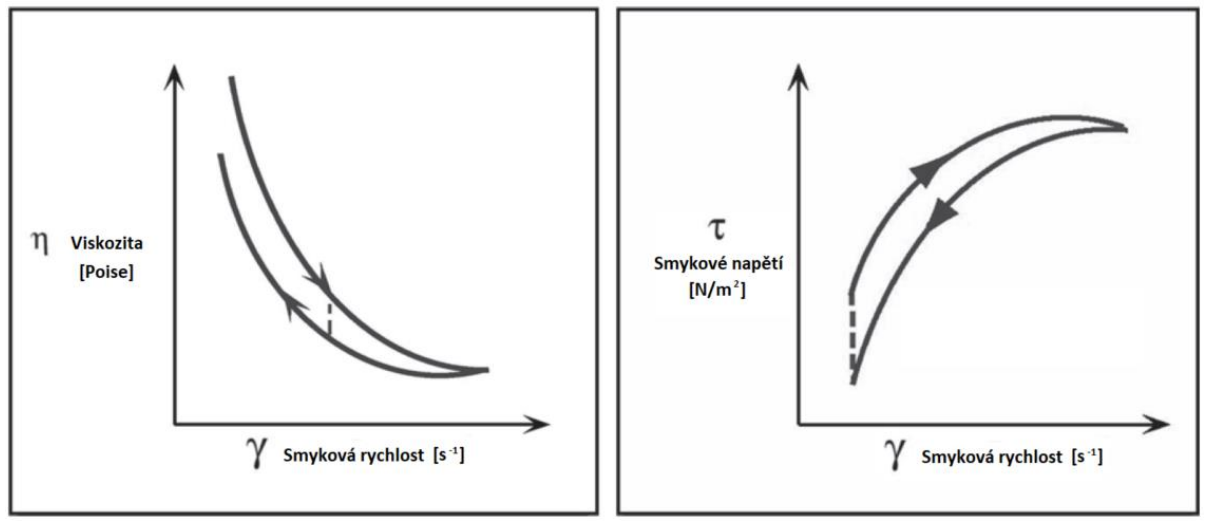
\includegraphics[width=\linewidth]{figures/tixotropni_hystereze.png}
    \caption{Reogram tixotropní látky: vzájemná závislost smykového napětí $\tau$, rychlosti deformace $\dot\gamma$ a~dynamické viskozity $\eta$. Zde je evidentní hystereze kapaliny, křivky zdánlivé viskozity jsou různé při zvyšování a~snižování smykového napětí.~\cite{thesis:Viskozimetr_pro_viskozni_materialy}}
    \label{fig:tixotropni_kap}
\end{figure}

%%%%%%%%%%%%%%%%%%%%%%%%%%%%%%%%%%%%%%%%%%%%%%%%%%%%%%%%%%%%%%%%%%%%%%
\subsection{Modelování chování nenewtonovských kapalin}%%%%%%%%%%%%%%%
%%%%%%%%%%%%%%%%%%%%%%%%%%%%%%%%%%%%%%%%%%%%%%%%%%%%%%%%%%%%%%%%%%%%%%

Jak bylo popsáno výše, vztah mezi (zdánlivou) viskozitou a~tečným napětím není u~nenewtonovských kapalin lineární. Každá nenewtonovská kapalina má specifický profil závislosti viskozity na tečném napětí. Abychom mohli popsat chování nenewtonovských kapalin, musíme nejdříve popsat průběh viskozity v~závislosti na tečném napětí. Vyjádřit tento vztah se snaží různé modely. Nejjednodušší z~nich se nazývá \emph{Ostwaldova-deWaaleova rovnice} a~má tvar:~\cite{online:Skripta_viskozni_latky}\cite{wiki:Power-law_fluid}
\begin{equation}
    \tau = \eta^{*}\dot\gamma^n\text{.}
    \label{eq:ostwald_dewaale}
\end{equation}
Pro zdánlivou viskozitu při dané rychlosti deformace $\eta(\dot\gamma)$ pak platí:
\begin{equation}
    \eta(\dot\gamma) = \frac{\tau}{\dot\gamma} = \eta^*\dot\gamma^{n-1}\text{.}
\end{equation}
Konstanta $\eta^*$ vyjadřuje zdánlivou viskozitu kapaliny při smykovém napětí, které se limitně blíží $0$, a~v~angličtině se pro ni používá termín \glqq index konsistence\grqq\space(často je též značená písmenem $k$). Proměnná $n$ pak vyjadřuje chování kapaliny. Pro pseudoplastické kapaliny platí $n < 1$, pro dilatantní kapaliny platí $n > 1$, a~pro newtonovské kapaliny evidentně platí $n = 1$ (Ostwaldova-deWaaleova rovnice je pak redukována na Newtonův zákon viskozity).
\par
Pro kapaliny, jejichž chování je složitější, vznikají jiné modely, které se snaží lépe aproximovat chování dané konkrétní kapaliny. Viskozitní modely relevantní pro chování čokolády budou diskutovány ve vlastní kapitole na str.~\pageref{sec:Reologické_vlastnosti_čokolády} a~následujících.

%%%%%%%%%%%%%%%%%%%%%%%%%%%%%%%%%%%%%%%%%%%%%%%%%%%%%%%%%%%%%%%%%%%%%%
\newpage%%%%%%%%%%%%%%%%%%%%%%%%%%%%%%%%%%%%%%%%%%%%%%%%%%%%%%%%%%%%%%
\section{Viskozimetry}%%%%%%%%%%%%%%%%%%%%%%%%%%%%%%%%%%%%%%%%%%%%%%%%
%%%%%%%%%%%%%%%%%%%%%%%%%%%%%%%%%%%%%%%%%%%%%%%%%%%%%%%%%%%%%%%%%%%%%%
%%%%%%%%%%%%%%%%%%%%%%%%%%%%%%%%%%%%%%%%%%%%%%%%%%%%%%%%%%%%%%%%%%%%%%

K~měření viskozity kapalin (nebo kapalných směsí) se využívají přístroje zvané \emph{viskozimetry}. Viskozimetry většinou měří zdánlivou viskozitu, protože je měření prováděno při neznámém tečném napětí/rychlosti deformace. To z~principu nevadí u~newtonovských kapalin. Přístroje, které kromě viskozity měří i~smykové napětí nebo rychlost deformace, při kterých byla viskozita měřena, a~jsou tedy vhodné k~měření tokových křivek nenewtonovských kapalin, se správně nazývají \emph{reometry}.~\cite{wiki:Viscometer}
\par
Stejně jako u~měřicích přístrojů pro měření většiny ostatních veličin, i~u viskozimetrů existuje několik různých konstrukcí, kdy každá pro měření dané veličiny používá jiného principu. Viskozimetry využívají k~posouzení viskozity vždy jednu konkrétní vlastnost kapaliny, konkrétně:
\begin{itemize}[noitemsep, topsep = 0pt]
    \item Rychlost tečení kapaliny (trubicí/kapilárou), která závisí na viskozitě (jakožto vnitřním tření). Na tomto principu fungují kapilární a~nálevkové viskozimetry.
    \item Odpor, který kapalina klade tělesu, které se v~ní pohybuje. Velikost tohoto odporu závisí na viskozitě. Na tomto principu fungují tělískové a~rotační viskozimetry.
\end{itemize}
Tyto druhy viskozimetrů si dovolím krátce popsat.

%%%%%%%%%%%%%%%%%%%%%%%%%%%%%%%%%%%%%%%%%%%%%%%%%%%%%%%%%%%%%%%%%%%%%%
\subsection{Kapilární viskozimetry}%%%%%%%%%%%%%%%%%%%%%%%%%%%%%%%%%%%
%%%%%%%%%%%%%%%%%%%%%%%%%%%%%%%%%%%%%%%%%%%%%%%%%%%%%%%%%%%%%%%%%%%%%%

Kapilární viskozimetry pracují na principu měření času, za který určitý objem kapaliny proteče skrz tenkou trubici kruhového průřezu (tj.~kapiláru). Proto si nyní teoreticky popíšeme proudění kapaliny válcovou trubicí.

\subsubsection{Tečení kapaliny trubicí, odvození Hagenova-Poiseulleova zákona}
\label{sec:tečení_trubicí}%%%%%%%%%%%%%%%%%%%%%%%%%%%%%%%%%%%%%%%%%%%%

Při proudění kapaliny skrz trubici platí, že rychlost proudění je nejvyšší ve středu trubice (uvažujeme laminární proudění). Kapalina je v~mezní vrstvě těsně u~stěny vůči stěně v~klidu, čím více se přibližujeme ke středu proudění, tím rychlejší je proudění kapaliny. Existuje zde tedy gradient rychlosti, jelikož se rychlost mění vzhledem ke vzdálenosti od osy trubice. V~zásadě se jedná o~případ podobný Couettovu proudění (viz str.~\pageref{sec:Couettovo_proudění}), jen se nepohybujeme v~rovině, nýbrž ve válci. Použitím vzorců č.~\ref{eq:dot_gamma} a~\ref{eq:gradient_gamma} můžeme rychlost deformace kapaliny v~trubici vyjádřit vztahem:~\cite{book:Calibration_of_viscometers}
\begin{equation}
    \dot\gamma = -\frac{\dd v}{\dd r}\text{,}
    \label{eq:gamma_gradient}
\end{equation}
kde $v$ je rychlost proudění a~$r$ je vzdálenost od osy trubice. Dle Newtonova zákona viskozity (vzorec č.~\ref{eq:Newtonův zákon viskozity}, str.~\pageref{eq:Newtonův zákon viskozity}) pak platí, že tečné napětí v~kapalině bude rovno:~\cite{book:Calibration_of_viscometers}
\begin{equation}
    \tau = -\eta\frac{\dd v}{\dd r}\text{.}
\end{equation}

\begin{figure}
    \centering
    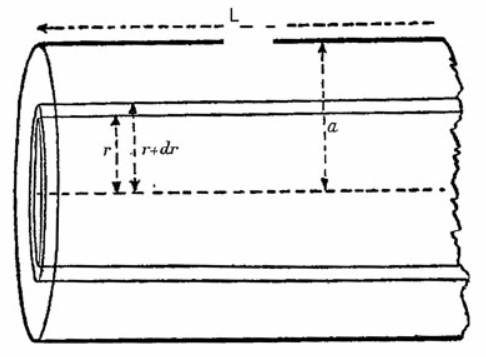
\includegraphics[width=0.5\linewidth]{figures/valce_kapaliny.png}
    \caption{Znázornění kapalinových válců v~trubici.~\cite{book:Calibration_of_viscometers}}
    \label{fig:valce}
\end{figure}

Můžeme si představit, že kapalina je tvořena nekonečným množstvím soustředných dutých válců (jejichž plášť je nekonečně tenký). Znázornění těchto válců je na obrázku~\ref{fig:valce}. Tyto kapalinové válce se v~sobě vůči sobě navzájem pohybují, a~na každý z~nich působí tečné napětí. Toto tečné napětí působí na plochu kapaliny, která je rovna povrchu pláště našeho válce $S'$. Ten je roven:~\cite{book:Calibration_of_viscometers}
\begin{equation}
    S' = 2\pi rl\text{,}
\end{equation}
kde $r$ je poloměr válce (tj.~vzdálenost stěny válce od osy trubice) a~$l$ je délka trubice. Použitím vzorce č.~\ref{eq:napeti_tau} získáváme, že viskózní odporová síla působící na daný válec je rovna:~\cite{book:Calibration_of_viscometers}
\begin{equation}
    F_\eta = \tau\cdot S' = -2\pi rl\eta\frac{\dd v}{\dd r}\text{.}
\end{equation}
Na každý z~těchto válců působí tlaková síla, která kapalinu žene trubicí. Pro tu platí:~\cite{book:Calibration_of_viscometers}
\begin{equation}
    F_p = \Delta p\cdot S = \Delta p\pi r^2\text{,}
\end{equation}
kde $\Delta p$ je tlak působící na kapalinu, $S$ je průřez trubice a~$r$ je poloměr válce. Pokud kapalina koná rovnoměrný pohyb, jsou síly $F_\eta$ a~$F_p$ v~rovnováze. Platí tedy:~\cite{book:Calibration_of_viscometers}
\begin{align}
    \begin{split}
        \Delta p\pi r^2 &= -2\pi rl\eta\frac{\dd v}{\dd r}\text{,}\\
        \Delta pr &= -2l\eta\frac{\dd v}{\dd r}\text{,}\\
        \frac{\dd v}{\dd r} &= -\frac{\Delta pr}{2l\eta}\text{.}
    \end{split}
\end{align}
Rychlost proudění $v$ ve vzdálenosti $(R-r)$ od stěny trubice (kde $R$ je poloměr trubice) je pak určena takto:~\cite{book:Calibration_of_viscometers}
\begin{equation}
    v = \int \frac{\dd v}{\dd r} \dd (R-r) = \int \frac{\Delta pr}{2l\eta} \dd (R-r) = \frac{\Delta p}{2l\eta}\int r\dd (R-r)\text{.}
\end{equation}
Položíme $x = (R-r)$, pak $r = -x+R$:
\begin{equation}
    v = \frac{\Delta p}{2l\eta}\int(-x+R) \dd x = \frac{\Delta p}{2l\eta}\cdot(\frac{-x^2}{2}+Rx)\text{.}
\end{equation}
Dosazením $(R-r)$ zpět za $x$ dostáváme:
\begin{align}
    \begin{split}
        v &= \frac{\Delta p}{2l\eta}\cdot\left(\frac{-R^2+2Rr-r^2}{2}+R^2-Rr\right)\text{, a~tedy:}\\
        v &= \frac{\Delta p}{4l\eta}(R^2-r^2)\text{.}
        \label{eq:rychlost_hagen_poiseull}
    \end{split}
\end{align}
Každým z~námi uvažovaných válců proudí určité množství kapaliny. Průřez takovým dutým válcem s~tloušťkou stěny $\dd r$ kolmo na jeho osu je vlastně mezikruží, které bude mít obsah:
\begin{equation}
    S = 2\pi r\dd r\text{.}
    \label{eq:obsah_hagen_poiseull}
\end{equation}
Pro průtok kapaliny platí vztah $Q = Sv$. Dosazením ze vzorce \ref{eq:obsah_hagen_poiseull} dostáváme, že průtok $\dd Q$ jedním infinitezimálním válcem je:~\cite{book:Calibration_of_viscometers}
\begin{equation}
    \dd Q = 2\pi r\dd rv\text{.}
\end{equation}
Průtok celou trubicí je pak součtem průtoků všemi infinitezimálními válci (kterých je nekonečně mnoho). Dosadíme tedy rychlost ze vztahu \ref{eq:rychlost_hagen_poiseull} a~opět zintegrujeme vzhledem k~$r$:~\cite{book:Calibration_of_viscometers}
\begin{align}
    \begin{split}
        Q &= \int_0^R\left(2\pi r\cdot \frac{\Delta p}{4l\eta}(R^2-r^2)\right)\dd r = \frac{2\pi\Delta p}{4l\eta}\int_0^R r(R^2-r^2)\dd r\\
        Q &= \frac{\pi\Delta pR^4}{8l\eta}
    \end{split}
\end{align}
Tento vztah se nazývá \emph{Hagenův-Poiseulleův zákon}. Jeho úpravami lze získat:~\cite{wiki:Hagen-Poiseulle_equation}\cite{thesis:Viskozimetr_pro_viskozni_materialy}
\begin{equation}
    Q = \frac{\Delta pS^2}{8\pi l\eta}\text{, a~tedy: } \eta = \frac{\Delta ptS^2}{8\pi lV}\text{,}
    \label{eq:Hagen_Poiseull}
\end{equation}
kde $\Delta p$ tlak, který kapalinu žene, $\eta$ je dynamická viskozita kapaliny, $l$ je délka trubice (kapiláry), $Q$ je průtok, pro který platí $Q=\frac{V}{t}$, kde $V$ je objem kapaliny, který protekl trubicí za čas $t$, $r$ je poloměr trubice (kapiláry) a~$S$ je průřez trubice (kapiláry). V~kapilárních viskozimetrech je jedinou hnací silou tíhová síla kapaliny a~jediný tlak, který zde působí, je hydrostatický tlak kapaliny. Platí tedy:
\begin{equation}
    \Delta p = h\rho g \text{, a~tedy: }\eta = \frac{h\rho gtS^2}{8\pi lV}\text{.}
\end{equation}
Jelikož $h$, $g$, $S$, $8$, $\pi$, $l$ a~$V$ jsou konstanty, zahrnují se většinou do jedné \emph{přístrojové konstanty} $k$, pro kterou platí:
\begin{equation}
    k = \frac{hgS^2}{8\pi lV}\left[\frac{\SI{}{\milli\metre\squared}}{\SI{}{\second\squared}}\right]\text{.}
\end{equation}
Pro kapilární viskozimetry tedy platí vztah:
\begin{equation}
    \nu\left[\frac{\SI{}{\milli\metre\squared}}{\SI{}{\second}}\right] = \frac{\eta}{\rho}\left[\SI{}{\milli\pascal\second}\text{, } \frac{\SI{}{\gram}}{\SI{}{\centi\meter\cubed}}\right]= kt\left[\frac{\SI{}{\milli\metre\squared}}{\SI{}{\second\squared}}\text{, }\SI{}{\second}\right]\text{,}\label{eq:kapilarni_viskozimetr}
\end{equation}
kde $\nu$ je kinematická viskozita kapaliny, $\eta$ je dynamická viskozita kapaliny, $k$ je konstanta viskozimetru a~$t$ je čas, za který kapalina viskozimetrem protekla.
\par
Ve skutečných viskozimetrech je pro naprostou přesnost ještě nutné uvažovat různé korekční faktory (aerostatický vztlak působící na kapalinu, tepelná roztažnost viskozimetru, změna teploty měřené kapaliny během měření a~další)~\cite{book:Calibration_of_viscometers}, my je však uvažovat nebudeme.

\subsubsection{Konstrukce a~použití}%%%%%%%%%%%%%%%%%%%%%%%%%%%%%%%%%%

Kapilární viskozimetry se vyrábí ze skla a~mají tvar U-trubice. Část U-trubice (kapilára) je zúžena na přesně kalibrovaný průměr. Jedno rameno viskozimetru se naplní kapalinou až po plnicí rysku. Hladiny v~ramenech tedy nejsou ve stejné výšce a~kapalina není v~rovnováze (je hnána vlastním hydrostatickým tlakem). Po uvolnění zátky je kapalině umožněno tečení, kapalina protéká skrz kapiláru. Měřen je čas, za který kapilárou proteče určitý objem kapaliny. Dle Hagenova-Poiseullova zákona (\ref{eq:Hagen_Poiseull}), respektive dle převodního vztahu kapilárních viskozimetrů (\ref{eq:kapilarni_viskozimetr}) lze z~tohoto času spočítat viskozitu. Přístrojová konstanta je zjišťována výrobcem a~nejčastěji uvedena na těle přístroje. Viskozimetr by měl být po celou dobu měření ponořen ve vodní lázni.
\par
Podle toho, zda kapalina během tečení teče do nebo z~měřicí baňky rozlišujeme viskozimetry \glqq pro neprůhledné kapaliny\grqq\space(někdy též nazývané \emph{zpětné viskozimetry}) a~\glqq pro průhledné kapaliny\grqq.~\cite{book:Calibration_of_viscometers} To proto, že pokud by se neprůhledná kapalina (jako třeba čokoláda) měřila vytékáním z~měřicí baňky, smočila by nejdříve její stěny a~nebylo by vidět, že kapalina již vytekla. Neprůhlednou kapalinu lze tedy měřit pouze tak, že do baňky vtéká.
\par
Konstrukcí kapilárních viskozimetrů existuje celá řada. Nejrozšířenějším typem kapilárního viskozimetru pro průhledné kapaliny je \emph{viskozimetr dle Ubbelohdeho}. Dalším často používaným typem je, pro jednoduchost svého provedení, \emph{viskozimetr dle Ostwalda}, ať už v~provedení pro průhledné nebo neprůhledné kapaliny. Nákresy těchto typů viskozimetrů jsou na obrázku~\ref{fig:viskozimetry}. Použití jednotlivých typů viskozimetrů bude popsáno níže.

\begin{figure}
    \begin{subfigure}[b]{.3\textwidth}
        \captionsetup{justification=centering}
        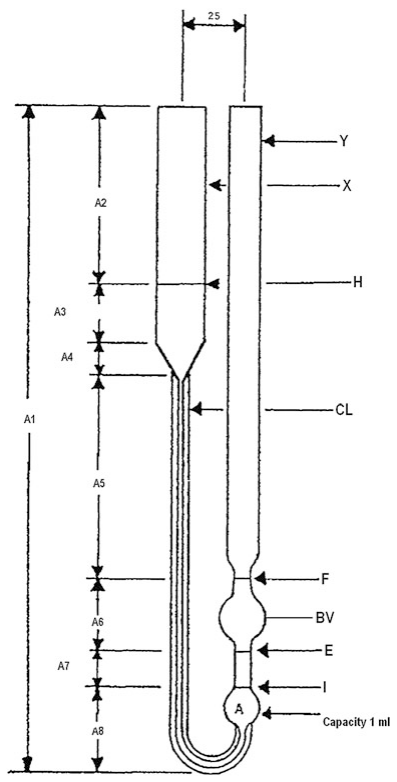
\includegraphics[height=0.4\paperheight]{figures/ostwald.png}
        \caption{X - zásobní nádoba;\\H,I - plnicí rysky;\\CL - kapilára;\\E,F - měřicí rysky;\\BV - měřicí baňka.}
        \label{sfig:Ostwald_zpetny}
    \end{subfigure}
    \hfill
    \begin{subfigure}[b]{.3\textwidth}
        \captionsetup{justification=centering}
        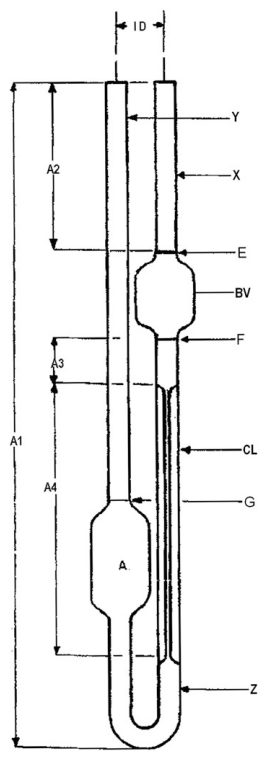
\includegraphics[height=0.4\paperheight]{figures/Ostwald_pruhledny.png}
        \caption{A - zásobní nádoba;\\G - plnicí ryska;\\CL - kapilára;\\E,F - měřicí rysky;\\BV - měřicí baňka.}
        \label{sfig:Ostwald_normalni}
    \end{subfigure}
    \begin{subfigure}[b]{.3\textwidth}
        \captionsetup{justification=centering}
        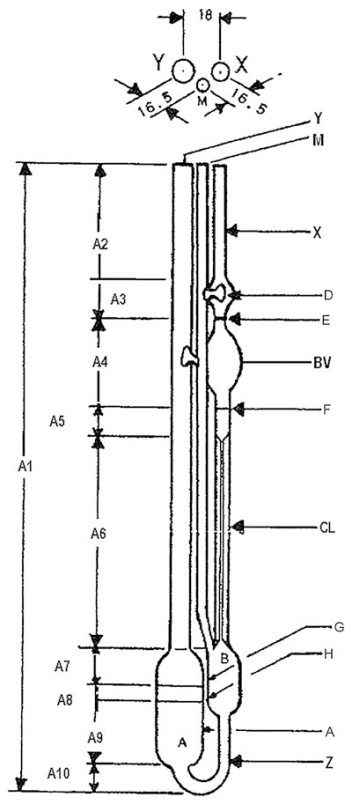
\includegraphics[height=0.4\paperheight]{figures/ubbelohde.png}
        \caption{A - zásobní nádoba;\\G,H - plnicí rysky;\\CL - kapilára;\\E,F - měřicí rysky;\\BV - měřicí baňka.}
        \label{sfig:Ubbelohde}
    \end{subfigure}
    \caption{Ostwaldův viskozimetr pro neprůhledné kapaliny (vlevo), Ostwaldův viskozimetr pro průhledné kapaliny (uprostřed) a~Ubbelohdeho viskozimetr (vpravo).~\cite{book:Calibration_of_viscometers}}
    \label{fig:viskozimetry}
\end{figure} %Viskozimetry

\paragraph{Ostwaldův viskozimetr pro průhledné kapaliny:}
Tento viskozimetr je znázorněn na obrázku \ref{sfig:Ostwald_normalni}, jednotlivé části přístroje budou popisovány písmeny z~tohoto obrázku. Viskozimetr je umístěn (ideálně ve vodní lázni) do stojanu a~je ověřena jeho svislá poloha. Měřená kapalina je do přístroje umístěna pomocí pipety plnicí trubicí (Y) tak, aby její hladina v~zásobní nádobě (A) po ustálení byla v~úrovni plnicí rysky (G). Po ustálení hladin a~teploty je na měřicí trubici (X) nasazen pipetovací balónek a~kapalina vysáta tak, aby její hladina v~měřicí trubici (X) přesáhla měřicí rysku (E) o~přibližně \SI{5}{\milli\metre}.\footnotemark Plnicí trubice (Y) může být zazátkována. Následně je pipetovací balónek odstraněn (to platí i~pro případnou zátku): kapalina v~tento okamžik začíná téct. Měření času je započato v~momentě, kdy meniskus kapaliny v~měřicí trubici (X) projde první měřicí ryskou (E) a~ukončeno v~momentě, kdy meniskus projde druhou měřicí ryskou (F).~\cite{book:Calibration_of_viscometers}
\footnotetext{Tato metoda sání kapaliny není vhodná pro těkavé látky. Pro těkavé látky je lepší nasadit pipetovací balónek na plnicí trubici (Y) a~kapalinu nad měřicí rysku (E) vytlačit přetlakem.}

\paragraph{Ostwaldův viskozimetr pro neprůhledné kapaliny:}
\label{sec:zpetny_ostwald}
Tento viskozimetr je znázorněn na obrázku~\ref{sfig:Ostwald_zpetny}, jednotlivé části přístroje budou popisovány písmeny z~tohoto obrázku. Viskozimetr je umístěn (ideálně ve vodní lázni) do stojanu a~je ověřena jeho svislá poloha. Měřená kapalina je vlita do zásobní nádoby (X) tak, aby se meniskus hladiny dostal na plnicí rysku (I). Poté je měřicí trubice (Y) uzavřena zátkou. Následně je do zásobní nádoby (X) dolit zbytek kapaliny tak, aby se hladina kapaliny v~zásobní nádobě (X) dostala na úroveň plnicí rysky (H). Po ustálení teploty je zátky z~měřicí trubice (Y) odstraněna: kapalina začíná téct. Měření času je započato v~momentě, kdy meniskus kapaliny v~měřicí trubici (Y) projde první měřicí ryskou (E) a~ukončeno v~momentě, kdy meniskus projde druhou měřicí ryskou (F).~\cite{book:Calibration_of_viscometers}

\paragraph{Ubbelohdeho viskozimetr:} Tento viskozimetr je znázorněn na obrázku \ref{sfig:Ubbelohde}, jednotlivé části přístroje budou popisovány písmeny z~tohoto obrázku. Hlavní odlišností tohoto typu viskozimetru od viskozimetru dle Ostwalda je ten, že během měření dojde k~přetržení kapalinového sloupce. Zároveň má trubici (M), která slouží k~vyrovnání tlaků pod a~nad kapilárou. Tyto dva aspekty zajišťují výhodu Ubbelohdeho viskozimetru: rozdíl tlaku nezávisí na naplnění zásobní nádoby (A) a~přesnost naplnění viskozimetru tím pádem neovlivňuje výsledky měření.~\cite{wiki:Ubbelohde_viscometer} Samotné měření pak probíhá takto: měřená kapalina je nalita plnicí trubicí (Y) do zásobní nádoby (A) tak, aby se hladina kapaliny po ustálení nacházela mezi plnicími ryskami (G) a~(H). Poté je vyrovnávací trubice (M) ucpána zátkou nebo prstem, na měřicí trubici (X) je nasazen pipetovací balónek a~měřená kapalina je do měřicí trubice (X) vysáta tak, aby meniskus její hladiny přesahoval měřicí rysku (E) o~zhruba \SI{5}{\milli\metre}. Otvor vyrovnávací trubice (M) je uvolněn. Následně je odstraněn pipetovací balónek (případně jiný zdroj sání) z~měřicí trubice (X): kapalina začíná téct. Měření času je započato v~momentě, kdy meniskus kapaliny v~měřicí trubici (X) projde první měřicí ryskou (E) a~ukončeno v~momentě, kdy meniskus projde druhou měřicí ryskou (F).~\cite{book:Calibration_of_viscometers}

%%%%%%%%%%%%%%%%%%%%%%%%%%%%%%%%%%%%%%%%%%%%%%%%%%%%%%%%%%%%%%%%%%%%%%
\subsection{Nálevkové viskozimetry}%%%%%%%%%%%%%%%%%%%%%%%%%%%%%%%%%%%
%%%%%%%%%%%%%%%%%%%%%%%%%%%%%%%%%%%%%%%%%%%%%%%%%%%%%%%%%%%%%%%%%%%%%%

Nálevkové viskozimetry pracují, stejně jako kapilární viskozimetry, na principu měření času. V~zásadě se tedy také řídí Hagenovým-Poiseulleovým zákonem, který byl popsán na straně~\pageref{sec:tečení_trubicí} a~následujících. Viskozimetr se sestává z~nádoby (většinou ve tvaru kelímku nebo nálevky), která má ze spodní strany otvor o~přesně stanoveném průměru. Nádoba se ponoří do měřené kapaliny, počká se, až se zcela naplní měřenou kapalinou, poté se z~kapaliny vyjme a~měří se čas, za který kapalina z~nádoby vyteče (tj.~až do prvního přerušení proudu). Tento čas lze pomocí vztahu podobnému tomu, který platí pro kapilární viskozimetry (str.~\pageref{eq:kapilarni_viskozimetr}), přepočítat na kinematickou viskozitu měřené kapaliny. Výpočetní vztahy se mění v~závislosti na viskozimetru a~většinou je stanovuje výrobce. Obecně platí vztah:~\cite{Article:Rapid_and_economic_chocolate_viscosity}
\begin{equation}
    \nu = K(t-c)\text{,}
\end{equation}
kde $\nu$ je kinematická viskozita měřené kapaliny, $t$ je čas průtoku nálevkovým viskozimetrem a~$K$ a~$c$ jsou přístrojové konstanty (určené výrobcem).
\par\noindent
Konstrukcí nálevkových viskozimetrů existuje celá řada. Liší se většinou tvarem, některé se také neplní ponořením. Některé konstrukce nálevkových viskozimetrů si čtenář může prohlédnout na obrázku \ref{fig:nalevkove_viskozimetry}.
\par\noindent
Zásadní nevýhody tohoto typu viskozimetru jsou chybějící tepelná regulace a~fakt, že hydrostatický tlak se v~průběhu měření z~důvodu vytékání kapaliny postupně mění. Jsou tedy oproti ostatním druhům viskozimetrů méně přesné. Jejich výhodou je nízká cena, dobrá dostupnost, jednoduché a~časově nenáročné použití.

\begin{figure}
    \begin{subfigure}[b]{.3\textwidth}
        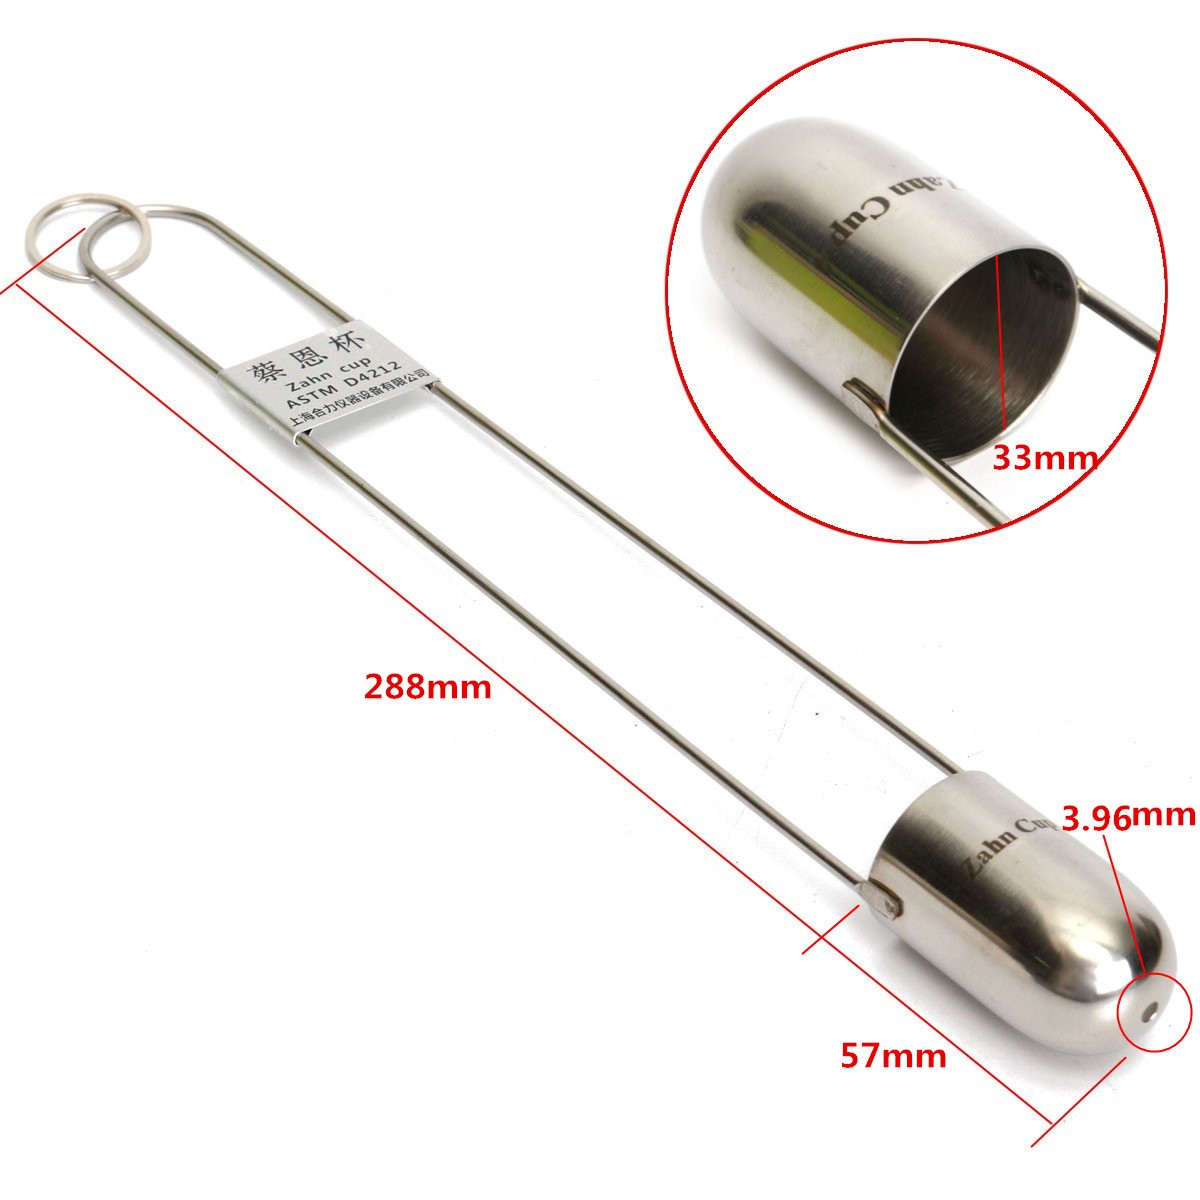
\includegraphics[width = \linewidth]{figures/zahn cup viscometer.jpg}
        \caption{Viskozimetr dle Zahna.~\cite{Figure:zahn_cup_viscometer}}
    \end{subfigure}
    \hfill
    \begin{subfigure}[b]{.3\textwidth}
        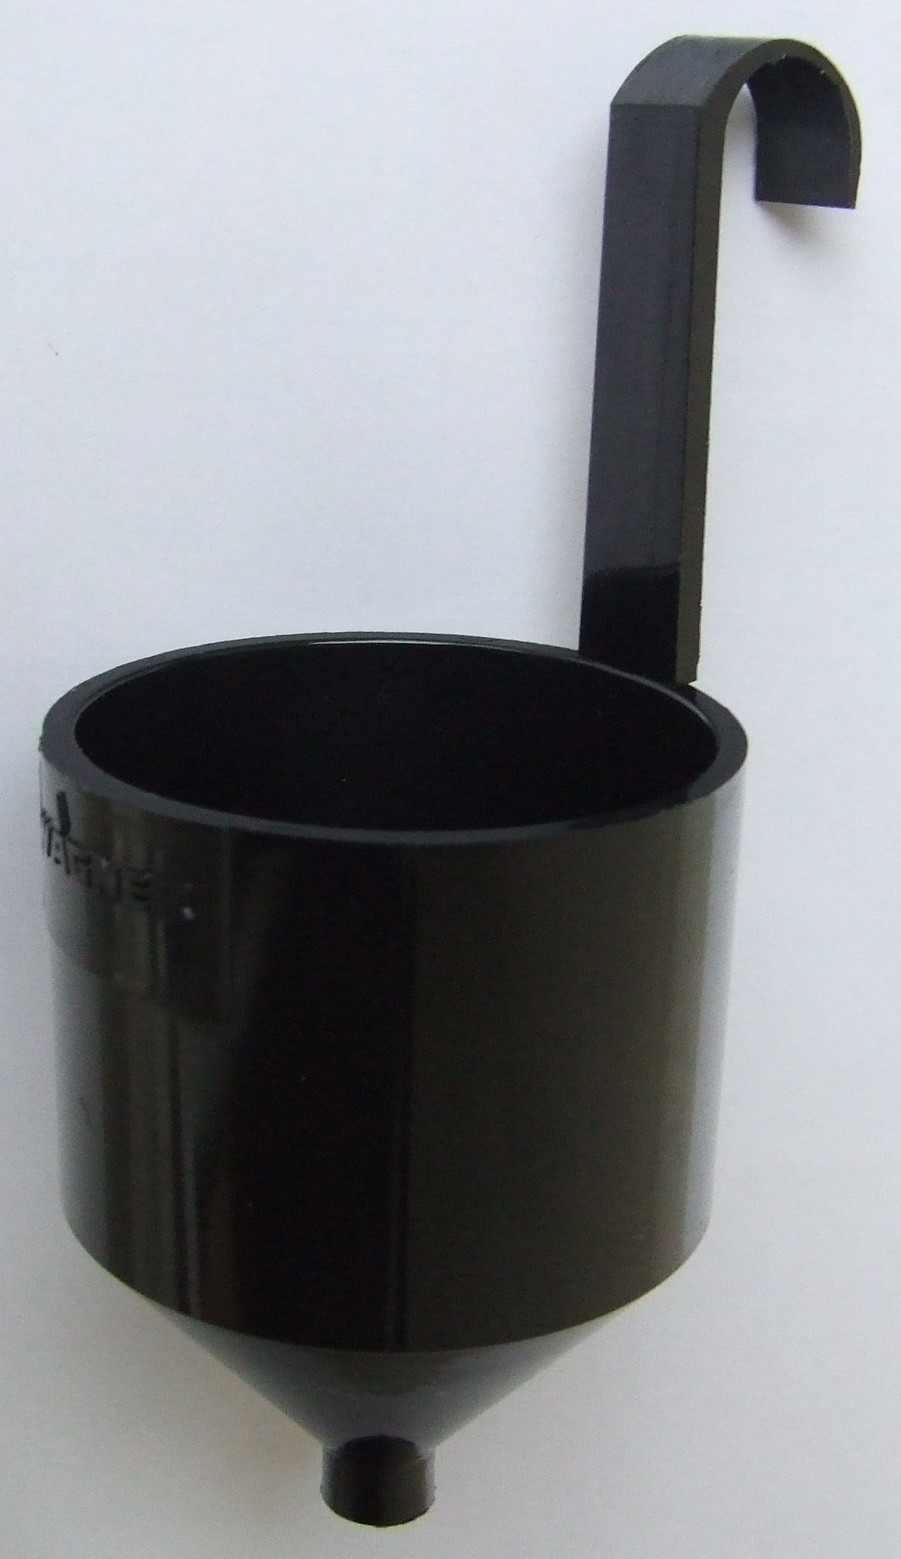
\includegraphics[width = \linewidth]{figures/ford cup viscometer.jpg}
        \caption{Viskozimetr dle Forda.~\cite{Figure:ford_cup_viscometer}}
    \end{subfigure}
    \hfill
    \begin{subfigure}[b]{.3\textwidth}
        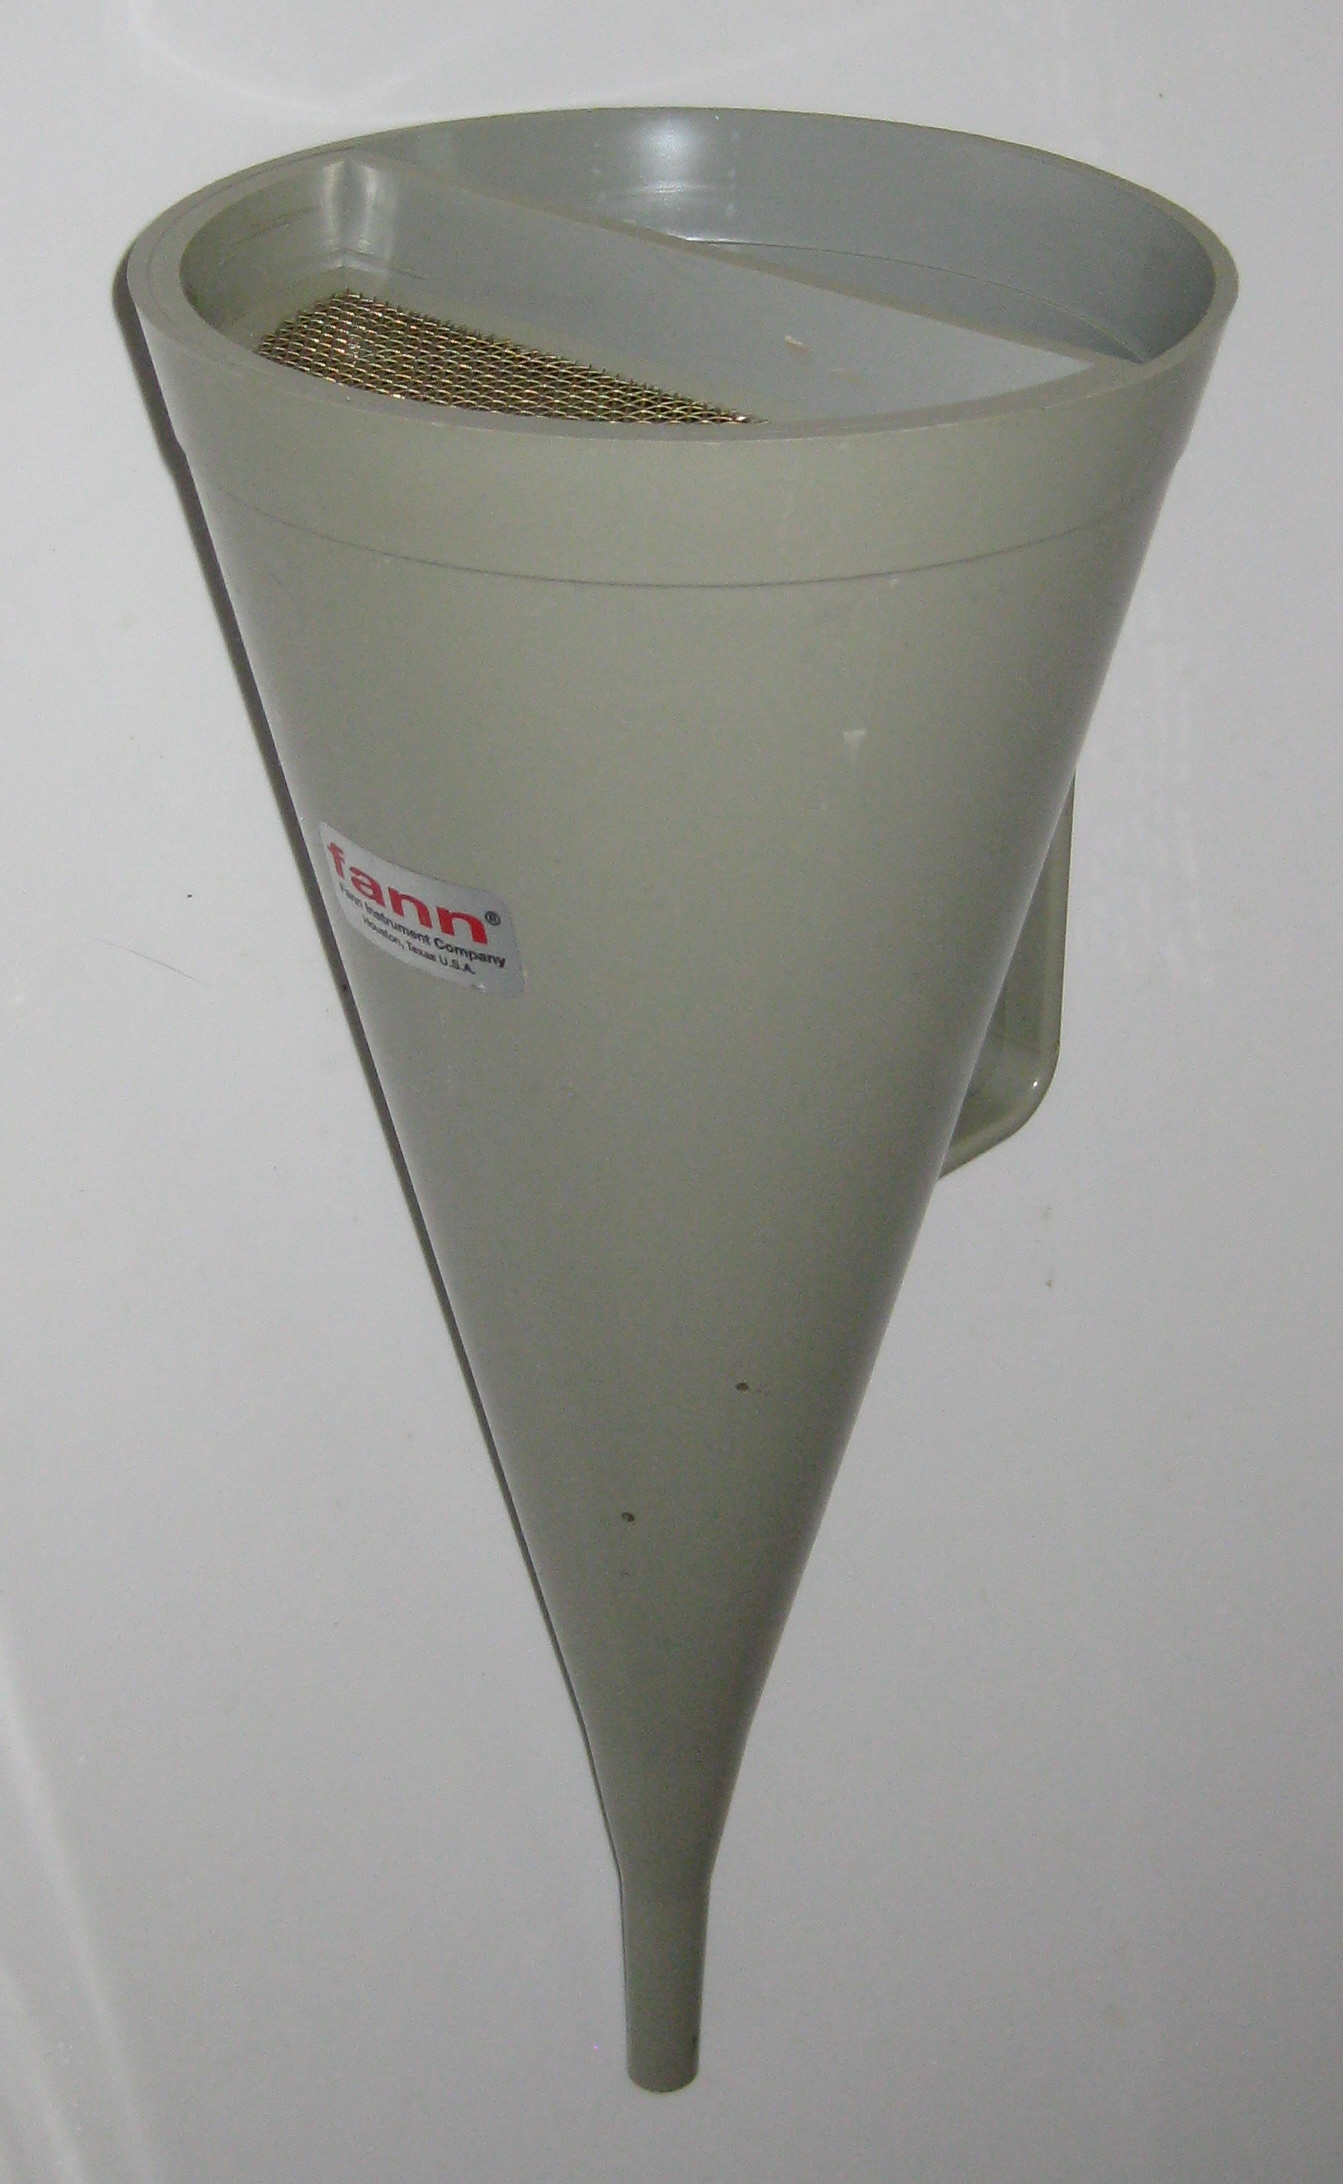
\includegraphics[width = \linewidth]{figures/Marsh_funnel.jpg}
        \caption{Viskozimetr dle Marshe.~\cite{Figure:marsh_funnel}}
    \end{subfigure}
    \caption{Různé typy nálevkových viskozimetrů.}
    \label{fig:nalevkove_viskozimetry}
\end{figure}

%%%%%%%%%%%%%%%%%%%%%%%%%%%%%%%%%%%%%%%%%%%%%%%%%%%%%%%%%%%%%%%%%%%%%%
\subsection{Tělískové viskozimetry}%%%%%%%%%%%%%%%%%%%%%%%%%%%%%%%%%%%
%%%%%%%%%%%%%%%%%%%%%%%%%%%%%%%%%%%%%%%%%%%%%%%%%%%%%%%%%%%%%%%%%%%%%%

Tělískové viskozimetry pracují na principu měření rychlosti, kterou je těleso schopno pohybovat se kapalinou, pokud je hnáno silou známé velikosti. Hnací silou ne nejčastěji síla tíhová, takové viskozimetry se pak nazývají \emph{pádové}. Nejčastěji používanými tělísky jsou tělíska kulového tvaru (viskozimetry používající kulová tělíska se pak nazývají \emph{kuličkové}).\footnotemark Rychlost pohybu (pádu) tělíska je zjišťována pomocí měření času, za který tělísko propadne mezi dvěma hladinami, jejichž vzdálenost je známá. Teoretický princip fungování pádového kuličkového viskozimetru bude popsán níže.
\footnotetext{Dalším oblíbeným tvarem tělíska je válcový píst.}

\subsubsection{Teoretické poznatky, Stokesův zákon}%%%%%%%%%%%%%%%%%%%

Představme si kouli, která rovnoměrně padá kapalinou. Výslednice všech sil působících na takovou kouli musí být nulová. Síly, které na kouli působí, jsou:
\begin{itemize}[noitemsep, topsep = 0pt]
    \item \underline{Tíhová síla} $\vec{F}_g$, působící dolů,
    \item \underline{Vztlaková síla} $\vec{F}_{vz}$, působící nahoru, a~    \item \underline{\smash{Odporová síla}} $\vec{F}_\eta$, působící proti směru pohybu, tj.~nahoru.\footnote{Při měření viskozity velmi hustých kapalin se může stát, že vztlaková síla přesáhne sílu tíhovou. Tělísko se pak pohybuje směrem vzhůru a~ve všech vztazích níže je pak nutné počítat se zápornou pádovou rychlostí $v$.}
\end{itemize}
Platí tedy:
\begin{equation}
    \vec{F}_g + \vec{F}_{vz} + \vec{F}_\eta = 0\text{.}
\end{equation}
Velikosti $\vec{F}_{vz}$ a~$\vec{F}_\eta$ musí dohromady dát velikost $\vec{F}_g$: směry vektorů tedy nebudeme dále uvažovat a~budeme počítat:
\begin{equation}
    F_g = F_{vz} + F_\eta\text{.}
\end{equation}
Víme, že:
\begin{align}
    \begin{split}
        F_g &= mg\text{,}\\
        F_{vz} &= V\rho g\text{,}
    \end{split}
\end{align}
kde $m$ je hmotnost koule, $V$ je objem vytlačené kapaliny, zde tedy objem koule, $\rho$ je hustota kapaliny a~$g$ je tíhové zrychlení. Pro velikost odporové síly $F_\eta$ platí tzv.~\emph{Stokesův zákon}:~\cite{book:Calibration_of_viscometers}\cite{wiki:Stokes_law}
\begin{equation}
    F_\eta = 6\pi r\eta v\text{,}
\end{equation}
kde $r$ je poloměr koule, $\eta$ je dynamická viskozita tekutiny a~$v$ je rychlost pohybu koule skrz kapalinu.\footnotemark Dohromady tedy platí:
\footnotetext{Tento zákon platí pouze pro malá Reynoldsova čísla, tj.~pro laminární obtékání koule a~malé rychlosti.}
\begin{equation}
    mg = V\rho g + 6\pi r\eta v\text{.}
\end{equation}
Dosadíme $m = V\rho_k$, kde $\rho_k$ je hustota koule (a $\rho_t$ bude dále hustota tekutiny), a~$V = \frac{4}{3}\pi r^3$. Dostáváme:
\begin{equation}
    \frac{4}{3}\pi r^3 \rho_k g = \frac{4}{3}\pi r^3 \rho_t g + 6\pi r\eta v\text{,}
\end{equation}
a pro viskozitu kapaliny $\eta$ tedy platí:~\cite{book:Calibration_of_viscometers}
\begin{equation}
    \eta = \frac{2r^2g(\rho_k-\rho_t)}{9v}\text{,}
\end{equation}
a pokud $v = \frac{\Delta h}{t}$, kde $\Delta h$ je dráha, kterou padající koule urazí za čas $t$, je možné psát:
\begin{equation}
    \eta = \frac{2r^2gt(\rho_k-\rho_t)}{9\Delta h}\text{,}
    \label{eq:kulickovy_viskozimetr}
\end{equation}
kde čas $t$ je jediná proměnná (a tedy měřená) veličina.

\subsubsection{Konstrukce a~použití}%%%%%%%%%%%%%%%%%%%%%%%%%%%%%%%%%%

Konstrukcí, které využívají výše uvedený princip, je celá řada. Existují komerčně prodávané kuličkové viskozimetry, většinou si však každý konkrétní výzkum upraví aparaturu dle vlastních potřeb. Hrubou představu o~konstrukci kuličkového viskozimetru si může čtenář udělat z~obrázku \ref{fig:kuličkový_viskozimetr}.
\par\noindent
Viskozimetr jako takový tvoří skleněná trubice, do které je obsluhou přístroje vhazováno kulové tělísko. Měřicí trubice je umístěna ve vodní lázni, aby bylo možné regulovat teplotu měřené kapaliny. Teplota lázně je kontrolována teploměrem. Na měřicí trubici bývají vyznačeny rysky: měřen je čas mezi průchodem tělíska první a~druhou ryskou. K~výpočtu viskozity je pak použit vztah \ref{eq:kulickovy_viskozimetr} s~tím, že v~reálných případech musí být připočten korekční faktor (válec, ve kterém se tělísko pohybuje, není nekonečně široký, a~obtékání tělíska je tedy oproti Stokesovu zákonu ovlivňováno).
\par\noindent
Je evidentní, že tělískový viskozimetr takovéto konstrukce je použitelný pouze pro průhledné kapaliny. Pro neprůhledné kapaliny se konstruují viskozimetry, které detekují pohyb tělíska pomocí cívek umístěných okolo přístroje nebo jiným technicky náročným způsobem.~\cite{thesis:vysokotlaky_viskozimetr}
\begin{figure}
    \centering
    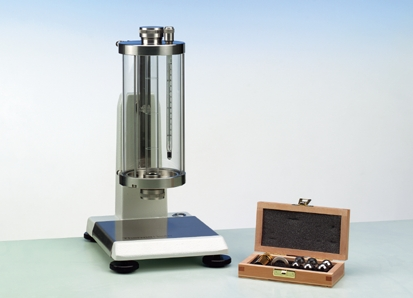
\includegraphics[width = 0.75\linewidth]{figures/kuličkový viskozimetr.jpg}
    \caption{Kuličkový viskozimetr.~\cite{Figure:kulickovy_viskozimetr}}
    \label{fig:kuličkový_viskozimetr}
\end{figure}

%%%%%%%%%%%%%%%%%%%%%%%%%%%%%%%%%%%%%%%%%%%%%%%%%%%%%%%%%%%%%%%%%%%%%%
\subsection{Rotační viskozimetry}%%%%%%%%%%%%%%%%%%%%%%%%%%%%%%%%%%%%%
%%%%%%%%%%%%%%%%%%%%%%%%%%%%%%%%%%%%%%%%%%%%%%%%%%%%%%%%%%%%%%%%%%%%%%

Všechny výše popsané měřicí metody jsou vhodné pouze k~měření viskozity newtonovských kapalin, jelikož není možné zjistit, při jakém tečném napětí nebo rychlosti deformace měření probíhá. Tento problém je řešitelný konstrukcí rotačního viskozimetru.
\par\noindent
Rotační viskozimetry, podobně jako tělískové viskozimetry, měří odpor kladený tělesu, které se pohybuje v~kapalině. Konkrétně je do kapaliny umístěno těleso, které se otáčí kolem své osy, a~je měřen moment síly, kterým musí být na těleso působeno, aby v~tomto otáčivém pohybu setrvalo. Tato rotační tělesa mají většinou tvar válce a~nazývají se \emph{měřicí vřetena}.

\subsubsection{Teoretické poznatky}%%%%%%%%%%%%%%%%%%%%%%%%%%%%%%%%%%%

Uvažujme válcovou nádobu o~poloměru $R$, která je naplněna kapalinou. Dále uvažujme válec o~poloměru $R_v$ a~výšce $h$, který je ponořený v~této kapalině s~tím, že jeho osa je kolmá na hladinu kapaliny a~je tedy totožná s~osou nádoby. Konečně uvažujme, že tento válec se kolem své osy otáčí úhlovou rychlostí $\Omega$. Kapalina přiléhající k~plášti válce se bude otáčet spolu s~válcem rychlostí $\Omega$, kapalina přiléhající ke stěně nádoby se nebude pohybovat vůbec. Existuje zde tedy gradient úhlové rychlosti kapaliny $\frac{\dd\omega}{\dd r}$, jelikož $\omega(R_v) = \Omega$ a~$\omega(R) = 0$.\label{eq:Uhlova_rychlost} Z~Newtonova zákona viskozity (vztah~\ref{eq:Newtonův zákon viskozity}, str.~\pageref{eq:Newtonův zákon viskozity}) víme, že $\tau = \eta\dot\gamma$. Gradient rychlosti $\frac{\dd v}{\dd r}$ lze získat vztahem (viz str.~\pageref{eq:gamma_gradient}):
\begin{equation}
    \dot\gamma = -\frac{\dd v}{\dd r} = -r\frac{\dd\omega}{\dd r}\text{.}
\end{equation}
Platí tedy, že smykové napětí působící na plášť válce o~poloměru $r$ je rovno:
\begin{equation}
    \tau = -\eta r\frac{\dd\omega}{\dd r}\text{.}
\end{equation}
Podobně jako v~kapitole o~kapilárních viskozimetrech (str.~\pageref{eq:gamma_gradient}), i~zde budeme uvažovat, že kapalina je ve skutečnosti tvořena nekonečným množstvím nekonečně tenkých válců. Situace je tedy podobná jako na obr.~\ref{fig:valce}, ale osa válců je svislá (kolmá na hladinu kapaliny).
Ze vztahu~\ref{eq:hook_smyk} zároveň víme, že $\tau = \frac{F}{S'}$. Plochu $S'$ zde tvoří plášť válce, takže platí $S' = 2\pi rh$. Dohromady platí:
\begin{equation}
    \frac{F}{2\pi rh} = -\eta r\frac{\dd\omega}{\dd r}\text{.}
\end{equation}

\begin{figure}[h!]
    \centering
    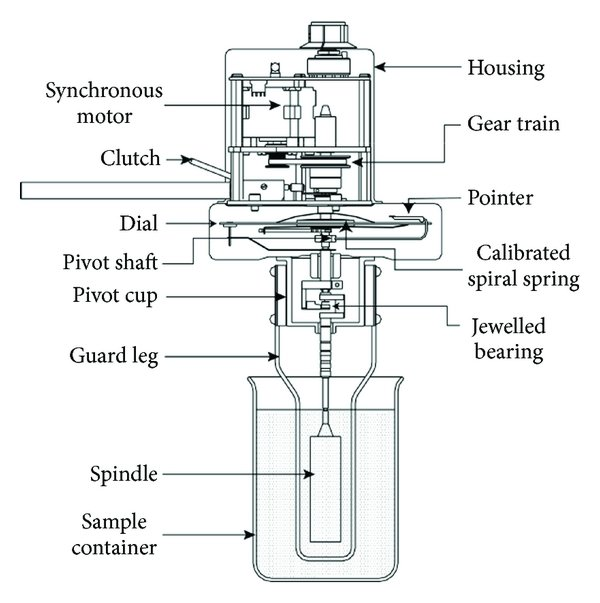
\includegraphics[width = 0.6\linewidth]{figures/brookfield.png}
    \caption{Schéma jedné konkrétní (poměrně komplikované) konstrukce viskozimetru dle Brookfielda.~\cite{Figure:Brookfield}}
    \label{fig:brookfield}
\end{figure}

Síla $F$ působící na plášť infinitezimálního válce má tedy velikost:~\cite{book:Calibration_of_viscometers}
\begin{equation}
    F = -2\pi r^2h\eta\frac{\dd \omega}{\dd r}\text{.}
\end{equation}
Pro moment síly platí $M = F\cdot d$, kde $F$ je síla a~$d$ je rameno síly. Rameno síly je zde rovno poloměru infinitezimálního válce, a~pro moment síly $\dd M$ působící na něj tedy platí:
\begin{equation}
    \dd M = -2\pi r^3h\eta\frac{\dd \omega}{\dd r}\text{.}
\end{equation}
Moment působící na skutečný ponořený válec je pak součtem všech těchto malých momentů $\dd M$. Integrováním vzhledem k~$r$ získáváme:\footnotemark~\cite{book:Calibration_of_viscometers}\cite{Article:barr}
\begin{equation}
    M = 4\pi h\eta\Omega\frac{R^2R_v^2}{R^2-R_v^2}\text{.}
    \label{eq:moment_viskozimetr}
\end{equation}
\footnotetext{Samotnému mi princip této integrace není plně objasněn. Při pokusném integrování na papíře jsem dospěl k~jinému výsledku. Vyzývám tedy čtenáře, aby se o~integraci pokusil sám: možná dospěje k~rozumnému závěru.}
Rychlost deformace ve vzdálenosti $r$ od osy válce lze spočítat vztahem:~\cite{material:brookfield_viscometers}
\begin{equation}
    \dot\gamma(r) = \frac{2\Omega R^2R_v^2}{r^2(R^2-R_v^2)}\text{.}
    \label{eq:viskozimetr_gamma}
\end{equation}
\begin{comment}
\begin{equation}
    M = \int_{R_v}^R-2\pi r^3h\eta\frac{\dd \omega}{\dd r}\dd r = -2\pi h\eta\int_{R_v}^Rr^3\frac{\dd \omega}{\dd r}\dd r\text{.}
\end{equation}
Tady tady proces na chvilku zastavíme a~budeme se věnovat otázce, kolik je $\int r^3\frac{\dd\omega}{\dd r}\dd r$. Integrací získáme:
\begin{equation}
    \int r^3\frac{\dd\omega}{\dd r}\dd r = \frac{r^4}{4}\cdot\omega(r)\text{.}
\end{equation}
Vzhledem k~tomu, že hodnoty $\omega(R_v)$ a~$\omega(R)$ jsou nám známé (viz úvod této podkapitoly, str. \pageref{eq:Uhlova_rychlost}), dospíváme k~závěru integrace:
\begin{equation}
    M = \frac{1}{2}\pi h\eta\Omega R_v^4\text{.}
\end{equation}

----- Chybný postup:
\par
Nyní musíme vyjádřit funkci úhlové rychlosti $\omega $~v závislosti na vzdálenosti od osy nádoby (poloměru infinitezimálního válce) $r$. Tato funkce je zde nazvána $\omega(r)$. V~úvodu této podkapitoly (str. \pageref{eq:Uhlova_rychlost}) jsou popsány dva body této funkce: $\omega(R_v) = \Omega$ a~$\omega(R) = 0$. Uvažme, že se v~zásadě jedná o~Couettovo proudění (viz str. \pageref{sec:Couettovo_proudění}), a~tedy bude úhlová rychlost klesat lineárně se zvyšující se vzdáleností od středu otáčení. Bude tedy platit $\omega = ar+b$ musíme jen zjistit hodnoty konstant $a$ a~$b$. Toto je případ lineární funkce určené dvěma body, konkrétně body $[R_v,\Omega]$ a~$[R,0]$. Platí pak:
\begin{equation}
    a~= \frac{\Omega}{R_v-R};\: b = -\frac{\Omega R}{R_v-R}
\end{equation}
Dosazením zpět do lineární rovnice dostáváme:
\begin{equation}
    \omega(r) = \Omega\frac{r-R}{R_v-R} = \Omega\frac{(r-R)(R_v+R)}{R_v^2-R^2}
\end{equation}

Dosazením do lineární rovnice získáváme:
\begin{align}
    \begin{split}
        \omega(r) &= \frac{\Omega r}{R_v-R} + \Omega +\frac{\Omega R_v}{R_v-R} = \frac{\Omega(R_v+r)}{R_v-R}+\frac{\Omega(R_v-R)}{R_v-R} = \frac{\Omega(r+2R_v-R)}{R_v-R} =\\
        &= \Omega\frac{(r+2R_v-R)(R_v+R)}{(R_v-R)(R_v+R)} = \Omega\frac{R_v(r + 2R_v + R) + Rr -R^2}{R_v^2 - R^2}\text{.}
    \end{split}
\end{align}
Pro moment $M$ tedy platí:
\begin{equation}
    M = -2\pi h\eta\int_{R_v}^Rr^3\frac{\dd \omega}{\dd r}\dd r = -2\pi h\eta\Omega\cdot\left(\frac{2R_vR^4(R_v + R) - R_v^5(3R_v + 2R) + R_v^4R^2}{4(R_v^2 - R^2)}\right)
\end{equation}
\end{comment}

\subsubsection{Konstrukce a~použití}%%%%%%%%%%%%%%%%%%%%%%%%%%%%%%%%%%

Stejně jako u~všech ostatních druhů viskozimetrů, i~rotačních viskozimetrů existuje několik konstrukcí. Mezi vynálezci jedné z~nich uveďme např.~Maurice Couetta, jehož jméno už v~této práci zaznělo.~\cite{wiki:Maurice_Couette} Nás však budou zajímat viskozimetry dle Brookfielda, jelikož viskozimetr této konstrukce bude později v~této práci použit k~měření viskozity čokolády.
\par\noindent
Rotační viskozimetr dle Brookfielda využívá k~měření viskozity měřicí vřeteno válcového tvaru, které rotuje kolem své osy symetrie a~jehož osa rotace je totožná s~osou nádoby, ve které se nachází měřená kapalina. Přístroj měří moment síly, který je nutný k~udržení válce v~rovnoměrném otáčivém pohybu, vyjádřený vztahem~\ref{eq:moment_viskozimetr}.
\par\noindent
Měřicí vřeteno je poháněno motorem v~přístroji. Vřeteno však není spojeno s~motorem přímo: motor je spojen s~ručkou přístroje, kterou vychyluje. Ručka přístroje je s~měřicím vřetenem spojena pomocí spirálové pružiny. Velikost deformace pružiny je pak přímo úměrná momentu síly.~\cite{man:brookfield} Diagram poměrně složité konstrukce viskozimetru dle Brookfielda je na obrázku \ref{fig:brookfield}.

%%%%%%%%%%%%%%%%%%%%%%%%%%%%%%%%%%%%%%%%%%%%%%%%%%%%%%%%%%%%%%%%%%%%%%
\newpage%%%%%%%%%%%%%%%%%%%%%%%%%%%%%%%%%%%%%%%%%%%%%%%%%%%%%%%%%%%%%%
\section{Čokoláda}%%%%%%%%%%%%%%%%%%%%%%%%%%%%%%%%%%%%%%%%%%%%%%%%%%%%
%%%%%%%%%%%%%%%%%%%%%%%%%%%%%%%%%%%%%%%%%%%%%%%%%%%%%%%%%%%%%%%%%%%%%%
%%%%%%%%%%%%%%%%%%%%%%%%%%%%%%%%%%%%%%%%%%%%%%%%%%%%%%%%%%%%%%%%%%%%%%

Čokoláda je oblíbená pochutina vyráběná ze semen kakaovníku (\emph{Theobroma cacao}, což mimochodem v~překladu znamená \emph{potrava bohů}).~\cite{wiki:Kakao} Vyrábí se z~ní celá řada dalších produktů.

%%%%%%%%%%%%%%%%%%%%%%%%%%%%%%%%%%%%%%%%%%%%%%%%%%%%%%%%%%%%%%%%%%%%%%
\subsection{Složení čokolády}%%%%%%%%%%%%%%%%%%%%%%%%%%%%%%%%%%%%%%%%%
\label{sec:složení_čokolády}%%%%%%%%%%%%%%%%%%%%%%%%%%%%%%%%%%%%%%%%%%

Čokoláda je (ve svém kapalném skupenství) suspenzí různých rozptýlených látek v~kakaovém másle. V~hořkých čokoládách tvoří rozpuštěné látky částečky kakaa (tzv.~kakaová sušina) a~cukr (sacharóza). V~mléčných čokoládách je kakaová složka částečně (ne však úplně) nahrazena mléčnou sušinou. V~bílé čokoládě se kakaová sušina vůbec nevyskytuje, jedinou složkou vyráběnou z~kakaa pak zůstává kakaové máslo, které drží ostatní složky (sacharózu, sušené mléko, lecitin a~většinou vanilku nebo vanilin) pohromadě. Hlavní složkou čokolády, ve které jsou všechny ostatní složky rozptýlené, však vždy zůstává kakaové máslo. Jeho vlastnosti jsou tedy naprosto zásadní a~budou popsány v~následujících kapitolách.~\cite{Article:chocolate_composition}\cite{Article:Determination_of_chocolate_viscosity}\cite{wiki:Chocolate}\cite{wiki:čokoláda}\cite{wiki:Bílá_čokoláda}

%%%%%%%%%%%%%%%%%%%%%%%%%%%%%%%%%%%%%%%%%%%%%%%%%%%%%%%%%%%%%%%%%%%%%%
\subsection{Reologické vlastnosti}%%%%%%%%%%%%%%%%%%%%%%%%%%%%%%%%%%%%
\label{sec:Reologické_vlastnosti_čokolády}%%%%%%%%%%%%%%%%%%%%%%%%%%%%

Popsat reologické vlastnosti čokolády není vůbec jednoduché.~\cite{Article:Determination_of_chocolate_viscosity} Obecně lze o~čokoládě tvrdit, že je (ve svém kapalném skupenství) pseudoplastickou (tedy nenewtonovskou) kapalinou.~\cite{Article:Comparison_of_models_chocolate}\cite{Article:Rapid_and_economic_chocolate_viscosity} Její chování se však do značné míry mění právě v~závislosti na tečném napětí, které v~čokoládě působí. Při vysokých tečných napětích se čokoláda chová jako newtonovská kapalina, naopak při velmi nízkých hodnotách tečného napětí neteče vůbec (a chová se tedy jako pevná látka). Zároveň se jedná o~kapalinu tixotropní.~\cite{Article:Determination_of_chocolate_viscosity}

\subsubsection{Binghamské látky}%%%%%%%%%%%%%%%%%%%%%%%%%%%%%%%%%%%%%%

Látkám, které začínají téci až od určitého tečného napětí říkáme \emph{plastické}.~\cite{material:Nenewtonovské_kapaliny}\cite{material:Viskozita_a_povrchove_napeti} Nejjednodušší formou plastické látky je tzv.~\emph{binghamská látka}. Pro ní platí, že se až do tečného napětí $\tau_0$ chová jako pevná látka (tj.~neteče a~chová se podle Hookeova zákona, viz str.~\pageref{sec:Hookeův_zákon}): toto napětí $\tau_0$ nazýváme \emph{prahové napětí}.~\cite{wiki:Bingham_plastic}\cite{material:Tokove_chovani_reologicke_modely} Od prahového napětí začíná binghamská látka téct a~vztah rychlosti deformace a~tečného napětí je při všech vyšších tečných napětích lineární (toková křivka je přímkou). Zdánlivá viskozita však s~rostoucím tečným napětím klesá, viz obr.~\ref{fig:apparent_viscosity}. Při limitním zvyšování tečného napětí (resp.~rychlosti deformace) k~nekonečnu získáváme hodnotu zdánlivé viskozity $\eta_\infty$ v~těchto krajních hodnotách. Pro popis chování binghamských látek pak platí vztah:~\cite{Article:Comparison_of_models_chocolate}\cite{Article:Extended_casson_equation}
\begin{equation}
    \tau = \tau_0 + \eta_B\cdot \dot\gamma\text{,}
    \label{eq:Bingham}
\end{equation}
kde $\tau_0$ je prahové napětí a~$\dot\gamma$ je rychlost deformace. $\eta_B$ je tzv.~\emph{binghamská viskozita}, pro kterou platí $\eta_B = \eta_\infty$. Binghamská viskozita $\eta_B$ je zároveň směrnicí přímky reogramu binghamské látky, jak je možné vidět na obrázcích~\ref{fig:apparent_viscosity} a~\ref{fig:rheology_diagram}.
\par\noindent
Jelikož se binghamské látky vyznačují právě onou lineární závislostí tečného napětí a~rychlosti deformace, není model popsaný vzorcem \ref{eq:Bingham} moc vhodný k~popisování vlastností čokolády, snad jen při vysokých tečných napětích, kdy se i~čokoláda projevuje spíše newtonovsky. Bude proto nutné tento model dále upravovat.

\subsubsection{Herschelovy–Bulkleyho tekutiny}%%%%%%%%%%%%%%%%%%%%%%%

Spojením Ostwaldovy-deWaaleovy rovnice (str.~\pageref{eq:ostwald_dewaale}) a~binghamského modelu získáváme vztah popisující tzv.~Herschelovu-Bulkleyho tekutinu:~\cite{Article:Comparison_of_models_chocolate}\cite{Article:Extended_casson_equation}
\begin{equation}
    \tau = \tau_0 + \eta_{pl}\cdot\dot\gamma^n\text{,}
\end{equation}
kde $\tau_0$ je opět prahové napětí látky, $\eta_{pl}$ je plastická viskozita tekutiny, $\dot\gamma$ je rychlost deformace a~pro $n$ viz kapitolu o~modelování nenewtonovských kapalin, str.~\pageref{eq:ostwald_dewaale}.
\par\noindent
Tento model je schopen popsat jak plastické, tak pseudoplastické vlastnosti kapaliny při relativně nízkých tečných napětích. Má však oproti modelu binghamských látek opačný problém: není schopen zachytit linearitu tokové křivky při vysokých tečných napětích. Odvážný čtenář si může dokázat, že pro Herschelův-Bulkleyho model platí:
\begin{equation}
    \lim_{\dot\gamma\to\infty} \frac{\dd\tau}{\dd\dot\gamma} = 0\text{,}
\end{equation}
a tento model tedy ani při vysokých hodnotách tečného napětí nemůže vyjadřovat lineární tokovou křivku. Je proto nutné vymyslet kompromisní model, který zachytí všechny tři důležité reologické vlastnosti čokolády, které byly popsány v~úvodu této kapitoly:
\begin{itemize}[noitemsep, topsep = 0pt]
    \item \underline{Plasticitu}, tedy tuhost čokolády při nízkých smykových napětích (a tedy existenci prahového napětí $\tau_0$),
    \item \underline{\smash{Pseudoplasticitu}} čokolády (tj.~nelinearitu její tokové křivky) při středních hodnotách smykových napětí, a~    \item \underline{Newtonovské chování} čokolády (tj.~linearitu její tokové křivky) při vysokých tečných napětích.
\end{itemize}

\subsubsection{Cassonův model}%%%%%%%%%%%%%%%%%%%%%%%%%%%%%%%%%%%%%%%%
\label{sec:Casson}

Tímto ideálním kompromisem je tzv.~\emph{Cassonův model}. Je vyjádřen vztahem:~\cite{Article:Comparison_of_models_chocolate}\cite{Article:Determination_of_chocolate_viscosity}\cite{Article:Extended_casson_equation}\cite{Article:Flow_properties_molten_chocolate}
\begin{equation}
    \sqrt{\tau} = \sqrt{\tau_{CA}} + \sqrt{\eta_{CA}\cdot\dot\gamma}\text{,}
    \label{eq:Casson_model}
\end{equation}
kde $\tau$ je tečné napětí, $\tau_{CA}$ je Cassonovo prahové napětí, $\eta_{CA}$ je Cassonova plastická viskozita, pro kterou platí $\eta_{CA} = \eta_\infty$ a~$\dot\gamma$ je rychlost deformace. Protože $\sqrt{\tau_{CA}}$ a~$\sqrt{\eta{CA}}$ jsou konstanty, můžeme se setkat i~se zápisem ve tvaru:~\cite{Article:Rapid_and_economic_chocolate_viscosity}
\begin{equation}
    \sqrt{\tau} = k_0 + k_1\cdot\sqrt{\dot\gamma}\text{,}
\end{equation}
kde $k_0 = \sqrt{\tau_{CA}}$ a~$k_1 = \sqrt{\eta_{CA}}$.
\par\noindent
Jelikož tento model obsahuje odmocniny, nemám, jak bych čtenáři naprosto intuitivně objasnil jeho fungování. Tento model však dobře popisuje všechny ze tří vlastností čokolády, které byly popsány výše, včetně lineárního průběhu tokové křivky při vysokých hodnotách tečného napětí: čtenář si opět může dokázat, že platí:
\begin{equation}
    \lim_{\dot\gamma\to\infty} \frac{\dd\tau}{\dd\dot\gamma} = \eta_{CA}\text{.}
\end{equation}
Pro nízké hodnoty tečného napětí lze Cassonův model aproximovat Herschelovým-Bulkleyho modelem (protože se zde neprojevuje linearita tokové křivky, kterou Herschelův-Bulkleyho model neumí vyjádřit). To jsem se pokusil zobrazit na obrázku~\ref{fig:Casson_vs_Herschel}.
\begin{figure}
    \centering
    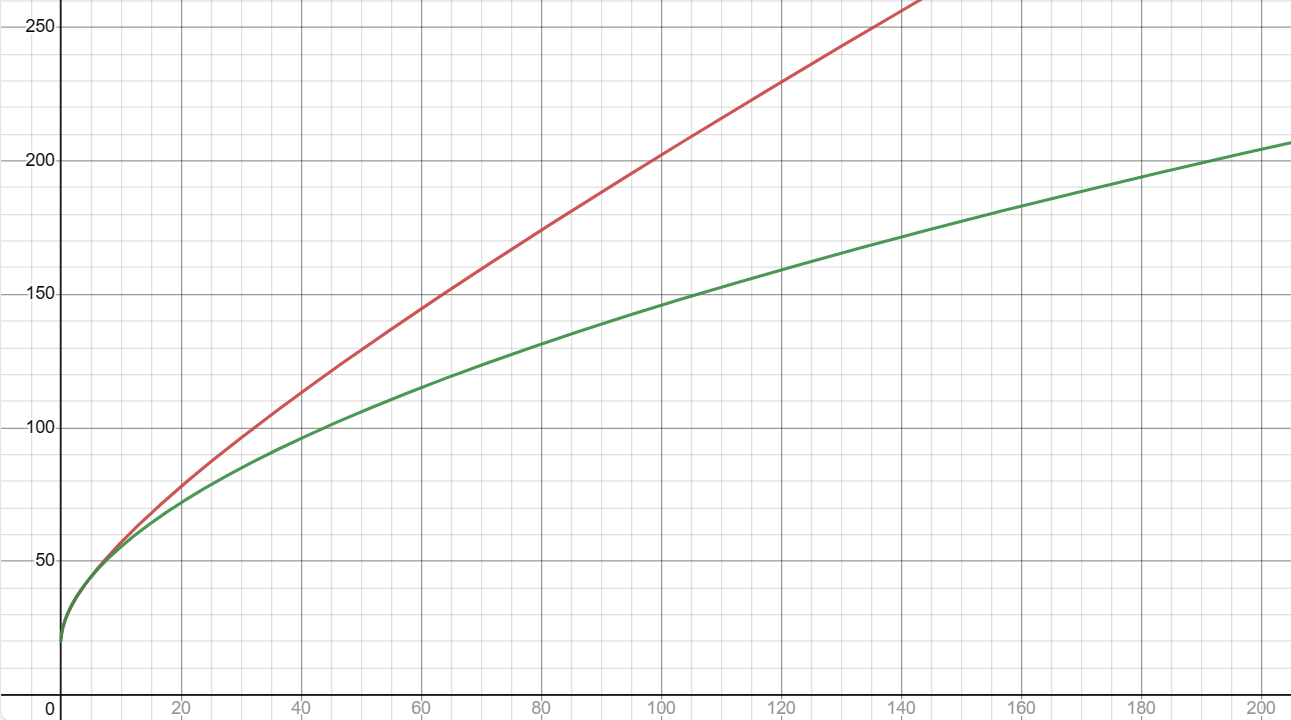
\includegraphics[width=\linewidth]{figures/Casson vs Herschel.png}
    \caption{Srovnání tokových křivek Cassonova modelu (červená křivka) s~Herschelovým-Bulkleyho modelem (zelená křivka) pro náhodně zadané hodnoty. Na ose $x$ je znázorněna rychlost deformace (zde bez jednotek) a~na ose $y$ tečné napětí (taktéž bez jednotek). Vidíme, že prahové napětí je $20$. Zároveň vidíme, že pro nízká tečná napětí je Herschelův-Bulkleyho model dobrou aproximací Cassonova modelu. Vytvořeno s~pomocí webové aplikace \url{desmos.com}.}
    \label{fig:Casson_vs_Herschel}
\end{figure}
\par\noindent
Pro své vlastnosti je Cassonův model základním modelem používaným cukrářskými organizacemi po celém světě.~\cite{Article:Determination_of_chocolate_viscosity} Přesto lze tento model dále vylepšovat různými korekčními faktory, aby se jeho výsledky lépe přiblížily skutečným vlastnostem čokolády.~\cite{Article:Determination_of_chocolate_viscosity} Při nízkých hodnotách tečného napětí se někteří uchylují k~používání tzv.~\emph{Carreau} modelu, který nebudu dále rozebírat, nebo jiných modelů.~\cite{Article:Flow_properties_molten_chocolate}\cite{material:Tokove_chovani_reologicke_modely}

%%%%%%%%%%%%%%%%%%%%%%%%%%%%%%%%%%%%%%%%%%%%%%%%%%%%%%%%%%%%%%%%%%%%%%
\subsection{Vlastnosti kakaového másla}%%%%%%%%%%%%%%%%%%%%%%%%%%%%%%%
%%%%%%%%%%%%%%%%%%%%%%%%%%%%%%%%%%%%%%%%%%%%%%%%%%%%%%%%%%%%%%%%%%%%%%

\subsubsection{Složení kakaového másla}%%%%%%%%%%%%%%%%%%%%%%%%%%%%%%%

Kakaové máslo tvoří triacylglyceroly esterifikované převážně dvěma nasycenými a~jednou nenasycenou mastnou kyselinou: kyselinou palmitovou (nasycená), stearovou (nasycená) a~olejovou (nenasycená). Každý triacylglycerol na sobě může mít navázanou jakoukoliv kombinaci (nejen) těchto mastných kyselin. Poměrné zastoupení jednotlivých triacylglycerolů v~kakaovém másle pak ovlivňuje vlastnosti čokolády.~\cite{Article:precrystallization}\cite{wiki:Triacylglycerol}

\subsubsection{Viskozita kakaového másla při jeho tuhnutí}%%%%%%%%%%%%

Při ochlazování kakaového másla dochází nejdříve ke krystalizaci triacylglycerolů, které jsou tvořené nasycenými mastnými kyselinami. Tím dochází k~rychlému zvýšení viskozity, kakaové máslo však zůstává v~kapalném skupenství, protože triacylglyceroly tvořené i~nenasycenými mastnými kyselinami krystalizují až při nižších teplotách: vzniká tedy suspenze\footnotemark. Triacylglyceroly tvořené třemi nasycenými mastnými kyselinami pak slouží jako krystalizační jádra pro další krystalizaci. Je však nutné podotknout, že příměsi v~čokoládě značně ovlivňují mechanismus krystalizace kakaového másla.~\cite{Article:precrystallization}
\footnotetext{Čokoláda je samozřejmě suspenzí tak či tak, jelikož jsou v~ní rozptýlené jiné látky popsané v~kapitole na str.~\pageref{sec:složení_čokolády}. Zde mluvíme o~samotném kakaovém másle.}

\subsubsection{Polymorfie a~bod tání}%%%%%%%%%%%%%%%%%%%%%%%%%%%%%%%%%
\label{sec:polymorfie}

Kakaové máslo je polymorfní látka.~\cite{Article:cocoa_butter_polymorphism} To znamená, že je schopné krystalizovat do několika krystalických struktur.~\cite{wiki:Polymorfie} Každá z~těchto krystalických struktur má odlišný bod tání. Body tání jednotlivých polymorfů kakaového másla jsou v~tabulce~\ref{tab:polymorfy}. Čokoláda se vyrábí tak, aby většina kakaového másla krystalizovala do polymorfu $\beta_2$.~\cite{Article:cocoa_butter_tempering} Čokoláda by ve stavu, ve kterém ji koupíme, měla mít bod tání mezi 30 a~\SI{35}{\degreeCelsius}.

\begin{table}
    \centering
    \begin{tabular}{|c|c|}
        \hline
        Polymorf & Rozsah bodu tání [\SI{}{\degreeCelsius}] \\\hline
        $\alpha$ & 17,1 -- 24,0\\
        $\beta_2'$ & 22,4 -- 28,0\\
        $\beta_1'$ & 21,0 -- 33,0\\
        $\beta_2$ & 30,0 -- 34,5\\
        $\beta_1$ & 33,5 -- 36,3\\
        \hline
    \end{tabular}
    \caption{Rozsahy bodů tání jednotlivých polymorfů kakaového másla.\cite{Article:cocoa_butter_polymorphism}}
    \label{tab:polymorfy}
\end{table}

Polymorf $\alpha$ krystalizuje do šesterečné, polymorfy $\beta_2'$ a~$\beta_1'$ do kosočtverečné a~polymorfy $\beta_2$ a~$\beta_1$ do trojklonné krystalografické soustavy.~\cite{Article:precrystallization}\cite{wiki:crystal_structure}
\par\noindent
Při tuhnutí z~kapalného skupenství však čokoláda krystalizuje pouze do polymorfů $\alpha$, $\beta_1'$ a~$\beta_2'$.~\cite{Article:molecular_polymorphism} Přetavená čokoláda má tedy nižší bod tání a~jiné reologické a~pevnostní vlastnosti než taková, která od výroby neroztála.\footnote{S tímto jevem se čtenář mohl setkat, pokud mu čokoláda někdy roztála třeba v~batohu nebo v~kapse.} Výrobní proces čokolády pak musí být navržen tak, aby došlo ke krystalizaci do polymorfu $\beta_2$. Po procesu konšování (způsob promíchávání taveniny) je čokoláda opakovaně zahřívána a~ochlazována v~různém rozmezí teplot, kdy dochází k~takzvané \emph{prekrystalizaci}. Po vylití do forem může být čokoláda protřepána pomocí vibračního zařízení, aby byla zajištěna krystalizace do správného polymorfu (musí dojít k~přechodu z~kosočtverečné do trojklonné krystalografické soustavy).~\cite{wiki:čokoláda}\cite{wiki:konšování}\cite{Article:viscosity_molten_milk_chocolate} V~komerčně dostupných čokoládách je zhruba 60 -- 80 \% kakaového másla ve formě polymorfu $\beta_2$.~\cite{Article:precrystallization}

\subsubsection{Závislost viskozity na teplotě}%%%%%%%%%%%%%%%%%%%%%%%%

Zdánlivou viskozitu při určité teplotě lze při dostatečně vysokých teplotách, kdy je kakaové máslo dokonale roztavené, aproximovat vztahem:~\cite{article:Rheological_behaviour_chocolate_temeperature}
\begin{equation}
    \eta(t) = at^b\text{,}
\end{equation}
kde $\eta(t)$ je zdánlivá viskozita při teplotě $t$ [\SI{}{\degreeCelsius}] a~$a$ a~$b$ jsou materiálové konstanty zjištěné experimentálně.

%%%%%%%%%%%%%%%%%%%%%%%%%%%%%%%%%%%%%%%%%%%%%%%%%%%%%%%%%%%%%%%%%%%%%%
\newpage%%%%%%%%%%%%%%%%%%%%%%%%%%%%%%%%%%%%%%%%%%%%%%%%%%%%%%%%%%%%%%
\section{Výběr vhodné aparatury}%%%%%%%%%%%%%%%%%%%%%%%%%%%%%%%%%%%%%%
%%%%%%%%%%%%%%%%%%%%%%%%%%%%%%%%%%%%%%%%%%%%%%%%%%%%%%%%%%%%%%%%%%%%%%
%%%%%%%%%%%%%%%%%%%%%%%%%%%%%%%%%%%%%%%%%%%%%%%%%%%%%%%%%%%%%%%%%%%%%%

K~měření viskozity čokolády byly zpočátku uvažovány všechny výše zmíněné metody. Za účelem výběru jedné z~nich byly měřicí metody vyzkoušeny. O~metodice tohoto testování pojednává tato kapitola.

%%%%%%%%%%%%%%%%%%%%%%%%%%%%%%%%%%%%%%%%%%%%%%%%%%%%%%%%%%%%%%%%%%%%%%
\subsection{Kapilární viskozimetr}%%%%%%%%%%%%%%%%%%%%%%%%%%%%%%%%%%%%
%%%%%%%%%%%%%%%%%%%%%%%%%%%%%%%%%%%%%%%%%%%%%%%%%%%%%%%%%%%%%%%%%%%%%%

\noindent \underline{\smash{Pomůcky}}: kapilární viskozimetr, vhodný stojan, stopky, případně kamera
\par
\noindent \underline{Provedení}: Za účelem otestování vhodnosti použití kapilárního viskozimetru byl pořízen zpětný kapilární viskozimetr dle Ostwalda (pro nákres viz obrázek~\ref{sfig:Ostwald_zpetny}, str.~\pageref{sfig:Ostwald_zpetny}) s~přístrojovou konstantou $k = 0,3$, jehož fotografie je možné si prohlédnout na obrázku~\ref{fig:muj_ostwald} v~příloze. Pro výpočet viskozity platí jednoduchý vztah $\nu=kt$, popsaný na straně~\pageref{eq:kapilarni_viskozimetr}, kde $\nu$ je kinematická viskozita měřené kapaliny v~\SI{}{\milli\metre\squared\per\second}, $k$ je přístrojová konstanta a~$t$ je čas mezi průchodem kapaliny první a~druhou měřicí ryskou na přístroji v~\SI{}{\second}.\footnote{Viz popis použití Ostwaldova zpětného viskozimetru na str.~\pageref{sec:zpetny_ostwald}.}
\par
Viskozimetr byl naplněn vodou až po rysku na přístroji. Následně byla odstraněna zátka a~prostor v~kapiláře mezi dvěma měřicími ryskami byl nahráván mobilním telefonem se schopností zpomaleného záběru.
\par
\underline{\smash{Výsledky}}: Nahrávka byla následně zanalyzována: meniskus hladiny prošel spodní ryskou na 628. a~horní ryskou na 1135.~snímku nahrávky. Doba průtoku vody kapilárou byla tedy 507 snímků. Použitý mobilní telefon snímá zpomalený záběr se snímkovou frekvencí \SI{120}{\hertz}\footnotemark~\cite{rec:Samsung_A40}, naměřený čas $t$ průtoku kapaliny je tedy:
\begin{equation}
    \frac{507}{\SI{120}{\hertz}} = \SI{4,225}{\second}\text{.}
\end{equation}
Použitím vztahu pro výpočet viskozity získáme:~\cite{online:Water_density}
\begin{equation}
    \eta = \SI{0,3}{\milli\metre\squared\per\second\squared}\cdot\SI{4,225}{\second}\cdot\SI{0.9997}{\gram\per\centi\meter\cubed} = \SI{1,2671}{\milli\pascal\second} = \SI{1,2671e-3}{\pascal\second}\text{.}
\end{equation}
\footnotetext{Tato skutečnost byla ověřena nahráním mechanického chronometru. 40 sekund zaznamenaného videa odpovídalo 10 sekundám naměřeným chronometrem. Video je přehráváno snímkovou frekvencí \SI{30}{\hertz}, nahráváno tedy muselo být frekvencí čtyřnásobnou, tj.~\SI{120}{\hertz}.}
\noindent
\underline{Závěr}: Wikipedií uváděná viskozita vody je \SI{1,3059}{\milli\pascal\second} při \SI{10}{\degreeCelsius} a~\SI{1,0016}{\milli\pascal\second} při \SI{20}{\degreeCelsius}.~\cite{wiki:Viscosity} Měřená voda byla bezprostředně před započetím experimentu načerpána z~vodovodního řadu, její teplota se tak s~jistotou pohybovala kolem \SI{10}{\degreeCelsius} a~naměřené hodnoty se tedy shodují s~hodnotami tabulkovými. Podle jiné tabulky tato hodnota viskozity odpovídá teplotě vody \SI{11}{\degreeCelsius}.~\cite{online:Water_viscosity}
\par
Měření kapilárním viskozimetrem se tedy ukázalo jako přesné. Vzhledem k~tomu, že se viskozita čokolády pohybuje řádově v~jednotkách až desítkách \SI{}{\pascal\second}, však tato měřicí metoda není pro naše účely vhodná.\footnotemark\space Použití kapilárního viskozimetru skýtá i~další nevýhody (složité čištění).
\footnotetext{Kapilární viskozimetry však samozřejmě existují v~různých variantách, a~lze s~nimi tedy měřit kapaliny v~širokém rozsahu viskozit (až do tisíců, desetitisíců nebo statisíců \SI{}{\milli\metre\squared\per\second}, podle typu viskozimetru).~\cite{book:Calibration_of_viscometers} Sehnat takový viskozimetr v~rozumné době a~za rozumné peníze jsem však považoval za nemožné.}

%%%%%%%%%%%%%%%%%%%%%%%%%%%%%%%%%%%%%%%%%%%%%%%%%%%%%%%%%%%%%%%%%%%%%%
\subsection{Tělískový (kuličkový) viskozimetr}%%%%%%%%%%%%%%%%%%%%%%%%
%%%%%%%%%%%%%%%%%%%%%%%%%%%%%%%%%%%%%%%%%%%%%%%%%%%%%%%%%%%%%%%%%%%%%%

\noindent \underline{\smash{Pomůcky}}: kádinka, vodní lázeň, kovové kuličky
\par
\noindent \underline{Provedení}: Za účelem otestování vhodnosti použití pádového viskozimetru byly pořízeny kulové neodymové magnety různých průměrů od \SI{5} do \SI{13}{\milli\metre}.\footnotemark\space Použitá tělíska jsou vyfotografována na obrázku \ref{fig:koule}. V~kádince bylo roztaveno \SI{200}{\gram} mléčné čokolády značky Milka. Následně byly do roztavené čokolády magnety postupně vhazovány, od nejmenších velikostí po největší.
\par
\underline{\smash{Výsledky}}: Po vhození do čokolády se magnety, bez ohledu na jejich hmotnost/velikost, zastavily po kontaktu s~hladinou. Žádný z~magnetů nepropadl skrz čokoládu až na dno.
\par
\underline{Závěr}: Čokoláda je pro tuto měřicí metodu příliš viskózní. Jako pádové tělísko viskozimetru nelze použít kovové koule přiměřených velikostí.
\footnotetext{Magnetické koule byly pořízeny proto, že byla uvažována možnost snímání polohy tělíska v~čokoládě pomocí cívek.}

\begin{figure}
    \begin{subfigure}[b]{.3\textwidth}
        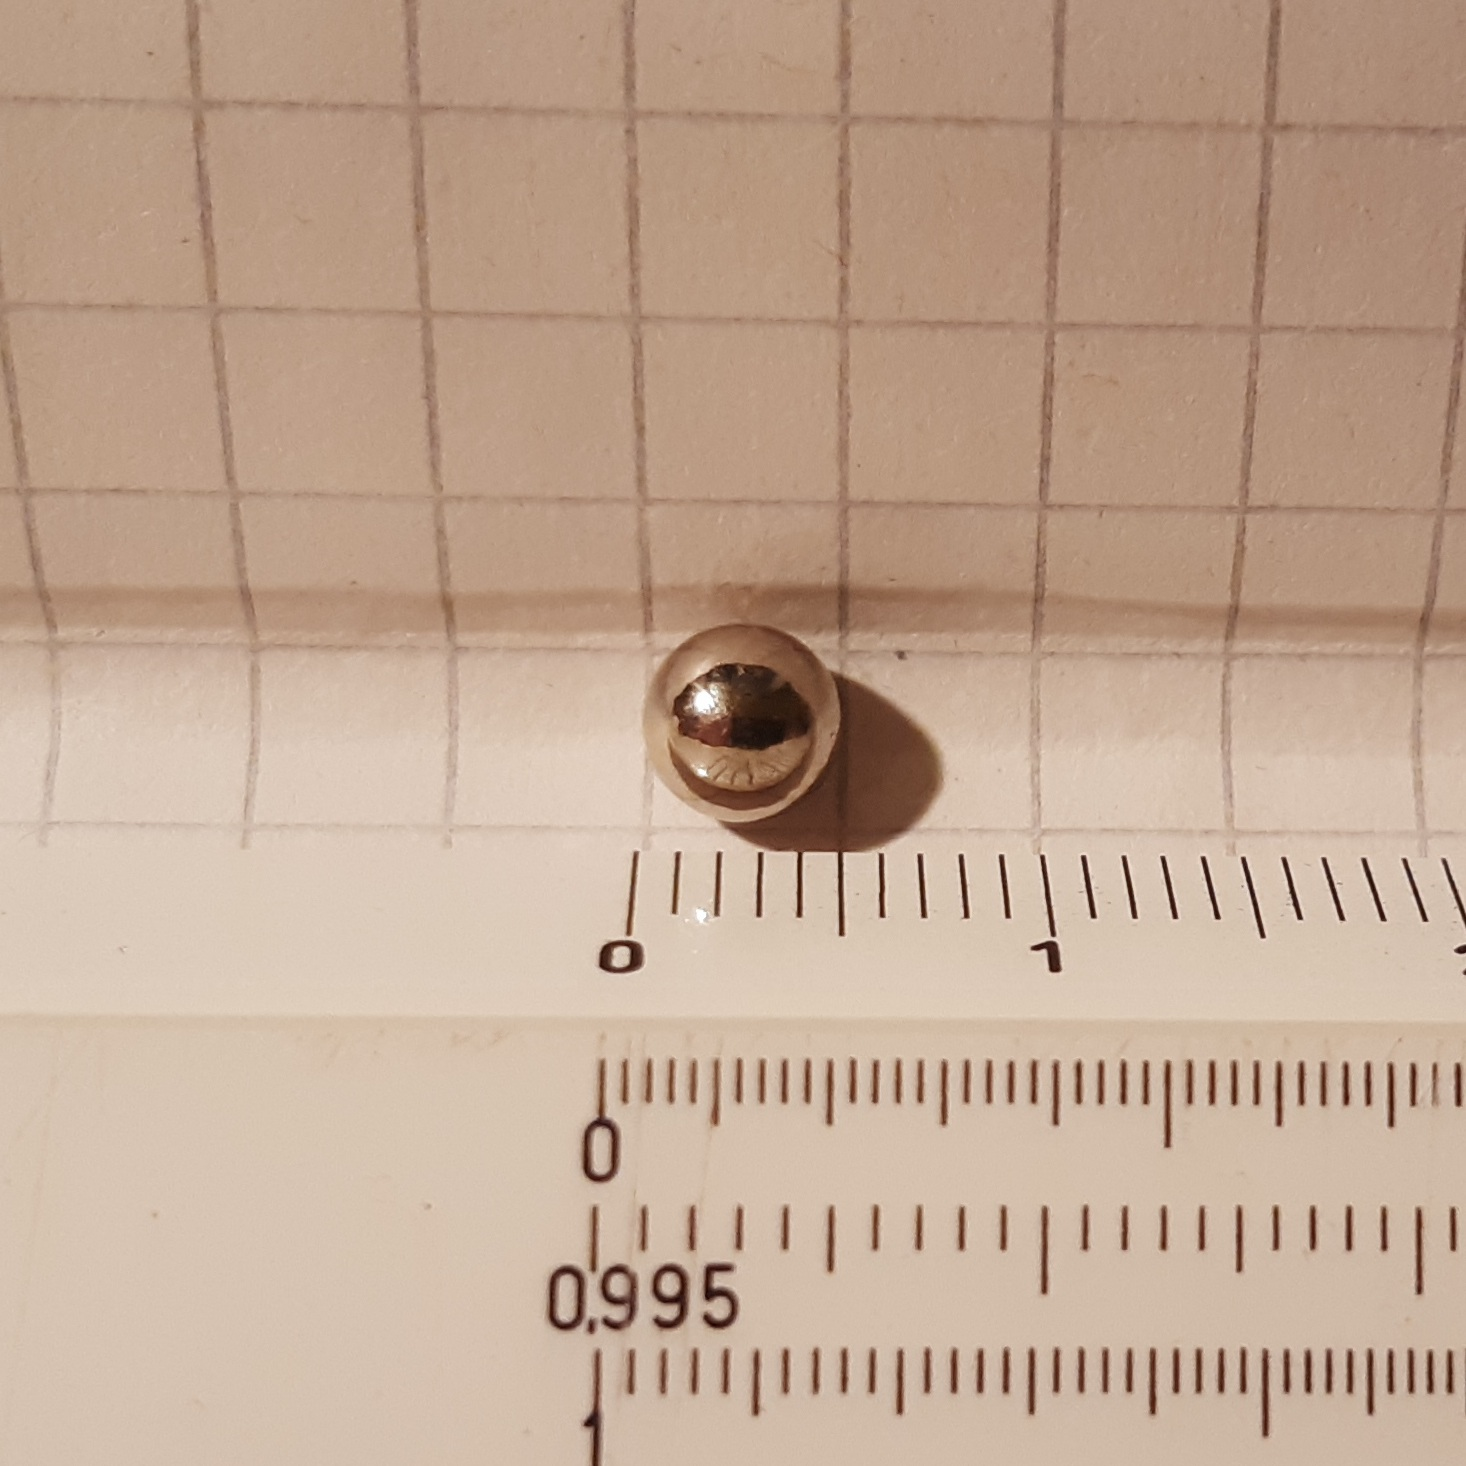
\includegraphics[width = \textwidth]{figures/koule5.jpg}
        \caption{$d = \SI{5}{\milli\metre}\text{, }m = \SI{0,45}{\gram}$}
    \end{subfigure}
    \hfill
    \begin{subfigure}[b]{.3\textwidth}
        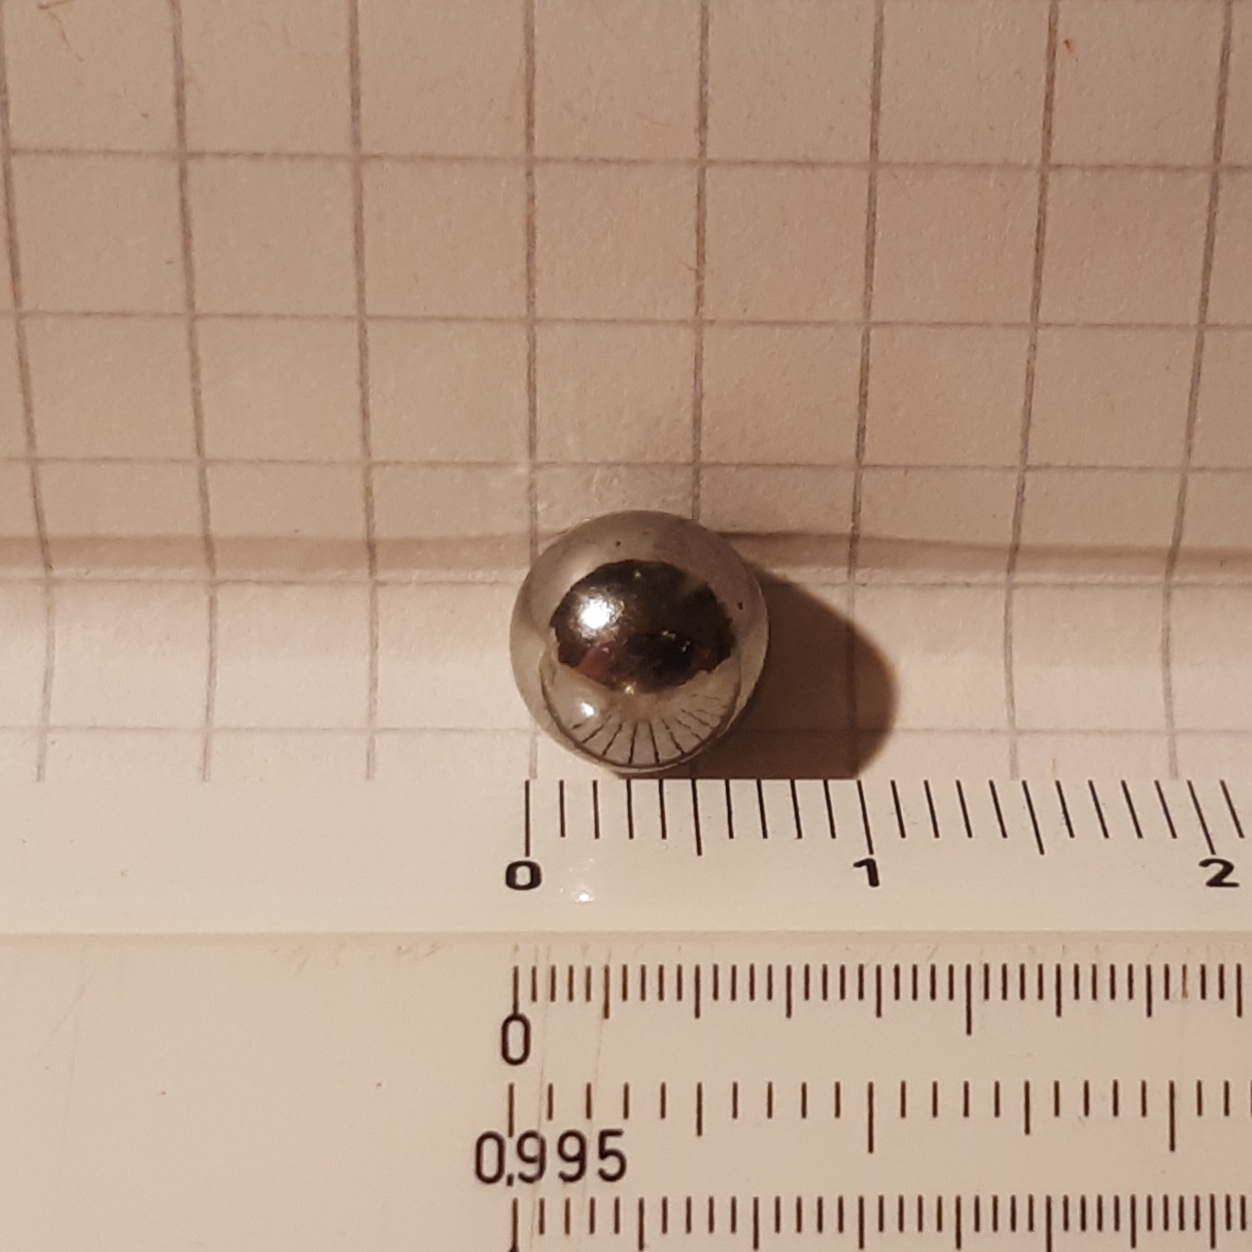
\includegraphics[width = \textwidth]{figures/koule8.jpg}
        \caption{$d = \SI{8}{\milli\metre}\text{, }m = \SI{2}{\gram}$}
    \end{subfigure}
    \hfill
    \begin{subfigure}[b]{.3\textwidth}
        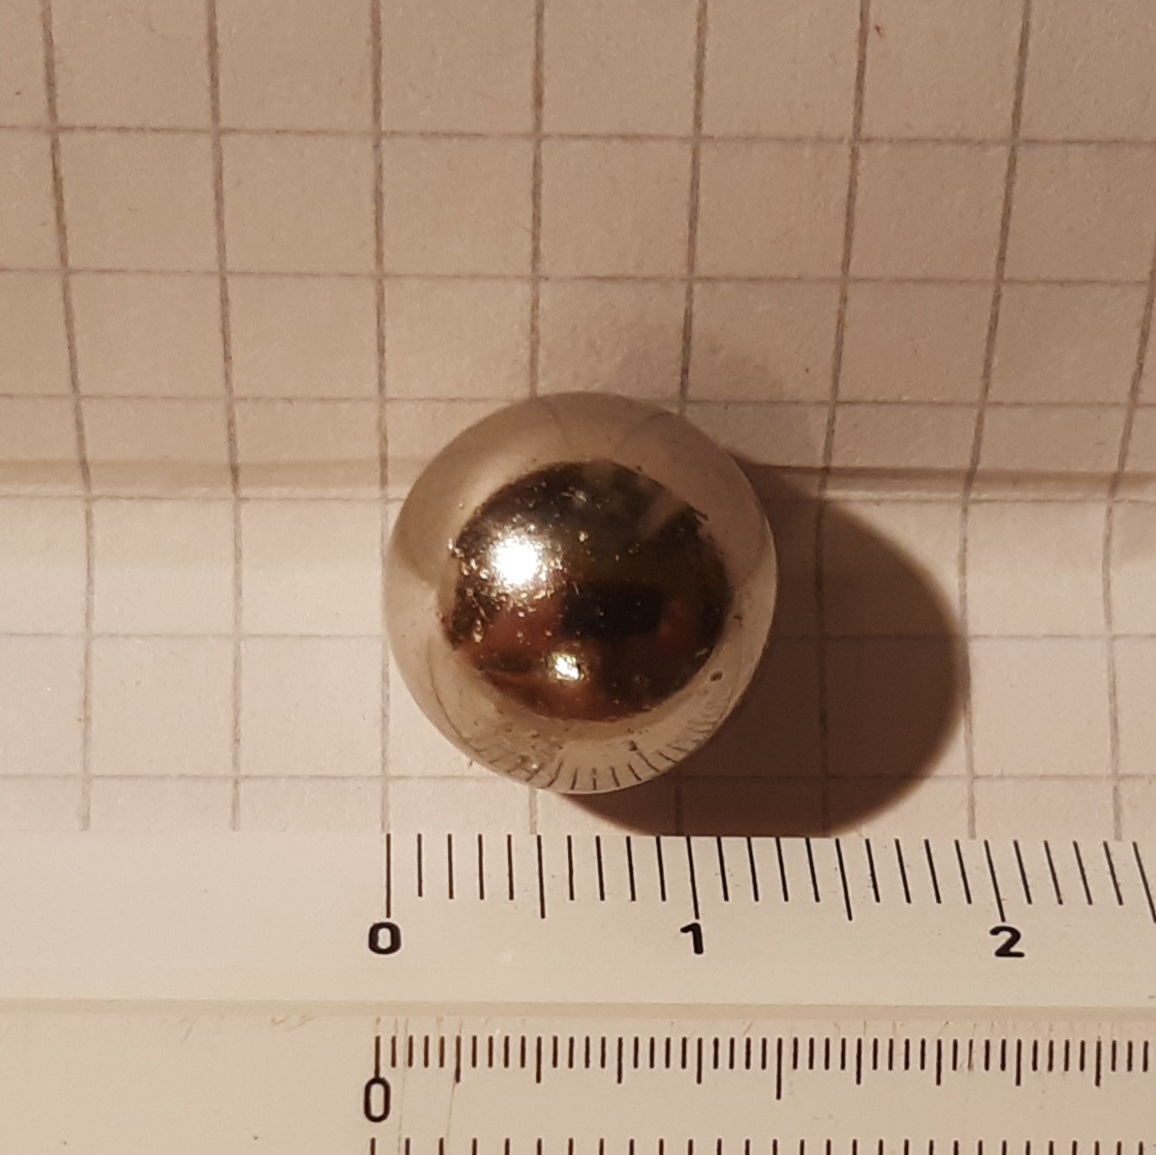
\includegraphics[width = \textwidth]{figures/koule13.jpg}
        \caption{$d = \SI{13}{\milli\metre}\text{, }m = \SI{8}{\gram}$}
    \end{subfigure}
    \caption{Neodymové magnety použité jako tělíska při testování tělískového viskozimetru. Údaje získané z~webových stránek \url{e-shop.magsy.cz}.}
    \label{fig:koule}
\end{figure}

%%%%%%%%%%%%%%%%%%%%%%%%%%%%%%%%%%%%%%%%%%%%%%%%%%%%%%%%%%%%%%%%%%%%%%
\subsection{Nálevkový viskozimetr}%%%%%%%%%%%%%%%%%%%%%%%%%%%%%%%%%%%%
%%%%%%%%%%%%%%%%%%%%%%%%%%%%%%%%%%%%%%%%%%%%%%%%%%%%%%%%%%%%%%%%%%%%%%

Pro výsledky předchozích zkoušek (příliš vysoká viskozita čokolády) byla možnost použití nálevkového viskozimetru zavržena bez rozsáhlejšího testování.

%%%%%%%%%%%%%%%%%%%%%%%%%%%%%%%%%%%%%%%%%%%%%%%%%%%%%%%%%%%%%%%%%%%%%%
\subsection{Rotační viskozimetr}%%%%%%%%%%%%%%%%%%%%%%%%%%%%%%%%%%%%%%
%%%%%%%%%%%%%%%%%%%%%%%%%%%%%%%%%%%%%%%%%%%%%%%%%%%%%%%%%%%%%%%%%%%%%%

Pro nevhodnost všech ostatních měřicích metod bylo rozhodnuto o~použití rotačního viskozimetru. Později byly za účelem ověření opakovatelnosti měření naměřeny dvě várky téže čokolády (Figaro) s~pozitivním výsledkem (viz data v~tabulce č.~\ref{tab:data_raw_dpas2} v~příloze).

%%%%%%%%%%%%%%%%%%%%%%%%%%%%%%%%%%%%%%%%%%%%%%%%%%%%%%%%%%%%%%%%%%%%%%
\newpage%%%%%%%%%%%%%%%%%%%%%%%%%%%%%%%%%%%%%%%%%%%%%%%%%%%%%%%%%%%%%%
\section{Aparatura}%%%%%%%%%%%%%%%%%%%%%%%%%%%%%%%%%%%%%%%%%%%%%%%%%%%
%%%%%%%%%%%%%%%%%%%%%%%%%%%%%%%%%%%%%%%%%%%%%%%%%%%%%%%%%%%%%%%%%%%%%%
%%%%%%%%%%%%%%%%%%%%%%%%%%%%%%%%%%%%%%%%%%%%%%%%%%%%%%%%%%%%%%%%%%%%%%

%%%%%%%%%%%%%%%%%%%%%%%%%%%%%%%%%%%%%%%%%%%%%%%%%%%%%%%%%%%%%%%%%%%%%%
\subsection{Použité pomůcky}%%%%%%%%%%%%%%%%%%%%%%%%%%%%%%%%%%%%%%%%%%
%%%%%%%%%%%%%%%%%%%%%%%%%%%%%%%%%%%%%%%%%%%%%%%%%%%%%%%%%%%%%%%%%%%%%%

Rotační viskozimetr, teploměr, hrnec nebo velká krystalizační miska, kádinka, rychlovarná konvice, laboratorní stojan, laboratorní zvedáček, držáky, křížové svorky, skleněná tyčinka či jiné vhodné míchadlo, hadice nebo skleněná trubička vhodného tvaru a~rozměrů, další nádoby, případně: termostat, laboratorní zdroj nebo jiný výkonný zdroj stejnosměrného napětí, baterie typu PP3 (\SI{9}{\volt}), měděný drát (nebo jiný s~vyšší rezistivitou), různé propojovací kabely a~dráty, elektrický budík, výkonové rezistory \SI{3,3}{\ohm} nebo jiné vhodnější.

%%%%%%%%%%%%%%%%%%%%%%%%%%%%%%%%%%%%%%%%%%%%%%%%%%%%%%%%%%%%%%%%%%%%%%
\subsection{Popis aparatury}%%%%%%%%%%%%%%%%%%%%%%%%%%%%%%%%%%%%%%%%%%
%%%%%%%%%%%%%%%%%%%%%%%%%%%%%%%%%%%%%%%%%%%%%%%%%%%%%%%%%%%%%%%%%%%%%%

Ústřední částí aparatury je vodní lázeň. Krystalizační miska naplněná vodou je umístěna na laboratorním zvedáčku. V~krystalizační misce je umístěna kovová kádinka (součástí příslušenství viskozimetru) určená k~tavení čokolády (standardně bylo taveno \SI{100}{\gram} čokolády). Teplota vody v~lázni je monitorována teploměrem. \label{sec:teploměr}
V~mém případě byl použit meteorologický teploměr půdní lomený (z~vlastní sbírky), jehož měřicí kapalinou je rtuť. Tento teploměr je vhodný díky svému tvaru, měřicímu rozsahu \SI{-21}{}~--~\SI{61}{\degreeCelsius}, přesností odečítání teploty na~\SI{0,1}{\degreeCelsius} a~krátké hysterezi. Fotografii teploměru je možné si prohlédnout na obr.~\ref{fig:teploměr} v~příloze. Do kádinky s~čokoládou je ponořeno měřicí vřeteno viskozimetru. Čokoláda může být pro zajištění teplotní homogenity míchána skleněnou tyčinkou nebo jiným vhodným míchadlem. Celá aparatura je upevněna na laboratorním stojanu.
\par\noindent
Teplota lázně je udržována přiléváním vroucí vody z~rychlovarné konvice do lázně při poklesu teploty pod žádanou mez. Jedná se tak o~práci vyžadující značnou pozornost a~časté monitorování teploty obsluhou aparatury. Navíc je teplota lázně měněna skokově a~rozsah, ve kterém se teplota lázně pohybuje, je velký (\SI{\pm 1,5}{\degreeCelsius} při teplotách kolem \SI{40}{\degreeCelsius}, \SI{\pm 4}{\degreeCelsius} při teplotách kolem \SI{60}{\degreeCelsius}). Množství vody v~lázni se zároveň neustále zvyšuje a~vodu je proto nutné při naplnění misky odčerpat do jiné nádoby hadičkou nebo trubičkou, která je v~lázni ponořena.
\par
\label{Vřetena}
\noindent
K~měření viskozity byl použit rotační viskozimetr značky Haake model Viscotester VT-02. Konstrukcí se jedná o~viskozimetr dle Brookfielda. Použité měřicí vřeteno bylo voleno podle viskozity čokolády. Technické údaje o~vřetenech tohoto viskozimetru jsou k~nalezení v~tabulce \ref{tab:vretena}. Pro čokolády s~vyšší viskozitou bylo použito vřeteno ve tvaru nízkého válce pro rozsah \SI{100}{}~--~\SI{4000}{\deci\pascal\second}, (v~tabulce označováno jako vřeteno č.~2). Pro čokolády s~nižší viskozitou bylo použito vřeteno ve tvaru vysokého válce pro měřicí rozsah \SI{3}{}~--~\SI{160}{\deci\pascal\second}, (v~tabulce hodnot označováno jako vřeteno č.~1).~\cite{man:VT-02}

\begin{figure}[ht]
    \begin{minipage}[b]{0.3\linewidth}
        \centering
        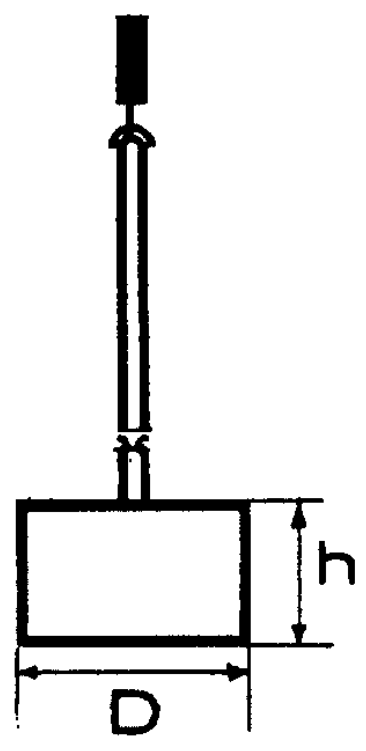
\includegraphics[width=0.5\textwidth]{figures/vreteno.png}
        \caption{Obecný nákres rotačního vřetena.~\cite{man:VT-02}}
        \label{fig:vreteno}
    \end{minipage}
    \hspace{0.5cm}
    \begin{minipage}[b]{0.65\linewidth}
        \begin{table}[H]
            \centering
            \begin{tabular}{|c|c|c|c|}
                \hline
                Číslo & Měřicí rozsah [\SI{}{\deci\pascal\second}] & D [\SI{}{\milli\metre}] & h [\SI{}{\milli\metre}] \\ \hline
                $1$ & $3 - 150$ & $24,0\pm 0,1$ & $53,0\pm0,1$ \\ \hline
                $2$ & $100 - 4000$ & $15,0\pm 0,05$ & $1^{+0,05}_{-0}$ \\ \hline
                $3$ & $0,3 - 13$ & $45,1^{+0}_{-0,3}$ & $47,0^{+0,2}_{-0}$ \\ \hline
            \end{tabular}
            \caption{Rozměry a~měřicí rozsahy vřeten dodávaných k~viskozimetru Haake Viscotester VT-02. Hodnoty $D$ a~$h$ srovnejte s~obrázkem~\ref{fig:vreteno}.~\cite{man:VT-02}}
            \label{tab:vretena}
        \end{table}
        \label{fig:figure2}
    \end{minipage}
\end{figure}

\par\noindent
První implementace aparatury je vyfocena na obrázku~\ref{fig:aparatura}, zbytek fotografií aparatury je k~nalezení v~příloze.

\begin{figure}
    \begin{subfigure}[b]{.5\textwidth}
        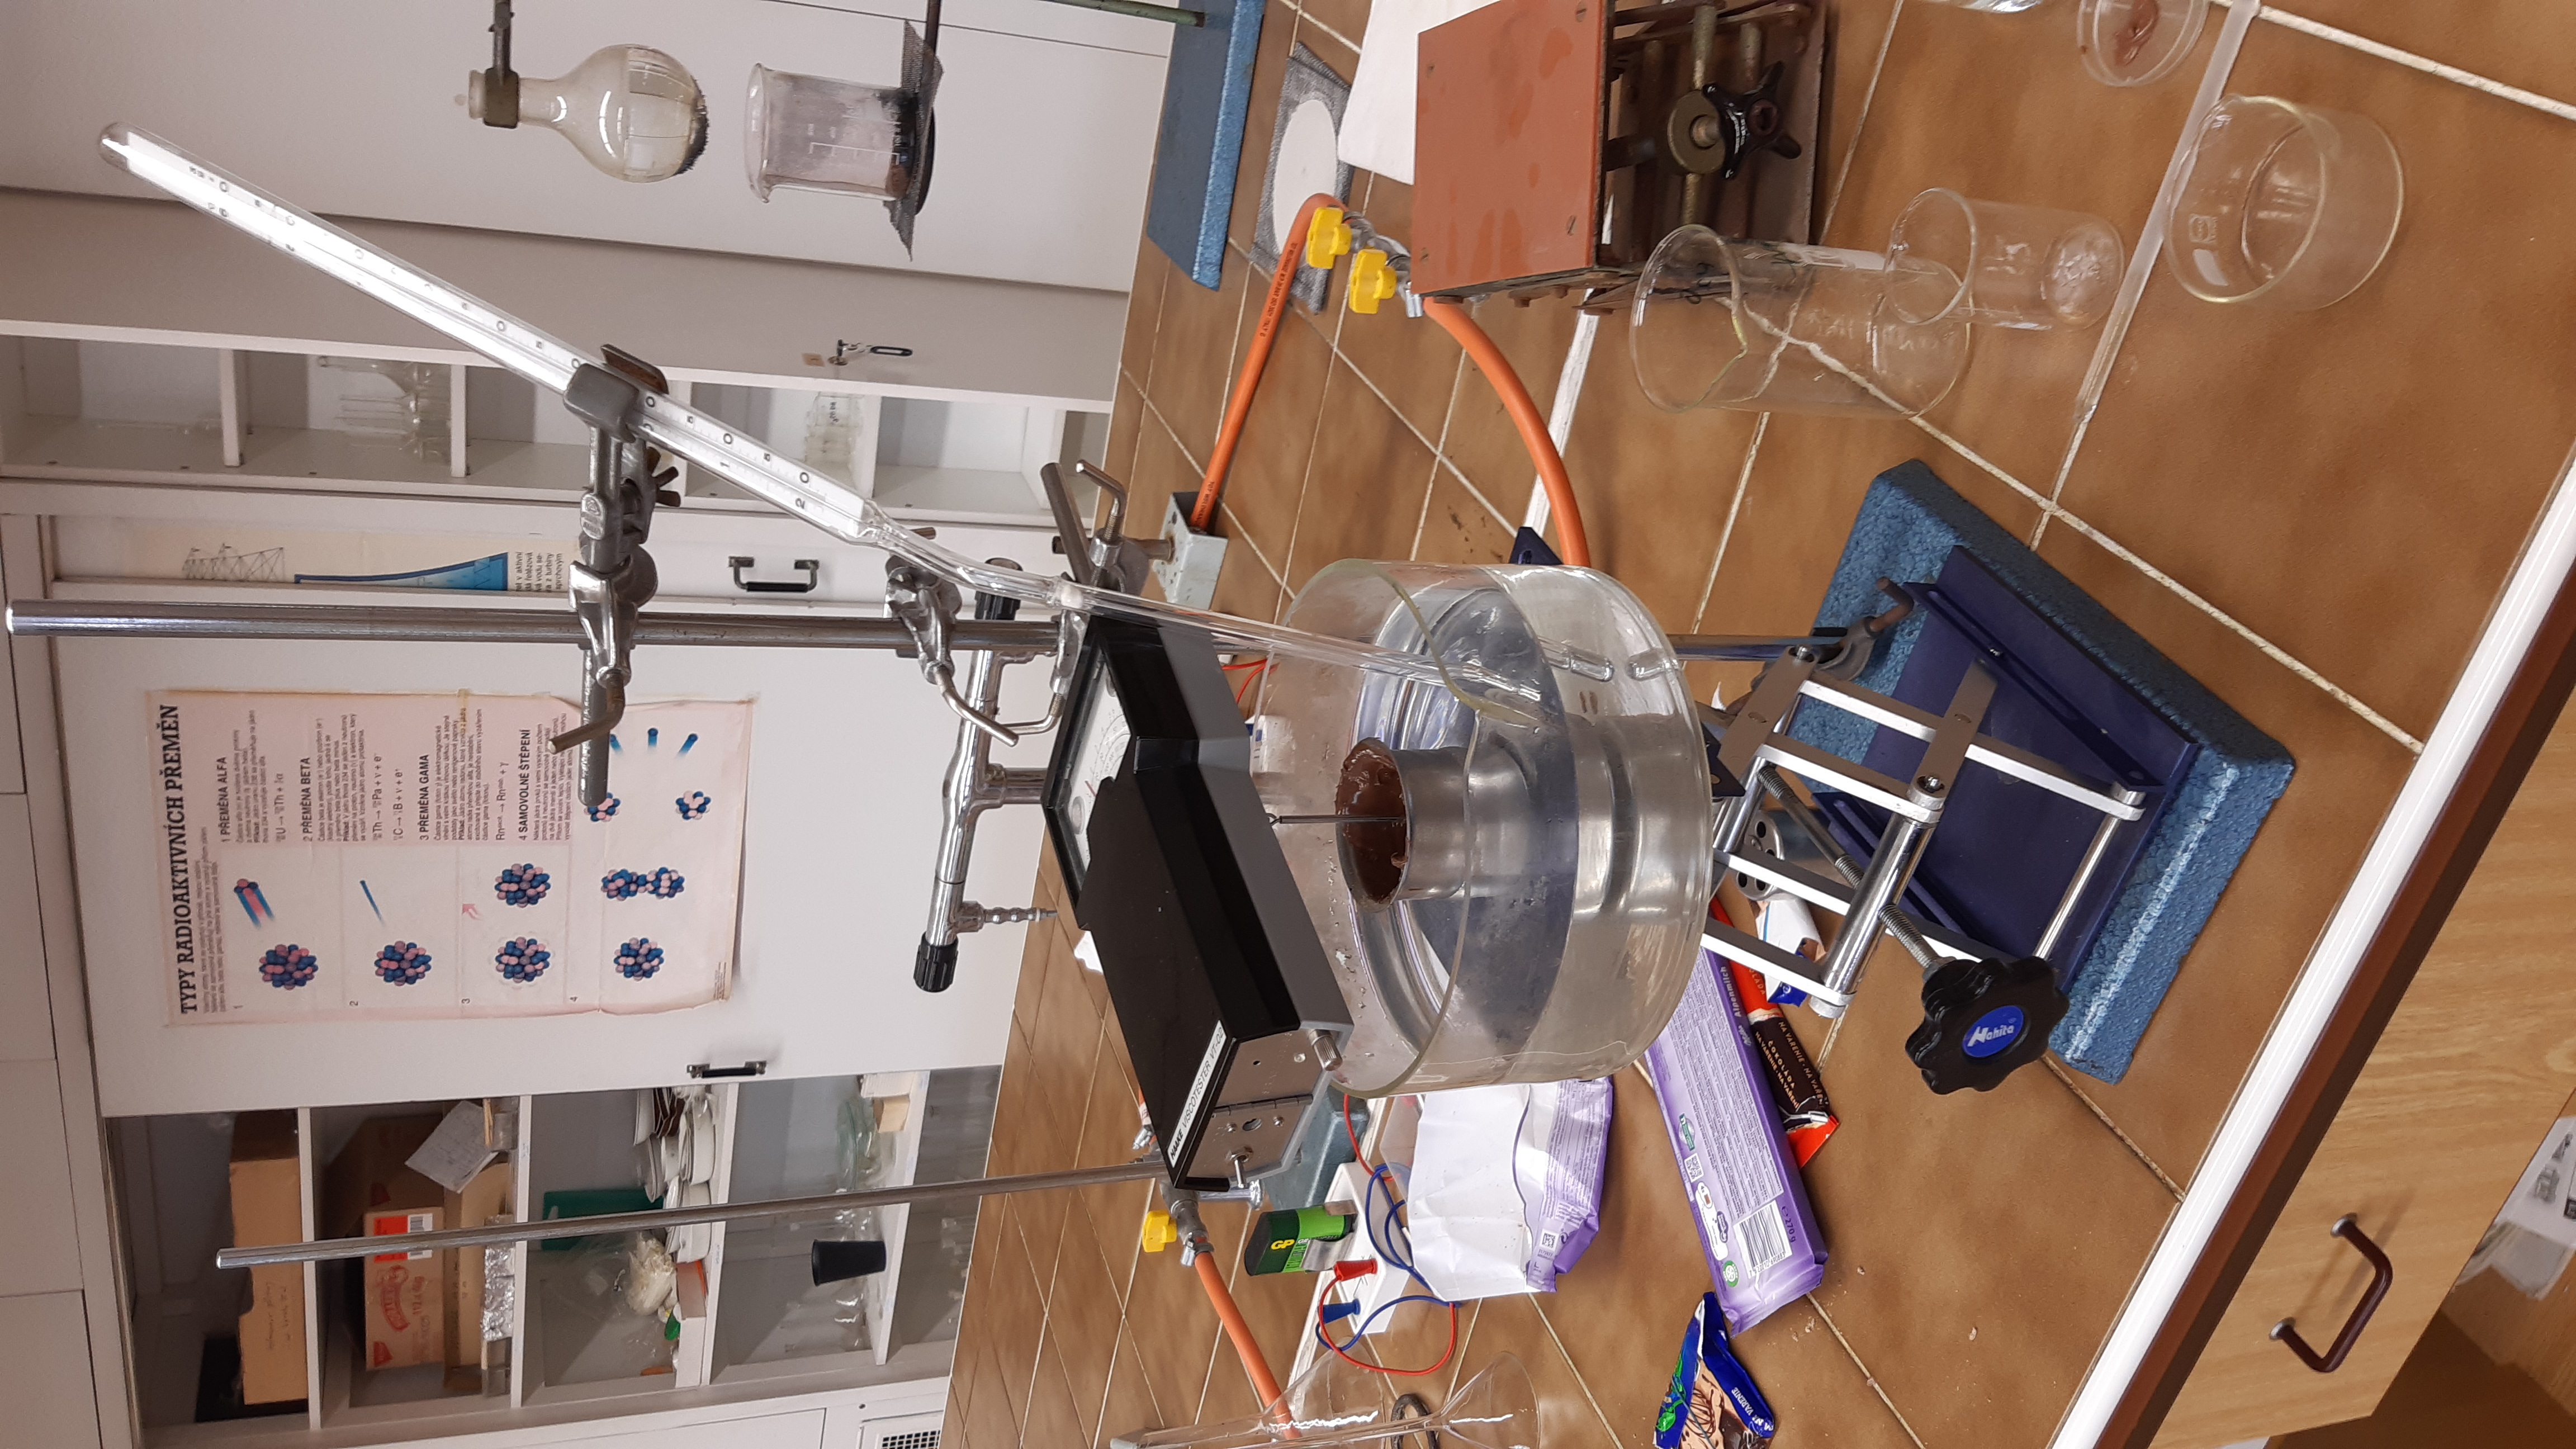
\includegraphics[angle = 270, width = \textwidth]{figures/aparatura_1.jpg}
    \end{subfigure}
    \hfill
    \begin{subfigure}[b]{.5\textwidth}
        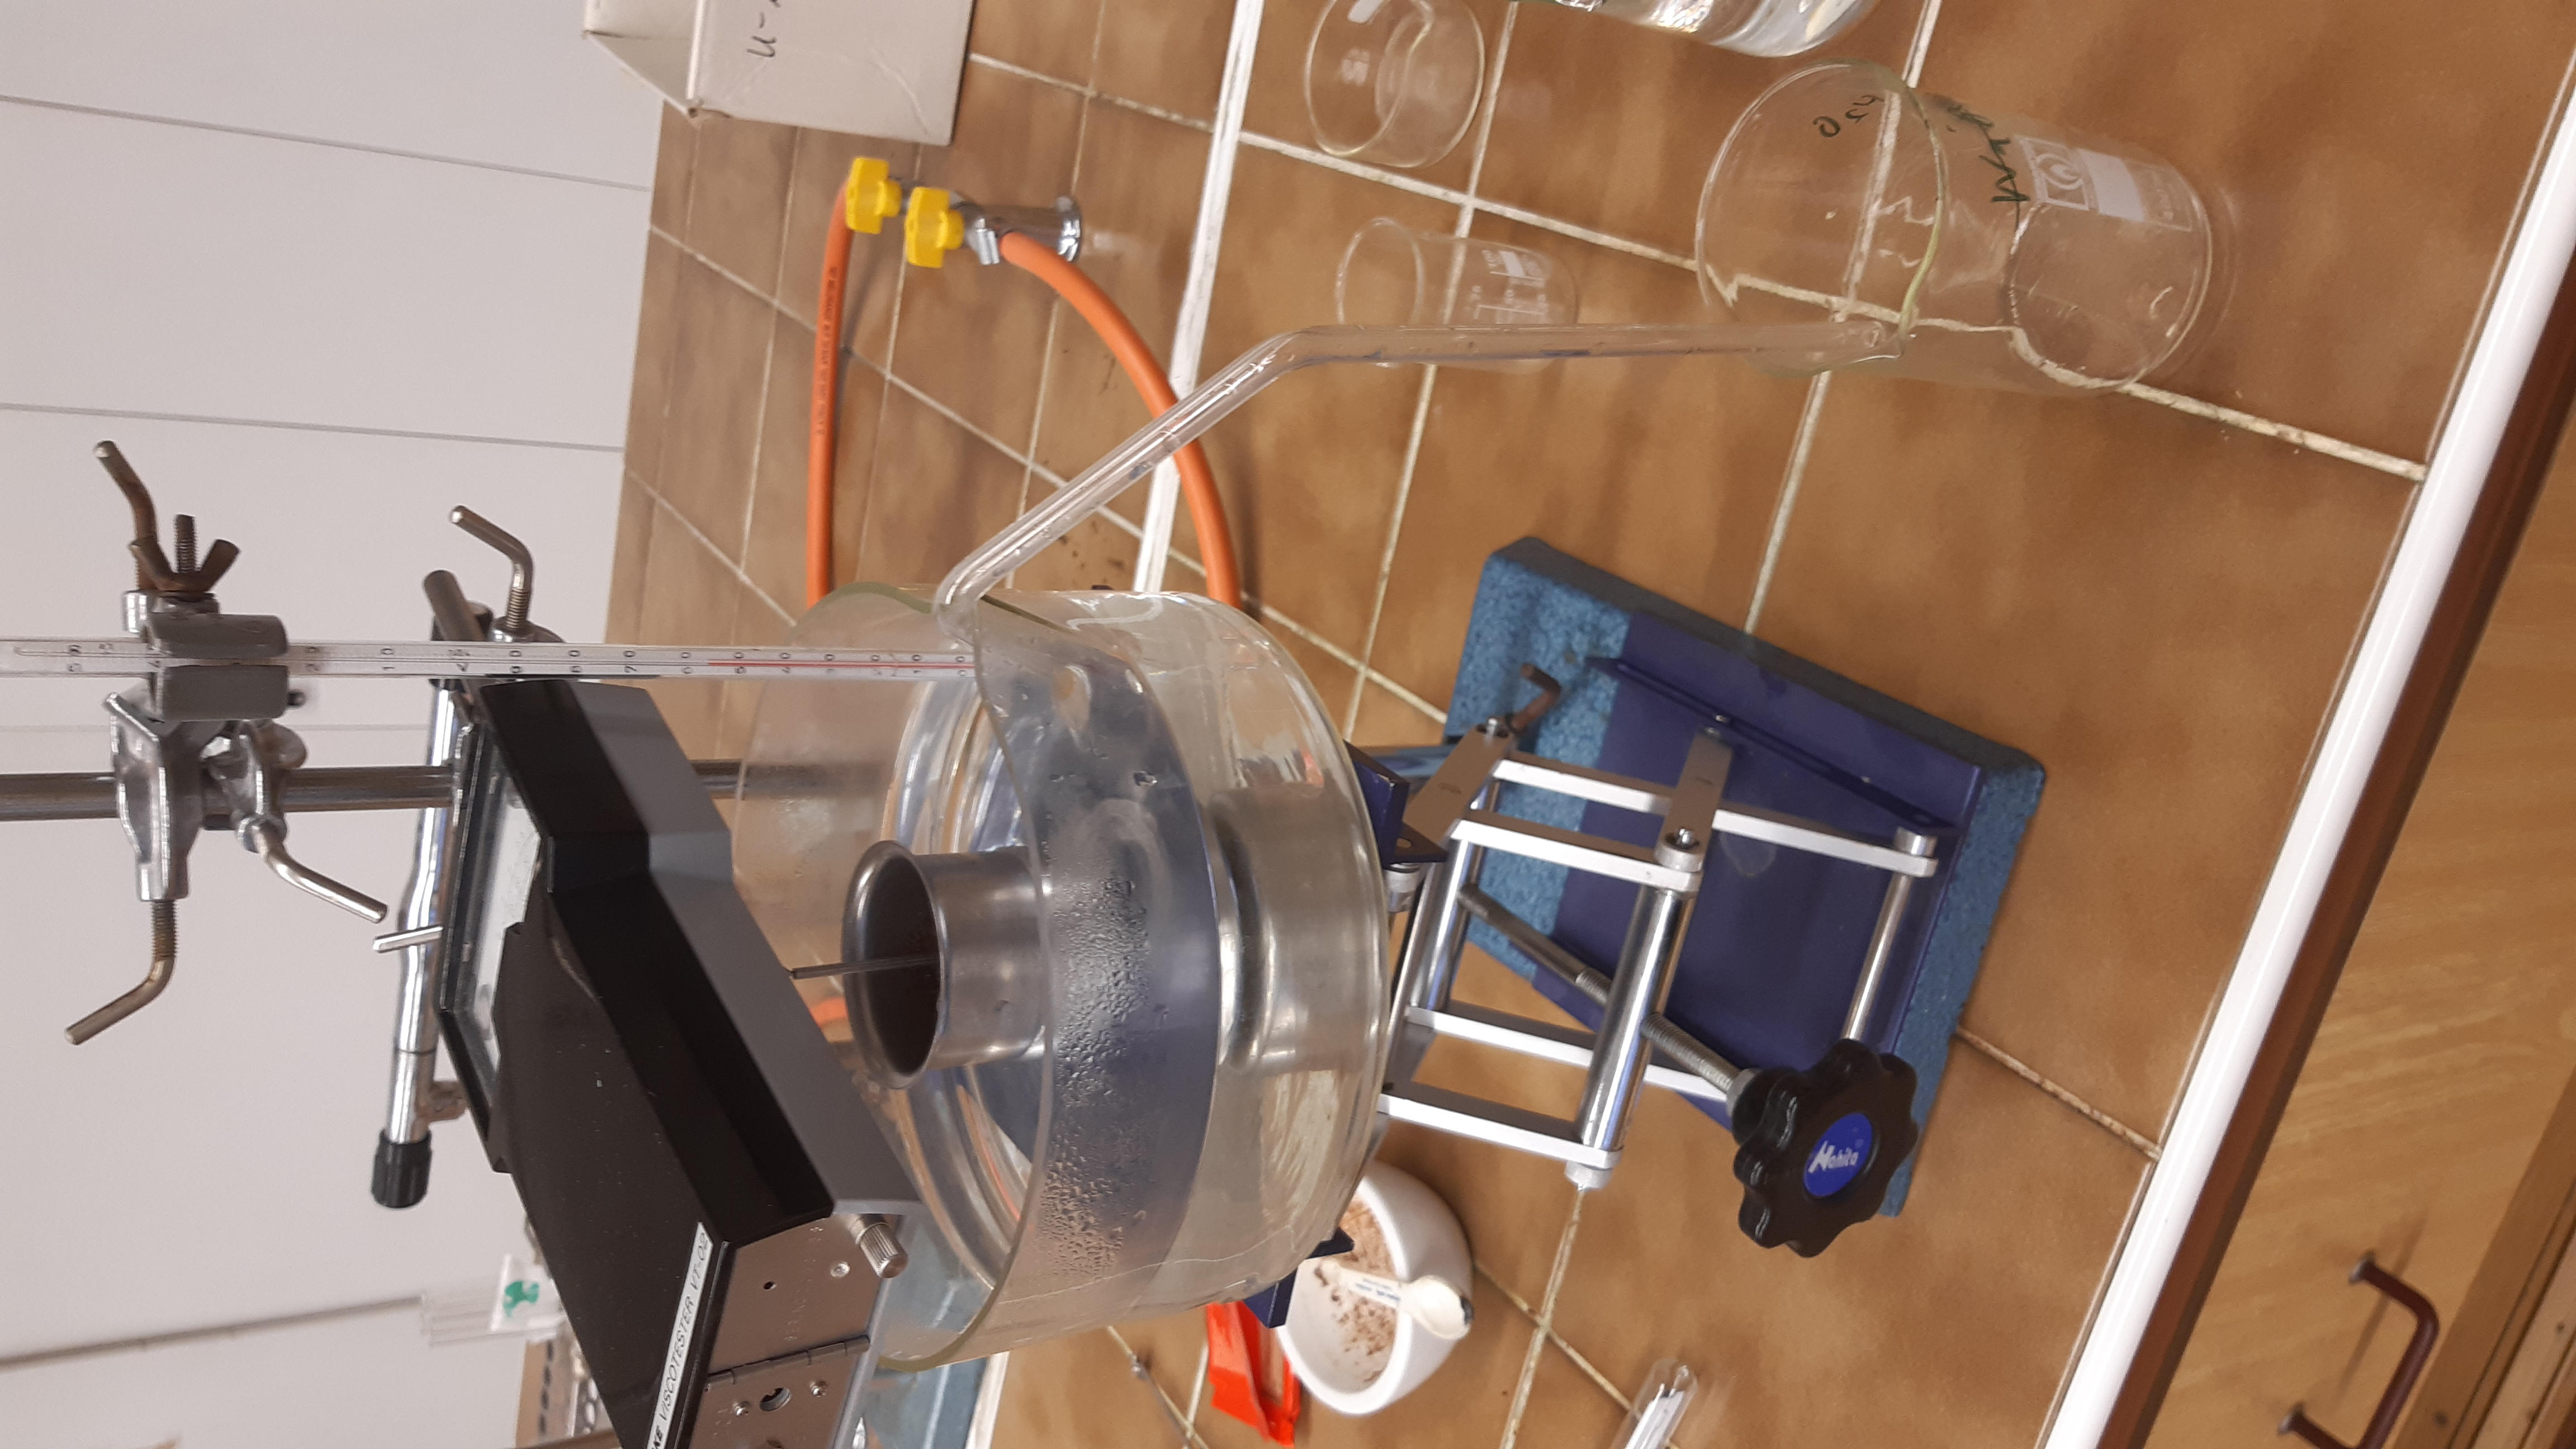
\includegraphics[angle = 270, width = \textwidth]{figures/aparatura_2.jpg}
    \end{subfigure}
    \caption{První implementace aparatury. Velká krystalizační miska na zvedáčku tvoří vodní lázeň. V~ní je umístěna kovová kádinka s~čokoládovou taveninou. Do ní je vloženo měřicí vřeteno rotačního viskozimetru. Teplota lázně je měřena teploměrem: vlevo je použit přesný meteorologický teploměr (specifikace viz str.~\pageref{sec:teploměr}), vpravo je použit jiný, neznámý laboratorní teploměr, který byl schopen měřit vyšší teploty. Teplota lázně byla regulována přiléváním horké vody do lázně. Na pravém obrázku je pak vidět skleněná trubička, kterou byla přebytečná voda z~lázně odčerpávána.}
    \label{fig:aparatura}
\end{figure}

\par\noindent
V~domácím prostředí byla aparatura za účelem usnadnění měření a~snížení nároků na pozornost obsluhy modifikována. Do vodní lázně bylo umístěno topné těleso spínané termostatem, který je na obrázku~\ref{fig:termostat}. Termostat umožňuje měřit teploty od \SI{-50} do \SI{110}{\degreeCelsius} s~udávanou přesností na \SI{0,1}{\degreeCelsius}. Teplotní čidlo termostatu tvoří termistor se záporným teplotním koeficientem ve vodotěsném pouzdře. Samotný termostat požaduje napájecí napětí \SI{12}{\volt}, v~této aparatuře byla k~jeho pohonu použita \SI{9}{\volt} baterie (PP3). Jako topné těleso byl použit smotaný měděný drát o~odporu zhruba \SI{5}{\ohm}. Topné těleso bylo napájené laboratorním zdrojem, který je schopen dodávat maximální proud \SI{5}{\ampere}. Použitím vztahu $P=RI^2$ vyplývá, že použité topné těleso mělo příkon kolem \SI{125}{\watt}. Teplota lázně byla i~nadále kontrolována rtuťovým teploměrem. Takto upravenou aparaturu lze, alespoň v~teoretickém případě, nastavit na požadovanou teplotu, počkat na zahřátí lázně a~čokolády, následně provést měření, termostat přenastavit na vyšší teplotu a~opakovat. Tato modifikace by tedy v~ideálním případě práci ušetřila. Termostat byl navíc schopen udržovat teplotu v~rozsahu \SI{\pm 0,5}{\degreeCelsius} kolem požadované teploty (podstatně užší rozsah oproti manuální alternativě).

\begin{figure}
    \centering
    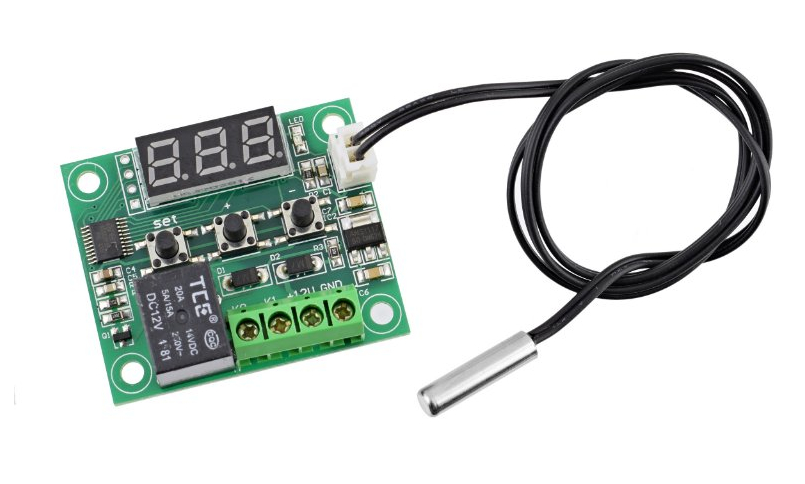
\includegraphics[width = 0.5\linewidth]{figures/termostat.jpg}
    \caption{Použitý termostat.~\cite{Figure:termostat}}
    \label{fig:termostat}
\end{figure}

%%%%%%%%%%%%%%%%%%%%%%%%%%%%%%%%%%%%%%%%%%%%%%%%%%%%%%%%%%%%%%%%%%%%%%
\subsection{Problémy aparatury}%%%%%%%%%%%%%%%%%%%%%%%%%%%%%%%%%%%%%%%
%%%%%%%%%%%%%%%%%%%%%%%%%%%%%%%%%%%%%%%%%%%%%%%%%%%%%%%%%%%%%%%%%%%%%%

Výše popsaná implementace spínaného topného tělesa však skýtala několik problémů:
\begin{enumerate}[noitemsep, topsep = 0pt]
    \item \underline{Problém}: Elekromagnet, který spíná relé termostatu, \SI{9}{\volt} baterii po několika desítkách minut vybil natolik, že termostat sice pracoval, ale baterie nebyla schopná dodat dostatečný proud k~sepnutí kontaktů a~zapnutí topného tělesa. Aparatura tedy z~dálky vypadala jako správně fungující, nebyla však schopná vyhřívání a~tedy udržení teploty.
    \par \underline{Řešení}: Jako nejjednodušší, nikoliv však trvalé řešení, se ukázalo vyměnit baterii za novou. Několik vybitých baterií šlo též zapojit paralelně a~tím zvýšit dodávaný proud. Obě tato řešení však fungovala velice dočasně. Nakonec bylo rozhodnuto pro napájení termostatu stejnosměrným \SI{13}{\volt} zdrojem z~elektrické sítě, čímž byl problém odstraněn trvale.
    \item \underline{Problém}: Kontakty spojovacích kabelů, které byly k~topnému tělesu připojeny, byly rozkládány elektrolýzou a~docházelo tedy k~přerušení obvodu.
    \par \underline{Řešení}: Konce spojovacích kabelů byly vyjmuty z~vodní lázně a~nahrazeny novými, nepoškozenými. V~pozdější verzi aparatury byla lázeň plněna destilovanou vodou, čímž došlo k~odstranění tohoto problému.
    \item \underline{Problém}: Topné těleso po pár hodinách přestává vést elektrický proud. Po zhruba dvou hodinách odpor topného tělesa náhle skokově vzrostl na jednotky až desítky \SI{}{\kilo\ohm}. Toto je nejspíše způsobeno degradací materiálu. Tenká smaltovaná izolace měděného drátu byla narušena v~místech, kde byl drát ohnutý. Tato narušení se mohla zesilovat opětovným ohýbáním drátu tam a~zpět (při opětovném uzavírání a~otevírání obvodu se elektromagnetická síla projevovala značným cukáním topného drátu tam a~zpět, což mohlo po několika hodinách a~tedy stovkách cyklů materiál unavit). V~těchto bodech byl materiál zároveň vystaven vodě v~lázni a~tedy i~působení elektrolýzy. Příčina zvýšení odporu drátu však stále zůstává neznámá.
    \par \underline{Řešení}: Měděný drát topného tělesa byl po každém selhání nahrazen novým.
    \item \underline{Problém}: Horké kontakty topného tělesa na vzduchu oxidovaly a~docházelo tak k~rozpojení obvodu.
    \par \underline{Řešení}: Vrstva oxidu byla v~pravidelných intervalech odstraňována pomocí nože nebo smirkového papíru, případně bylo celé topné těleso nahrazeno novým.
    \item \underline{Problém}: Termostat při teplotách nad \SI{57}{\degreeCelsius} ukazuje nesmyslné hodnoty, spíná tedy nesprávně a~není schopen udržet teplotu ve stanoveném rozsahu. Jedná se nejspíše o~vadu termostatu.
    \par \underline{Řešení}: Tuto závadu se nepodařilo odstranit, při teplotách nad \SI{57}{\degreeCelsius} byla tedy teplota monitorována a~upravována manuálně. Posléze bylo od měření při teplotách vyšších než \SI{55}{\degreeCelsius} úplně upuštěno.
    \item \underline{Problém}: Voda se z~vodní lázně postupně odpařuje (platí pouze u~konstrukce aparatury s~topným tělesem).
    \par \underline{Řešení}: Voda byla do lázně v~případě nutnosti dolévána. Byla tím však narušována udržovaná teplota lázně.
    \item \underline{Problém}: Teplota lázně naměřená termostatem se liší od teploty naměřené rtuťovým teploměrem.
    \par \underline{Řešení}: Při měření byla zaznamenána velikost chyby termostatu \SI{1}{\degreeCelsius}. O~tuto chybu pak byly výsledky měření posunuty (rtuťový teploměr byl považován za přesnější).
\end{enumerate}
Po několikáté výměně topného tělesa (v~důsledku problémů 3 a~4) v~mé osobní zásobě došel měděný drát, od aparatury v~této sestavě tedy bylo nutné upustit. Aparatura byla znovu modifikována: namísto topného tělesa byl do okruhu zapojen elektrický budík, napájen z~laboratorního zdroje napětím \SI{1,5}{\volt}. Ten obsluhu aparatury upozorňoval zvukovou signalizací pokaždé, když teplota lázně klesla pod stanovenou mez. Teplota lázně však musela být (pro absenci topného tělesa) udržována manuálně (varnou konvicí). I~tato implementace měla své limity (ukázalo se, že budík není stoprocentně funkční), jednalo se vskutku pouze o~provizorní řešení.
\par
Posléze byla aparatura opět modifikována a~jako topného tělesa bylo namísto měděného drátu použito soustavy výkonových \SI{3,3}{\ohm} rezistorů. Schema zapojení rezistorů je na obrázku \ref{fig:schema_zapojeni_rezistory}. Tím došlo k~odstranění problémů č.~3 a~4. Nebylo tak nutné spotřebovávat desítky metrů měděného drátu, jelikož prostředí lázně rezistory díky jejich obalu nepoškozovalo. 

\begin{figure}
    \centering
    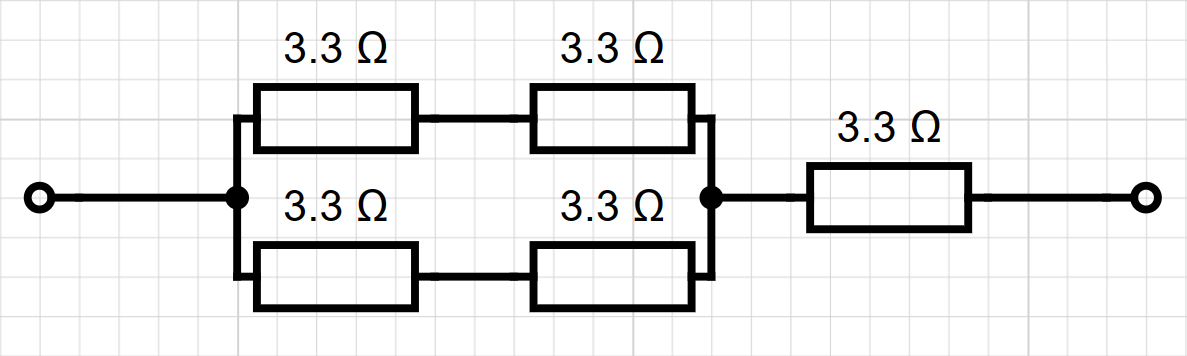
\includegraphics[width = 0.75\linewidth]{figures/rezistory.png}
    \caption{Schéma zapojení rezistorů, které byly použity jako topné těleso. Vytvořeno s~pomocí webové aplikace \url{www.circuit-diagram.org}.}
    \label{fig:schema_zapojeni_rezistory}
\end{figure}

\begin{figure}[h!]
    \begin{subfigure}[b]{.5\textwidth}
        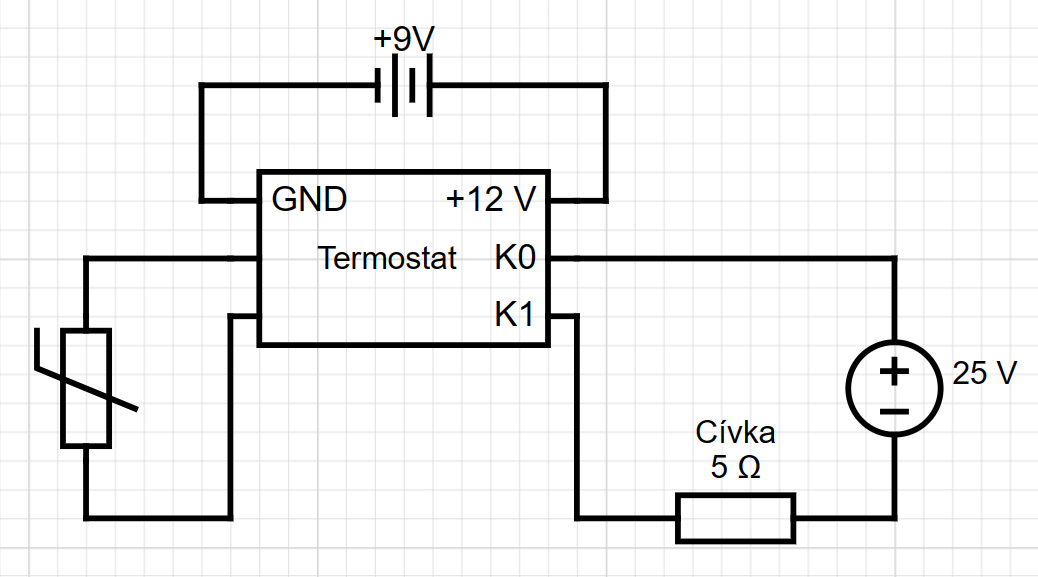
\includegraphics[width = \textwidth]{figures/zapojeni_1.png}
        \caption{První zapojení aparatury.}
    \end{subfigure}
    \hfill
    \begin{subfigure}[b]{.5\textwidth}
        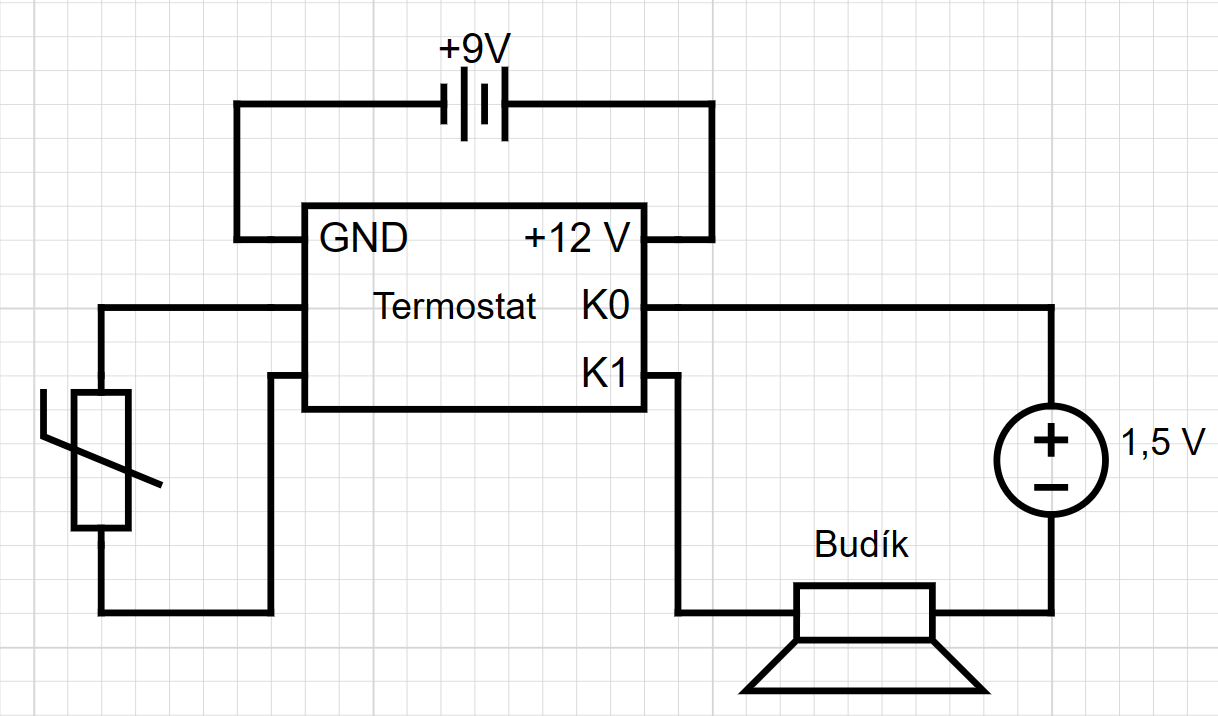
\includegraphics[width = \textwidth]{figures/zapojeni_2.png}
        \caption{Provizorní zapojení aparatury s~budíkem jakožto zvukovou signalizací.}
    \end{subfigure}
    \caption{Vyzkoušená zapojení aparatury. Vytvořeno s~pomocí webové aplikace \url{www.circuit-diagram.org}.}
    \label{fig:zapojeni_prvni}
\end{figure}

\begin{figure}[h!]
    \centering
    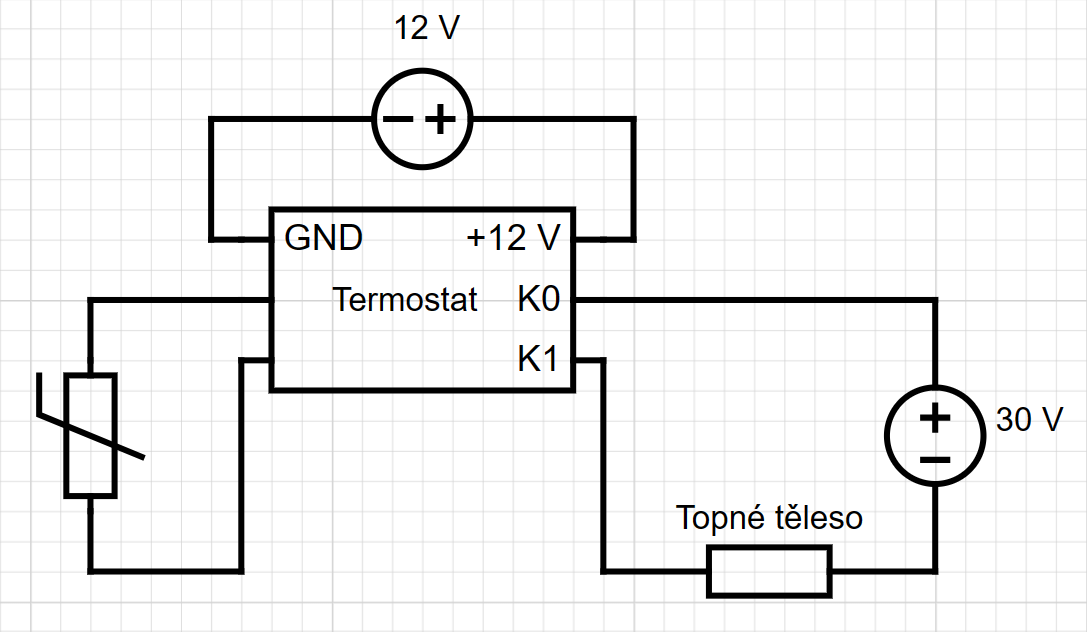
\includegraphics[width = 0.5\linewidth]{figures/zapojeni_3.png}
    \caption{Finální zapojení aparatury. Topné těleso je rozkreslené na obr.~\ref{fig:schema_zapojeni_rezistory}. Vytvořeno s~pomocí webové aplikace \url{www.circuit-diagram.org}.}
    \label{fig:zapojeni_final}
\end{figure}

Toto zapojení bylo vybráno z~důvodu, že ztrátový výkon použitých rezistorů byl pouze \SI{20}{\watt}. Napětí a~proud protékající celým topným tělesem byly \SI{30}{\volt} a~přibližně \SI{4}{\ampere}, topné těleso tedy mělo příkon zhruba \SI{120}{\watt}. Při rozložení tohoto příkonu zjistíme, že každý z~rezistorů v~levé části obr.~\ref{fig:schema_zapojeni_rezistory} má příkon \SI{15}{\watt}, což splňuje jeho provozní požadavky. Rezistor úplně vpravo má zde příkon \SI{60}{\watt}, což značně převyšuje jeho ztrátový výkon. I~přesto bylo k~tomuto zapojení přistoupeno, a~to z~důvodu, že bylo pořízeno pouze 10 těchto rezistorů. Pokud bychom chtěli zapojit do topného tělesa rezistorů 8, zbyly by pouze dva náhradní, což jsem považoval za riskantní. Naopak se nabízelo zapojení pouhých dvou rezistorů sériově, oba by pak měly příkon \SI{60}{\watt}, za to by však bylo hodně náhradních rezistorů pro případ, že by se některý z~použitých pro překročení ztrátového výkonu přepálil. Raději však bylo zvoleno zapojení na obrázku \ref{fig:schema_zapojeni_rezistory}, protože nabízí střední cestu mezi oběma alternativními zapojeními, topné těleso má větší povrch a~lépe a~rovnoměrněji tím pádem prohřívá lázeň a~v~případě poškození je možné sestavit ještě jedno úplně nové topné těleso. Riziko přepálení rezistoru jsem považoval za malé, jelikož byl rezistor chlazen právě vodní lázní, ve které byl umístěn. Skutečný ztrátový výkon rezistoru byl tedy o~mnoho vyšší, než oněch \SI{20}{\watt} udávaných na vzduchu.
\par\noindent
Schémata celkových zapojení aparatury v~různých provedeních jsou na obrázcích~\ref{fig:zapojeni_prvni} a~\ref{fig:zapojeni_final}.

%%%%%%%%%%%%%%%%%%%%%%%%%%%%%%%%%%%%%%%%%%%%%%%%%%%%%%%%%%%%%%%%%%%%%%
\newpage%%%%%%%%%%%%%%%%%%%%%%%%%%%%%%%%%%%%%%%%%%%%%%%%%%%%%%%%%%%%%%
\section{Průběh měření}%%%%%%%%%%%%%%%%%%%%%%%%%%%%%%%%%%%%%%%%%%%%%%%
%%%%%%%%%%%%%%%%%%%%%%%%%%%%%%%%%%%%%%%%%%%%%%%%%%%%%%%%%%%%%%%%%%%%%%
%%%%%%%%%%%%%%%%%%%%%%%%%%%%%%%%%%%%%%%%%%%%%%%%%%%%%%%%%%%%%%%%%%%%%%

\underline{\smash{Pomůcky}}: Výše popsaná aparatura, třecí miska s~tloučkem (nebo jiné náčiní vhodné k~drcení čokolády). 
\par \underline{Průběh}: Vodní lázeň byla předehřátá na \SI{37}{\degreeCelsius}. Do misky s~tloučkem bylo vloženo \SI{100}{\gram} čokolády, která byla následně nadrcena. Většinou nebylo nutné čokoládu vážit -- \SI{100}{\gram} je standardní hmotnost jednoho balení. Malé množství drcené čokolády (okolo jedné čajové lžičky) bylo nasypáno do kovové kádinky, která byla vložena do lázně. Po částečném roztavení čokolády v~kádince byla postupně přisypávána další čokoládová drť. Čokoládová tavenina byla po celou dobu míchána vhodným míchadlem. Po vložení celého vzorku do kádinky byla tavenina ponechána při teplotě \SI{37}{\degreeCelsius} ještě několik desítek minut a~soustavně míchána, aby byla zajištěna teplotní homogenita a~úplné roztavení čokolády, včetně rozbití vzniklých hrudek.
\par
Do této homogenní čokoládové taveniny bylo ponořeno měřicí vřeteno viskozimetru tak, aby jeho spodní část zůstala zhruba \SI{5}{\milli\metre} nad dnem kádinky. Samotné měření pak probíhalo následujícím způsobem:
\begin{itemize}[noitemsep, topsep = 0pt]
    \item Voda v~lázni byla přivedena na požadovanou teplotu. V~případě ohřívání byla do lázně buď přilita horká voda z~konvice tak, aby teplota vzrostla zhruba na požadovanou teplotu, nebo byla nastavena vyšší teplota na termostatu. V~případě ochlazování byla lázeň ponechána působení přirozené výměny tepla s~okolím (v~případě použití termostatu musel být samozřejmě nastaven na nižší teplotu).
    \item Požadovaná teplota byla udržována alespoň 30 minut (často však raději déle) a~čokoláda byla občasně míchána, aby bylo zajištěno dosažení teploty a~tepelná homogenita taveniny.
    \item Bylo ověřeno správné umístění vřetena v~tavenině, tj.~že je vřeteno ve středu kádinky a~ve svislé poloze.
    \item Byl zapnut viskozimetr.
    \item Po ustálení ručky byla z~přístroje odečtena hodnota, v~případě, že se ručka neustálila (oscilovala s~amplitudou řádově pár \SI{}{\milli\metre}), byla odečtena průměrná hodnota.
    \item Teplota lázně byla přivedena na další požadovanou hodnotu dle prvního kroku a~měření se opakovalo.
\end{itemize}
Výsledky měření byly průběžně zapisovány do Google tabulky. Po ukončení měření bylo vřeteno vyjmuto z~taveniny a~všechny nástroje, které přišly do styku s~čokoládou, byly řádně omyty.
\par
Po roztavení čokolády při \SI{37}{\degreeCelsius} byla viskozita zkoumána při teplotách \SI{37}{}, \SI{40}{}, \SI{45}{}, \SI{50}{} a~\SI{55}{\degreeCelsius}, při prvním měření i~při \SI{60}{}, \SI{70}{} a~\SI{80}{\degreeCelsius}. Následně byla čokoláda ochlazena zpět na \SI{37}{\degreeCelsius} a~byla prováděna měření při nízkých teplotách: postupně \SI{35}{}, \SI{34}{}, \SI{33}{}, \SI{32,5}{}, \SI{32}{}, \SI{31}{}, \SI{30}{}, \SI{29}{}, \SI{28}{} a~\SI{27}{\degreeCelsius}, vždy až do počátku tuhnutí čokolády.

%%%%%%%%%%%%%%%%%%%%%%%%%%%%%%%%%%%%%%%%%%%%%%%%%%%%%%%%%%%%%%%%%%%%%%
\newpage%%%%%%%%%%%%%%%%%%%%%%%%%%%%%%%%%%%%%%%%%%%%%%%%%%%%%%%%%%%%%%
\section{Výsledky}%%%%%%%%%%%%%%%%%%%%%%%%%%%%%%%%%%%%%%%%%%%%%%%%%%%%
%%%%%%%%%%%%%%%%%%%%%%%%%%%%%%%%%%%%%%%%%%%%%%%%%%%%%%%%%%%%%%%%%%%%%%
%%%%%%%%%%%%%%%%%%%%%%%%%%%%%%%%%%%%%%%%%%%%%%%%%%%%%%%%%%%%%%%%%%%%%%

Data z~měření jsou dostupná v~tabulkách \ref{tab:data_raw_dpas2} a~\ref{tab:data_raw_dpas1} v~příloze. Měřeno bylo několik druhů čokolád: seznam druhů je k~nalezení v~tabulce~\ref{tab:cokolady} v~příloze. Bylo zjištěno, že viskozita čokolády se se zvyšující se teplotou snižuje. Graf, ve kterém jsou všechny datové řady znázorněné, je na obrázku~\ref{fig:data_zprac}.

\begin{figure}[h!]
    \centering
    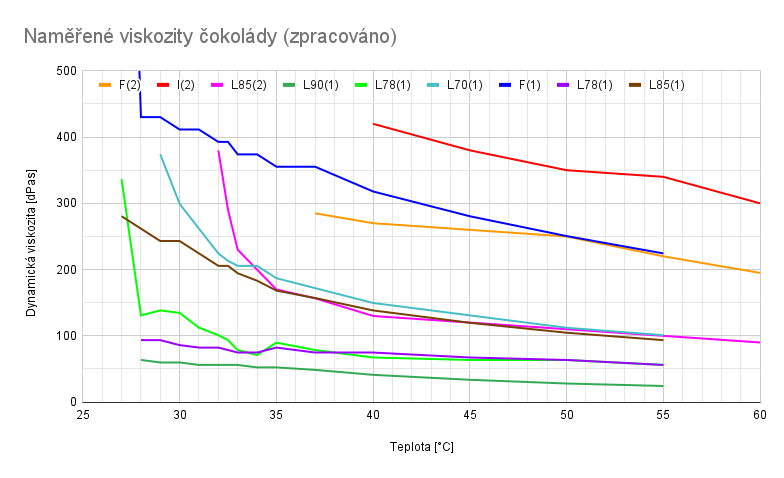
\includegraphics[width = \linewidth]{figures/data_zpracovano.png}
    \caption{Naměřené dynamické viskozity čokolád. Pro druhy čokolád viz tabulku č.~\ref{tab:cokolady} v~příloze. Číslo v~závorce udává vřeteno použité k~měření (viz tabulku vřeten, str.~\pageref{tab:vretena}). Hodnoty naměřené vřetenem č.~1 jsou přepočteny pomocí vztahu~\ref{eq:prepocet} popsaného na str.~\pageref{eq:prepocet}. Vytvořeno s~pomocí Tabulek Google.}
    \label{fig:data_zprac}
\end{figure}

%%%%%%%%%%%%%%%%%%%%%%%%%%%%%%%%%%%%%%%%%%%%%%%%%%%%%%%%%%%%%%%%%%%%%%
\newpage%%%%%%%%%%%%%%%%%%%%%%%%%%%%%%%%%%%%%%%%%%%%%%%%%%%%%%%%%%%%%%
\section{Vyhodnocení a~diskuze}%%%%%%%%%%%%%%%%%%%%%%%%%%%%%%%%%%%%%%%
%%%%%%%%%%%%%%%%%%%%%%%%%%%%%%%%%%%%%%%%%%%%%%%%%%%%%%%%%%%%%%%%%%%%%%
%%%%%%%%%%%%%%%%%%%%%%%%%%%%%%%%%%%%%%%%%%%%%%%%%%%%%%%%%%%%%%%%%%%%%%

%%%%%%%%%%%%%%%%%%%%%%%%%%%%%%%%%%%%%%%%%%%%%%%%%%%%%%%%%%%%%%%%%%%%%%
\subsection{Vyhodnocování výsledků}%%%%%%%%%%%%%%%%%%%%%%%%%%%%%%%%%%%
%%%%%%%%%%%%%%%%%%%%%%%%%%%%%%%%%%%%%%%%%%%%%%%%%%%%%%%%%%%%%%%%%%%%%%

Datový bod tvoří naměřená viskozita čokolády při určité naměřené teplotě lázně. V~případě, že bylo při stejné teplotě provedeno více měření, byl ze všech měření vypočítán aritmetický průměr a~za viskozitu čokolády při dané teplotě se považujte tato hodnota.

%%%%%%%%%%%%%%%%%%%%%%%%%%%%%%%%%%%%%%%%%%%%%%%%%%%%%%%%%%%%%%%%%%%%%%
\subsection{Srovnávání dat naměřených dvěma různými vřeteny}%%%%%%%%%%
%%%%%%%%%%%%%%%%%%%%%%%%%%%%%%%%%%%%%%%%%%%%%%%%%%%%%%%%%%%%%%%%%%%%%%

Hodnoty viskozity čokolády naměřené dvěma různými vřeteny nejsou přímo srovnatelné, a~to z~těchto důvodů:
\begin{itemize}[noitemsep, topsep = 0pt]
    \item \underline{\smash{Různá hloubka ponoru vřetena}}: Měřené množství čokolády (\SI{100}{\gram}) nestačí k~úplnému ponoření měřicího vřetena č.~1 (viz tabulku vřeten, str.~\pageref{tab:vretena}), vřeteno je v~čokoládě ponořeno zhruba z~poloviny. Naměřená viskozita tedy bude alespoň dvakrát menší, než její skutečná hodnota. 
    \item \underline{\smash{Měření je prováděné při různých rychlostech deformace}}: Vzhledem k~tomu, že jednotlivá vřetena mají různé poloměry (opět viz tabulku vřeten, str.~\pageref{tab:vretena}), bude měření různými vřeteny prováděno (dle vztahu~\ref{eq:viskozimetr_gamma} na straně~\pageref{eq:viskozimetr_gamma}) při různých rychlostech deformace. Naměřená (zdánlivá) viskozita se tedy bude lišit, protože se nejedná o~newtonovskou kapalinu.
\end{itemize}
Mezi hloubkou ponoru vřetena a~naměřenou viskozitou by měl být, pokud zanedbáme tření s~horní podstavou válce, lineární vztah, a~tato chyba by tedy měla být jednoduše odstranitelná.
\par\noindent
Pro pseudoplastické vlastnosti čokolády můžeme tvrdit, že její zdánlivá viskozita se stoupající rychlostí deformace klesá. Zároveň budeme předpokládat, že podíl zdánlivých viskozit je konstantní napříč teplotním rozsahem (jelikož vztah~\ref{eq:viskozimetr_gamma} na teplotě ani zdánlivé viskozitě nezávisí).
\par\noindent
Bude tedy platit vztah:
\begin{equation}
    \eta_2 \approx k\eta_1\text{,}
    \label{eq:prepocet}
\end{equation}
kde $\eta_2$ je zdánlivá viskozita naměřená vřetenem č.~2, $\eta_1$ je zdánlivá viskozita naměřená vřetenem č.~1 a~$k$ je převodní koeficient.
\par\noindent
Pro zjištění hodnoty převodního koeficientu $k$ byly dvě čokolády se značně odlišnou viskozitou naměřeny oběma vřeteny. Konkrétně se jednalo o~čokoládu Figaro, která má oproti ostatním měřeným čokoládám relativně vysokou viskozitu, a~čokoládu Lindt 85\%, která má viskozitu relativně nízkou. Pro hodnoty, kde se tvary křivek viskozity shodovaly, byl spočten poměr naměřených hodnot. Touto metodou byla zjištěna hodnota koeficientu $k\approx 3,74$. Hodnoty použité k~výpočtu tohoto koeficientu jsou dostupné v~tabulce~\ref{tab:vypocet_koeficientu} v~příloze.
\par\noindent
Hodnoty naměřené vřetenem č.~1 byly před vyhodnocením a~srovnáváním s~daty naměřenými pomocí vřetena č.~2 přepočteny podle výše zmíněného vztahu.

%%%%%%%%%%%%%%%%%%%%%%%%%%%%%%%%%%%%%%%%%%%%%%%%%%%%%%%%%%%%%%%%%%%%%%
\subsection{Určení Cassonovy plastické viskozity z~naměřených dat}%%%%
%%%%%%%%%%%%%%%%%%%%%%%%%%%%%%%%%%%%%%%%%%%%%%%%%%%%%%%%%%%%%%%%%%%%%%

Z~naměřených dat je možné vypočítat Cassonovu plastickou viskozitu $\eta_{CA}$ a~Cassonovo prahové napětí $\tau_{CA}$ (pro vysvětlení viz kapitolu Cassonův model, str.~\pageref{sec:Casson}). Viskozimetrem jsme změřili zdánlivou viskozitu $\eta(\dot\gamma)$, rychlost deformace je určená vztahem~\ref{eq:viskozimetr_gamma} (str.~\pageref{eq:viskozimetr_gamma}) a~tečné napětí $\tau$ pak lze odvodit ze vztahu~\ref{eq:zdanliva_viskozita} (str.~\pageref{eq:zdanliva_viskozita}). V~Cassonově modelu (vztah~\ref{eq:Casson_model}, str.~\pageref{eq:Casson_model}) nám pak zbývají pouze ony dvě hledané proměnné. U~čokolád, které byly měřeny dvěma vřeteny, tak můžeme sestavit následující soustavu rovnic:
\begin{equation}
    \begin{cases}
        \sqrt{\tau_1} = \sqrt{\tau_{CA}} + \sqrt{\eta_{CA}\cdot\dot\gamma_1}\text{,}\\
        \sqrt{\tau_2} = \sqrt{\tau_{CA}} + \sqrt{\eta_{CA}\cdot\dot\gamma_2}\text{,}
    \end{cases}
\end{equation}
kde $\tau_i$ je obecně tečné napětí naměřené vřetenem č.~$i$, pro které platí $\tau_i = \dot\gamma_i\cdot\eta(\dot\gamma_i)$. Vzhledem k~tomu, že se vřetena otáčejí známou úhlovou rychlostí (výrobce udává $62,5\:\frac{\text{ot.}}{\SI{}{\minute}}$)~\cite{man:VT-02}, a~že výrobce udává průměr kádinky 52,6\SI{\pm 0,25}{\milli\metre}~\cite{man:VT-02}, lze spočítat rychlosti deformace pro jednotlivá vřetena dle vztahu~\ref{eq:viskozimetr_gamma}:
\begin{align}
    \begin{split}
        \dot\gamma(R_{v1}) =& \frac{2\Omega R^2}{(R^2-R_v^2)} = \frac{2\cdot\SI{6,5450}{\radian\per\second}\cdot\SI{5,5696e-4}{\metre\squared}}{\SI{4,1296e-4}{\metre\squared}} = \frac{\SI{72,906}{\radian\metre\squared\per\second}}{\SI{4,1296}{\metre\squared}} =\\ =& \SI{17,654}{\radian\per\second}\text{,}\\
        \dot\gamma(R_{v2}) =& \frac{2\Omega R^2}{(R^2-R_v^2)} = \frac{2\cdot\SI{6,5450}{\radian\per\second}\cdot\SI{5,5696e-4}{\metre\squared}}{\SI{5,0071e-4}{\metre\squared}} = \frac{\SI{72,906}{\radian\metre\squared\per\second}}{\SI{5,0071}{\metre\squared}} =\\ =& \SI{14,561}{\radian\per\second}\text{.}
    \end{split}
\end{align}
Z~naměřených hodnot se lze dopočítat k~tečným napětím (viz tabulku~\ref{tab:vypocet_casson} v~příloze). Dosazením a~vyřešením soustav rovnic lze získat Cassonovu plastickou viskozitu $\eta_{CA}$ a~Cassonovo prahové napětí $\tau_{CA}$ při různých teplotách -- tyto jsou uvedeny v~tabulce~\ref{tab:vysledky_casson}.
\begin{table}[h!]
    \centering
    \begin{tabular}{|c|c c|c c|}
        \hline
        & \multicolumn{2}{c|}{Lindt 85\%} & \multicolumn{2}{c|}{Figaro}\\
        Teplota [\SI{}{\degreeCelsius}] & $\eta_{CA}$ & $\tau_{CA}$ & $\eta_{CA}$ & $\tau_{CA}$ \\\hline
        32 & $\nexists$ & $\nexists$ & &\\
        32,5 & $\nexists$ & $\nexists$ & &\\
        33 & 3,5 & 257 & & \\
        34 & 57,1 & 63 & & \\
        35 & 152,0 & 0,74 & & \\
        37 & $\nexists$ & $\nexists$ & $\nexists$ & $\nexists$\\
        40 & $\nexists$ & $\nexists$ & $\nexists$ & $\nexists$\\
        45 & 117 & 0,037 & $\nexists$ & $\nexists$\\
        50 & 59,5 & 11 & $\nexists$ & $\nexists$\\
        55 & 41,0 & 19 & $\nexists$ & $\nexists$\\\hline 
    \end{tabular}
    \caption{Cassonova plastická viskozita [\SI{}{\deci\pascal\second}] a~Cassonovo prahové napětí [\SI{}{\pascal}]. Pokud řešení soustavy rovnic neexistuje, je použit znak~$\nexists$. Data použitá k~výpočtu jsou v~tabulce~\ref{tab:vypocet_casson} v~příloze.}
    \label{tab:vysledky_casson}
\end{table}
\par\noindent
Hodnoty, ke kterým jsme tímto postupem dospěli, buď nedávají smysl nebo vůbec neexistují. Toto je nejspíš způsobeno vstupními hodnotami zdánlivé viskozity, která byla měřená vřetenem č.~1. Vřeteno č.~1 nebylo plně ponořeno, naměřené hodnoty tedy nelze použít přímo a~je nutné je přepočítávat postupem, který je popsán v~předchozí podkapitole. Tyto přepočtené výsledky už jsou (skrze koeficient $k$) závislé na údajích naměřených vřetenem č.~2. I~malé změny tohoto koeficientu značným způsobem ovlivní řešení použité soustavy rovnic. Aby byla tato metoda použitelná, bylo by nutné měřit oběma vřeteny plnou kádinku čokolády, což by bylo časově ještě náročnější.
\par\noindent
I~přesto, že by měly být výsledné hodnoty naprosto nesprávné, odpovídají (obzvláště u~vyšších teplot) alespoň řádově hodnotám uváděných v~odborné literatuře. To je však jistě alespoň částečně způsobeno tím, v~jakých řádech se pohybují vstupní hodnoty. Cassonova plastická viskozita čokolády se řádově pohybuje v~jednotkách až desítkách \SI{}{\deci\pascal\second}, Cassonovo prahové napětí se řádově pohybuje v~desítkách \SI{}{\pascal}.~\cite{Article:Rapid_and_economic_chocolate_viscosity}\cite{Article:viscosity_molten_milk_chocolate}\cite{Article:chocolate_shear_stress}

%%%%%%%%%%%%%%%%%%%%%%%%%%%%%%%%%%%%%%%%%%%%%%%%%%%%%%%%%%%%%%%%%%%%%%
\subsection{Anomálie v~datech}%%%%%%%%%%%%%%%%%%%%%%%%%%%%%%%%%%%%%%%%
%%%%%%%%%%%%%%%%%%%%%%%%%%%%%%%%%%%%%%%%%%%%%%%%%%%%%%%%%%%%%%%%%%%%%%

\subsubsection{Viskozita čokolády Lindt 78\% při nízkých teplotách}%%%

Při měření první várky čokolády Lindt 78\% naměřené viskozity neodpovídaly \glqq pěkné\grqq křivce, jako tomu bylo u~ostatních naměřených čokolád, ale měnily se poněkud náhodně (viskozita s~klesající teplotou i~klesala). Z~tohoto důvodu byla později měřena nová várka této čokolády. I~tyto nové hodnoty vykazovaly podobné anomální chování. Data těchto dvou měření a~jejich průměr jsou zaneseny v~grafu na obrázku \ref{fig:Lindt_78_anomalie}. Nejzřetelnější anomálií je propad viskozity mezi 32 a~\SI{35}{\degreeCelsius}, další anomálií je pokles viskozity při poklesu teploty z~29 na \SI{28}{\degreeCelsius}.
\par\noindent
Příčina tohoto jevu zůstává neznámá. Nejspíše je pokles viskozity způsoben nehomogenním prohřátím čokoládové taveniny a~krystalizací a~opětovným táním kakaového másla při míchání čokolády. Jelikož není možné zajistit totožné podmínky promíchávání a~zahřívání čokolády při těchto teplotách, nepovažuji tento problém za odstranitelný. Mechanismus rozcházejících se dat bude jistě souviset i~s principy popsanými v~následující podkapitole.

\begin{figure}[h!]
    \centering
    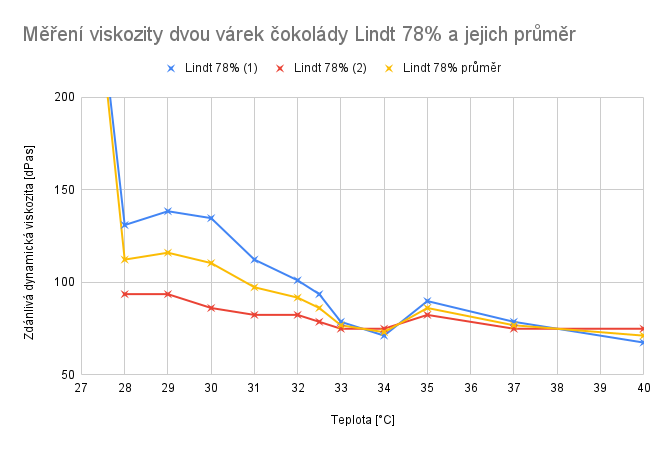
\includegraphics[width = \linewidth]{figures/Lindt78.png}
    \caption{Anomální data viskozity čokolády Lindt 78\%. Modře jsou vynesena data naměřená při prvním pokusu, oranžově jsou vyznačena data naměřená při druhém pokusu, žlutě je vynesena průměrná hodnota těchto dvou měření. Měřeno pomocí měřicího vřetena č.~1, hodnoty viskozity jsou přepočteny s~převodním koeficientem $k = 3,74$. Data dostupná v~tabulce \ref{tab:data_anomalie_lindt_78} v~příloze. Vytvořeno pomocí Tabulek Google.}
    \label{fig:Lindt_78_anomalie}
\end{figure}

\subsubsection{Odlišné teploty tuhnutí čokolády při různých měřeních}%

Při měření čokolády Lindt 85\% byly u~dvou různých várek naměřeny dva rozdílné body tání. Podobně u~čokolády Lindt 78\% byly při měření zjištěny odlišné průběhy viskozity při nízkých teplotách. Rozdíl mezi datovými řadami je graficky znázorněn na obrázku~\ref{fig:coko_nizke_teploty}.

\begin{figure}
    \centering
    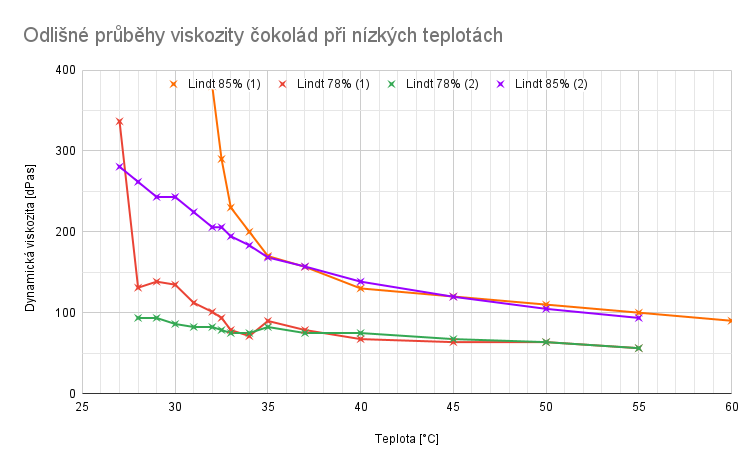
\includegraphics[width = \linewidth]{figures/coko_nizke_teploty.png}
    \caption{Odlišné průběhy dynamických viskozit čokolád při nízkých teplotách. Data měřená různými vřeteny, přepočteno. Vytvořeno s~pomocí Tabulek Google.}
    \label{fig:coko_nizke_teploty}
\end{figure}
\par\noindent

To, že se datové řady rozcházejí nejspíše souvisí s~jevem, který je popsán již v~zadání úlohy Turnaje mladých fyziků (str.~\pageref{sec:zadani_tmf}). Pro polymorfní vlastnosti kakaového másla (popsané na str.~\pageref{sec:polymorfie}) nejspíše čokoládová tavenina při nízkých teplotách postupně částečně krystalizovala, poměry zastoupení jednotlivých polymorfů však mohly být různé. Krystalizace mohla být ovlivněna tím, jak dlouho a~na jaké teploty byla čokoládová tavenina zahřívána a~jak často a~s jakou důsledností byla čokoláda míchána. Pro nerovnoměrné prohřátí čokolády mohla studenější část začít krystalizovat, při promíchání naopak tát, a~struktura čokoládové taveniny tedy mohla být nehomogenní. Zajistit však, aby všechny čokoládové vzorky prošly naprosto totožnými podmínkami co se teploty a~míchání týče, považuji za nemožné.

\subsubsection{Rozdíly v~hodnotách naměřených vřeteny č. 1 a~2}%%%%%%%

Data naměřená různými měřicími vřeteny se rozcházejí, obzvláště při nízkých teplotách. Tento jev je zobrazen na obrázku \ref{fig:ruzna_vretena}. Kromě principů popsaných výše zde může hrát roli i~rozdílná rychlost deformace, při které je měření prováděno. Kromě standardních jevů pseudoplasticity zde může docházet k~prokluzování měřicího vřetena v~čokoládě, kdy mezní vrstva nepřiléhá dokonale k~povrchu vřetena a~moment síly působící na vřeteno je tedy nižší. 

\begin{figure}
    \centering
    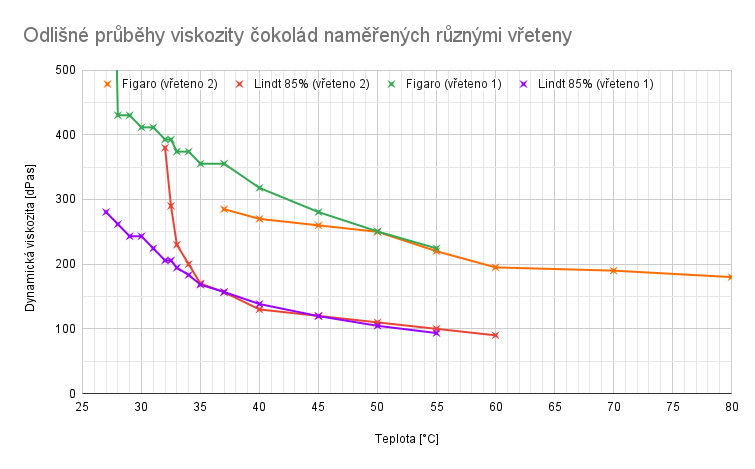
\includegraphics[width = \linewidth]{figures/ruzna_vretena.png}
    \caption{Datové řady čokolád naměřených různými vřeteny. Vytvořeno s~pomocí Tabulek Google.}
    \label{fig:ruzna_vretena}
\end{figure}

%%%%%%%%%%%%%%%%%%%%%%%%%%%%%%%%%%%%%%%%%%%%%%%%%%%%%%%%%%%%%%%%%%%%%%
\newpage%%%%%%%%%%%%%%%%%%%%%%%%%%%%%%%%%%%%%%%%%%%%%%%%%%%%%%%%%%%%%%
\section{Závěr}%%%%%%%%%%%%%%%%%%%%%%%%%%%%%%%%%%%%%%%%%%%%%%%%%%%%%%%
%%%%%%%%%%%%%%%%%%%%%%%%%%%%%%%%%%%%%%%%%%%%%%%%%%%%%%%%%%%%%%%%%%%%%%
%%%%%%%%%%%%%%%%%%%%%%%%%%%%%%%%%%%%%%%%%%%%%%%%%%%%%%%%%%%%%%%%%%%%%%

Oblast proudění a~tečení kapalin (mechanika kontinua) se ukázala být složitějším vědním oborem, než se na první pohled zdálo. Popravdě se nedivím, že se žádnému učiteli téma viskozity probírat nechce.
\par\noindent
Reologické vlastnosti čokolády se také ukázaly jako netriviální.
\par\noindent
Z navrhovaných měřicích metod se měření rotačním viskozimetrem ukázalo jako nejvhodnější. V~porovnání s~ostatními uvažovanými měřicími metodami je v~zásadě poměrně nenáročné. Měření kapilárním nebo nálevkovým viskozimetrem by se teoreticky také nabízelo (u~čokolád s~nižší viskozitou), bylo by však nutné sehnat vhodné měřicí pomůcky.
\par\noindent
Sestavená měřicí aparatura fungovala po vyřešení všech popsaných problémů spolehlivě. Měření byla ve vyšším rozsahu teplot opakovatelná -- v~nižším rozsahu převládne náhodnost vlivů okolí na krystalizaci kakaového másla a~reologické vlastnosti jednotlivých várek téže čokolády se liší.
\par\noindent
Výsledky měření jsou v~naprosté většině případů smysluplné a~uspokojivé. Nesrovnalosti ve výsledcích jsou způsobené výše popsanými neovlivnitelnými náhodnými vlivy. Ke zvýšení relevance výsledků by bylo vhodné měřit větší objemy čokolády vždy dvěma vřeteny, aby bylo možné dospět (i~s~použitím této levné a~technicky poměrně nenáročné metody) k~hodnotám Cassonovy plastické viskozity a~Cassonova prahového napětí. Teoreticky to možné je a~umožnilo by to lépe srovnat výsledky měření s~odbornou literaturou. Dle mého názoru se jedná se o~vhodný předmět dalšího zkoumání.

%%%%%%%%%%%%%%%%%%%%%%%%%%%%%%%%%%%%%%%%%%%%%%%%%%%%%%%%%%%%%%%%%%%%%%
\newpage%%%%%%%%%%%%%%%%%%%%%%%%%%%%%%%%%%%%%%%%%%%%%%%%%%%%%%%%%%%%%%
\section*{Reference}%%%%%%%%%%%%%%%%%%%%%%%%%%%%%%%%%%%%%%%%%%%%%%%%%%
\addcontentsline{toc}{section}{Reference}%%%%%%%%%%%%%%%%%%%%%%%%%%%%%
%%%%%%%%%%%%%%%%%%%%%%%%%%%%%%%%%%%%%%%%%%%%%%%%%%%%%%%%%%%%%%%%%%%%%%

\printbibliography[heading=none]

\newpage%%%%%%%%%%%%%%%%%%%%%%%%%%%%%%%%%%%%%%%%%%%%%%%%%%%%%%%%%%%%%%
\pagestyle{empty}%%%%%%%%%%%%%%%%%%%%%%%%%%%%%%%%%%%%%%%%%%%%%%%%%%%%%
\section*{Přílohy}%%%%%%%%%%%%%%%%%%%%%%%%%%%%%%%%%%%%%%%%%%%%%%%%%%%%
\addcontentsline{toc}{section}{Přílohy}%%%%%%%%%%%%%%%%%%%%%%%%%%%%%%%
%%%%%%%%%%%%%%%%%%%%%%%%%%%%%%%%%%%%%%%%%%%%%%%%%%%%%%%%%%%%%%%%%%%%%%

%%%%%%%%%%%%%%%%%%%%%%%%%%%%%%%%%%%%%%%%%%%%%%%%%%%%%%%%%%%%%%%%%%%%%%
\subsection*{Seznam příloh}%%%%%%%%%%%%%%%%%%%%%%%%%%%%%%%%%%%%%%%%%%%
%%%%%%%%%%%%%%%%%%%%%%%%%%%%%%%%%%%%%%%%%%%%%%%%%%%%%%%%%%%%%%%%%%%%%%

\begin{enumerate}[noitemsep, topsep = 0pt]
    \item Tabulka měřených čokolád
    \item Data pro výpočet převodního koeficientu $k$
    \item Data naměřená vřetenem č. 2
    \item Data naměřená vřetenem č. 1
    \item Přepočtené a~zprůměrované hodnoty viskozit pro jednotlivé druhy čokolády
    \item Data k~výpočtu Cassonovy plastické viskozity a~Cassonova prahového napětí
    \item Data použita na obrázku \ref{fig:Lindt_78_anomalie}
    \item Odkazy
    \item Obrázky
\end{enumerate}

\newpage%%%%%%%%%%%%%%%%%%%%%%%%%%%%%%%%%%%%%%%%%%%%%%%%%%%%%%%%%%%%%%
\subsection*{Příloha č. 1: Tabulka měřených čokolád}%%%%%%%%%%%%%%%%%%
%%%%%%%%%%%%%%%%%%%%%%%%%%%%%%%%%%%%%%%%%%%%%%%%%%%%%%%%%%%%%%%%%%%%%%

\begin{table}[!h]
    \centering
    \begin{NiceTabular}{|c|c|}
        \hline
        Název čokolády & Použitá zkratka \\ \hline\hline
        Figaro čokoláda na vaření & F \\ \hline
        Ikea milk chocolate & I \\ \hline
        Lindt Excellence 70\% cocoa & L70 \\ \hline
        Lindt Excellence 78\% cocoa & L78 \\ \hline
        Lindt Excellence 85\% cocoa & L85 \\ \hline
        Lindt Excellence 90\% cocoa & L90 \\      
        \hline
    \end{NiceTabular}
    \caption{Tabulka měřených čokolád}
    \label{tab:cokolady}
\end{table} %Tabulka čokolád

%%%%%%%%%%%%%%%%%%%%%%%%%%%%%%%%%%%%%%%%%%%%%%%%%%%%%%%%%%%%%%%%%%%%%%
\subsection*{Příloha č. 2: Data pro výpočet převodního koeficientu $k$}
%%%%%%%%%%%%%%%%%%%%%%%%%%%%%%%%%%%%%%%%%%%%%%%%%%%%%%%%%%%%%%%%%%%%%%

\begin{table}[!h]
    \centering
    \begin{tabular}{|c|c c|c c|}
        \hline
        & \multicolumn{2}{c|}{Lindt 85\% [\SI{}{\deci\pascal\second}]} & \multicolumn{2}{c|}{Figaro [\SI{}{\deci\pascal\second}]}\\
        Teplota [\SI{}{\degreeCelsius}] & Vřeteno 1 & Vřeteno 2 & Vřeteno 1 & Vřeteno 2 \\\hline
        35 & 45 & 170 & & \\
        37 & 42 & 156,\overline{6} & & \\
        40 & 37 & 130 & & \\
        45 & 32 & 120 & & \\
        50 & 28 & 110 & 67 & 250 \\
        55 & 25 & 100 & 60 & 220 \\\hline
        Součet & 209 & 786,\overline{6} & 127 & 470 \\\hline        
    \end{tabular}
    \caption{Data použitá pro výpočet převodního koeficientu $k$, viz str.~\pageref{eq:prepocet}.}
    \label{tab:vypocet_koeficientu}
\end{table}
$$k = \frac{789,\overline{6} + 470}{209 + 127} = \frac{1256,\overline{6}}{336} \doteq 3,74\text{.}$$

\newpage%%%%%%%%%%%%%%%%%%%%%%%%%%%%%%%%%%%%%%%%%%%%%%%%%%%%%%%%%%%%%%
\subsection*{Příloha č. 3: Data naměřená vřetenem č. 2}%%%%%%%%%%%%%%%
%%%%%%%%%%%%%%%%%%%%%%%%%%%%%%%%%%%%%%%%%%%%%%%%%%%%%%%%%%%%%%%%%%%%%%

\begin{table}[h!]
    \centering
    \begin{NiceTabular}{|c|c|c|c|c|c|c|}
        \hline
        \rule[-10mm]{24mm}{0cm}
        \diagbox{Teplota[\SI{}{\degreeCelsius}]}{Čokoláda}
        &\Block{}{\\F}
        &\Block{}{\\F}
        &\Block{}{\\I}
        &\Block{}{\\L85}
        &\Block{}{\\L85}
        &\Block{}{\\L85}
        \\\hline
        31 & & & & & & tuhé\\
        32 & & & & & & 380\\
        32,5 & & & & & 290 &\\
        33 & & & & & & 230\\
        34 & & & & & & 200\\
        35  & & & & & 170 &\\
        37 & 290 & 280 & & 170 & 150 & 150\\
        40 & 280 & 260 & 420 & 130 & &\\
        45 & 270 & 250 & 380 & 120 & &\\
        50 & 250 & 250 & 350 & 110 & &\\
        55 & 220 & 220 & 340 & 100 & &\\
        60 & 200 & 190 & 300 & 90 & &\\
        70 & 190\\
        80 & 180\\
        \hline
    \end{NiceTabular}
    \caption{Hodnoty dynamických viskozit [\SI{}{\deci\pascal\second}] měřené pomocí vřetena č.~2 (viz tabulku vřeten, str.~\pageref{tab:vretena}). Každý sloupec představuje jednu várku čokolády. Pro zkratky čokolád viz tabulku~\ref{tab:cokolady}.}
    \label{tab:data_raw_dpas2}
\end{table}

%%%%%%%%%%%%%%%%%%%%%%%%%%%%%%%%%%%%%%%%%%%%%%%%%%%%%%%%%%%%%%%%%%%%%%
\subsection*{Příloha č. 4: Data naměřená vřetenem č. 1}%%%%%%%%%%%%%%%
%%%%%%%%%%%%%%%%%%%%%%%%%%%%%%%%%%%%%%%%%%%%%%%%%%%%%%%%%%%%%%%%%%%%%%

\begin{table}[h!]
    \centering
    \begin{NiceTabular}{|c|c|c|c|c|c|c|c|c|c|c|}
        \hline
        \rule[-10mm]{24mm}{0cm}
        \diagbox{Teplota[\SI{}{\degreeCelsius}]}{Čokoláda}
        &\Block{}{\\L90}
        &\Block{}{\\L90}
        &\Block{}{\\L78}
        &\Block{}{\\L70}
        &\Block{}{\\L70}
        &\Block{}{\\F}
        &\Block{}{\\L78}
        &\Block{}{\\L78}
        &\Block{}{\\L85}
        &\Block{}{\\L85}
        \\\hline
        27 & & tuhé & 90 & & & & & tuhé & & 75\\
        28 & & 17 & 35 & & tuhé & 115 & & 25 & & 70\\
        29 & & 16 & 37 & & 100 & 115 & & 25 & & 65\\
        30 & & 16 & 36 & & 80 & 110 & & 23 & & 65\\
        31 & & 15 & 30 & & 70 & 110 & & 22 & & 60\\
        32 & & 15 & 27 & & 60 & 105 & & 22 & & 55\\
        32,5 & & 15 & 25 & & 57 & 105 & & 21 & & 55\\
        33 & & 15 & 21 & & 55 & 100 & & 20 & & 52\\
        34 & & 14 & 19 & & 55 & 100 & & 20 & & 49\\
        35 & & 14 & 24 & & 50 & 95 & & 22 & & 45\\
        37 & 14 & 12 & 21 & 47 & 45 & 95 & 22 & 20 & 41 & 43\\
        40 & 11 & & 18 & 40 & & 85 & 20 & & 37\\
        45 & 9 & & 17 & 35 & & 75 & 18 & & 32\\
        50 & 7,5 & & 17 & 30 & & 67 & 17 & & 28\\
        55 & 6,5 & & 15 & 27 & & 60 & 15 & & 25\\
        \hline
    \end{NiceTabular}
    \caption{Hodnoty dynamických viskozit [\SI{}{\deci\pascal\second}] měřené pomocí vřetena č.~2 (viz tabulku vřeten, str.~\pageref{tab:vretena}). Každý sloupec představuje jednu várku čokolády. Pro zkratky čokolád viz tabulku~\ref{tab:cokolady}.}
    \label{tab:data_raw_dpas1}
\end{table}

%%%%%%%%%%%%%%%%%%%%%%%%%%%%%%%%%%%%%%%%%%%%%%%%%%%%%%%%%%%%%%%%%%%%%%
\subsection*{Příloha č. 5: Přepočtené a~zprůměrované hodnoty viskozit pro jednotlivé druhy čokolády}
%%%%%%%%%%%%%%%%%%%%%%%%%%%%%%%%%%%%%%%%%%%%%%%%%%%%%%%%%%%%%%%%%%%%%%

\begin{table}[h!]
    \centering
    \begin{NiceTabular}{|c|c|c|c|c|c|c|}
        \hline
        \rule[-10mm]{24mm}{0cm}
        \diagbox{Teplota[\SI{}{\degreeCelsius}]}{Čokoláda}
        &\Block{}{\\F}
        &\Block{}{\\I}
        &\Block{}{\\L90}
        &\Block{}{\\L85}
        &\Block{}{\\L78}
        &\Block{}{\\L70}
        \\\hline
        27 & & & 280,1 & & 336,6\\
        28 & 430,1 & & 63,58 & 261,8 & 112,2\\
        29 & 430,1 & & 59,84 & 243,1 & 115,9 & 374\\
        30 & 411,4 & & 59,84 & 243,1 & 110,3 & 299,2\\
        31 & 411,4 & & 56,1 & 224,4 & 97,2 & 261,8\\
        32 & 392,7 & & 56,1 & 292,9 & 91,6 & 224,4\\
        32,5 & 392,7 & & 56,1 & 247,9 & 86,0 & 213,2\\
        33 & 374 & & 56,1 & 212,2 & 76,7 & 205,7\\
        34 & 374 & & 52,36 & 191,6 & 72,9 & 205,7\\
        35 & 355,3 & & 52,36 & 169,2 & 86,0 & 187\\
        37 & 308,4 & & 48,62 & 156,8 & 78,5 & 172,0\\
        40 & 286,0 & 420 & 41,14 & 134,2 & 71,1 & 149,6\\
        45 & 266,9 & 380 & 33,66 & 119,8 & 65,5 & 130,9\\
        50 & 250,2 & 350 & 28,05 & 107,4 & 63,6 & 112,2\\
        55 & 221,5 & 340 & 24,31 & 96,8 & 56,1 & 101,0\\
        60 & 195 & 300 & & 90\\
        70 & 190 & \\
        80 & 180 &\\
        \hline
    \end{NiceTabular}
    \caption{Přepočtené a~zprůměrované hodnoty dynamických viskozit [\SI{}{\deci\pascal\second}] čokolád. Pro zkratky čokolád viz tabulku~\ref{tab:cokolady}.}
    \label{tab:data_prepoctene}
\end{table}

\newpage%%%%%%%%%%%%%%%%%%%%%%%%%%%%%%%%%%%%%%%%%%%%%%%%%%%%%%%%%%%%%%
\subsection*{Příloha č. 6: Data k~výpočtu Cassonovy plastické viskozity a~Cassonova prahového napětí}
%%%%%%%%%%%%%%%%%%%%%%%%%%%%%%%%%%%%%%%%%%%%%%%%%%%%%%%%%%%%%%%%%%%%%%

\begin{table}[h!]
    \centering
    \begin{tabular}{|c|c c c c|c c c c|}
        \hline
        & \multicolumn{4}{c|}{Lindt 85\%} & \multicolumn{4}{c|}{Figaro}\\
        Teplota [\SI{}{\degreeCelsius}] & $\eta(\dot\gamma_1)$ & $\tau_1$ & $\eta(\dot\gamma_2)$ & $\tau_2$ & $\eta(\dot\gamma_1)$ & $\tau_1$ & $\eta(\dot\gamma_2)$ & $\tau_2$ \\\hline
        32 & 205,7 & 363 & 380 & 553 & & & &\\
        32,5 & 205,7 & 363 & 290 & 422 & & & &\\
        33 & 194,5 & 343 & 230 & 335 & & & &\\
        34 & 183,3 & 323 & 200 & 291 & & & &\\
        35 & 168,3 & 297 & 170 & 248 & & & &\\
        37 & 157,1 & 277 & 156,7 & 228 & 355,3 & 627 & 285 & 415\\
        40 & 138,4 & 244 & 130 & 189 & 317,9 & 561 & 270 & 393\\
        45 & 119,7 & 211 & 120 & 175 & 280,5 & 495 & 260 & 379\\
        50 & 104,7 & 185 & 110 & 160 & 250,6 & 422 & 250 & 364\\
        55 & 93,5 & 165 & 100 & 146 & 224,4 & 396 & 220 & 320\\\hline 
    \end{tabular}
    \caption{Data použitá pro řešení soustavy rovnic k~nalezení Cassonovy plastické viskozity a~Cassonova prahového napětí čokoládové taveniny v~tabulce~\ref{tab:vysledky_casson} na str.~\pageref{tab:vysledky_casson}. Zdánlivé viskozity uváděny v~\SI{}{\deci\pascal\second}, tečná napětí v~\SI{}{\pascal}.}
    \label{tab:vypocet_casson}
\end{table}

%%%%%%%%%%%%%%%%%%%%%%%%%%%%%%%%%%%%%%%%%%%%%%%%%%%%%%%%%%%%%%%%%%%%%%
\subsection*{Příloha č. 7: Data použita na obrázku~\ref{fig:Lindt_78_anomalie}}
%%%%%%%%%%%%%%%%%%%%%%%%%%%%%%%%%%%%%%%%%%%%%%%%%%%%%%%%%%%%%%%%%%%%%%

\begin{table}[h!]
    \centering
    \begin{NiceTabular}{|c|c|c|c|}
        \hline
        Teplota \SI{}{\degreeCelsius} & Várka 1 & Várka 2 & Průměr  \\\hline
        27 & 336,6 & & 336,6 \\
        28 & 130,9 & 93,5 & 112,2\\
        29 & 138,4 & 93,5 & 115,9\\
        30 & 134,6 & 86,0 & 110,3\\
        31 & 112,2 & 82,3 & 97,2 \\
        32 & 101,0 & 82,3 & 91,6\\
        32,5 & 93,5 & 78,5 & 86,0 \\
        33 & 78,5 & 74,8 & 76,7 \\
        34 & 71,1 & 74,8 & 72,9 \\
        35 & 89,8 & 82,3 & 86,0 \\
        37 & 78,5 & 78,5 & 78,5\\
        40 & 67,3 & 74,8 & 71,1\\
        45 & 63,6 & 67,3 & 65,5\\
        50 & 63,6 & 63,6 & 63,6\\
        55 & 56,1 & 56,1 & 56,1 \\
        \hline
    \end{NiceTabular}
    \caption{Data k~obrázku~\ref{fig:Lindt_78_anomalie}: naměřené dynamické viskozity [\SI{}{\deci\pascal\second}] čokolády Lindt 78\%.}
    \label{tab:data_anomalie_lindt_78}
\end{table}

\newpage%%%%%%%%%%%%%%%%%%%%%%%%%%%%%%%%%%%%%%%%%%%%%%%%%%%%%%%%%%%%%%
\subsection*{Příloha č. 8: Odkazy}%%%%%%%%%%%%%%%%%%%%%%%%%%%%%%%%%%%%
%%%%%%%%%%%%%%%%%%%%%%%%%%%%%%%%%%%%%%%%%%%%%%%%%%%%%%%%%%%%%%%%%%%%%%

\glqq Zdrojový kód\grqq\space této práce ve formátu~.tex, jakožto tabulka s~naměřenými daty, obrázky a~obecně všechny podklady k~této maturitní práci jsou k~nalezení v~gitovém repozitáři na adrese:\\\url{https://github.com/Xichtik/Maturitni-prace-Viskozita-cokolady.git}
\par\noindent
Samotná Google tabulka s~naměřenými daty je dostupná na adrese: \url{https://docs.google.com/spreadsheets/d/1aIXDNuHhVtbhjn-V-A5yoDLF0yB9g1KJuwBW0kRpuE4/edit?usp=sharing}

\newpage%%%%%%%%%%%%%%%%%%%%%%%%%%%%%%%%%%%%%%%%%%%%%%%%%%%%%%%%%%%%%%
\subsection*{Příloha č. 9: Obrázky}%%%%%%%%%%%%%%%%%%%%%%%%%%%%%%%%%%%
%%%%%%%%%%%%%%%%%%%%%%%%%%%%%%%%%%%%%%%%%%%%%%%%%%%%%%%%%%%%%%%%%%%%%%

\begin{figure}[h!]
    \begin{subfigure}[b]{.5\textwidth}
        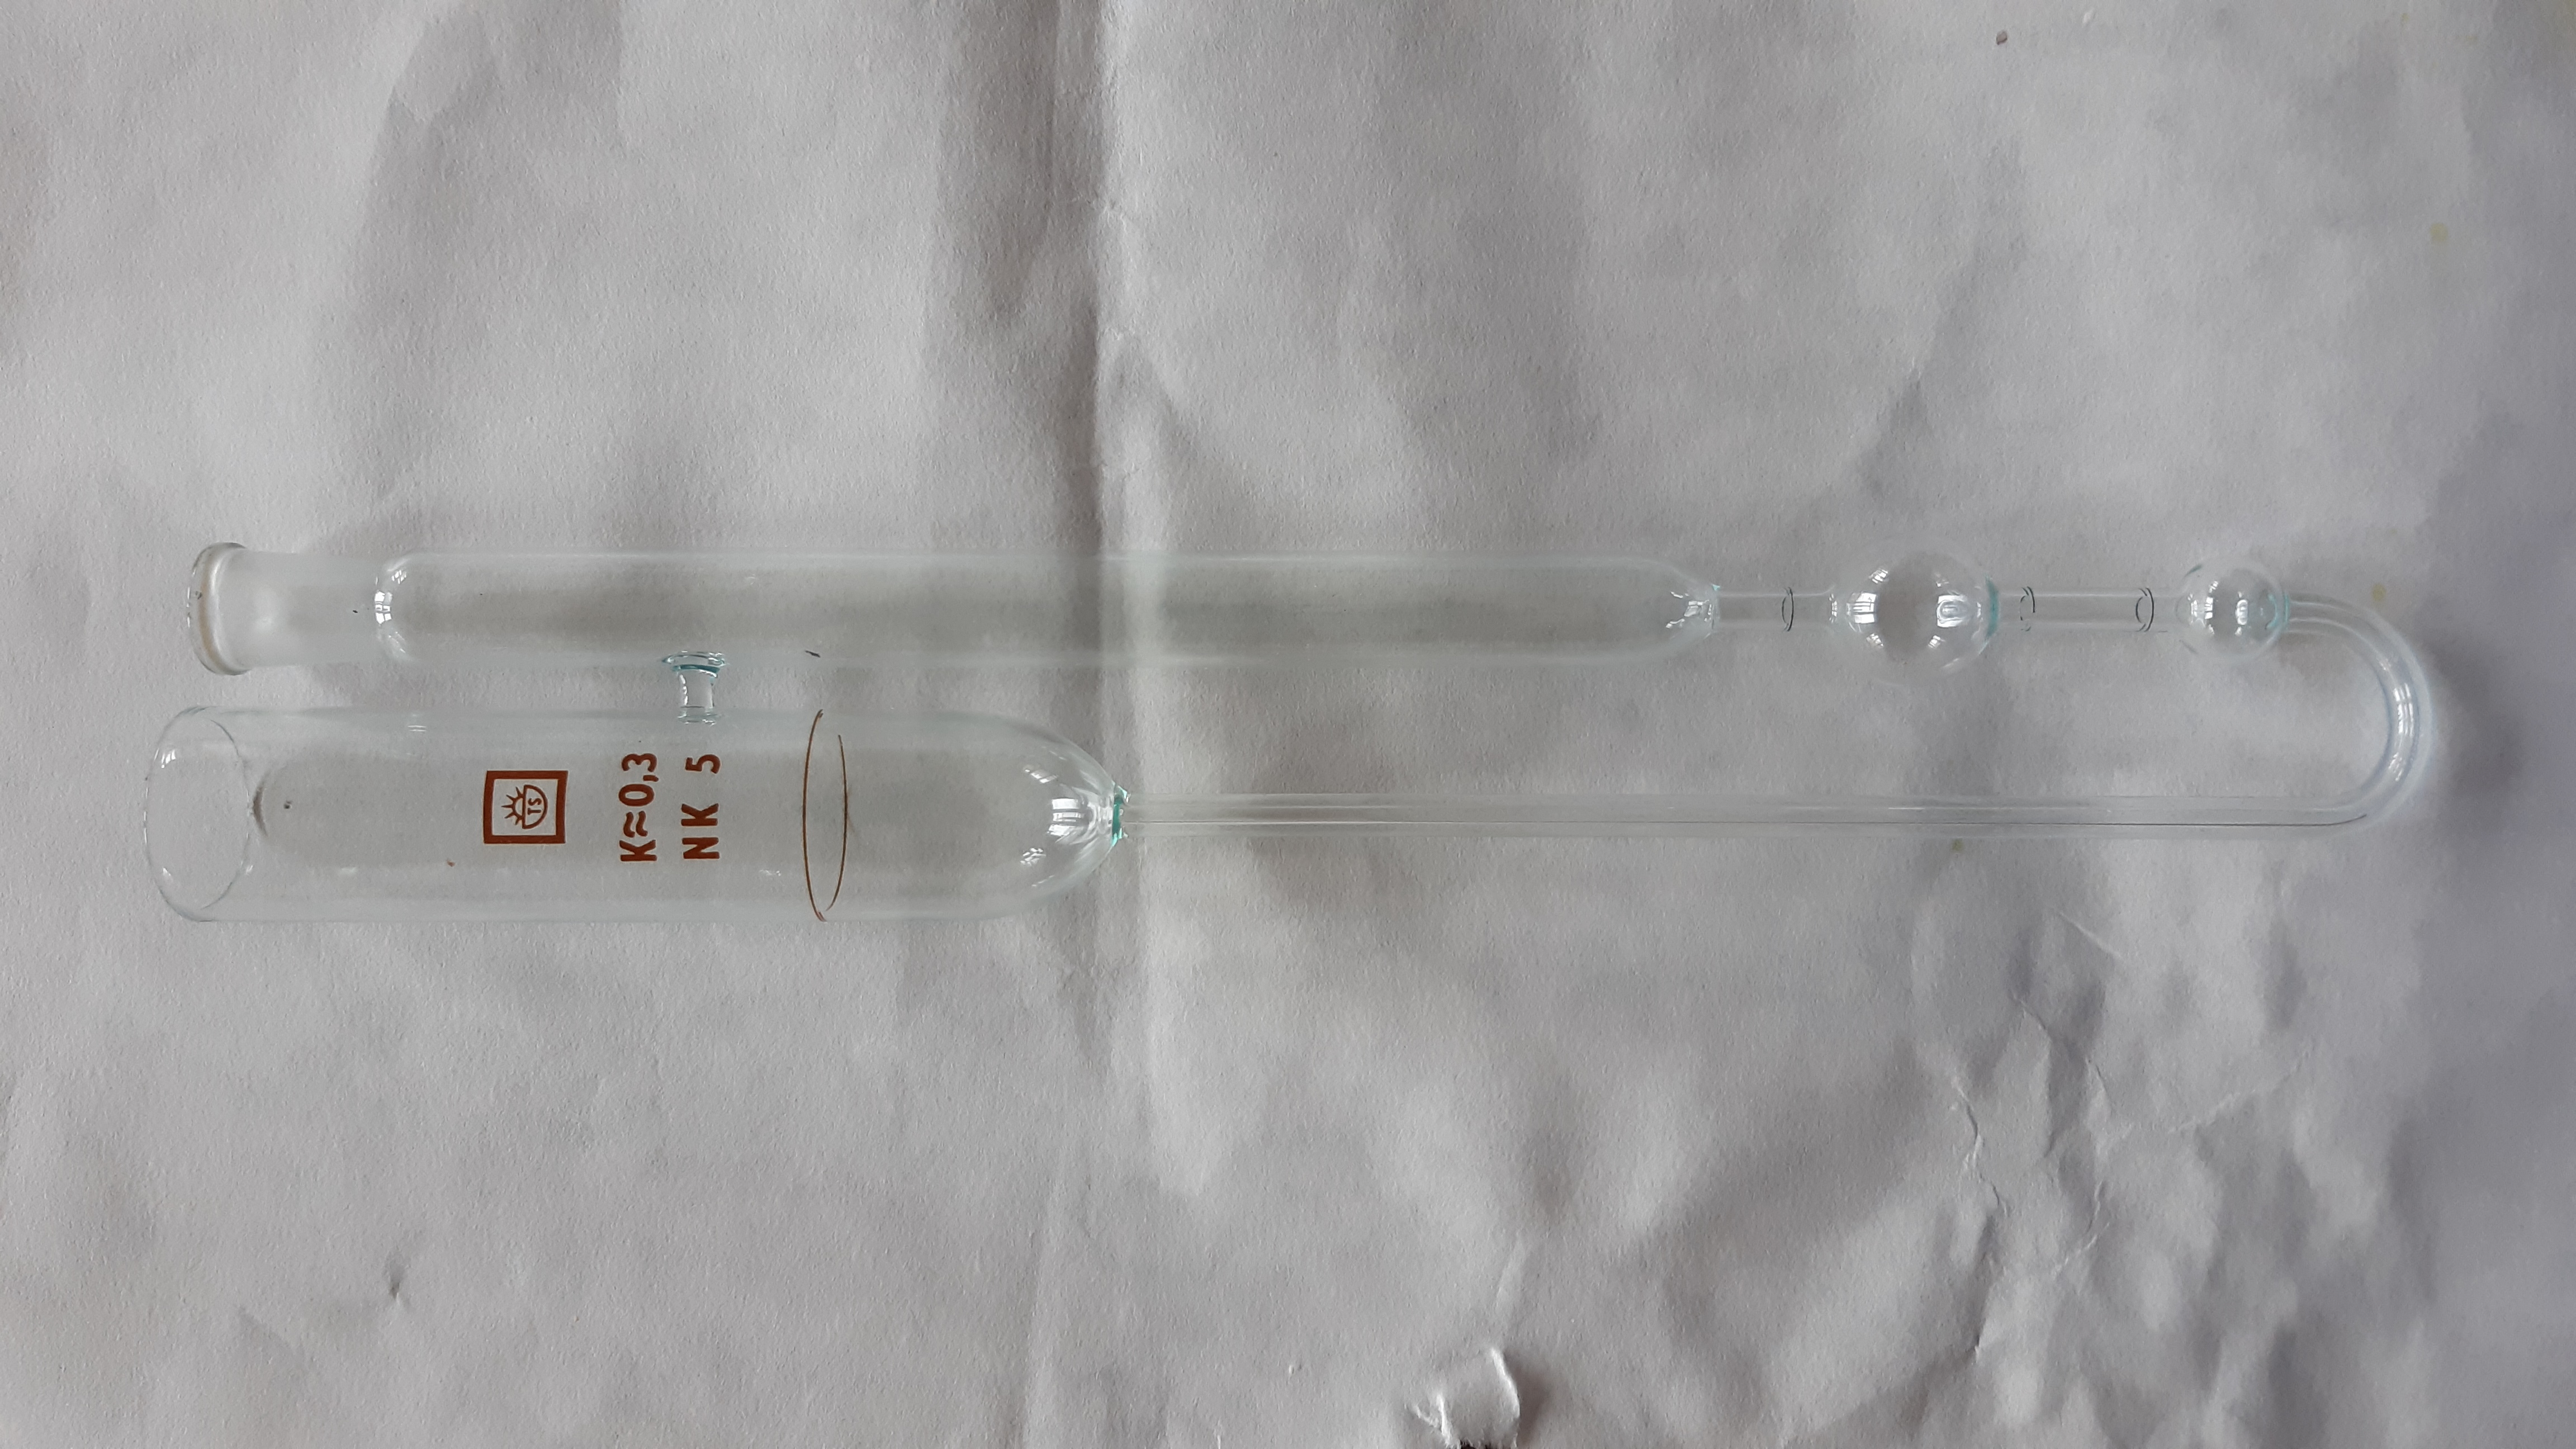
\includegraphics[angle = 270, width = \textwidth]{prilohy/muj_ostwald1.jpg}
    \end{subfigure}
    \hfill
    \begin{subfigure}[b]{.5\textwidth}
        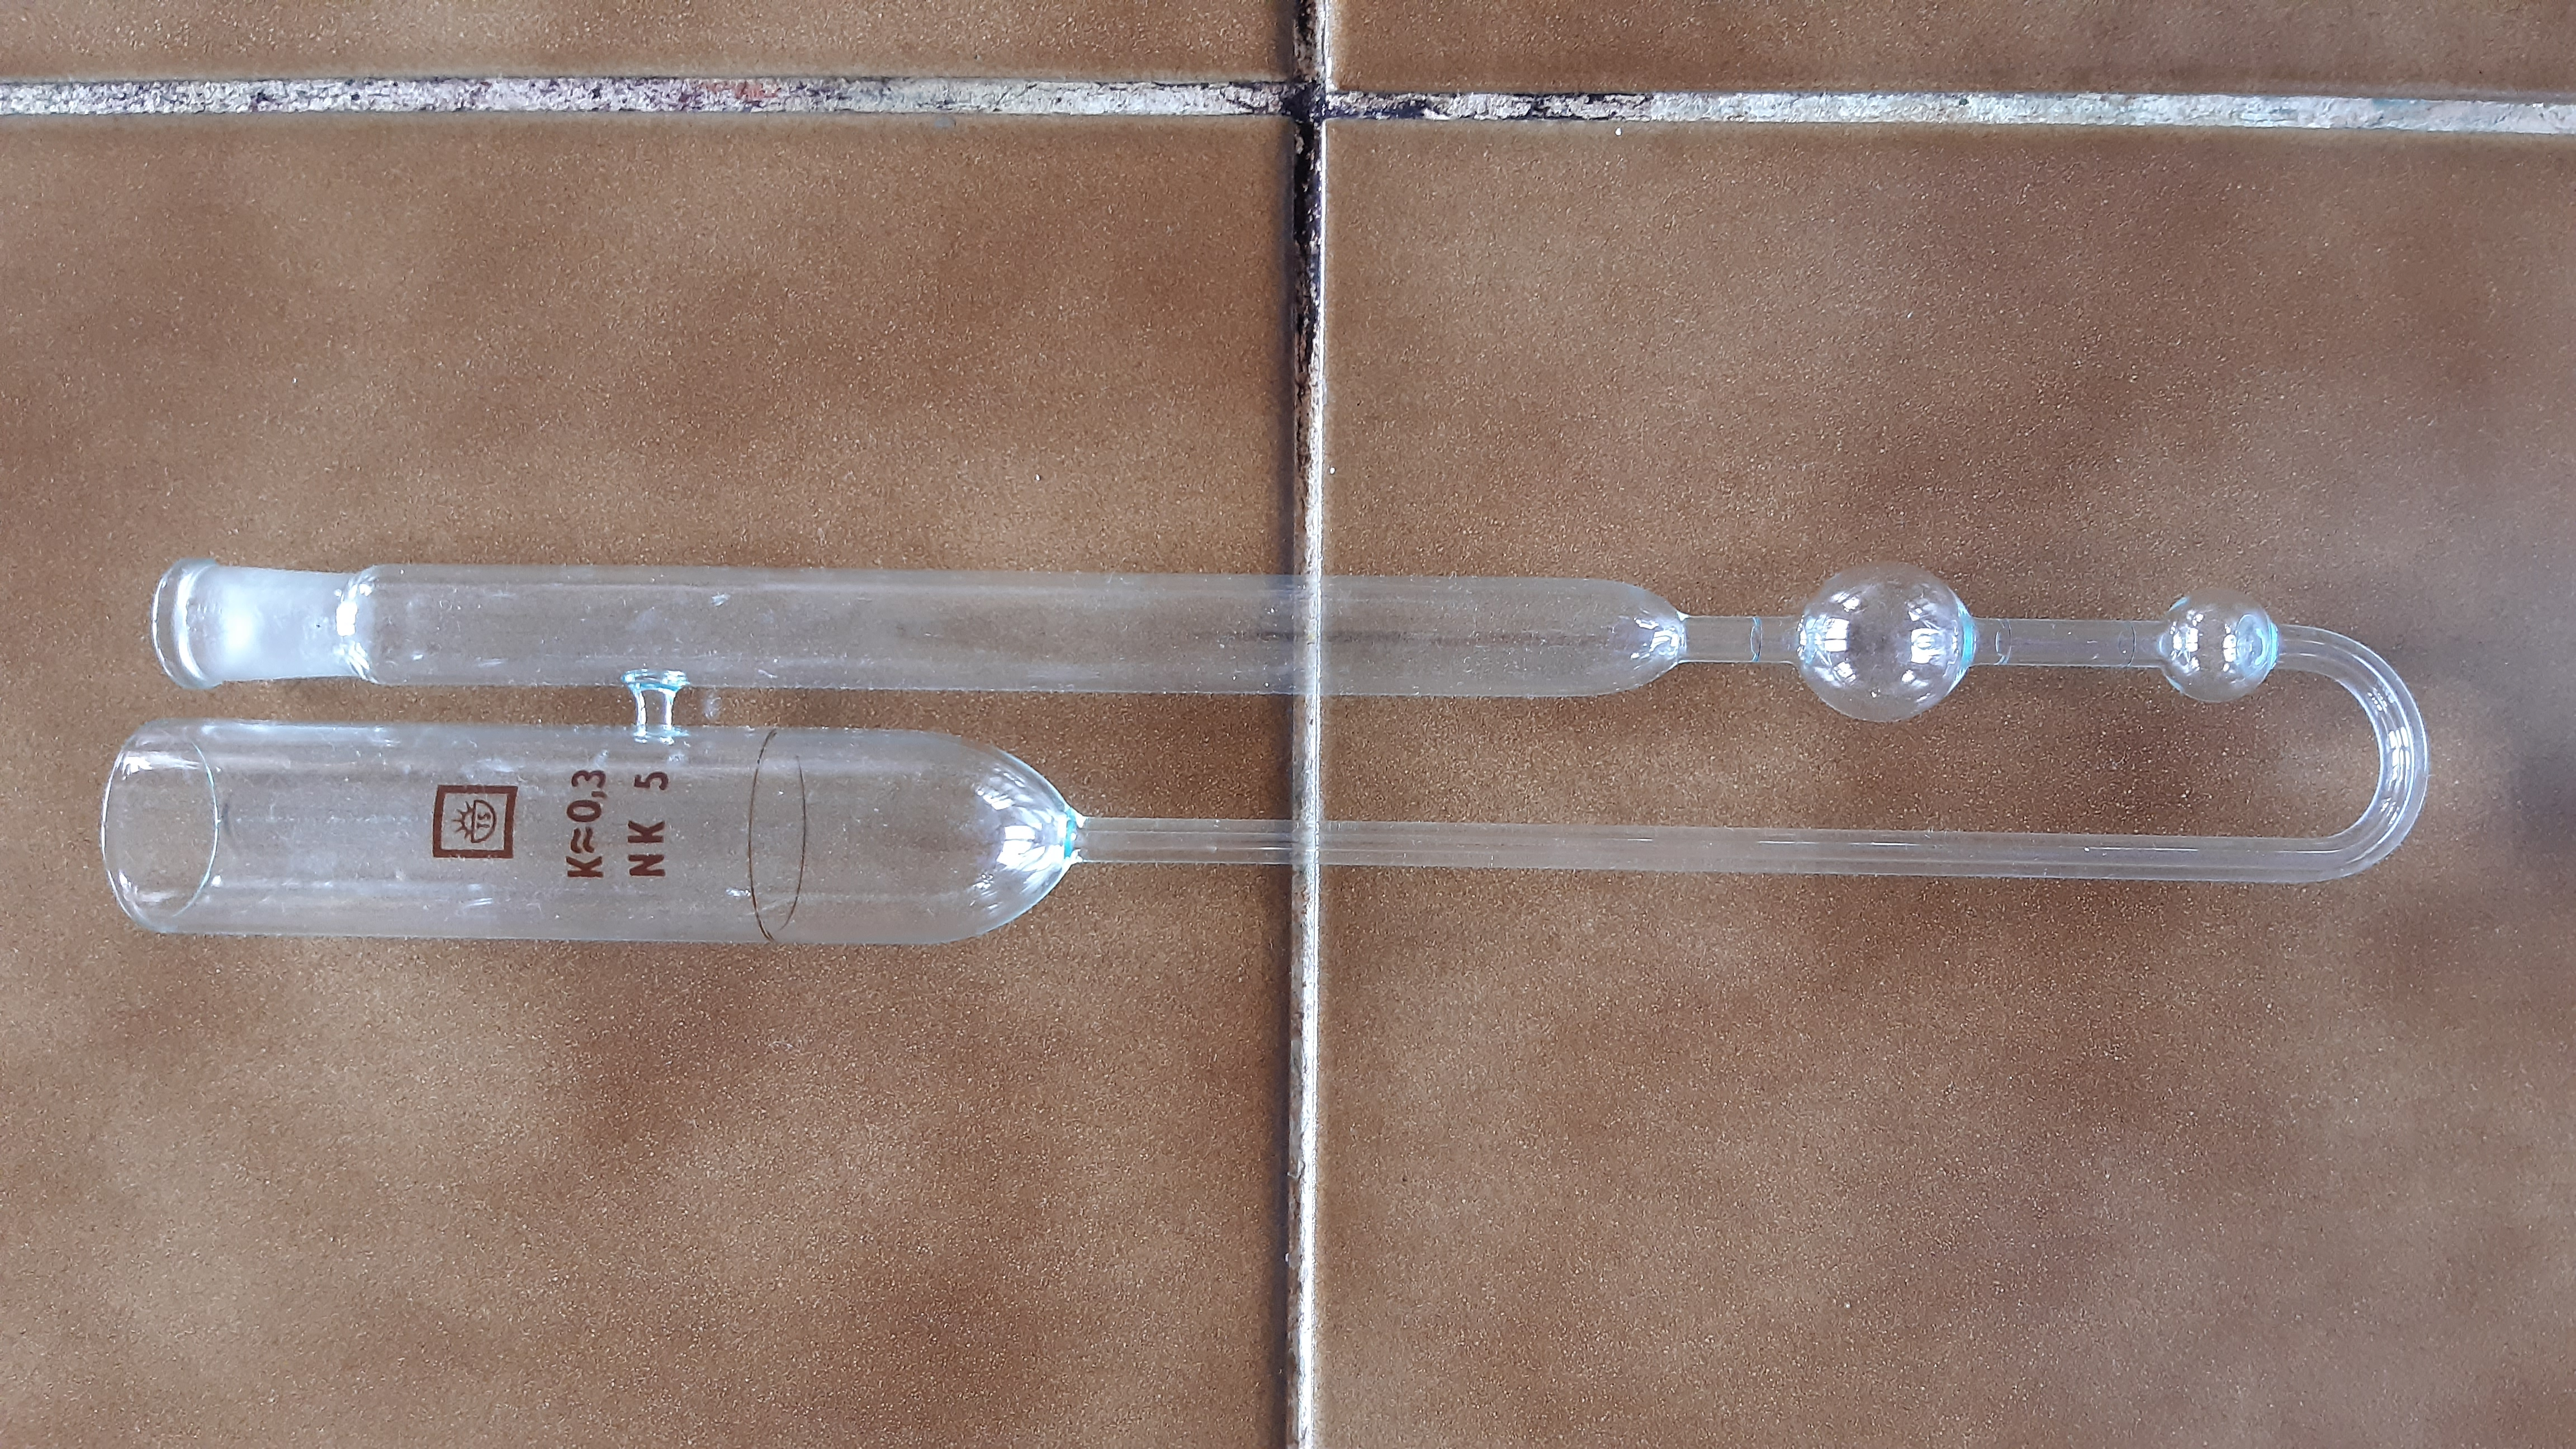
\includegraphics[angle = 270, width = \textwidth]{prilohy/muj_ostwald2.jpg}
    \end{subfigure}
    \caption{Použitý viskozimetr dle Ostwalda, jednou vyfocený na světlém a~podruhé na tmavém pozadí. Konstanta viskozimetru $k = 0,3$. Za povšimnutí stojí plnicí a~měřicí rysky.}
    \label{fig:muj_ostwald}
\end{figure}

\begin{figure}
    \centering
    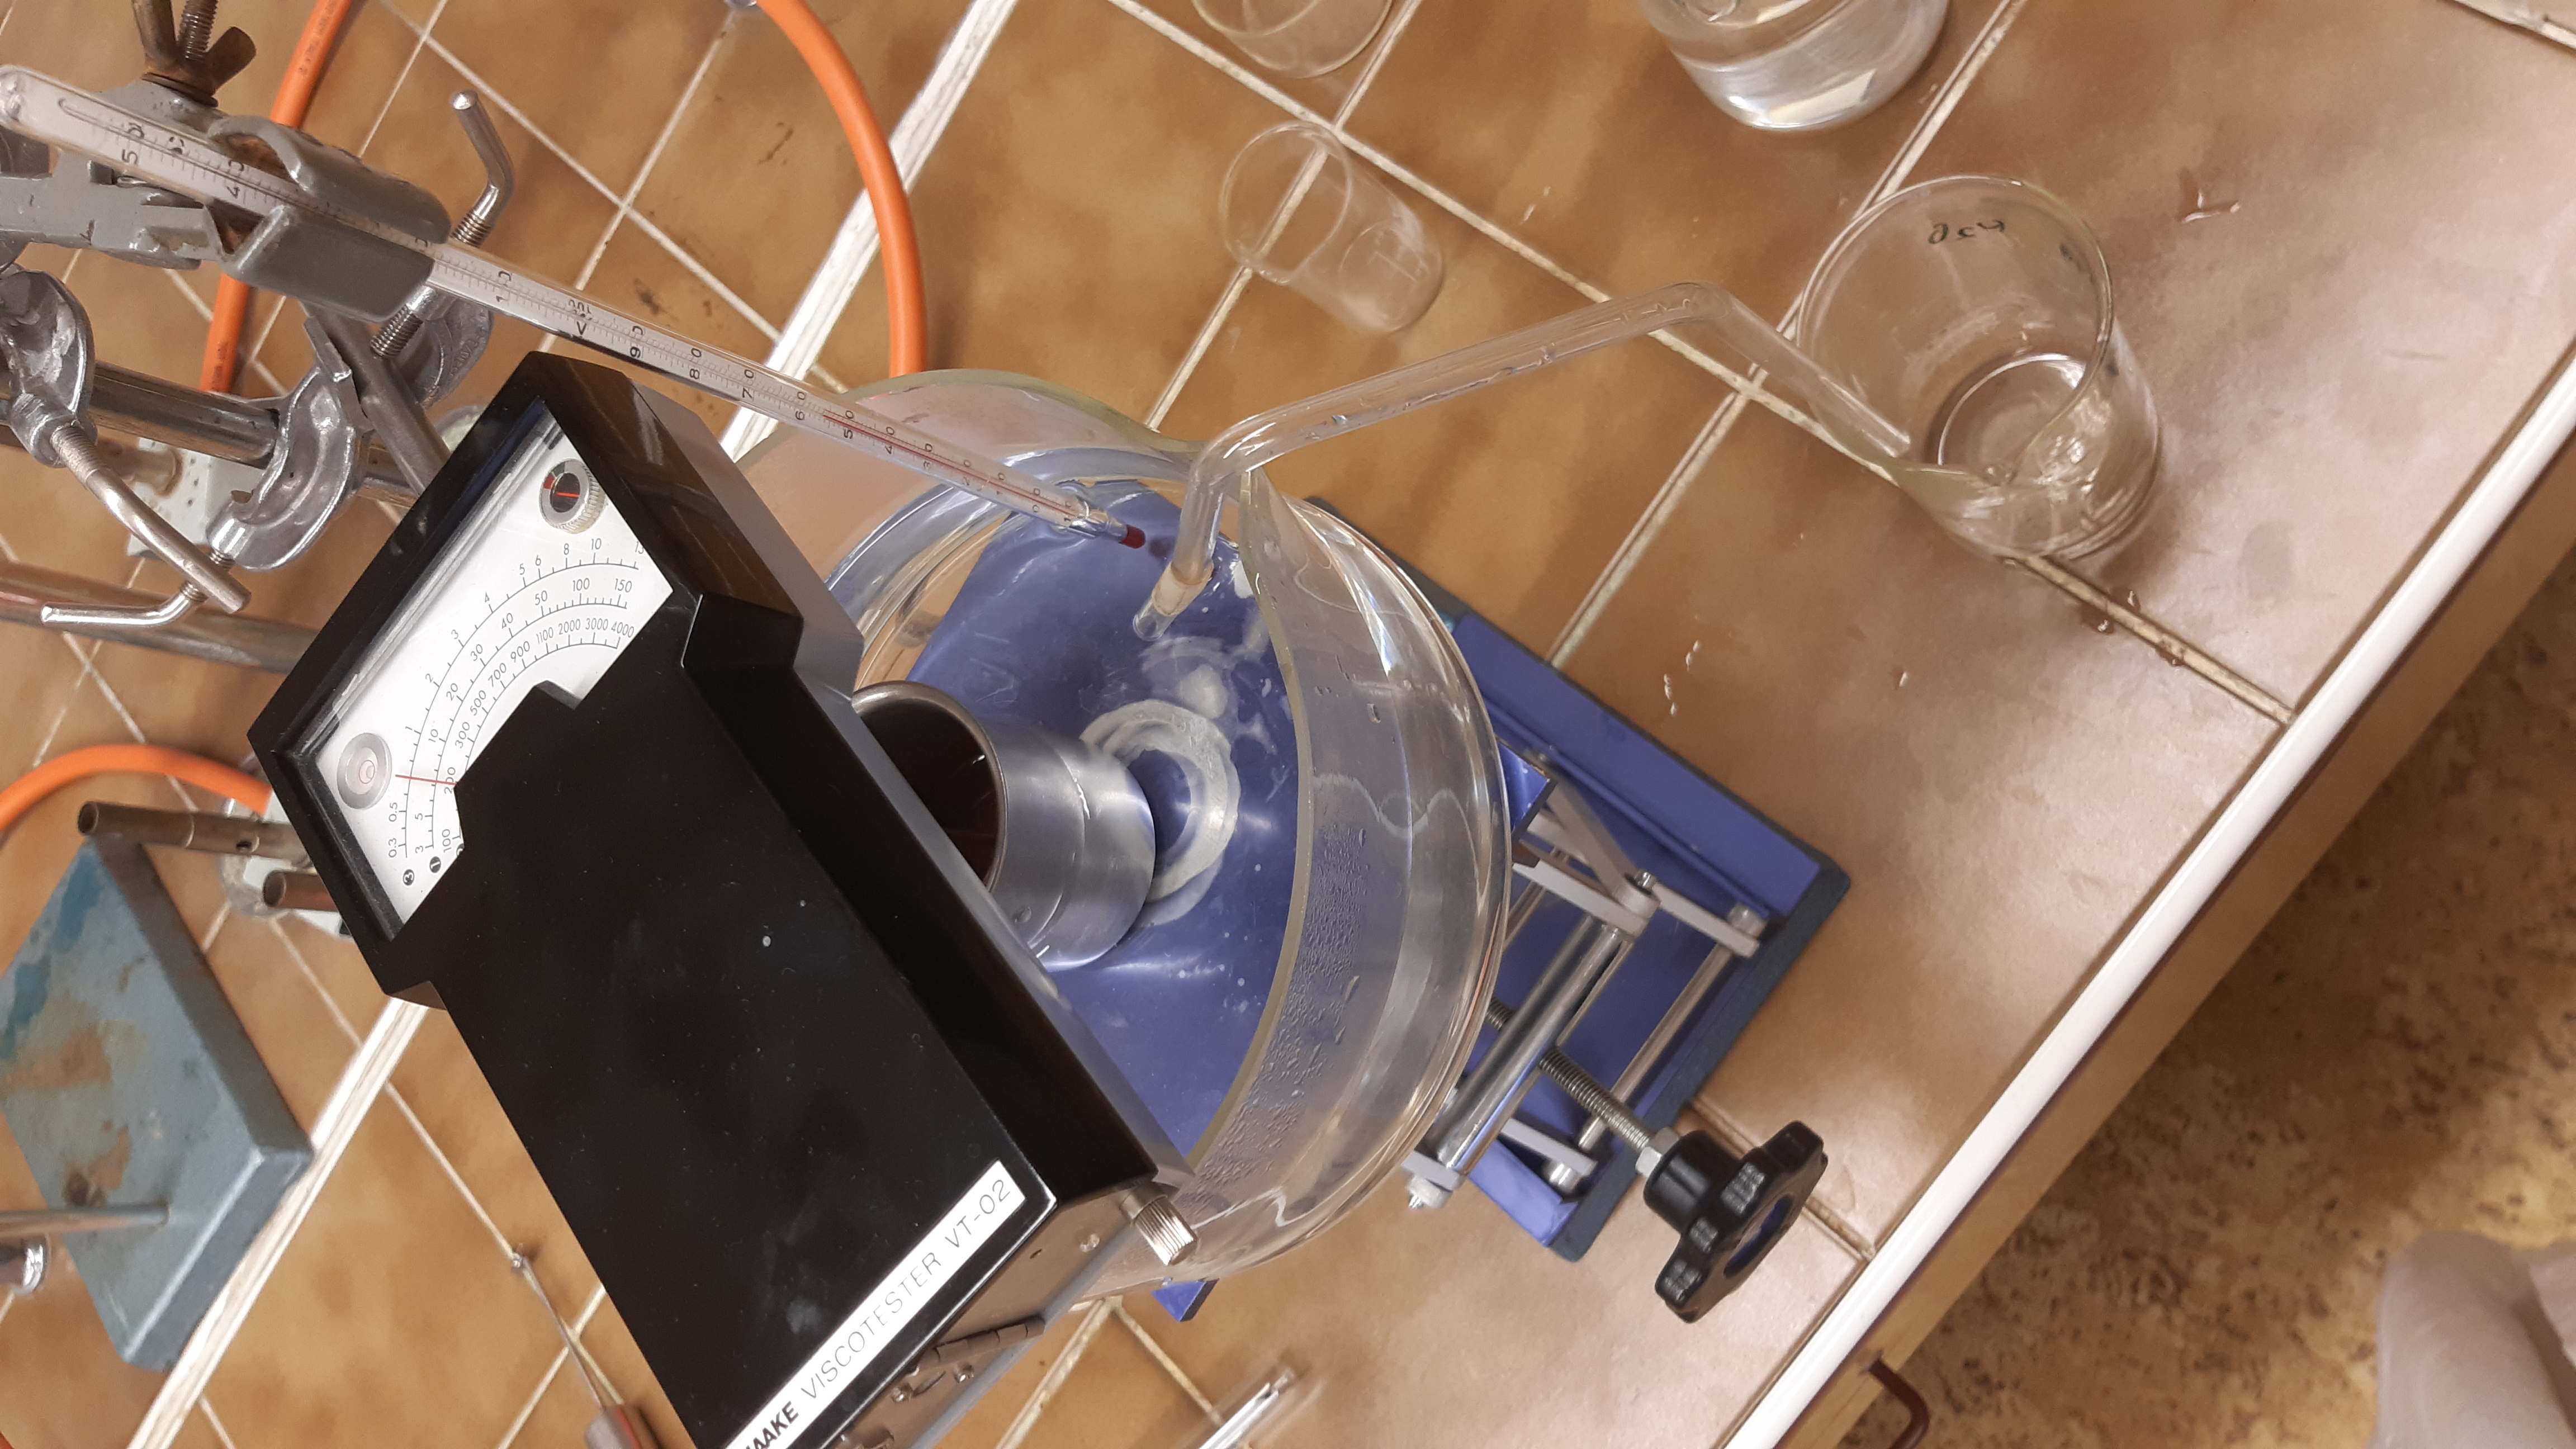
\includegraphics[angle = 270, width = 0.75\textwidth]{prilohy/aparatura_lab_vrch.jpg}
    \caption{Pohled na první implementaci aparatury z~vrchu. V~lázni je umístěna kovová kádinka s~čokoládovou taveninou. Do ní je ponořeno měřicí vřeteno viskozimetru. Miska lázně je umístěna na laboratorním zvedáčku a~teplota vody v~ní je měřena teploměrem. Z~lázně vede trubička určená k~odčerpání přebytečné vody z~lázně.}
    \label{fig:aparatura_lab_bok}
\end{figure}

\begin{figure}[h!]
    \begin{subfigure}[b]{\textwidth}
    \centering
        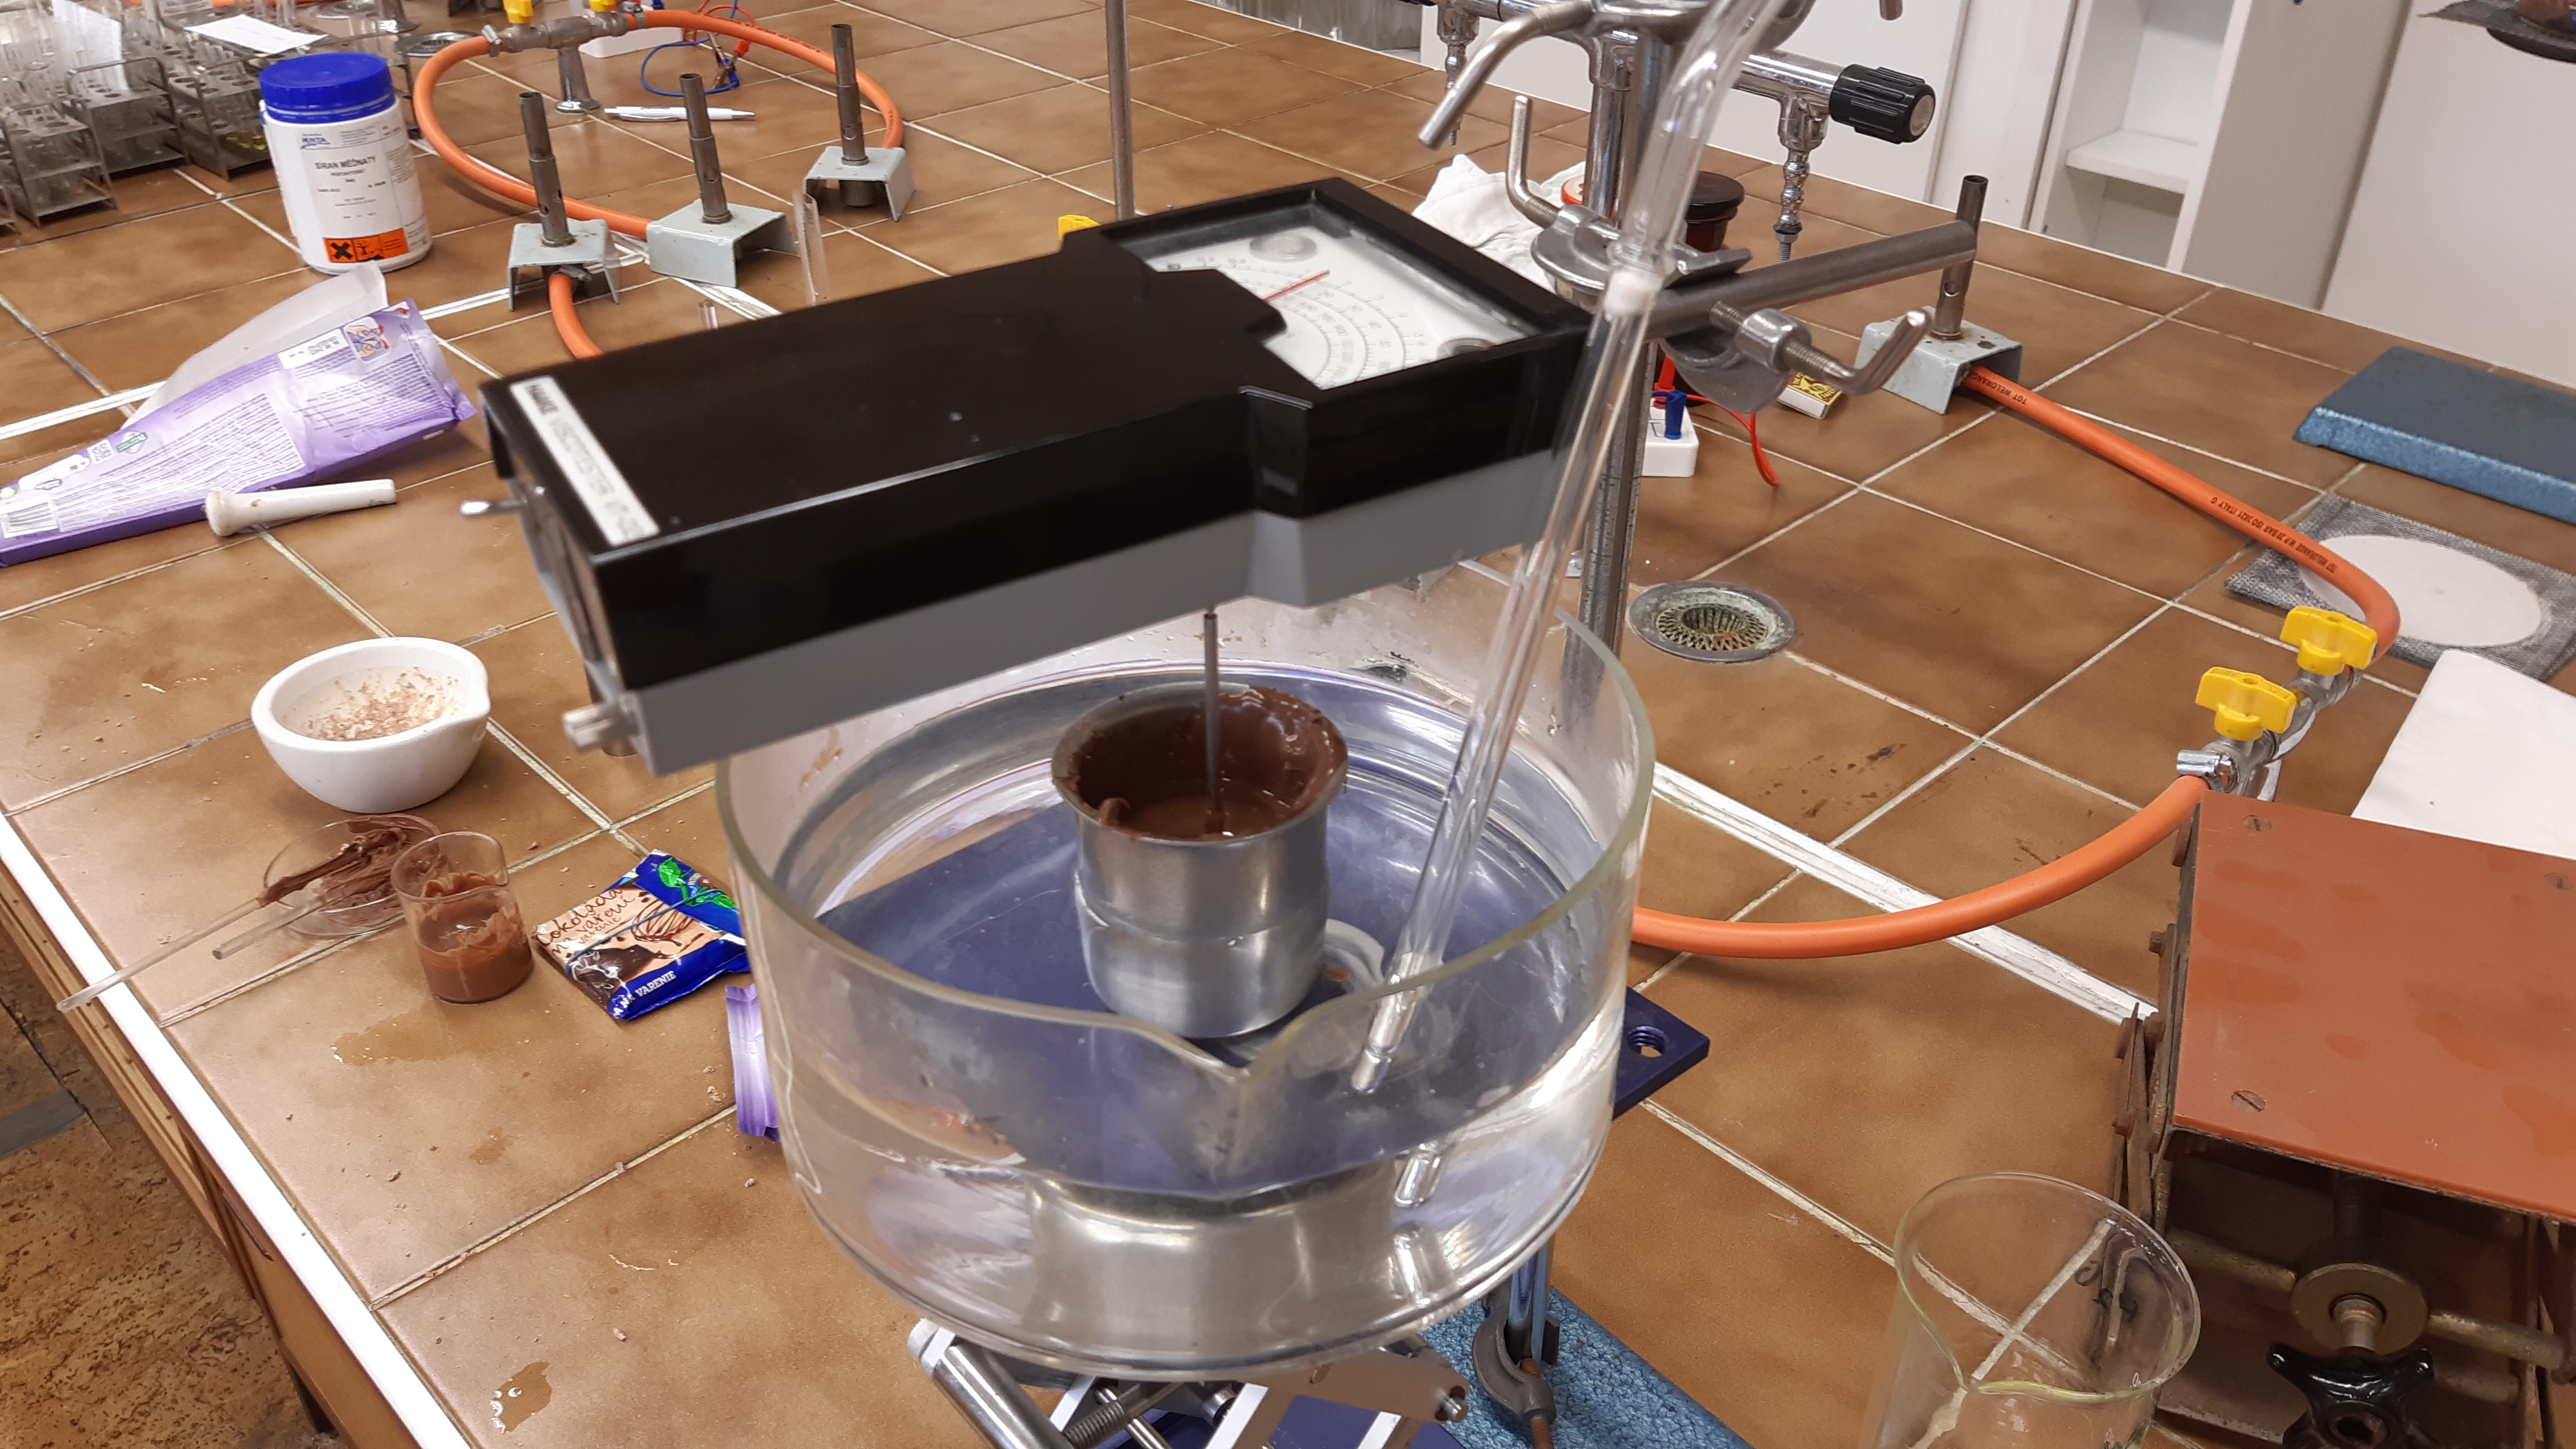
\includegraphics[width = \textwidth]{prilohy/aparatura_lab_bok.jpg}
    \end{subfigure}
    \hfill
    \begin{subfigure}[b]{\textwidth}
        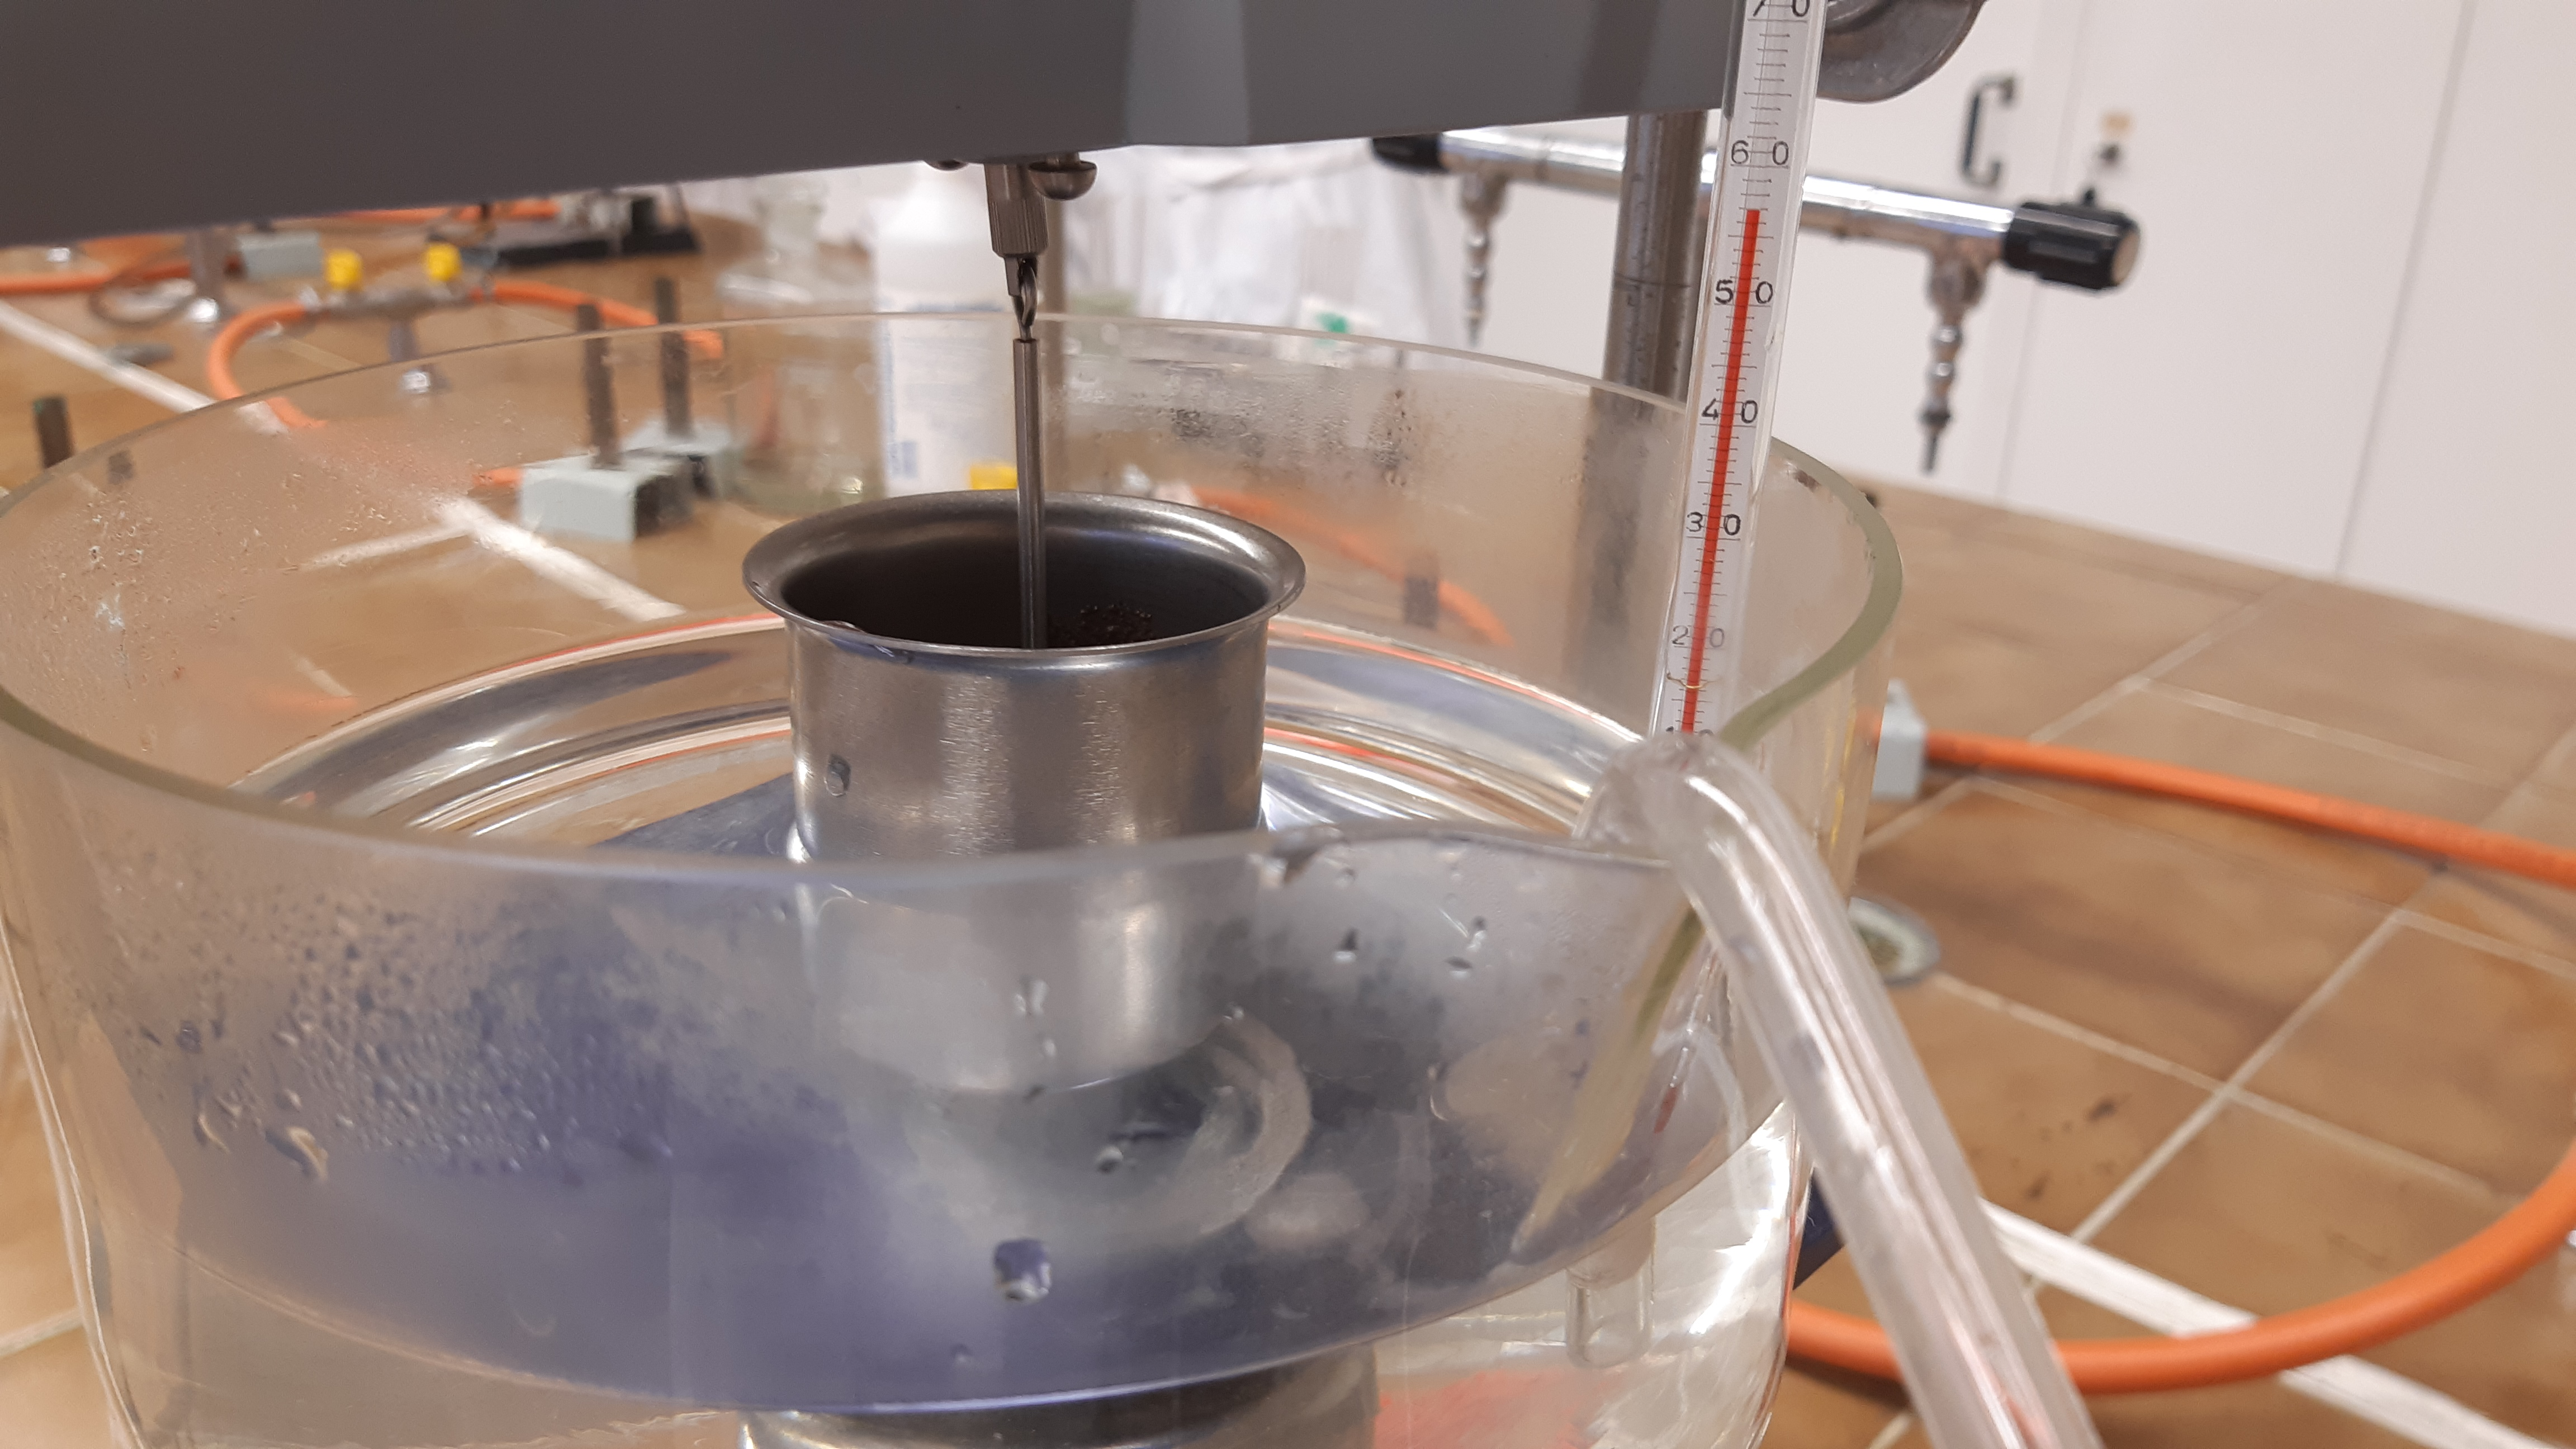
\includegraphics[width = \textwidth]{prilohy/lab_lázeň.jpg}
    \end{subfigure}
    \caption{Pohled na první implementaci aparatury z~boku (nahoře) a~detailní záběr lázně (dole). V~lázni je umístěna kovová kádinka s~čokoládovou taveninou. Do ní je ponořeno měřicí vřeteno viskozimetru. Miska lázně je umístěna na laboratorním zvedáčku a~teplota vody v~ní je měřena teploměrem. Na spodním obrázku je vidět trubička, která je určena k~odčerpávání přebytečné vody z~lázně.}
    \label{fig:aparatura_lab}
\end{figure}

\begin{figure}
    \begin{subfigure}[t]{\textwidth}
        \centering
        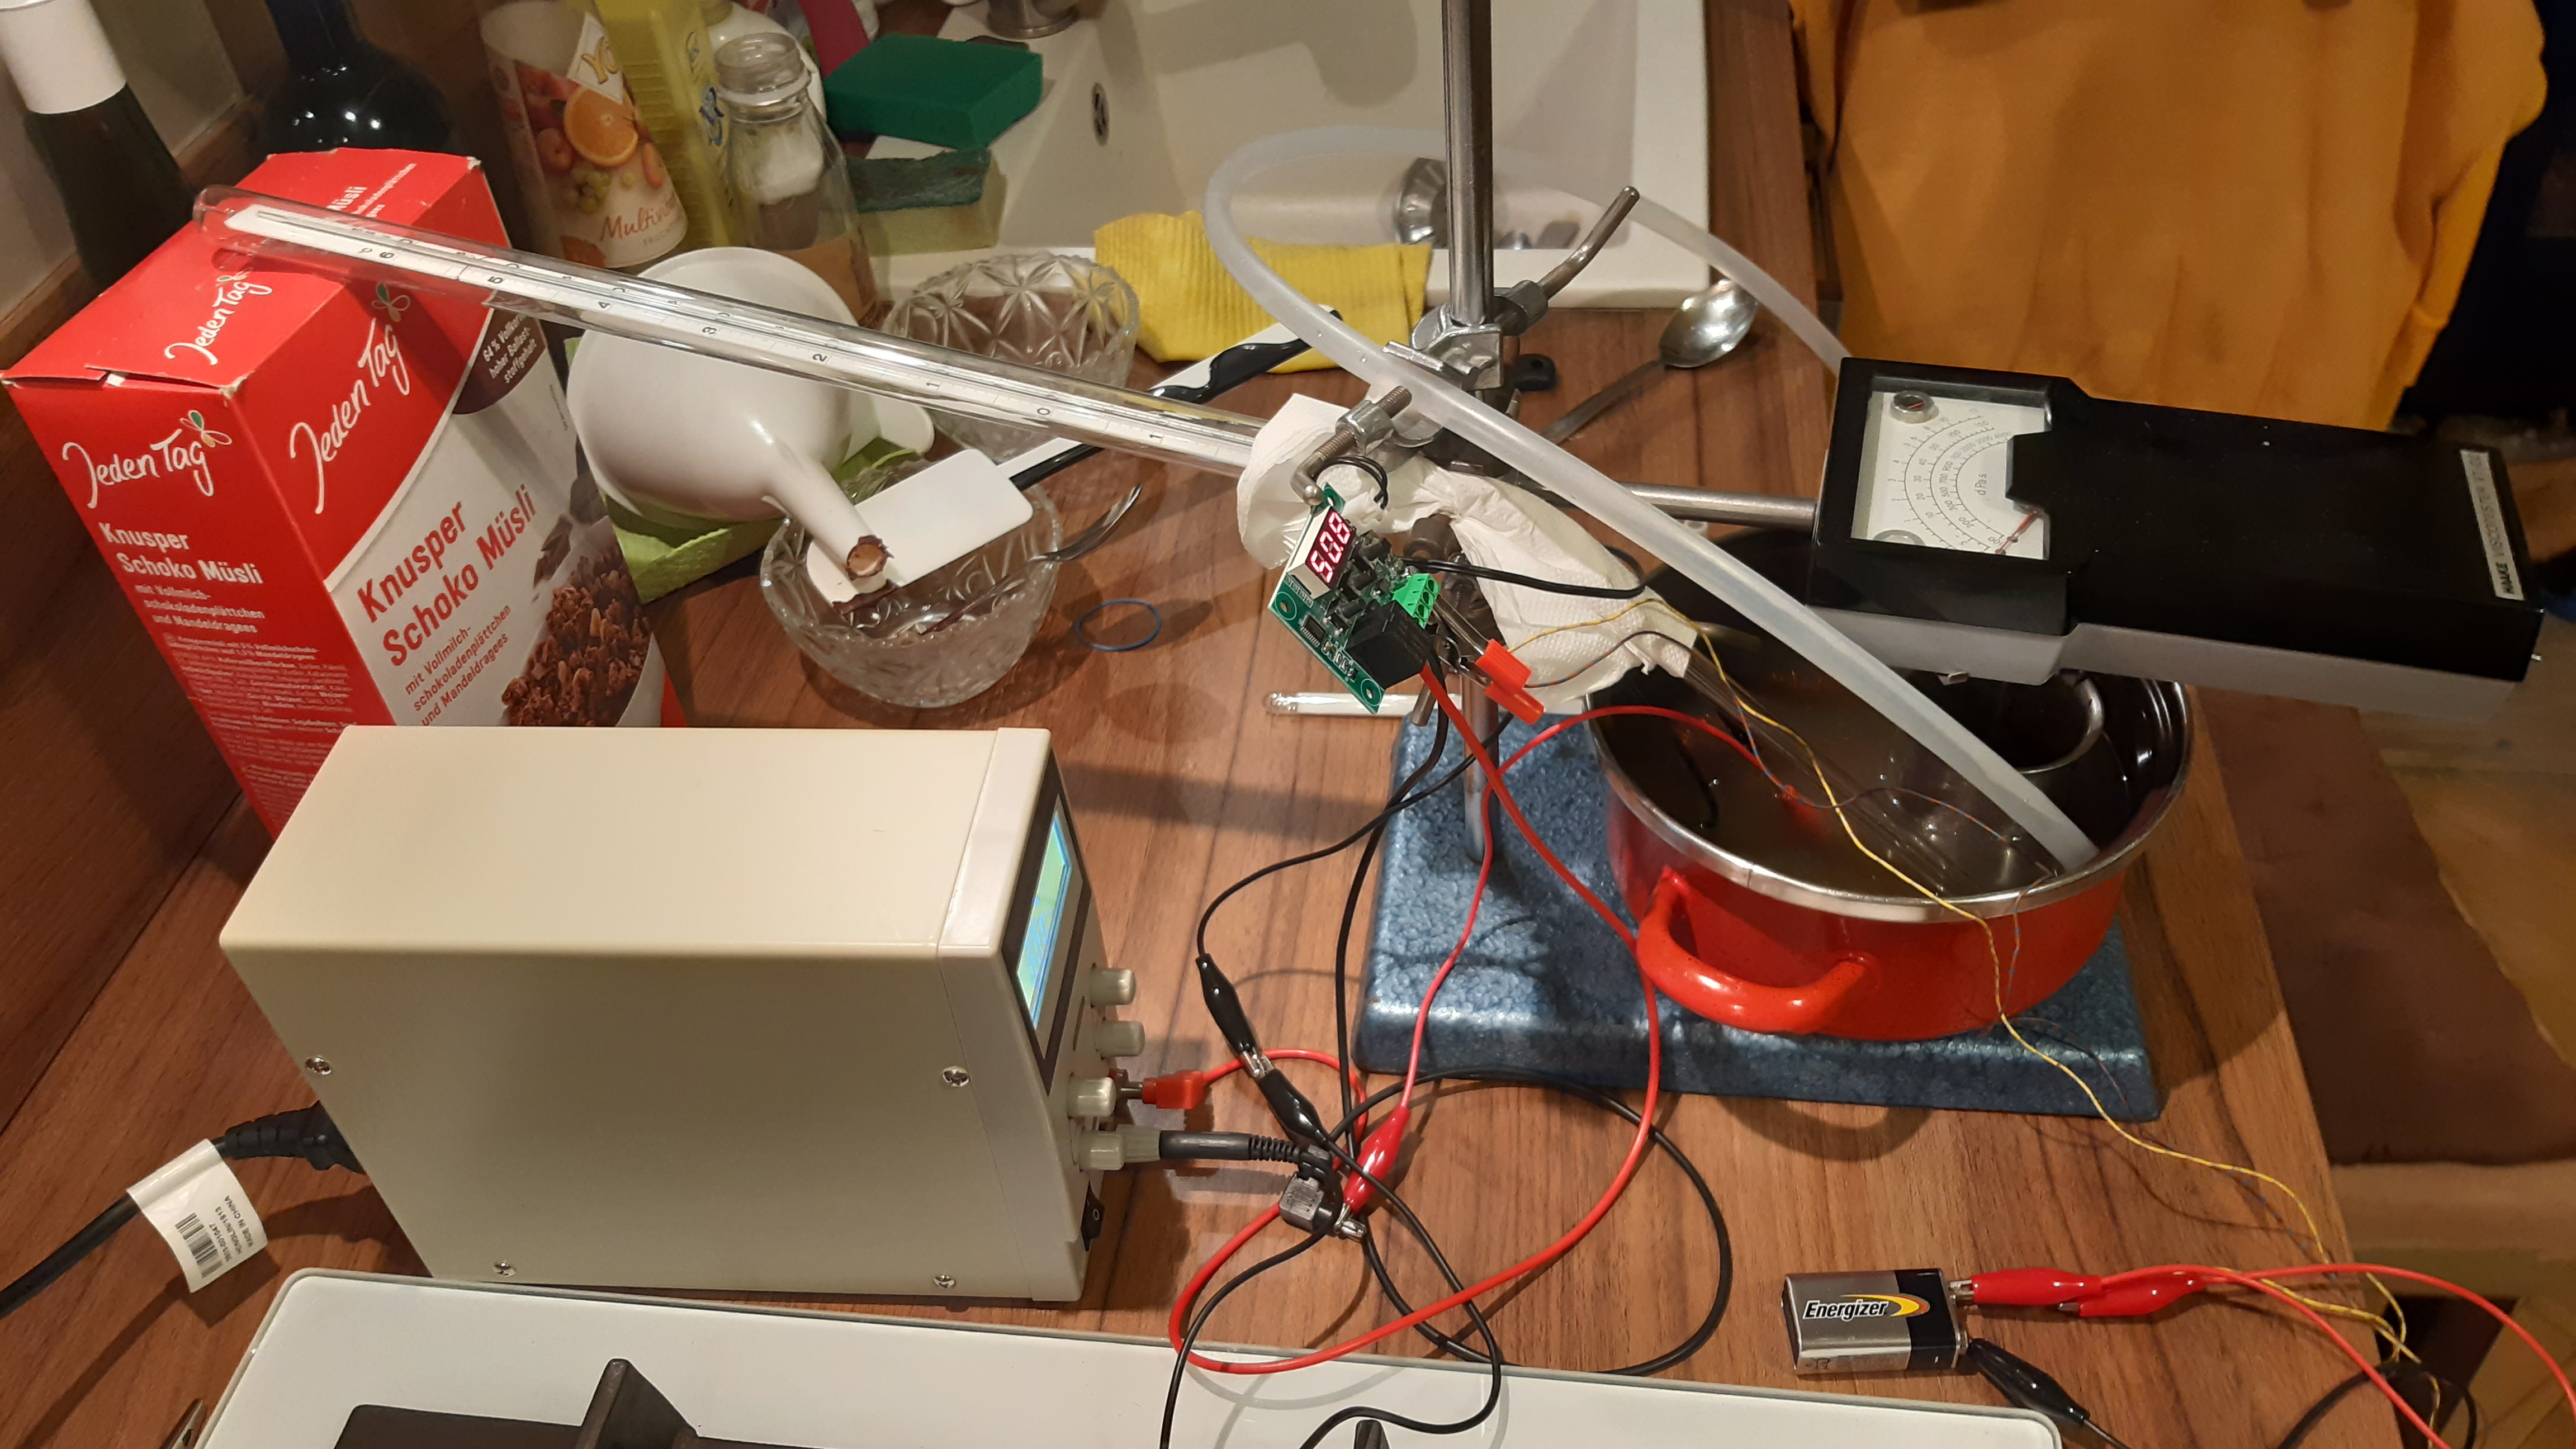
\includegraphics[width = 0.95\textwidth]{prilohy/aparatura_bok.jpg}
        \caption{Pohled na druhou implementaci aparatury z~boku. Červený hrnec tvoří vodní lázeň. V~něm je umístěna kovová kádinka s~čokoládovou taveninou, do které je umístěno měřicí vřeteno viskozimetru. Z~lázně obloukem vede plastová hadice určená k~odčerpávání přebytečné vody z~lázně. V~lázni je zároveň umístěn stonek rtuťového teploměru, který se opírá o~krabici Schoko Müsli. \SI{9}{\volt} baterie v~pravé spodní části obrázku napájí modul termostatu (zhruba uprostřed obrázku). Termostat indikuje teplotu lázně \SI{50,8}{\degreeCelsius}. V~lázni je umístěna cívka smotaná z~měděného drátu (na obrázku není vidět), která slouží jako topné těleso. Dobře je vidět do hrnce ponořený červený vodič, který cívku napájí. Topné těleso je napájeno pomocí laboratorního zdroje stejnosměrného napětí (levá dolní část obrázku).}
        \label{fig:aparatura_bok}
    \end{subfigure}
    \hfill
    \begin{subfigure}[t]{\textwidth}
        \centering
        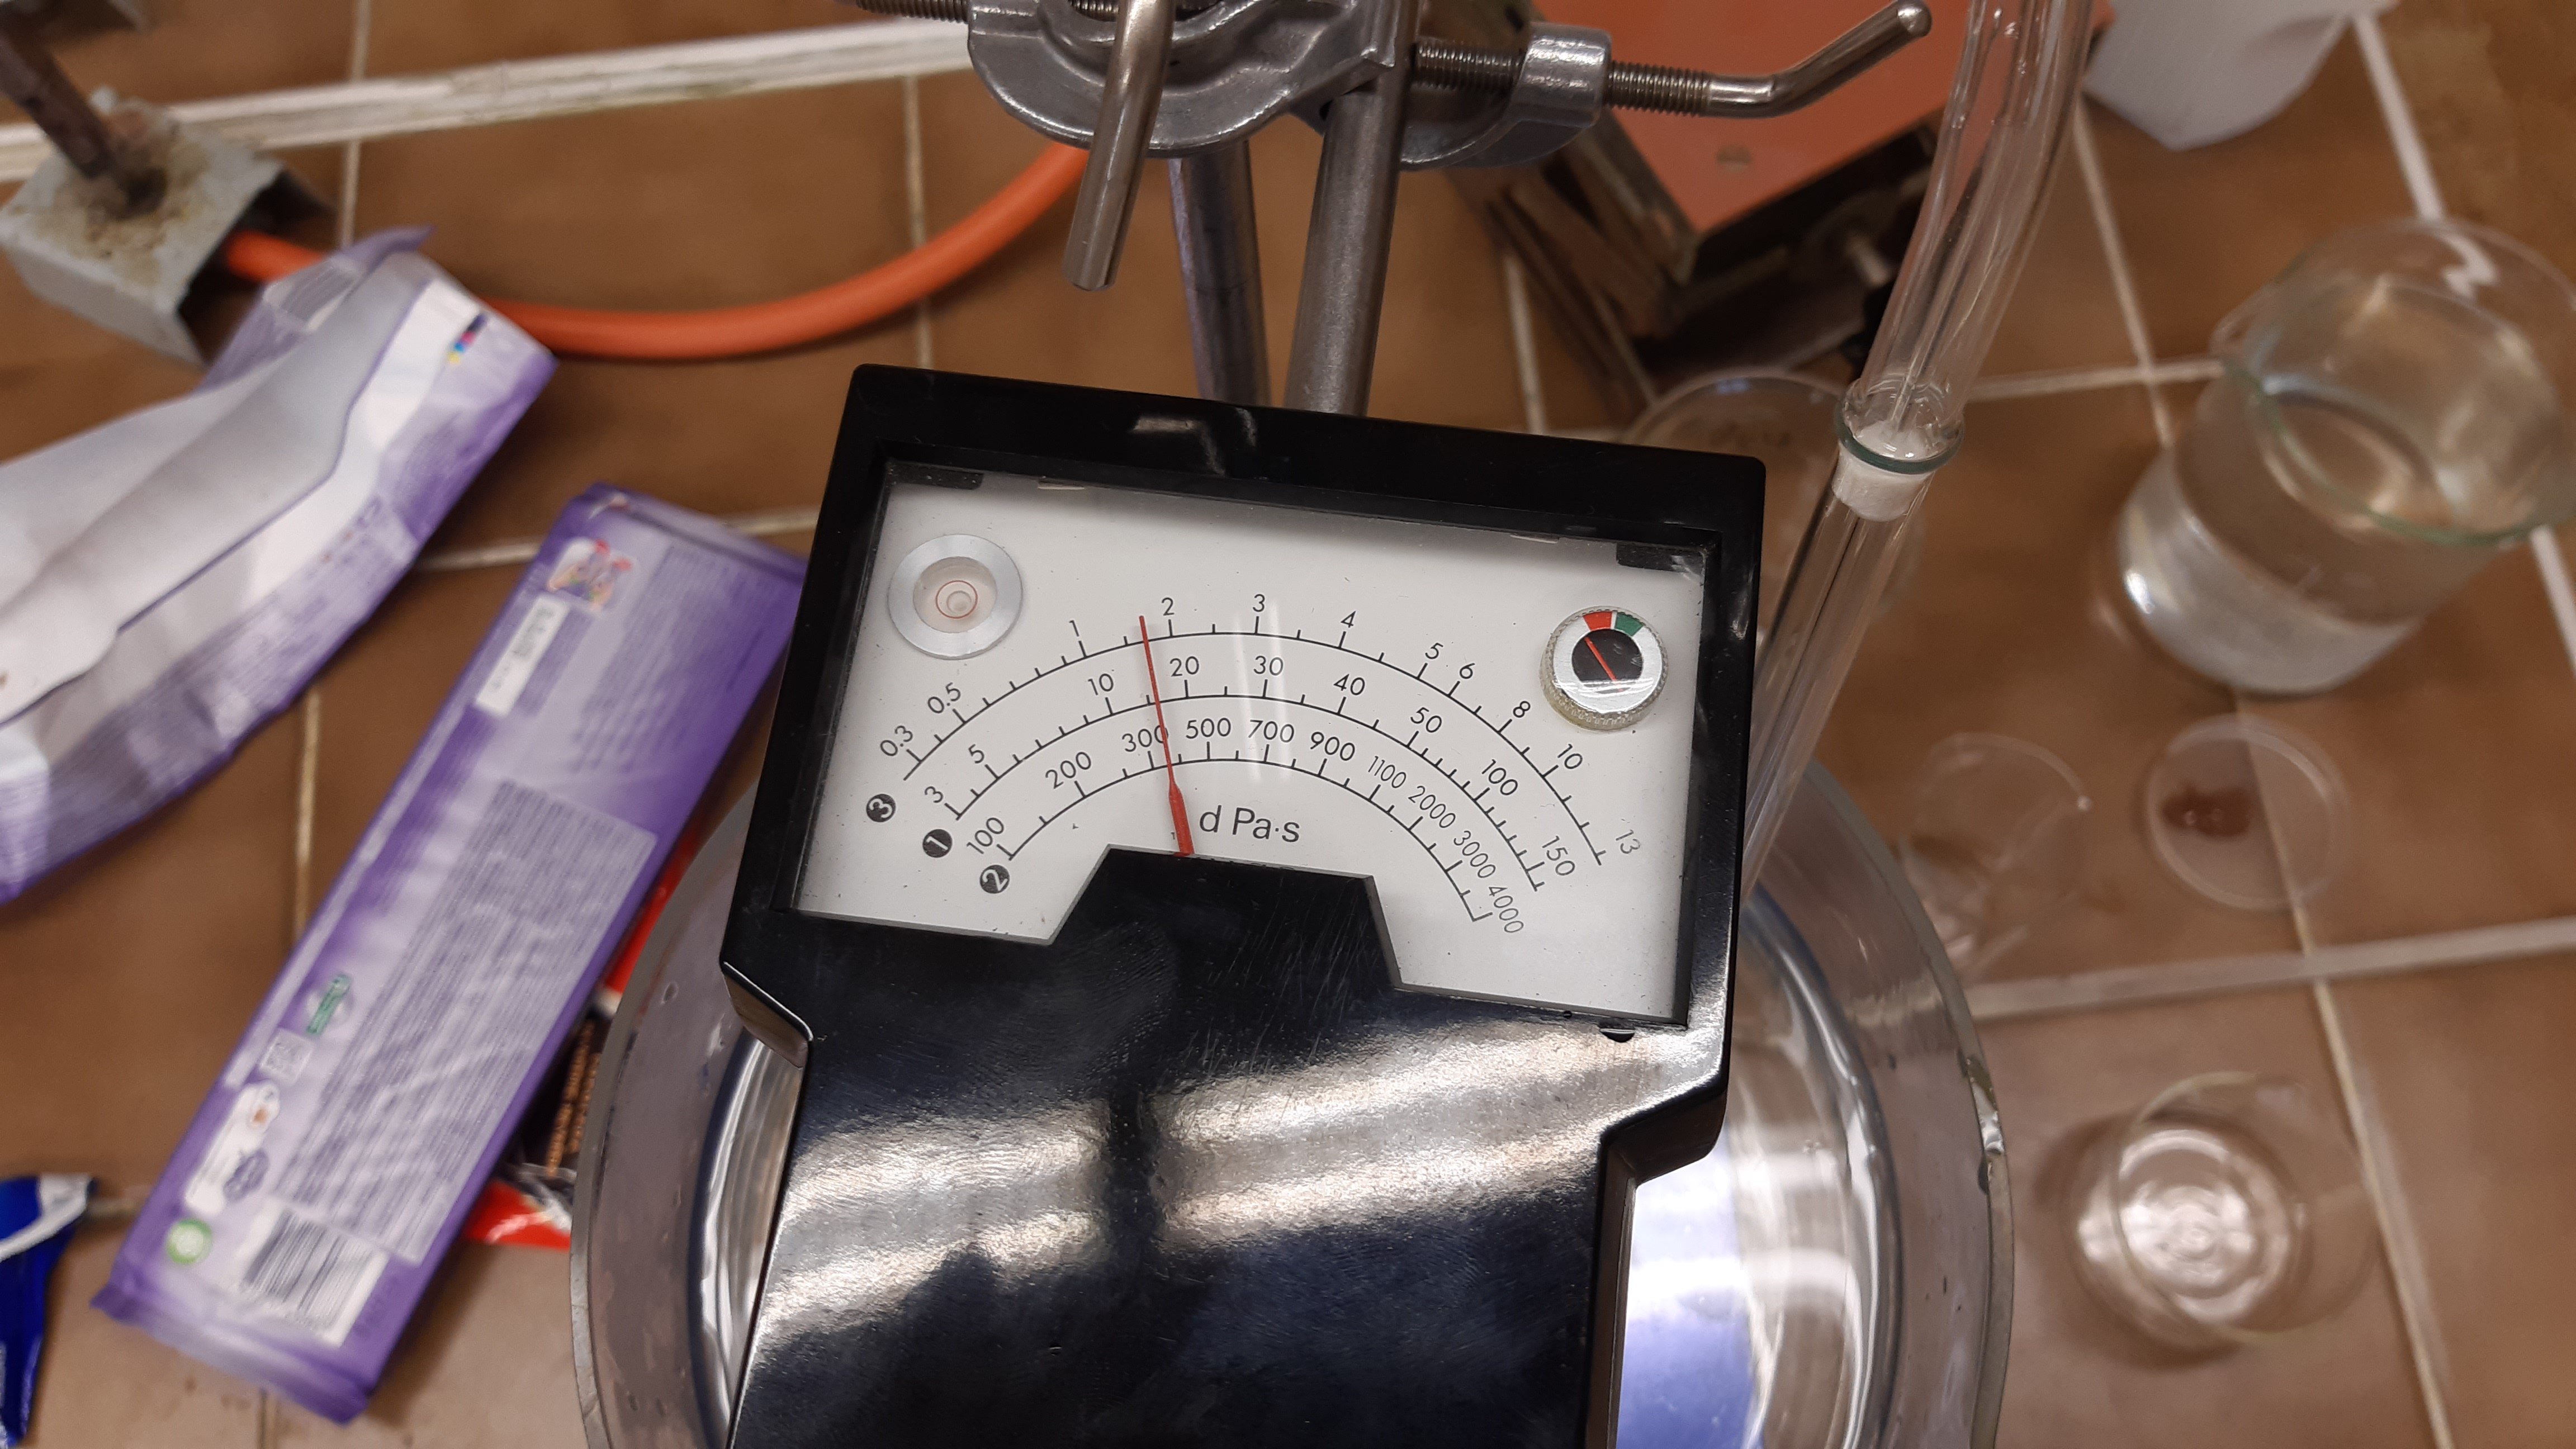
\includegraphics[width = 0.95\textwidth]{prilohy/viskozimetr_1.jpg}
        \caption{Detail indikační části použitého viskozimetru. Při použitém měřicím vřetenu č.~2 je naměřená hodnota zdánlivé viskozity zhruba \SI{360}{\deci\pascal\second}.}
    \end{subfigure}
    \caption{Pohled na druhou implementaci aparatury z~boku (nahoře) a~detail použitého rotačního viskozimetru (dole).}
\end{figure}

\begin{figure}[h!]
    \begin{subfigure}[t]{.45\textwidth}
        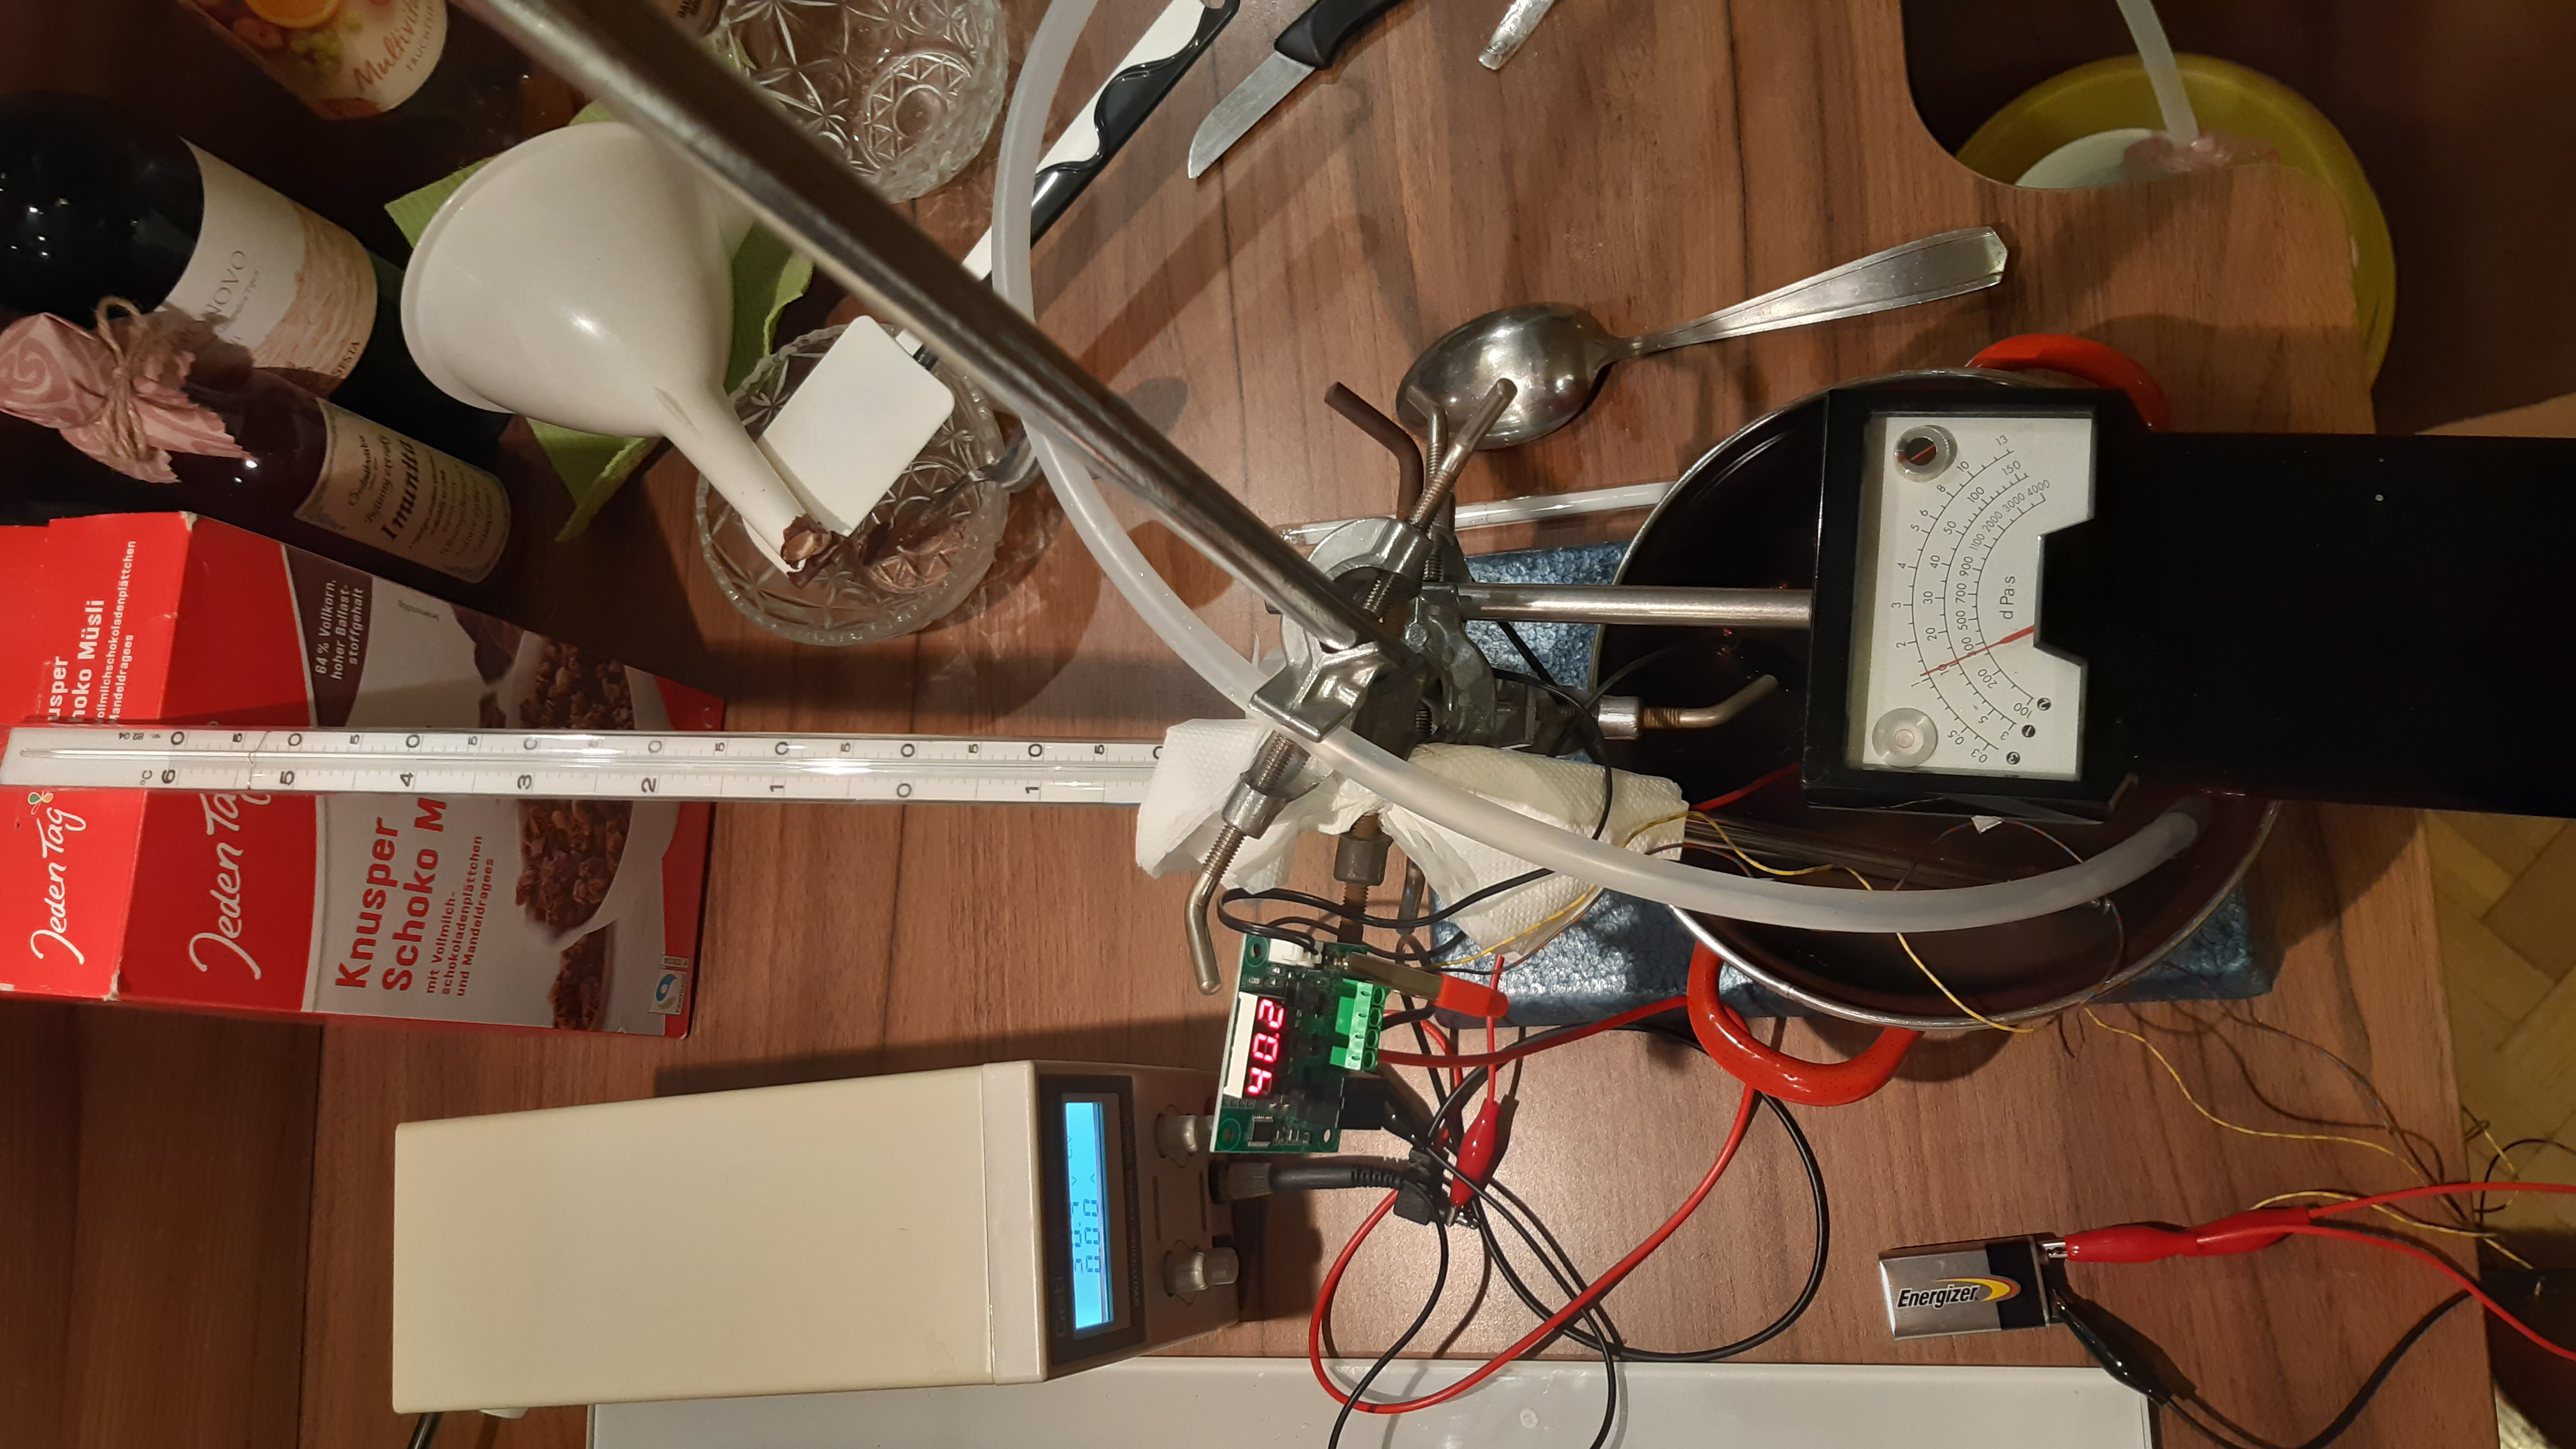
\includegraphics[angle = 270, width = \textwidth]{prilohy/aparatura_vrch.jpg}
        \caption{Pohled na druhou implementaci aparatury z~vrchu. Z~hrnce ve spodní části obrázku, který tvoří vodní lázeň, vede plastová hadička k~odčerpávání přebytečné vody z~lázně. Nad hrncem, resp.~kádinkou s~čokoládovou taveninou, je umístěn viskozimetr. Do vodní lázně je ponořen stonek rtuťového teploměru. V~levé části obrázku je vidět laboratorní zdroj, termostat indikující teplotu lázně \SI{40,2}{\degreeCelsius} a~\SI{9}{\volt} baterie napájející termostat. Indikační LED termostatu nesvítí, relé termostatu je tedy rozepnuté a~lázeň není vyhřívána (nastavená teplota byla \SI{40,0}{\degreeCelsius}).}
    \end{subfigure}
    \hfill
    \begin{subfigure}[t]{.45\textwidth}
        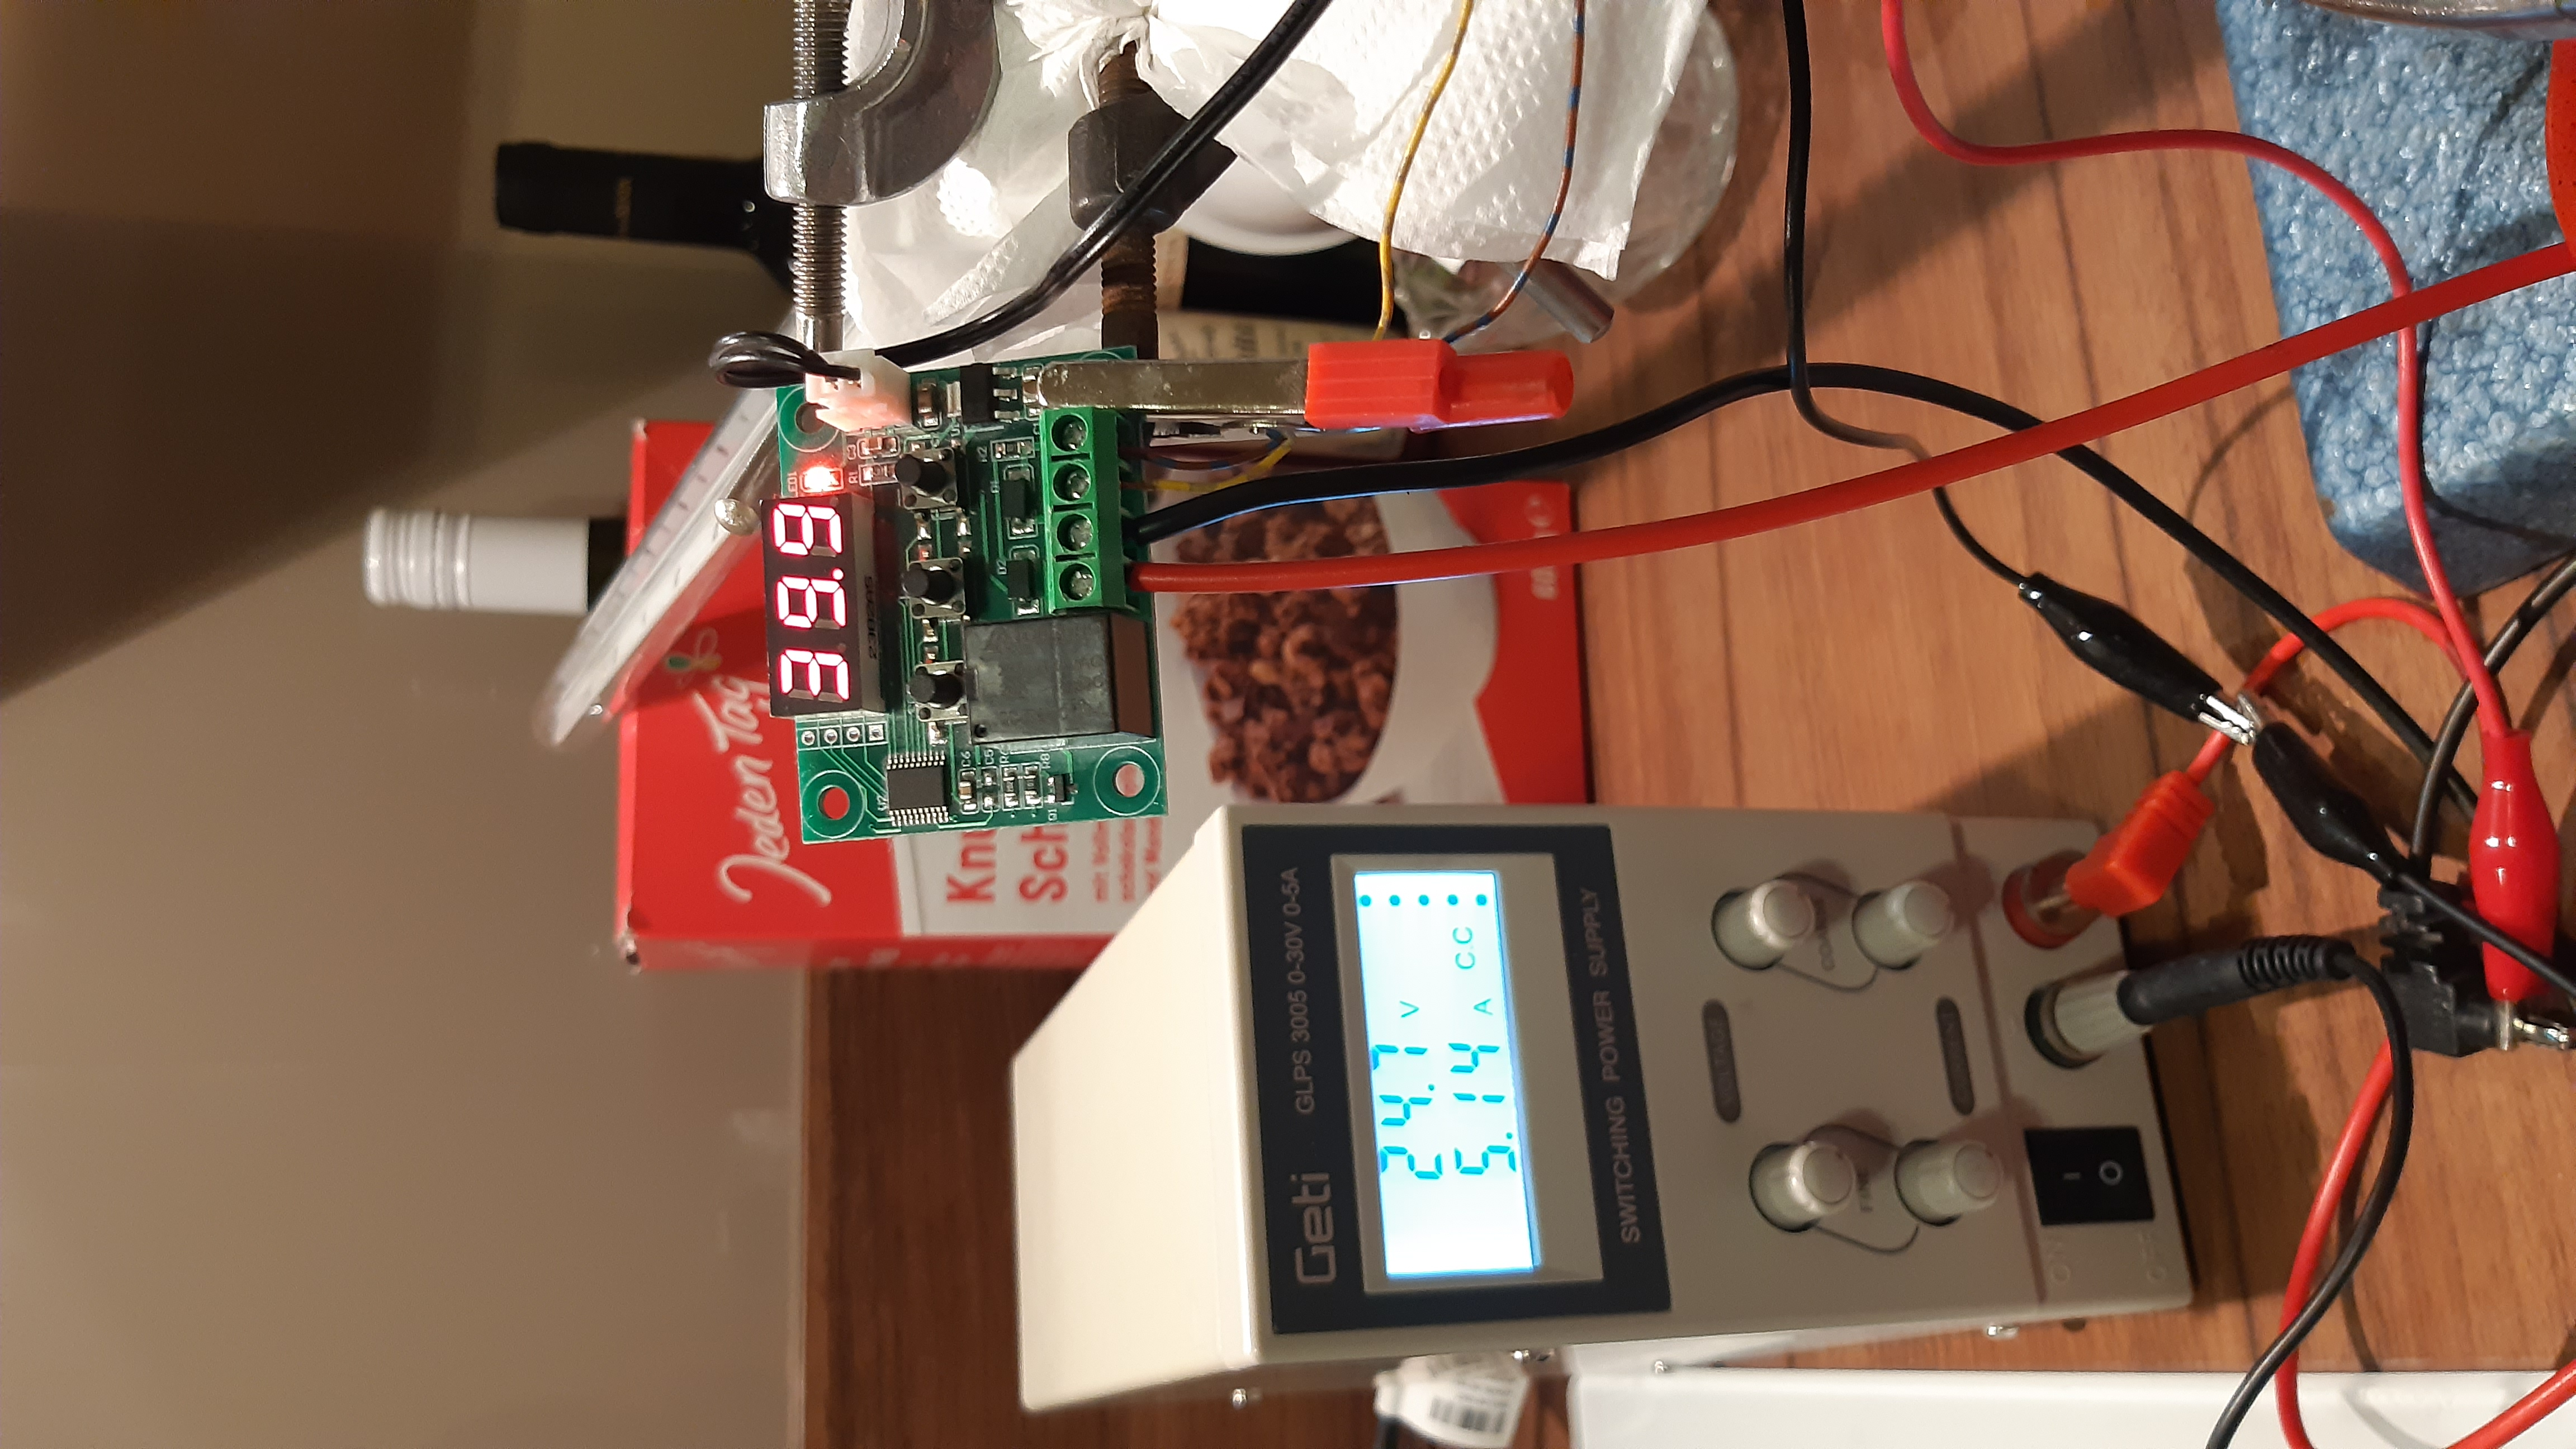
\includegraphics[angle = 270, width = \textwidth]{prilohy/elektro.jpg}
        \caption{Detail termostatu a~laboratorního zdroje stejnosměrného napětí. Termostat indikuje teplotu lázně \SI{39,9}{\degreeCelsius} a~červená LED svítí, ohřev je tedy zapnutý (nastavená teplota byla \SI{40,0}{\degreeCelsius}). Na termostat je v~horní části napojena dvojice černých vodičů, na které je napojeno čidlo (termistor) umístěné v~lázni. Ve spodní části je do svorkovnice termostatu zapojena dvojice tlustých vodičů (červený a~černý), které napájejí topné těleso, a~dvojice tenkých vodičů (hnědo-modrý a~žluto-šedivý), které napájejí samotný termostat. Laboratorní zdroj indikuje napětí \SI{24,7}{\volt} a~proud \SI{5,14}{\ampere}, kterým je topné těleso napájeno.}
    \end{subfigure}
    \caption{Pohled na druhou implementaci aparatury z~vrchu (vlevo) a~detail laboratorního zdroje a~termostatu (vpravo).}
    \label{fig:elektro}
\end{figure}

\begin{figure}[h!]
    \begin{subfigure}[b]{\textwidth}
        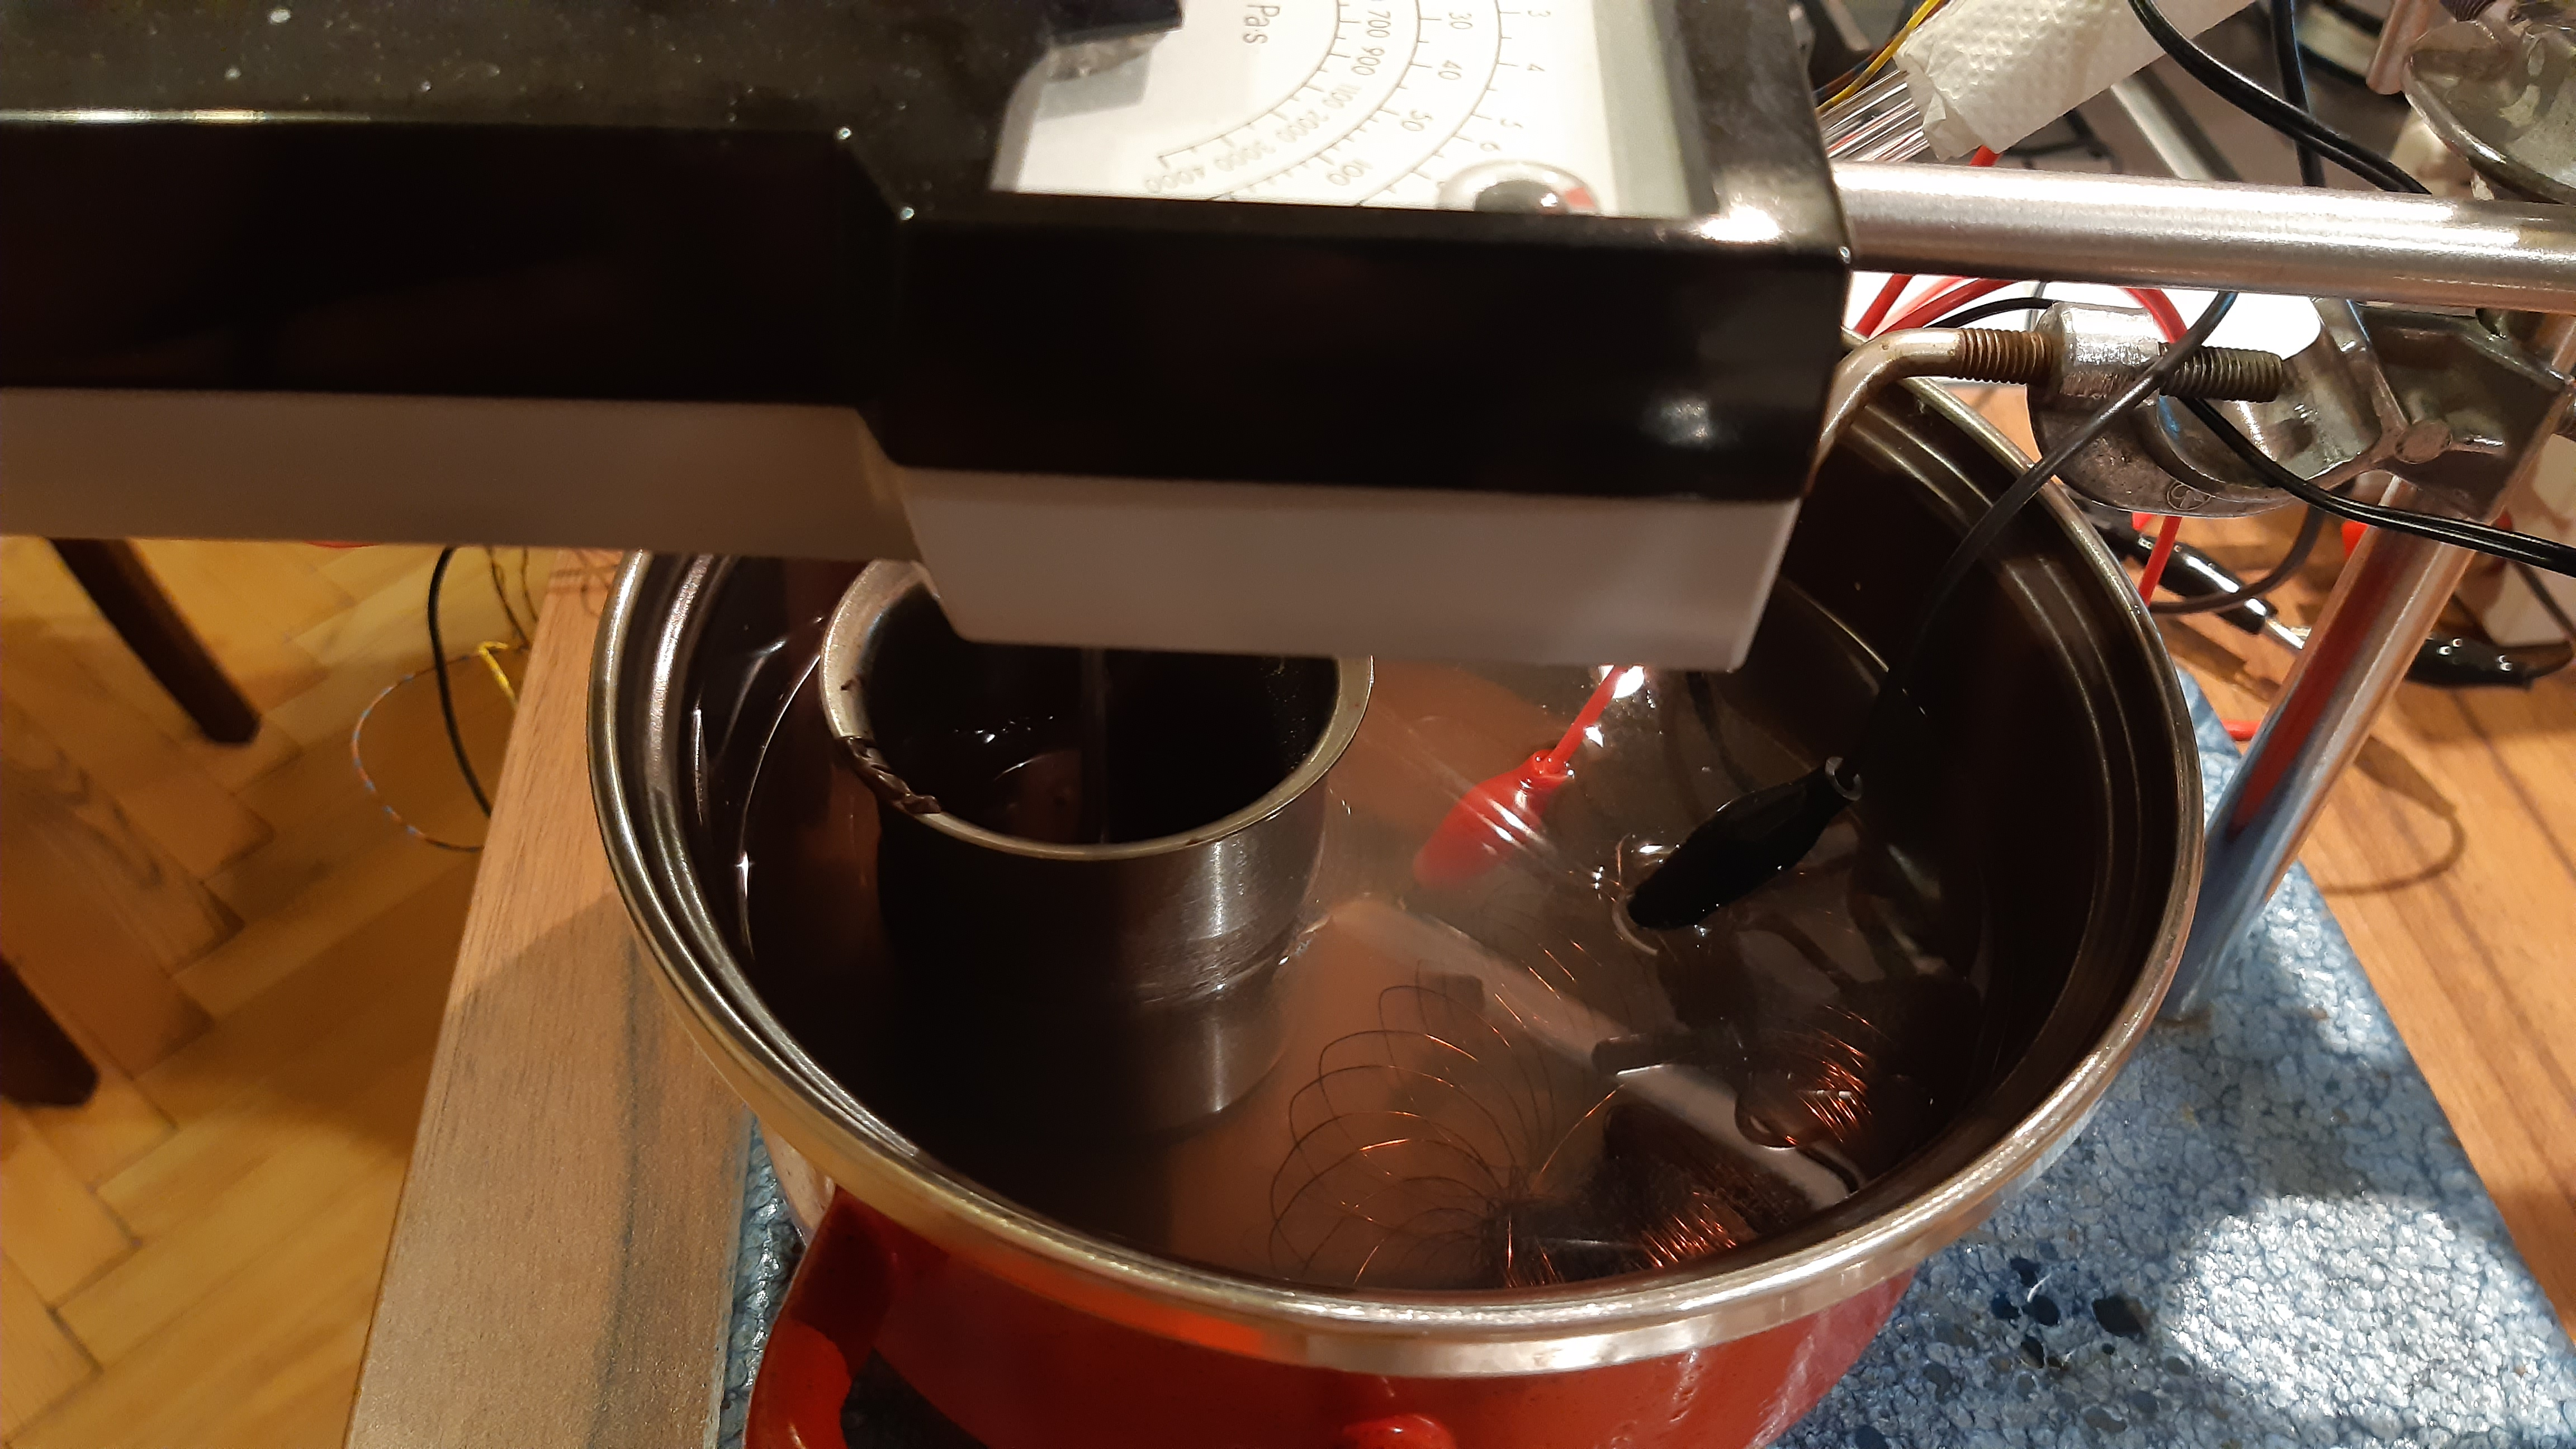
\includegraphics[width = \textwidth]{prilohy/lázeň_1.jpg}
        \caption{Detail lázně. V~kovové kádince se nachází čokoládová tavenina, do které je ponořeno měřicí vřeteno viskozimetru. V~lázni je umístěna cívka smotaná z~měděného drátu, která tvoří topné těleso.}
    \end{subfigure}
    \hfill
    \begin{subfigure}[b]{\textwidth}
        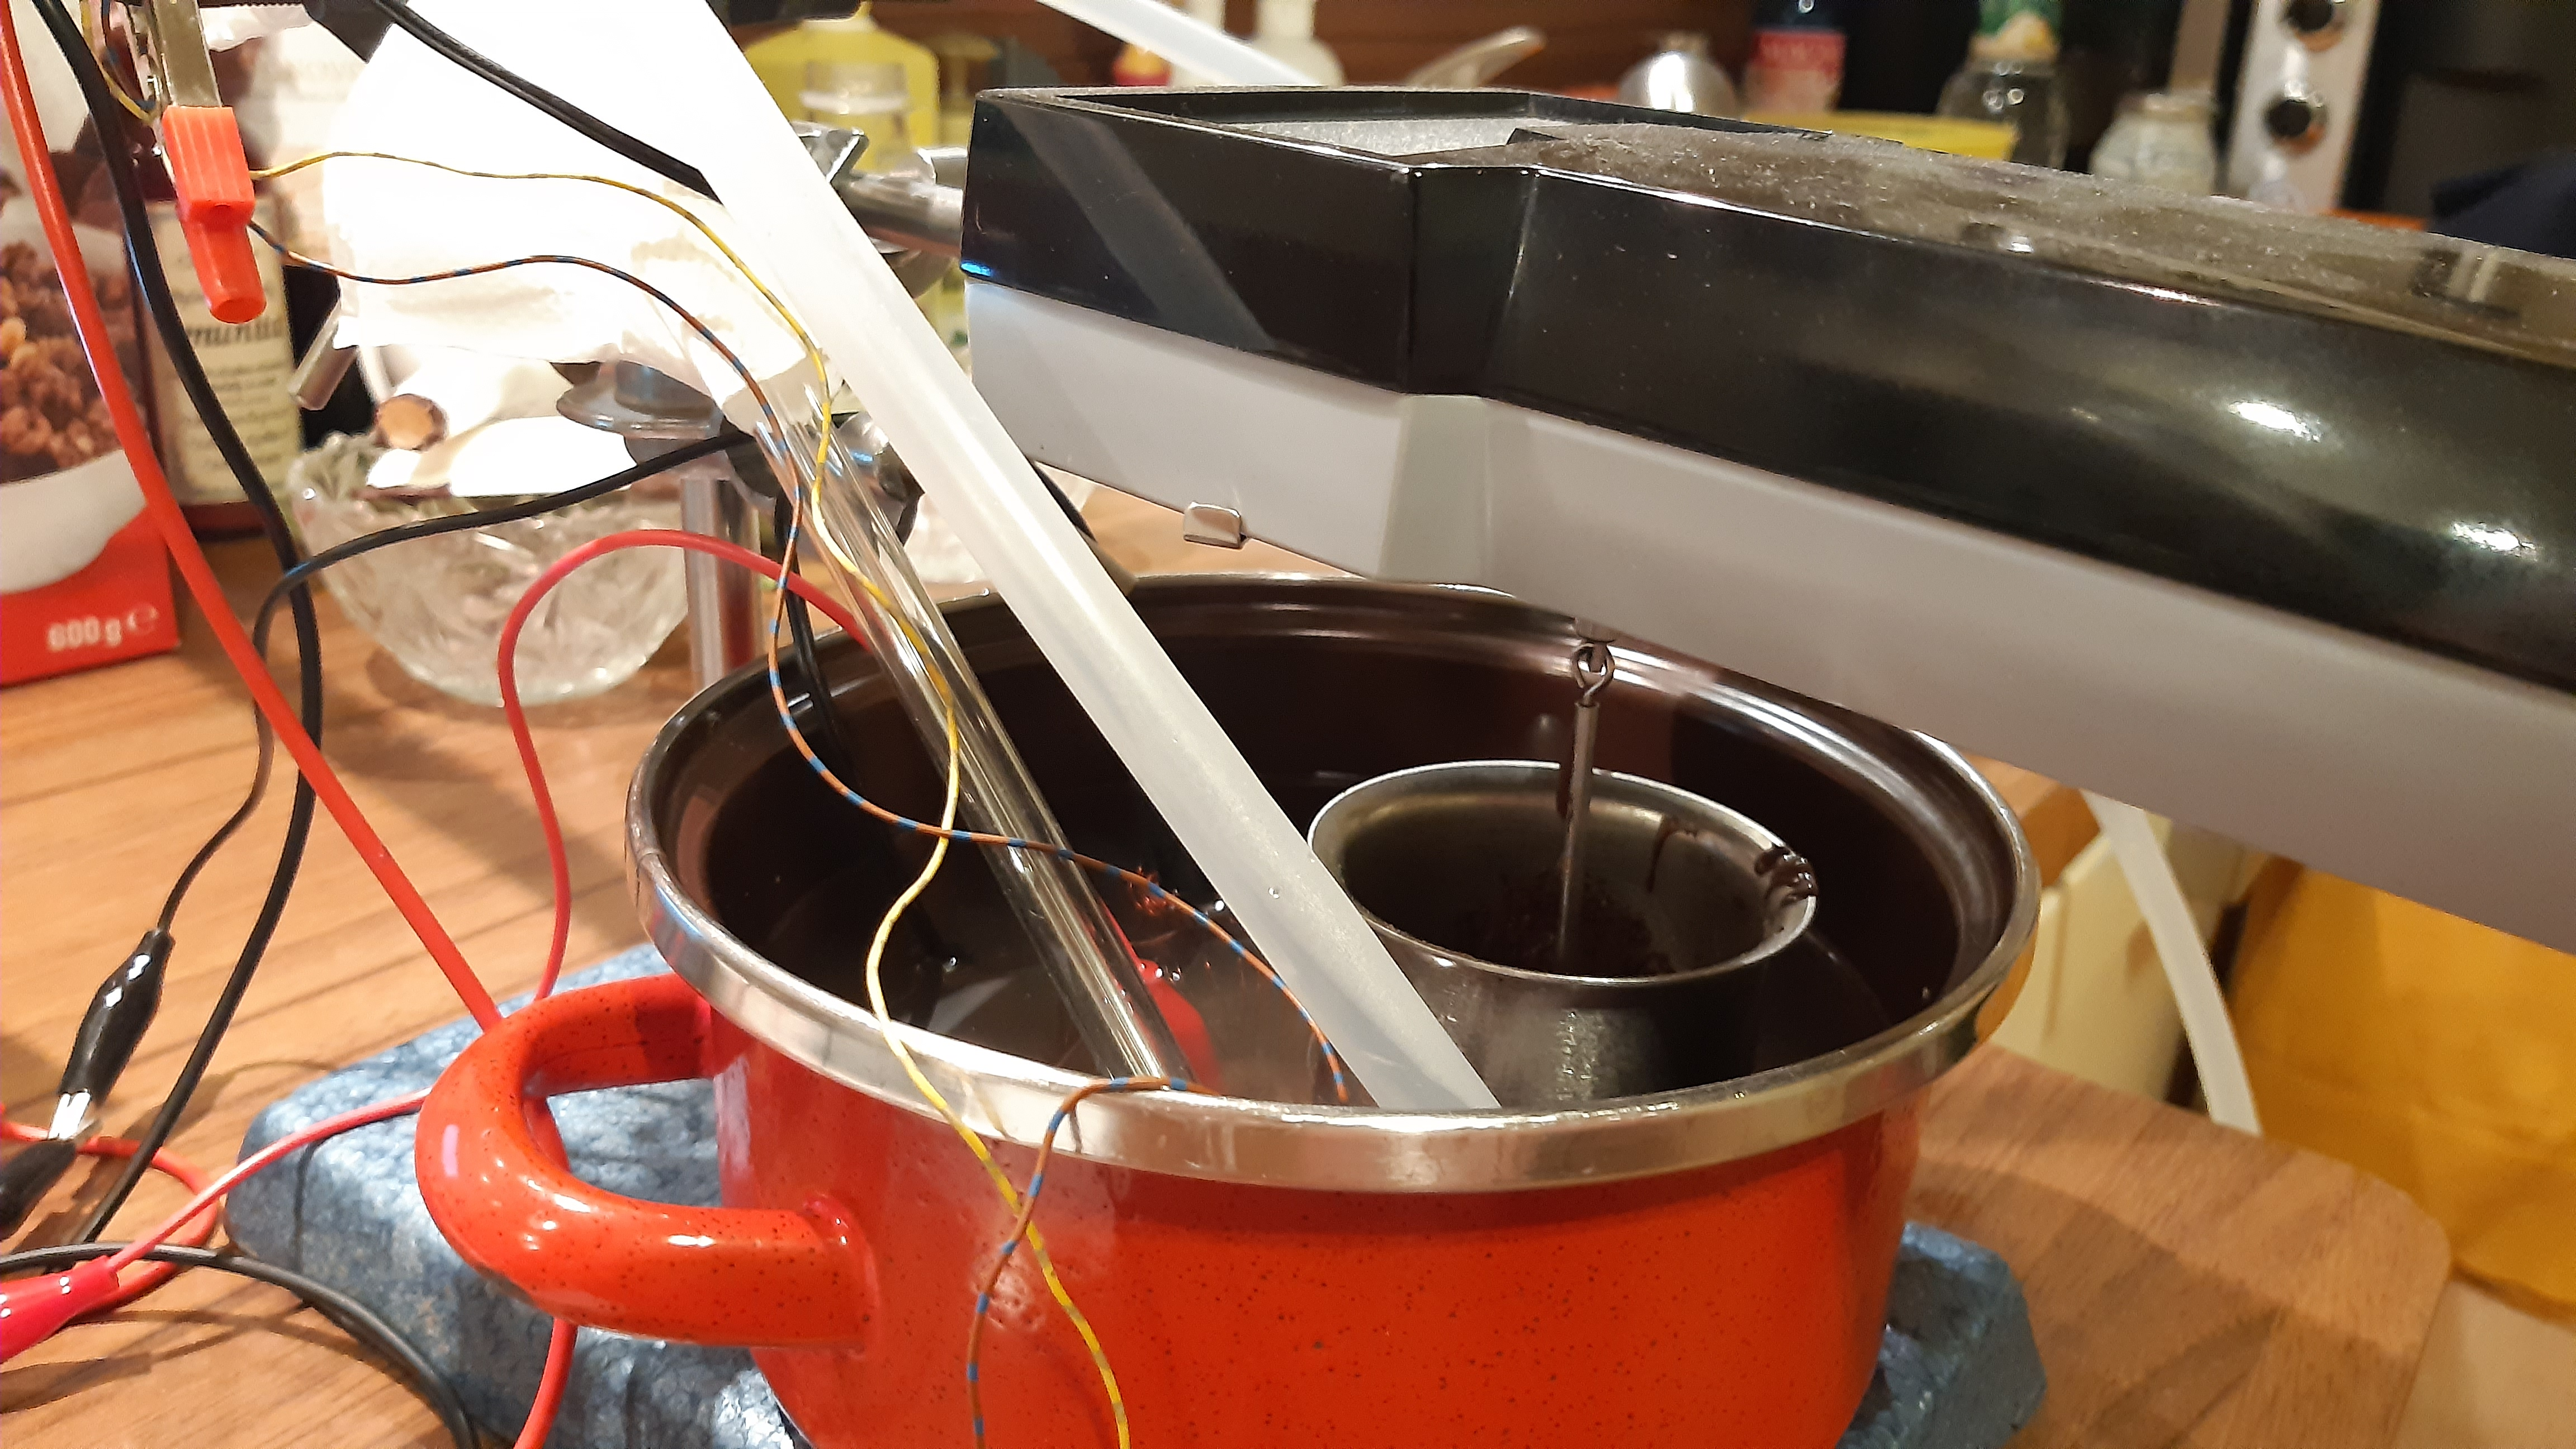
\includegraphics[width = \textwidth]{prilohy/lázeň_2.jpg}
        \caption{Detail lázně. V~kovové kádince se nachází čokoládová tavenina, do které je ponořeno měřicí vřeteno viskozimetru. Z~lázně vede plastová hadička určená k~odčerpávání přebytečné vody z~lázně. Vedle ní je vidět stonek rtuťového teploměru.}
    \end{subfigure}
    \caption{Detail lázně.}
    \label{fig:lazen}
\end{figure}

\begin{figure}[h!]
    \begin{subfigure}[b]{.5\textwidth}
        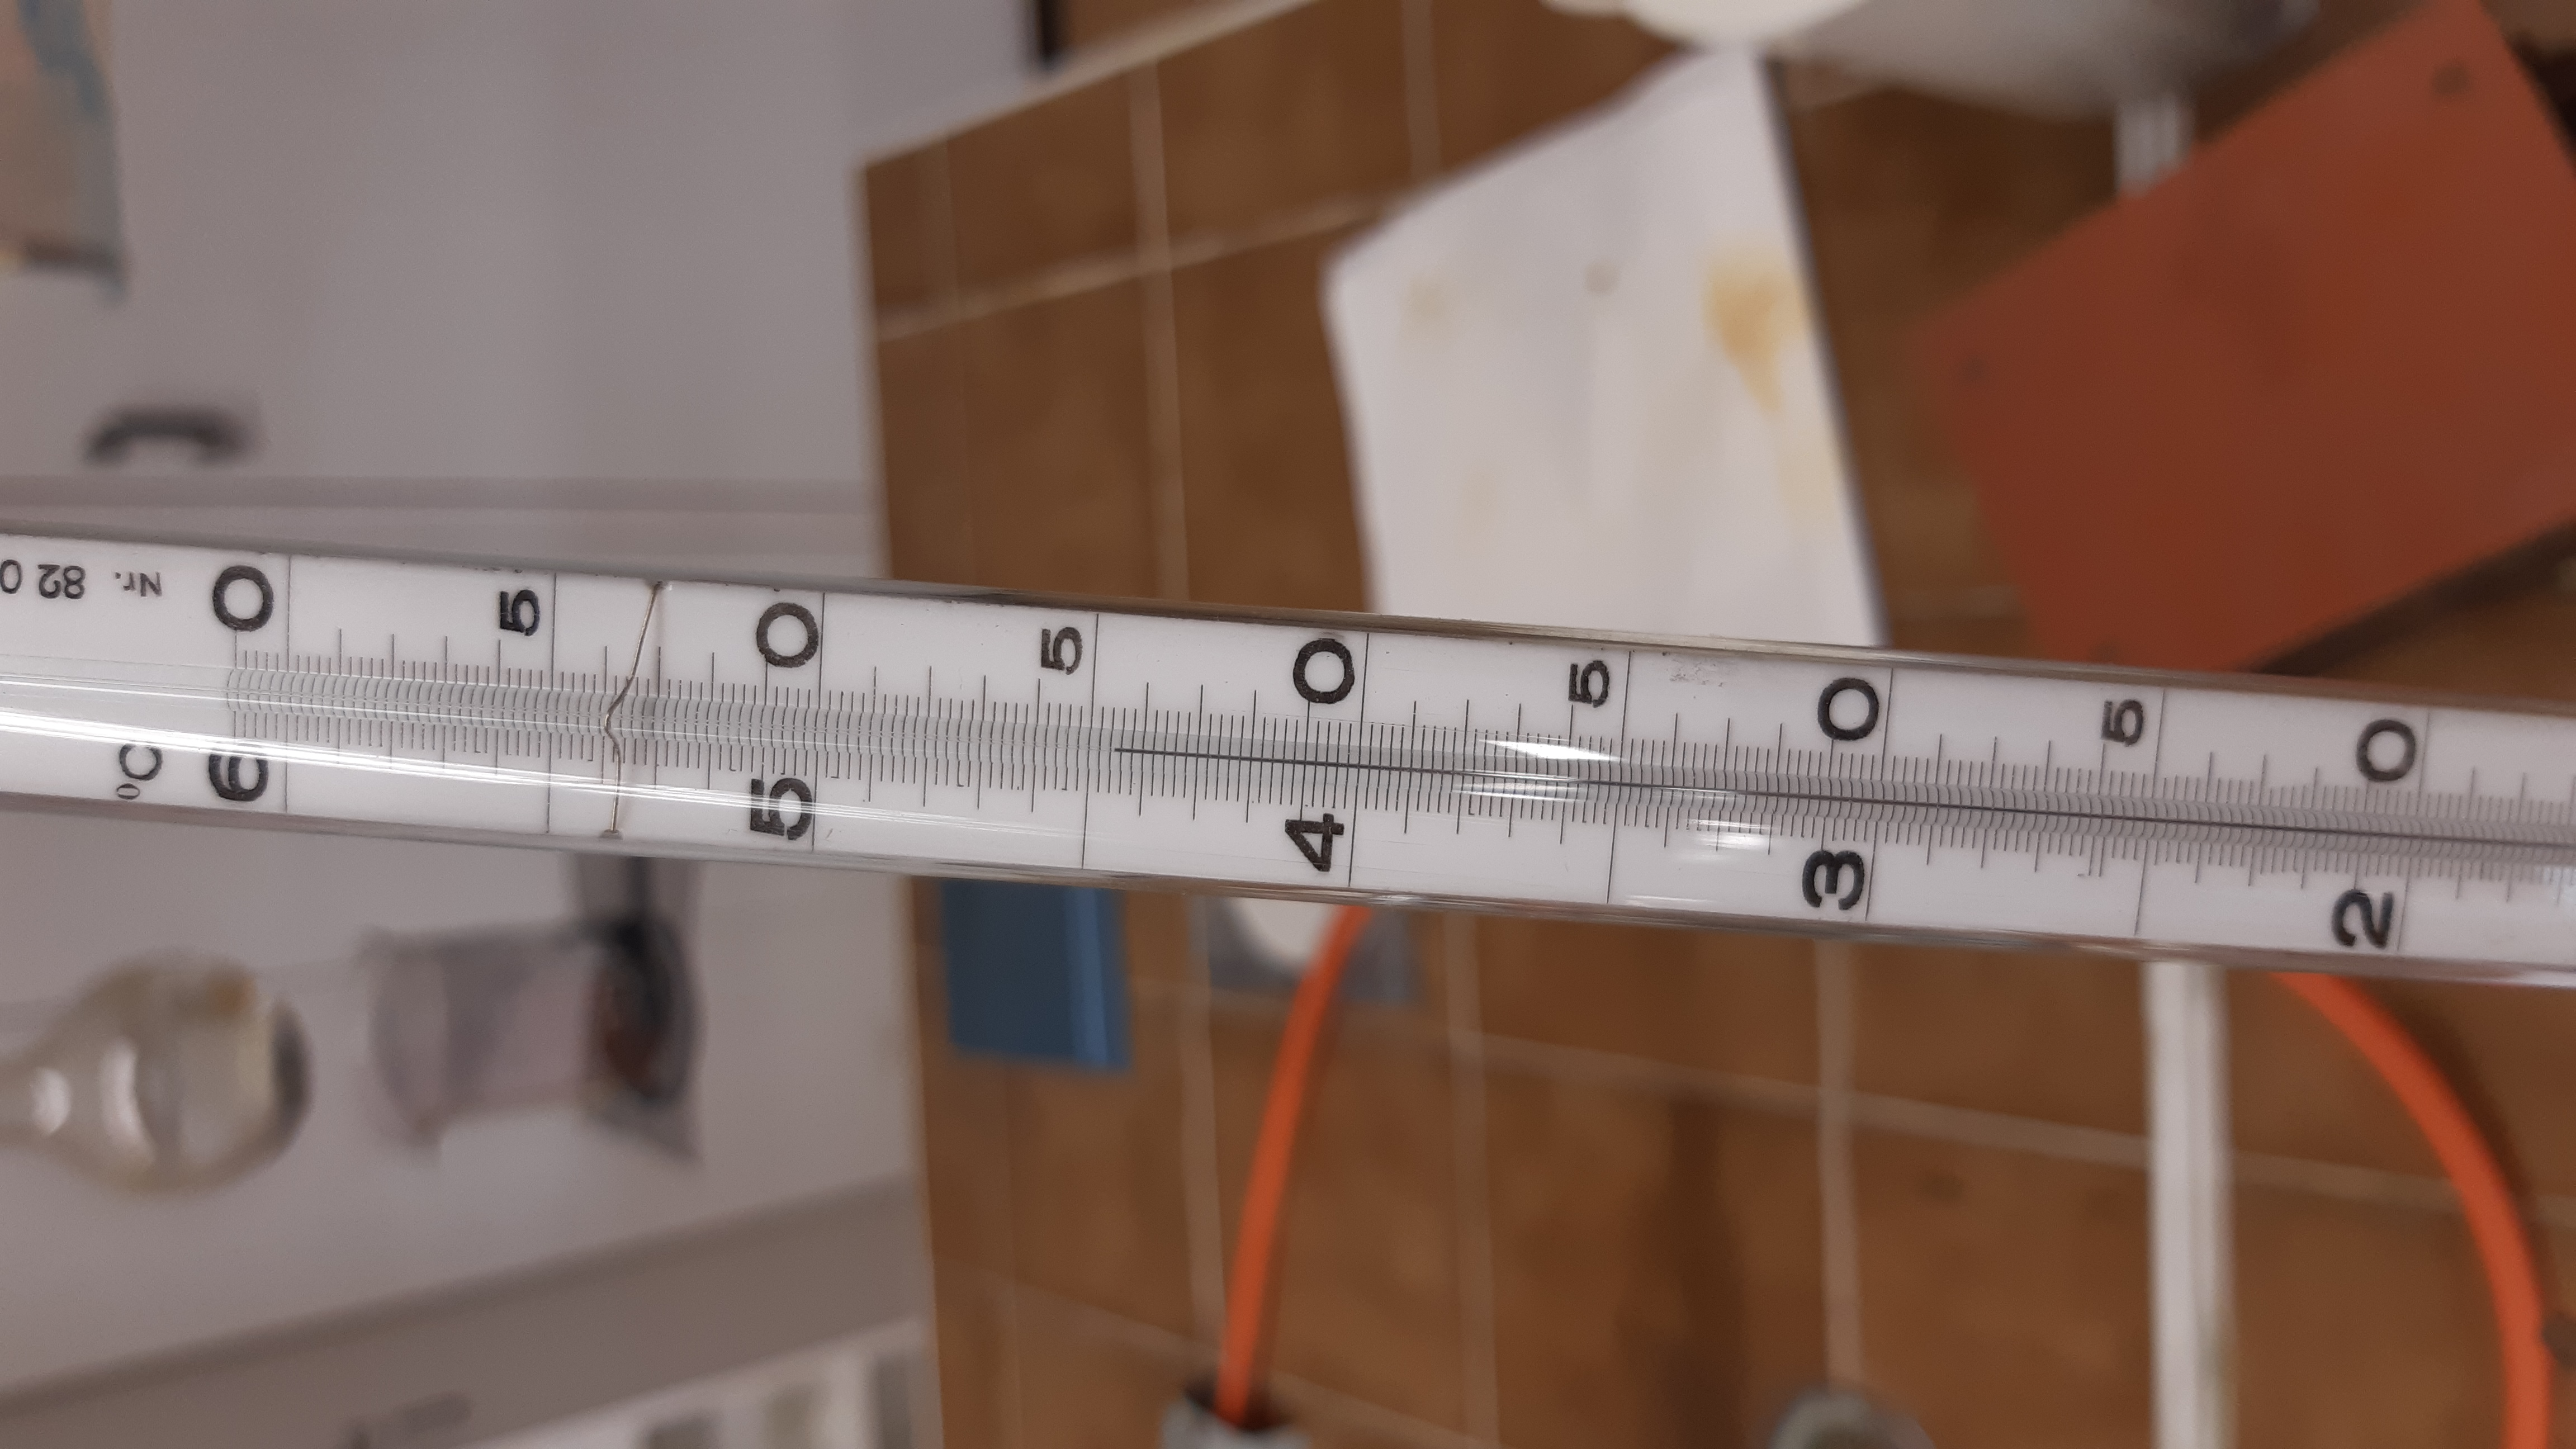
\includegraphics[angle = 270, width = \textwidth]{prilohy/teploměr_1.jpg}
    \end{subfigure}
    \hfill
    \begin{subfigure}[b]{.5\textwidth}
        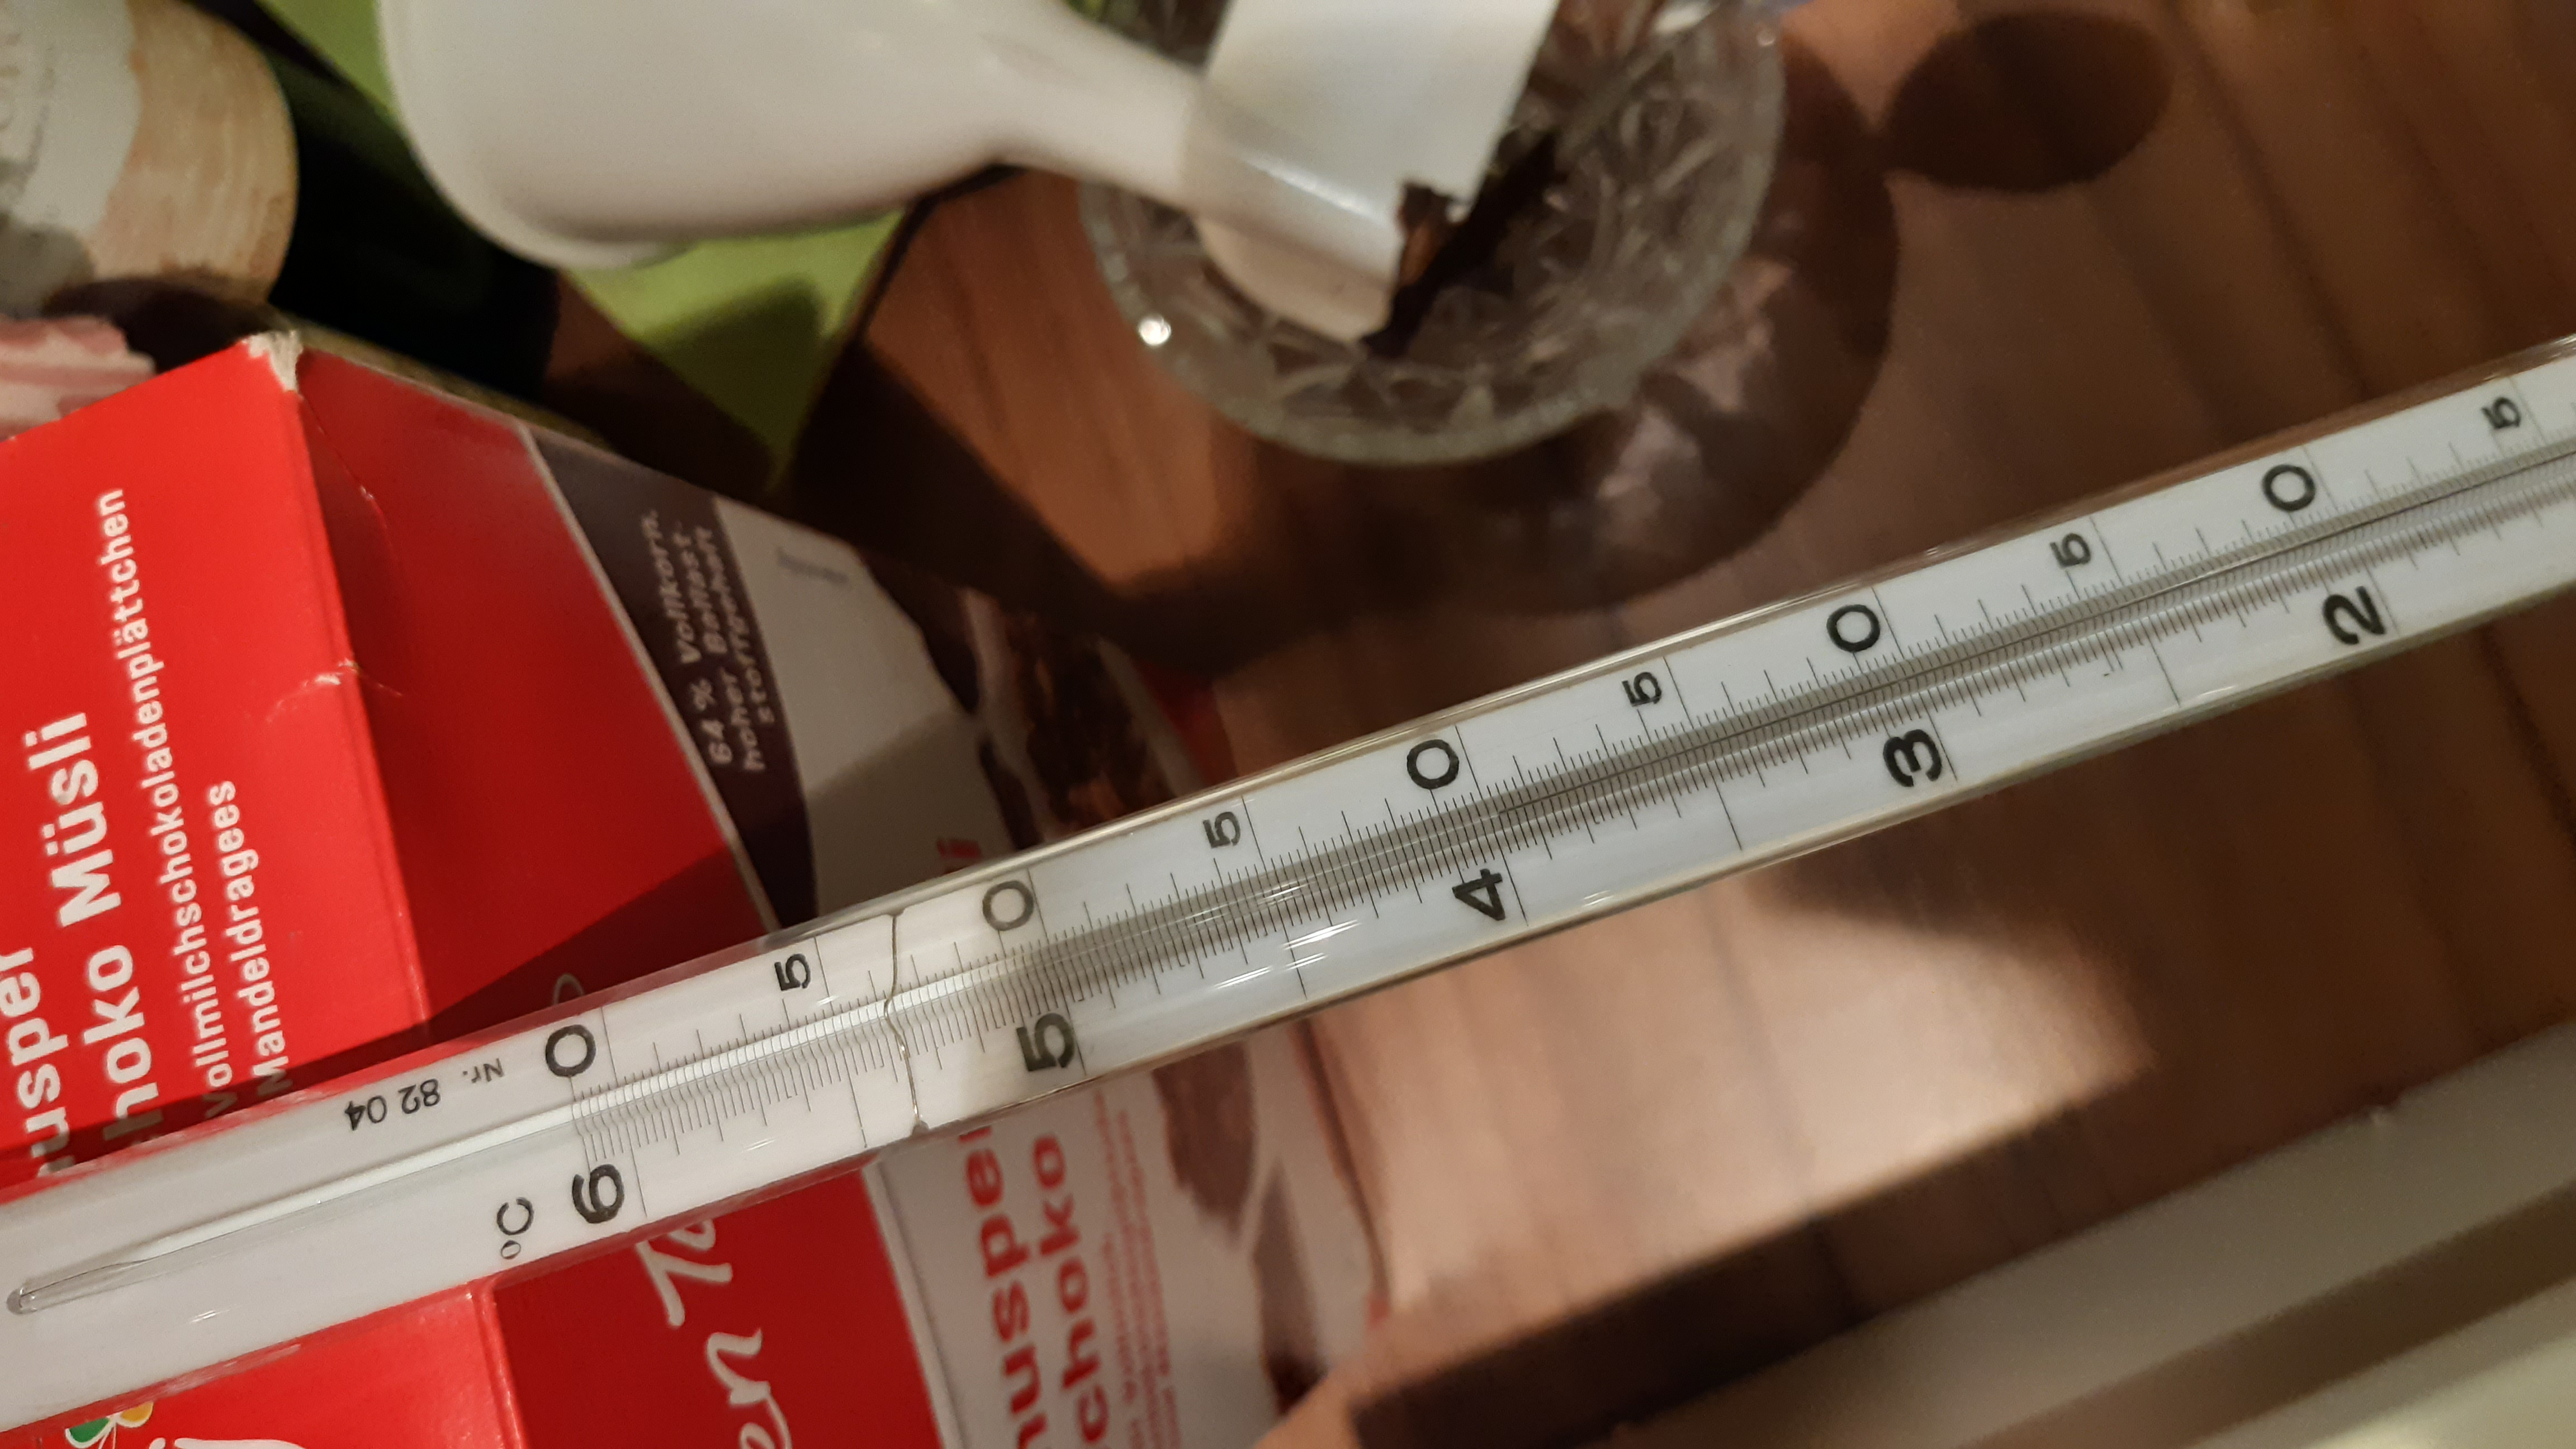
\includegraphics[angle = 270, width = \textwidth]{prilohy/teploměr_2.jpg}
    \end{subfigure}
    \caption{Teploměr použitý k~měření teploty lázně. Jedná se o~meteorologický půdní lomený teploměr (více informací na str.~\pageref{sec:teploměr}). Na levém obrázku je naměřená teplota \SI{44,5}{\degreeCelsius}, na pravém \SI{39,8}{\degreeCelsius}.}
    \label{fig:teploměr}
\end{figure}

\end{document}
